\documentclass[ack,preface]{diphdthesis}

\usepackage[backend=biber,bibencoding=ascii,style=numeric-comp,mincrossrefs=20]{biblatex}
\usepackage{bookmark}
\usepackage{booktabs} % cmidrule, toprule, etc
\usepackage{caption}
\usepackage{epigraph}
\usepackage{graphicx}
\usepackage{hhline} % double lines, instead of \cline
\usepackage{hyperref}
\usepackage[utf8]{inputenc}
\usepackage{minted}
\usepackage{multirow}
\usepackage[defblank]{paralist} % inparaenum
\usepackage[skip=0cm,list=true,labelfont=it]{subcaption}
\usepackage{wrapfig}
\usepackage[dvipsnames]{xcolor}
\usepackage{xparse} % NewDocumentCommand

\usepackage{definitions/code}
\usepackage{definitions/instructions}
\usepackage{definitions/mathpartir} % inference rules
\usepackage{definitions/misc}

\renewcommand{\textflush}{flushepinormal} % justify in epigraph

%%%% TEMPORARY %%%%
%\usepackage{comment}
%\usepackage{pagecolor}
%\pagecolor{black}
%\color{white}
\newcommand{\todo}{\textbf{\textcolor{Red}{FIX???}}}
\newcommand{\dlarrow}{\textcolor{Bittersweet}{CHANGE!!!}}
%%%% TEMPORARY %%%%

%%%% Metadata START %%%%
\authorFirstEn{George}
\authorFirstAbrEn{G.} % abbreviation of first name
\authorMiddleEn{S.}   % abbreviation of father's first name
\authorLastEn{Kastrinis}
\authorFirstGr{Γεώργιος}
\authorFirstAbrGr{Γ.}
\authorMiddleGr{Σ.}
\authorLastGr{Καστρίνης}

%\titleEn{Precision, Completeness and Scalability for Static Pointer Analysis}
\titleEn{Static Pointer Analysis: A Story of Scalable and  High-Confidence Results}
%\titleEn{Scalable Static Pointer Analysis with High-Confidence Results}
\titleGr{Αποδοτική Στατική Ανάλυση Δεικτών με Αξιόπιστα Αποτελέσματα}

% Month followed by Year
\dateGr{ΜΑΙΟΣ 2019}
\dateEn{MAY 2019}

% Advisor info
\advisorGr{Γιάννης Σμαραγδάκης}
\advisorRankGr{Καθηγητής}
\advisorOrgGr{ΕΚΠΑ}
\advisorEn{Yannis Smaragdakis}
\advisorRankEn{Professor}
\advisorOrgEn{NKUA}

% Members of the advisory board 
% (the first one, will be automatically taken up by the advisor)
\boardTwoGr{Αλέξης Δελής}
\boardTwoRankGr{Καθηγητής}
\boardTwoOrgGr{ΕΚΠΑ}
\boardTwoEn{Alex Delis}
\boardTwoRankEn{Professor}
\boardTwoOrgEn{NKUA}

\boardThreeGr{Παναγιώτης Ροντογιάννης}
\boardThreeRankGr{Καθηγητής}
\boardThreeOrgGr{ΕΚΠΑ}
\boardThreeEn{Panos Rondogiannis}
\boardThreeRankEn{Professor}
\boardThreeOrgEn{NKUA}

% 7 Member examination committee
% (the first three will be taken up by the advisory board)
%%%%%%%%%%% TEMPORARY %%%%%%%%%%%
\examFourGr{Μέμα Ρουσσοπούλου}
\examFourRankGr{Αναπληρώτρια Καθηγήτρια}
\examFourOrgGr{ΕΚΠΑ}
\examFourEn{Mema Roussopoulos}
\examFourRankEn{Associate Professor}
\examFourOrgEn{NKUA}

\examFiveGr{Μανόλης Κουμπαράκης}
\examFiveRankGr{Καθηγητής}
\examFiveOrgGr{ΕΚΠΑ}
\examFiveEn{Manolis Koubarakis}
\examFiveRankEn{Professor}
\examFiveOrgEn{NKUA}

\examSixGr{Νικόλαος Παπασπύρου}
\examSixRankGr{Αναπληρωτής Καθηγητής}
\examSixOrgGr{ΕΜΠ}
\examSixEn{Nikolaos Papaspyrou}
\examSixRankEn{Associate Professor}
\examSixOrgEn{NTUA}

\examSevenGr{???}
\examSevenRankGr{Αναπληρωτής Καθηγητής}
\examSevenOrgGr{???}
\examSevenEn{???}
\examSevenRankEn{Associate Professor}
\examSevenOrgEn{???}

% The examination date of the thesis
\examinationDateGr{1 Μαΐου 2019}
\examinationDateEn{May 1, 2019}


%%%% Abstract, synopsis, inscription, acknowledgments, and preface pages %%%%
\abstractEn{Static program analysis aims to automatically reason about certain properties a given program might exhibit under all possible executions without actually observing such executions. Static \emph{pointer} analysis is a major subcategory that focuses on the objects that program expressions might point during program executions. The evolution of programming languages has lead to the addition of many abstraction layers, that as a result have made any automatic reasoning about a program a challenging task at best or an infeasible one at worst. Thus, any practical static pointer analysis algorithm has to compromise and aim to approximate results in some way---either computing more or less that what is actually true.

This dissertation shows how we can obtain \emph{precise} yet also \emph{scalable} static pointer analysis algorithms by carefully differentiating policies for different parts of the program. Furthermore, since a static pointer analysis algorithm with global soundness guarantees and meaningful results throughout is not realistic, we show that it is possible to design analyses that offer \emph{strong guarantees} on the soundness of the results for specific parts of the program.

Pointer analyses in the past introduced the concept of \emph{context-sensitivity} in order to tackle the ever growing problem of imprecision versus scalability. Context is used to annotate analysis components so that the analysis can be more precise without at the same time sacrificing scalability. We show beneficial ways to combine different context flavors for different parts of the program without paying the cost that a naive combination would incur.

Another attempt at producing precise yet scalable analyses leads us to an introspective analysis. We employ a common adaptive pattern in which a cheap imprecise analysis is run first so various metrics can be gathered, and then a more precise (and costly) analysis can be used only in parts of the program---under the assumption that more precise handling of the rest would only incur performance penalties.

Subsequently, we shift our attention to an analysis that \emph{under}-approximates results (instead of the norm of \emph{over}-approximating) so that it might report less but can guarantee those properties to always hold. We build upon observations on the properties that such analyses have in order to apply a specialized data structure that speeds up our algorithm by nearly two orders of magnitude.

Finally, in our last contribution, we revisit an analysis formulation that overapproximates results to create an analysis algorithm that is truly sound but at the same time highly efficient. Our analysis is conservative, guaranteeing soundness even in the presence of arbitrary unknown code, but avoids wasting any work on computations that will later be invalidated due to soundness concerns.}
\abstractGr{Η στατική ανάλυση στοχεύει στον αυτόματο συμπερασμό ιδιοτήτων που κάποιο πρόγραμμα μπορεί να επιδείξει σε κάθε πιθανή εκτέλεση, χωρίς στην πράξη να εκτελείται. Η στατική ανάλυση \emph{δεικτών} αποτελεί μια μεγάλη υποκατηγορία της που επικεντρώνεται στα δυναμικά αντικείμενα που δύνανται να ``δείξουν'' οι εκφράσεις ενός προγράμματος σε κάποια εκτέλεση του. Η εξέλιξη των γλωσσών προγραμματισμού με την πάροδο των χρόνων οδήγησε στην προσθήκη πολλών επιπέδων αφαίρεσης, τα οποία σαν αποτέλεσμα έχουν ο αυτόματος συμπερασμός για κάποιο πρόγραμμα να αποτελεί τουλάχιστον μία πρόκληση αν όχι και μία αδύνατη προσπάθεια. Συνεπώς, κάθε πρακτικός αλγόριθμος στατικής ανάλυσης πρέπει να στοχεύσει σε μια εκτίμηση των πραγματικών αποτελεσμάτων με κάποια μορφή ανακρίβειας---είτε υπολογίζοντας περισσότερα είτε λιγότερα.

Σε αυτή τη διατριβή παρουσιάζουμε πώς μπορούμε να σχεδιάσουμε \emph{ακριβείς} και συνάμα \emph{αποδοτικούς} αλγορίθμους ανάλυσης δεικτών εφαρμόζοντας διαφορετικές πολιτικές σε διαφορετικά σημεία του προγράμματος. Συμπληρωματικά, δεδομένου ότι ένας αλγόριθμος ανάλυσης δεικτών με βεβαιώσεις εγκυρότητας για όλα τα σημεία του προγράμματος καθώς και πρακτικά αποτελέσματα δεν αποτελεί ρεαλιστική κατεύθυνση, δείχνουμε πώς μπορούμε να σχεδιάσουμε αναλύσεις με \emph{ισχυρές βεβαιώσεις εγκυρότητας} για συγκεκριμένα κομμάτια ενός προγράμματος.

Προηγούμενοι αλγόριθμοι για ανάλυση δεικτών εισήγαγαν την έννοια των \emph{συμφραζομένων} ({\en context}) για να αντιμετωπίσουν το αυξανόμενο πρόβλημα της ανακρίβειας έναντι της αποδοτικότητας. Τα συμφραζόμενα χρησιμοποιούνται για να επαυξήσουν στοιχεία της ανάλυσης ώστε η ανάλυση να καταφέρει να είναι πιο ακριβής χωρίς ταυτόχρονα να πρέπει να κάνει θυσίες στον τομέα της αποδοτικότητας. Παρουσιάζουμε επωφελείς τρόπους συνδυασμού διάφορων ειδών συμφραζομένων σε διαφορετικά σημεία του προγράμματος, χωρίς αυτοί οι συνδυασμοί να επιφέρουν το κόστος που θα παρουσίαζε μία αφελής προσέγγιση.

Μία δεύτερη απόπειρα για δημιουργία αναλύσεων που παρουσιάζουν υψηλή ακρίβεια και αποδοτικότητα μας οδηγεί σε μια ανάλυση \emph{ενδοσκόπησης} ({\en introspection}). Εφαρμόζουμε ένα σύνηθες μοτίβο στο οποίο μια φτηνή ανακριβής ανάλυση εφαρμόζεται πρώτη ώστε να συλλέξει διάφορες μετρικές για το πρόγραμμα, και στη συνέχεια μια δεύτερη πιο ακριβής (και ακριβή) ανάλυση μπορεί να εφαρμοστεί μόνο σε συγκεκριμένα σημεία του προγράμματος---υπό την υπόθεση ότι η πιο ακριβής μεταχείριση των υπολοίπων θα είχε μόνο αρνητικά αποτελέσματα στην συνολική απόδοση.

Εν συνεχεία, μετατοπίζουμε την προσοχή μας προς μια ανάλυση που \emph{υπό}-εκτιμά τα αποτελέσματα της (σε αντίθεση με το σύνηθες των αναλύσεων που υπολογίζουν μία \emph{υπέρ}-εκτίμηση). Με αυτή την αντιμετώπιση, η ανάλυση μας αναφέρει λιγότερα αποτελέσματα αλλά μπορεί να παρέχει ισχυρές βεβαιώσεις ότι αυτά θα ισχύουν πάντα. Βασιζόμενοι πάνω σε παρατηρήσεις για τις ιδιότητες που παρουσιάζουν αναλύσεις αυτού του είδους, εφαρμόζουμε μια ειδική δομή δεδομένων η οποία επιφέρει επιταχύνσεις στον αλγόριθμο μας σχεδόν κατά δύο τάξεις μεγέθους.

Τέλος, στην τέταρτη συνεισφορά της διατριβής, επιστρέφουμε ξανά στην οικογένεια αναλύσεων που υπερεκτιμούν τα αποτελέσματα τους. Ο στόχος μας είναι η δημιουργία ενός αρκετά αποδοτικού αλγορίθμου που όντως παράγει έγκυρα αποτελέσματα χωρίς περιορισμούς στο υποκείμενο πρόγραμμα. Κατά συνέπεια, αυτό μας οδηγεί σε μία συντηρητική ανάλυση, που μπορεί να παρέχει βεβαιώσεις εγκυρότητας ακόμα και υπό την παρουσία άγνωστου κώδικα, αλλά ταυτόχρονα αποφεύγει την σπατάλη υπολογισμών σε δεδομένα που αργότερα θα χρειαστεί να ανατραπούν για την διατήρηση των βεβαιώσεων αυτών.}
\synopsisGr{Η διατριβή αυτή ανήκει στον ευρύτερο τομέα της στατικής ανάλυσης προγραμμάτων, η οποία στοχεύει στον αυτόματο συμπερασμό για τις ιδιότητες που παρουσιάζει κάποιο πρόγραμμα με βάση την εξέταση του πηγαίου του κώδικα (ή κάποιας αντίστοιχης ενδιάμεσης αναπαράστασης), αλλά δίχως να απαιτείται πραγματική εκτέλεση του. Η δουλειά μας στην διατριβή αυτή επικεντρώνεται σε μια μεγάλη υποκατηγορία της στατικής ανάλυσης, αυτή της ανάλυσης \emph{δεικτών}. Μία ανάλυση δεικτών στοχεύει στο να υπολογίσει τα σύνολα αντικείμένων στα οποία μπορεί να ``δείξει'' κάθε έκφραση του προγράμματος (π.χ. τοπική μεταβλητή, ή κάποιο πεδίο, κτλ.) σε όλες τις πιθανές εκτελέσεις του.

Σαν αποτέλεσμα, κάθε πρακτικός αλγόριθμος που στοχεύει να παρέχει ουσιαστικά αποτελέσματα αναγκάζεται να κάνει έναν πρώτο συμβιβασμό: χρειάζεται να κατασκευαστεί κάποιο \emph{αφηρημένο} μοντέλο της μνήμης, όπου \emph{εικονικά} αντικείμενα αναπαριστούν (μία ή περισσότερες) \emph{διακριτές} δεσμεύσεις πραγματικών αντικειμένων. Ένα κλασικό παράδειγμα αυτού είναι η δέσμευση αντικειμένων από κάποια εντολή μέσα σε κάποια δομή επανάληψης. Η συνηθισμένη αντιμετώπιση από κάποιον αλγόριθμο ανάλυσης δεικτών είναι να θεωρηθούν όλα τα αντικείμενα που εν δυνάμει θα δεσμευτούν από την ίδια εντολή σαν ένα μοναδικό, αφηρημένο αντικείμενο. Αυτό αποτελεί μία (από τις πολλές) πήγη ανακρίβειας στα αποτελέσματα της όποιας ανάλυσης. Ταυτόχρονα όμως, συμβιβασμοί σαν αυτόν, αν και οδηγούν σε εκτιμήσεις της συμπεριφοράς ενός προγράμματος και όχι σε απόλυτα αποτελέσματα, επιτρέπουν στις αναλύσεις να κάνουν πολύπλοκους αυτόματους συμπερασμούς. Συμπερασμοί που βοηθούν σε πληθώρα τομέων όπως η μηχανικά υποβοηθούμενη κατανόηση του προγράμματος, η εύρεση σφαλμάτων, και η βελτιστοποίηση της απόδοσης του προγράμματος.

Τα παραπάνω φανερώνουν ένα από τα βαθύτερα προβλήματα κάθε αλγορίθμου στατικής ανάλυσης δεικτών. Δηλαδή ότι, συχνά, ο σχεδιασμός ενός τέτοιου αλγορίθμου είναι αποτέλεσμα ισορροπίας μεταξύ θεμάτων ακριβείας και κλιμάκωσης. Είναι σχετικά απλό μία ανάλυση να επικεντρωθεί στον υπολογισμό αποτελεσμάτων υψηλής ακρίβειας, θυσιάζοντας την γενική απόδοση του αλγορίθμου. Αντίστοιχα, είναι δυνατόν να σχεδιαστούν πολύ αποδοτικοί αλγόριθμοι, οι οποίοι όμως θα υπολογίζουν μεγάλες εκτιμήσεις των (πραγματικών) αποτελεσμάτων οδηγώντας σε μεγάλη ανακρίβεια.

Η διατριβή αυτή στοχεύει στην αντιμετώπιση του παραπάνω προβλήματος, με την κύρια θέση της να συνοψίζεται ώς εξής:

\begin{displayquote}
Είναι δυνατόν να σχεδιαστούν αλγόριθμοι στατικής ανάλυσης δεικτών που παρουσιάζουν \emph{υψηλή ακρίβεια} αλλά και \emph{κλιμάκωση}, εφαρμόζοντας προσεκτικά διαφορετικές πολιτικές σε διαφορετικά σημεία του προγράμματος. Συμπληρωματικά, είναι δυνατόν να σχεδιαστούν αναλύσεις που προσφέρουν \emph{ισχυρές εγγυήσεις ορθότητας} των αποτελεσμάτων, αλλά για στοχευμένα κομμάτια του προγράμματος.
\end{displayquote}

Στη συνέχεια, θα παρουσιάσουμε διάφορες τεχνικές για την υλοποίηση αποδοτικών αλγορίθμων ανάλυσης δεικτών, στο περιβάλλον της γλώσσας προγραμματισμού {\en Java}, προσαρμόζοντας προσεκτικά την στρατηγική του κάθε αλγορίθμου σε διαφορετικά σημεία του προγράμματος. Επιπροσθέτως, θα παρουσιάσουμε δύο αλγορίθμους αμυντικής φύσης που στοχεύουν στον υπολογισμό αποτελεσμάτων υψηλής εμπιστοσύνης, ακόμη και εν μέσω ``εχθρικού΄΄ ή άγνωστου κώδικα.


\section*{Βασικές Έννοιες της Στατικής Ανάλυσης Δεικτών}

Πριν κάνουμε μια συνοπτική αναφορά των επιστημονικών συνεισφορών της διάτριβης αυτής, είναι απαραίτητο να γίνει μια μικρή εισαγωγή σε βασικές έννοιες της στατικής ανάλυσης (δεικτών), που αποτελούν το επιστημονικό και τεχνικό υπόβαθρο της δουλειάς μας.

\paragraph*{Πλατφόρμα Υλοποίησης \& Γλώσσα υπό Ανάλυση.}
Το μεγαλύτερο μέρος της δουλειάς που θα παρουσιάσουμε στη συνέχεια, είναι υλοποιημένο στην πλατφόρμα {\en \doop{}}\cite{oopsla:2009:Bravenboer}. Το {\en \doop{}} αποτελεί εδώ και χρόνια μία καλά εδραιωμένη πλατφόρμα ανάπτυξης αλγορίθμων στατικής ανάλυσης δεικτών, προσφέροντας μία πληθώρα αναλύσεων που στοχεύουν προγράμματα {\en Java}. Περισσότερες λεπτομέρειες δίνονται στο Κεφάλαιο~\ref{sec:back:doop}.

Αξίζει να σημειωθεί ότι, αν και οι ιδέες και οι αλγόριθμοι που εξερευνούνται παρακάτω επικεντρώνονται γύρω από την ανάλυση προγραμμάτων {\en Java}, δεν είναι παράλογη μία πιθανή γενίκευση τους, σε μικρότερο ή μεγαλύτερο βαθμό, και σε άλλες γλώσσες προγραμματισμού που προσφέρουν παρόμοια χαρακτηριστικά και ακολουθούν παρόμοια μοντέλα/παραδείγματα.


\paragraph*{Χρήση Συμφραζομένων.}
Όπως προαναφέρθηκε, η υλοποίηση κάθε πολύπλοκου αλγορίθμου ανάλυσης δεικτών σύντομα καταλήγει σε μία προσπάθεια εξισορρόπησης μεταξύ ακρίβειας και απόδοσης. Στο παρελθόν, η επιστημονική κοινότητα έχει επεκτείνει το οπλοστάσιο της με διάφορες έννοιες και τεχνικές προς διαχείρηση αυτής της κατάστασης. Μία τέτοια τεχνική, που στοχεύει στην καταπολέμηση της ανακρίβειας των αποτελεσμάτων, ελπίζοντας χωρίς ταυτόχρονα επιβάρυνση της απόδοσης, είναι αυτή των \emph{συμφραζομένων} ({\en context}). Η χρήση των συμφραζομένων (επιπλέον πληροφορίας) γίνεται επαυξάνοντας στοιχεία της εκάστοτε ανάλυσης (π.χ., τοπικές μεταβλητές, πεδία και μεθόδους) ώστε η ανάλυση να καταφέρει να τα χειριστεί με μεγαλύτερη ακρίβεια.

Η κεντρική ιδέα είναι ότι η ανάλυση θα διαφοροποιήσει τον χειρισμό στοιχείων του προγράμματος όταν αυτά συνδυάζονται με κάποια συμφραζόμενα, ενώ θα τα χειριστεί ομοιογενώς όταν συνδυάζονται με κάποια άλλα. Για παράδειγμα, μία ανάλυση μπορεί να εξετάσει διαφορετικά κάποια μεθόδου όταν η κλήση της έγινε μέσα στη μέθοδο \code{A}, μέσα στη μέθοδο \code{B} ή οπουδήποτε αλλού (δηλαδή παρουσιάζοντας τρεις διαφορετικές τιμές συμφραζομένων).

Δύο βασικές κατηγορίες συμφραζομένων έχουν χρησιμοποιηθεί ευρέως στο παρελθόν: τα συμφραζόμενα \emph{σημείων-κλήσης} (που οδηγούν στις λεγόμενες {\en \emph{call-site sensitive}} αναλύσεις) όπου τα συμφραζόμενα δομούνται από εντολές κλήσης μέσα στον κώδικα του προγράμματος, και τα συμφραζόμενα \emph{αντικείμένων} (που οδηγούν στις λεγόμενες {\en \emph{object sensitive}} αναλύσεις) όπου τα συμφραζόμενα δομούνται από τα αντικείμενα-παραλήπτες πάνω στα οποία εφαρμόζονται οι τυχόν κλήσεις συναρτήσεων. Περισσότερες λεπτομέρειες δίνονται στο Κεφάλαιο~\ref{sec:back:context}.


\paragraph*{``{\en May}'' έναντι ``{\en Must}'' Αναλύσεων.}
Όπως αναφέραμε στην αρχή, ο στόχος κάθε αλγορίθμου στατικής ανάλυσης είναι ο αυτόματος συμπερασμός για κάποιο σύνολο συμπεριφορών που δύναται να επιδείξει ένα πρόγραμμα \emph{σε όλες} τις πιθανές εκτελέσεις του. Μια τέτοια προσπάθεια είναι ένα μη-αποφασίσιμο πρόβλημα για τα περισσότερα σύνολα συμπεριφορών παρά για τα πιο τετριμμένα από αυτά (για ένα τυχαίο πρόγραμμα προς ανάλυση). Κατά συνέπεια, κάθε πρακτικός αλγόριθμος αναγκάζεται να κάνει κάποια εκτίμηση του συνόλου των συμπεριφορών προς μία από τις δύο παρακάτω κατευθύνσεις: είτε θα υπολογίσει μία \emph{υπέρ}-εκτίμηση των αποτελεσμάτων και θα αναφέρει όλες τις πιθανές συμπεριφορές του προγράμματος καθώς και κάποιες που δεν είναι δυνατόν να προκύψουν ποτέ, είτε θα υπολογίσει μία \emph{υπό}-εκτίμηση και θα αναφέρει μόνο ένα υποσύνολο των πιθανών συμπεριφορών. Μία αδρή κατηγοριοποίηση των αναλύσεων μπορεί να γίνει κάτω από αυτό το πρίσμα σε {\en may}-αναλύσεις (που αναφέρουν υπερεκτιμήσεις της πραγματικότητας) και σε {\en must}-αναλύσεις (που αναφέρουν υποεκτιμήσεις της πραγματικότητας). Περισσότερα στο Κεφάλαιο~\ref{sec:back:may-must}.


\paragraph*{Ορθότητα Αποτελεσμάτων.}
Ένας θεωρητικός όρος που συχνά χρησιμοποιείται για να χαρακτηρίσει έναν αλγόριθμο στατικής ανάλυσης είναι αυτός της \emph{ορθότητας}. Με απλά λόγια, λέμε ότι ένας αλγόριθμος είναι ορθός όταν τα αποτελέσματα που υπολογίζει συνάδουν με τους αρχικούς ισχυρισμούς του. Για παράδειγμα, μία {\en may}-ανάλυση δεικτών ισχυρίζεται ότι σκοπεύει να υπολογίσει μία υπερεκτίμηση του συνόλου των αντικειμένων στα οποία μπορεί να δείξει κάθε έκφραση ενός προγράμματος, σε κάθε πιθανή εκτέλεση του. Αν δεν λείπει κάποιο ζευγάρι ``έκφραση/αντικείμενο'', που θα μπορούσε πραγματικά να συμβεί στο πρόγραμμα, από τα αποτελέσματα της ανάλυσης, τότε ο αλγόριθμος χαρακτηρίζεται από ορθότητα.

Ποικίλλοι παράγοντες οδηγούν τους περισσότερους αλγορίθμους {\en may}-ανάλυσης δεικτών στο να θυσιάζουν την ορθότητα σε κάποιο βαθμό ώστε να καταφέρουν να διατηρήσουν κάποιο ποσοστό κλιμάκωσης. Μια πιο αναλυτική συζήτηση γύρω από το θέμα της ορθότητας ακολουθεί στα Κεφάλαια~\ref{sec:back:soundness}-\ref{sec:back:soundiness}.



\section*{Δομή Διατριβής \& Επιστημονικές Συνεισφορές}

Το περιεχόμενο της διατριβής δομείται σε εννέα κεφάλαια. Το πρώτο κεφάλαιο δίνει μία σύντομη αναφορά του γενικού χώρου της στατικής ανάλυσης δεικτών, εδραιώνει την κεντρική θέση της διατριβής καθώς και τις επιστημονικές συνεισφορές της, και τέλος, παρουσιάζει την δόμηση που θα ακολουθηθεί στη συνέχεια του κειμένου.

Το δεύτερο κεφάλαιο περιέχει μία σύντομη περιγραφή χρήσιμων και απαραίτητων εννοιών, τεχνικών και εργαλείων από την υπάρχουσα επιστημονική βιβλιογραφία, που αποτελούν την υποκείμενη βάση για την δουλειά μας.


\paragraph*{Υβριδικές Αναλύσεις Συμφραζομένων.}
Τα συμφραζόμενα αντικειμένων εισήχθησαν το 2002 από την {\en Milanova}~\cite{issta:2002:Milanova} ως εναλλακτική των συμφραζομένων σημείων-κλήσης. Από τότε υπάρχει πληθώρα ενδείξεων ότι αποτελούν την ανώτερη επιλογή είδους συμφραζομένων, όσον αφορά προγράμματα εκφρασμένα σε αντικειμενοστρεφείς γλώσσες, εξασφαλίζοντας υψηλή ακρίβεια με χαμηλότερο συγκριτικά κόστος. Τόσο μεγάλη ήταν η επιτυχία τους που έχουν πρακτικά αντικαταστήσει την κλασική εναλλακτική των σημείων-κλήσης. Παρ' όλα αυτά, τα συμφραζόμενα σημείων-κλήσης δεν είναι πάντα υποδεέστερα καθώς υπάρχουν συγκεκριμένα χαρακτηριστικά γλωσσών και μοτίβα προγραμματισμού που ευνοούν αυτή την επιλογή.

Συνεπώς, δεν είναι παράλογη μία προσέγγιση όπου και τα δύο είδη συμφραζομένων συνδυάζονται, ομοιογενώς, με κάπως αφελή τρόπο, σε κάθε σημείο του προγράμματος στοχεύοντας ώστε τα οφέλη στην ακρίβεια να είναι ακόμα μεγαλύτερα. Όντως, ένας τέτοιος συνδυασμός έχει σαν αποτέλεσμα κάποια βελτίωση στον τομέα της ακρίβειας, αλλά στις περισσότερες των περιπτώσεων μία τέτοια βελτίωση συνοδεύεται με ένα απαγορευτικά υψηλό κόστος.

Απόρροια αυτής της παρατήρησης είναι η πρώτη μας επιστημονική συνεισφορά, που παρουσιάζεται στο τρίτο κεφάλαιο. Εκεί περιγράφουμε μία προσπάθεια προς έναν πιο εκλεπτυσμένο συνδυασμό των δύο ειδών συμφραζομένων. Η \emph{υβριδική} μας προσέγγιση οδηγεί σε μία οικογένεια αναλύσεων όπου τα διαφορετικά είδη συμφραζομένων συνδυάζονται μόνο σε συγκεκριμένα σημεία του προγράμματος, ώστε η ακρίβεια της ανάλυσης να έχει τα οφέλη της ύπαρξης όλων των ειδών χωρίς όμως να χρειάζεται να πληρώσει και το αντίστοιχο κόστος.

Πιο συγκεκριμένα, η κεντρική ιδεά των υβριδικών αλγορίθμων μας έγκειται στη χρήση των συμφραζομένων αντικειμένων σαν το βασικό είδος, για την ανάλυση αντικειμενοστρεφών χαρακτηριστικών του προγράμματος στα οποία και προσφέρουν τα περισσότερα οφέλη, και των συνδυασμό τους με την πιο κλασική εναλλακτική των συμφραζομένων σημείων-κλήσης εκεί που τα πρώτα υστερούν. Το πιο χαρακτηριστικό τέτοιο σημείο προγράμματος είναι η κλήση στατικών συναρτήσεων, όπου και δεν υπάρχει η κατάλληλη πληροφορία που χρειάζονται τα συμφραζόμενα αντικειμένων. Οι κλασικοί αλγόριθμοι ανάλυσης δεικτών αντιμετωπίζουν το πρόβλημα αυτό μεταφέροντας πληροφορία από το πιο πρόσφατο κατάλληλο σημείο (που μπορεί να απέχει από το σημείο της στατικής κλήσης), με την ελπίδα ότι η πληροφορία αυτή θα προβεί χρήσιμη ξανά στο μέλλον. Στο ενδιάμεσο όμως, η επιπλέον αυτή πληροφορία προσφέρει ελάχιστα στην γενική ακρίβεια του αλγορίθμου ενώ η ύπαρξη της δεν έρχεται χωρίς (κάποιες φορές βαρύ) κόστος. Μια υβριδική αντιμετώπιση θα επιλέξει για τα σημεία αυτά (και μόνο) την χρήση συμφραζομένων σημείων-κλήση, τα οποία είναι ικανά να βελτιώσουν την τοπική ακρίβεια της ανάλυσης χωρίς να την επιβαρύνουν σημαντικά.

Σαν αποτέλεσμα, αυτός ο επιλεκτικός συνδυασμός συμφραζομένων οδηγεί σε αναλύσεις σημαντικά ανώτερες όχι μόνο συγκριτικά με αυτές που ακολουθούν κάποιο αφελή συνδυασμό συμφραζομένων, αλλά και ακόμα σε σχέση με τις κλασικές, ``κανονικές'', μη-υβριδικές αναλύσεις. Αυτό προκύπτει συμπερασματικά με τη συλλογή εκτεταμένων πειραματικών δεδομένων από μεγάλα προγράμματα {\en Java}. Για παράδειγμα, σε σύγκριση με μία αρκετά διαδεδομένη και χρήσιμη ανάλυση που χρησιμοποιεί συμφραζόμενα αντικειμένων μήκους δύο, η προσέγγιση μας προσφέρει επιταχύνσεις της τάξης του {\en 1.53x} αλλά \emph{και} καλύτερη ακρίβεια.}
\acksEn{I would like to express my deepest gratitude to my advisor, Yannis Smaragdakis, for being such a great mentor to me, throughout my PhD studies and before. I immensely appreciate his endless encouragement, patient, and motivation; his advice and guidance have been priceless---even during passionate scientific arguments.

I also thank Alex Delis, Panos Rondogiannis, Mema Roussopoulos, Manolis Koubarakis, Nikolaos Papaspyrou, and ? for their valuable comments and advice while serving as members of my dissertation committee.

My sincere thanks to Shan Shan Huang, Martin Bravenboer, and Molham Aref, who gave me the opportunity to join LogicBlox as an intern, during my PhD. Furthermore, I extend my thanks to Ben Livshits who gave me the opportunity for an internship in Microsoft Research, and later guided me as a mentor throughout the process. Both internships proved wonderful experiences and I am indebted to all those who make them a reality.

A special thanks to my labmates throughout the years: Aggelos Biboudis, George Balatsouras, George Fourtounis, George Kollias, Anastasios Antoniadis, Kostas Saidis, Petros Pathoulas, Neville Grech, Christos Vrachas, Sifis Lagouvardos, Kostas Ferles, Efthymios Hadjimichael, Dimitris Galipos, Stamatis Kolovos, Konstantinos Triantafyllou and Ilias Tsatiris. I am grateful for our interactions, discussions, and potential arguments over every possible aspect of programming languages that intrigued us to no end, and for all the fun we had.

Finally, I would like to thank my parents, Stavros and Aristea, for being so supportive and reasuring over all these years.}
\prefaceEn{}

%%%% Subject area and keywords %%%%
\subjectAreaEn{Programming Languages, Static Analysis}
\keywordsEn{Pointer Analysis; Alias Analysis; Object-Oriented Programming; Precision; Performance; Context-Sensitivity}

\subjectAreaGr{Γλώσσες Προγραμματισμού, Στατική Ανάλυση}
\keywordsGr{Ανάλυση Δεικτών, Ανάλυση Συνωνύμων, Αντικειμενοστρεφής Προγραμματισμός, Ακρίβεια, Απόδοση}
%%%% Metadata END %%%%

\addbibresource{biblio/proceedings.bib}
\addbibresource{biblio/thesis.bib}


\begin{document}

\frontmatter

\mainmatter

\chapter{Introduction}\label{chapter:intro}

\epigraph{I'm the Doctor; I'm worse than everyone's aunt. And that is not how I'm introducing myself.}{\textit{The 11th Doctor} - Doctor Who}
%\epigraph{Sometimes a scream is better than a thesis.}{\textit{Manfred Eigen}}

Static program analysis is the cornerstone of several modern programming
facilities and tools for program development and aided program understanding.
Nowadays, it is an umbrella term for many different methodologies (...) all
with the ultimate goal of inferring a program's properties, without the need of
an actual execution. It is routinely employed in many different contexts:
compilers, bug detectors, verifiers, security analyzers, IDEs, and a myriad
other tools.

The main intention of any \emph{static} program analysis algorithm is to reason
about the set of all feasible behaviors (under some abstraction of behaviors)
that a given program might exhibit under all possible executions. For example,
could this method throw a runtime exception, or is that type cast possible to
fail under some program input, etc.

Pointer analysis (also known as \emph{points-to analysis}) is a fundamental
subdomain of static program analysis that consists of computing some
\emph{abstract memory model} for a given program. The essence of such an
analysis is to compute a set of possible objects that a program variable or
expression may point to during program execution. A straightforward endeavor at
first, it quickly gets too complicated in practice due to all of the intricate
details one has to take into account and the multitude of different features
that mutually depend on each other. Although a challenging task, if implemented
correctly and not naively it can bear many significant benefits to client
analyses that consume its results to reason about specialized behaviors such as
security vulnerabilities or potential optimization opportunities.

A closely related analysis, sometimes wrongfully confused with pointer
analysis, is \emph{alias analysis} in which one computes sets of program
expressions that may alias (i.e., point to common objects) with each other.
Pointer analysis could --although it is not the only possible alternative-- be
used to implement an alias analysis algorithm, and vice versa.

At the same time, programming languages are ever evolving, ever becoming more
high-level and more complex. Many abstraction levels are added throughout the
years with the aim of making the very task of programming easier for developers
allowing them to express more with less effort (e.g., in terms of lines of
code). Frequently, new features come with complicated semantics regarding their
possible implementations and usually they interact in intricate ways with
pre-existing ones.

Additionally, modern software paradigms have evolved as well. Complex design
patterns have become the norm for experienced developers, immense libraries and
frameworks are accepted as a prerequisite for any non-trivial software, and
over-involved build tools often make even the task of understanding all of the
program's dependencies a challenge.

It comes as no surprise that any kind of static analysis has struggled to keep
up with this ever-increasing complexity both in programming languages and
software. Even the seemingly simple task of computing a program's call-graph
(i.e., which program functions can call which others), if one tries to have an
approach as general as possible, requires sophisticated analysis in order to
achieve the desirable precision. Thus, the main emphasis of pointer analysis
algorithms is on combining fairly precise modeling of pointer behavior and
memory abstractions with scalability.

\paragraph*{Thesis.}
\begin{displayquote}
It is possible to implement \emph{highly sophisticated} and \emph{precise}
	static pointer analysis algorithms without forgoing \emph{scalability}.
	Furthermore, precision and the accompanied \emph{confidence in results} is
	a spectrum and can be tweaked differently for different parts of the
	program.
\end{displayquote}

We provide a number of techniques for implementing scalable static pointer and
alias analyses in the setting of Java programs by configuring the analysis
strategy differently for different code parts. Additionally, we present a
couple of defensive algorithms for reporting highly-confident results even in
the presence of hostile and/or unknown program points.


\section{Context-Sensitivity}

Throughout the years, pointer analysis has evolved and has been the focus of
intense research. It is widely accepted to be among the most standardized and
well-understood inter-procedural (i.e., reasoning about a property taking into
account the flow of code across different program functions) analyses.

A widely used concept that emerged as a powerful tool for tuning precision
while still achieving scalable analyses, is that of \emph{context-sensitivity}.
It consists of qualifying interesting components of an analysis, such as
program expressions, object abstractions or method invocations, with additional
\emph{context} information. The core idea being that the analysis will collapse
information (e.g., ``what objects this method argument may point to'') for
components that result in the same context, while keep separate information for
different contexts. In essence, qualifying components with additional context
is as if each such component is replaced with multiple versions (one for each
different associated context value) and the analysis can reason individually
for each version.

Two main flavors of context-sensitivity have been explored in past literature:
\begin{inparaenum}[(1)]
\item \emph{call-site sensitivity} (also known as \emph{$k$CFA}) in which
	call-sites are used to qualify variables and other analysis components,
	essentially re-analyzing a method for different call-sites that target that
	method, and
\item \emph{object-sensitivity} in which receiver objects of a call are used
	instead, in a similar manner.
\end{inparaenum}
Another kind of context-sensitivity, known as \emph{type-sensitivity}, has also
been explored as an approximation of object-sensitivity with the aim of
preserving high precision at substantially reduced cost. In type-sensitivity,
upper bounds on the dynamic types of the receiver objects are employed as
context elements. 

A context-sensitive analysis has a second axis of parameterization besides
context flavor --that of (max) context depth. Consequently, a common way to
describe an analysis is using the following naming scheme:
$X$-$FLAVOR$-sensitive+$Y$-heap, e.g., as in 3-call-site-sensitive+2-heap. Here
$FLAVOR$ denotes the kind of context information being employed, and, $X$ and
$Y$ denote the context depth limits being used at invocation sites and at
object allocations respectively. In the previous example the analysis is
keeping track of the 3 most recent call-stack frames that led to the current
method call, in order to annotate local variables. Similarly, the analysis is
using the 2 most recent call-stack frames that led to the allocation site of an
object to annotate the newly allocated object.


\section{Declarative Specifications}



\section{Design Choices}

There are a few important design choices that can affect drastically the
properties a static program analysis algorithm will enjoy and the reasoning
that each one will need to implement.

\subsection{Whole-Program vs. Partial Analyses}

Different static program analyses may define differently the parts of the
program that are of interest. A \emph{whole}-program analysis examines every
part of the program, including any external dependencies that the code may
have, and reasons about the effects each part has on the rest of the program.
In the setting of Java for example, a whole-program analysis such as an
analysis regarding \emph{thrown exceptions} not only reasons about the
application code but additionally about any third-party library used by the
program (e.g., from external Java Archives --JARs) and also about code run by
the Java Runtime Environment --i.e, library code provided by the language
itself.

On the other hand, a \emph{partial}-analysis only focuses on specific parts of
the program and ignores the effects of the rest. Multiple analyses commonly
found in a classical compiler, such as \emph{type-checking} or the computation
of \emph{live-ranges} for program expressions are well-known examples of
partial static program analyses.

A partial-analysis algorithm usually may afford to implement more complex, more
expensive reasoning than a whole-program one, since it only focuses on a very
localized part of the program. On the contrary, a whole-program analysis has to
constantly balance the complexity of its logic,  any potential precision gains
but also any scalability penalties. The rest of this dissertation will only
focus on a few interesting whole-program analyses.

\subsection{Flow-Sensitivity} \label{flowSensitivity}

Although, counter-intuitive at first, it is not unusual for a static program
analysis to be flow-\emph{insensitive}. A flow-sensitive analysis examines a
method's instructions while taking the order they appear in the source code
into account. On the contrary, a flow-insensitive analysis examines a method's
instructions as if they were in a set, without any particular order (i.e., any
instruction could happen before any other). The latter approach leads to
analyses that overapproximate the semantics of the actual code --thus suffering
in precision-- but it is a common tradeoff when aiming to improve the
performance of an analysis.

The penalties on performance for a flow-sensitive analysis mainly stem from the
need to keep track of what holds at \emph{every single} program point.
Potentially, this could mean that information that remains unchanged will be
duplicated on a multitude of instructions. On the contrary, a flow-insensitive
analysis will collapse information along all instructions of a method.

{
\setlength\intextsep{-10pt}
\begin{wrapfigure}{ht}{.12\textwidth}
\centering
\begin{javacode}
x = 1;
y = x;
x = 2;
\end{javacode}
\end{wrapfigure}

For the example on the side, a flow-sensitive analysis reasoning about the
values of primitive expressions might report that:
after line 1: ``$x$ has the value 1'',
after line 2: ``$x$ has the value 1'' and ``$y$ has the value 1'', and
after line 3: ``$x$ has the value 2'' and ``$y$ has the value 1''.

A flow-insensitive analysis might instead report that:
``$x$ has either the value 1 or 2'' and ``$y$ has either the value 1 or 2'',
because instructions are examined as if happening in any order.
}

\subsection{Static Single Assignment Form}

In compiler design, \emph{static single assignment form} (also known as SSA) is
a kind of code transformation in which every local variable is assigned only
once. Existing local variables in the original source code are split into
\emph{versions} (e.g., variable $x$ might be split into $x_1$ and $x_2$) with
each version being assigned only once. At program points where the value of the
original variable is read and there are multiple valid versions, as in the
point where the branches of an \emph{if-else} statement merge, a
\emph{phi-node} statement is used. This special statement bears the semantics
of somehow ``choosing'' a specific variable version to read.

\begin{figure}[h]
\begin{subfigure}{.45\textwidth}
    \begin{javacode}
    if (...) x = 10;
    else x = 20;
    y = x;
    \end{javacode}
    \caption{Original source code}
\end{subfigure}%
\hfill
\begin{subfigure}{.45\textwidth}
    \begin{javacode}
    if (...) x_1 = 10;
    else x_2 = 20;
    y = phi(x_1, x_2);
    \end{javacode}
    \caption{The equivalent SSA form}
\end{subfigure}
\caption{Example code before and after an SSA transformation}
\end{figure}

In the context of static program analysis, SSA is often used to approximate the
benefits of a flow-sensitive analysis, particularly pertaining to the handling
of local variables. This is not the case for other, more complicated language
features such as heap accesses and method invocations, but SSA provides an easy
way to pick the low-hanging fruit.

\setlength\intextsep{10pt}
\begin{wrapfigure}{ht}{.12\textwidth}
    \centering
\begin{javacode}
x_1 = 1;
y = x_1;
x_2 = 2;
\end{javacode}
\end{wrapfigure}

The flow-\emph{insensitive} analysis of \ref{flowSensitivity} will report quite
different results when analyzing the SSA form equivalent of the example code,
that is given on the side: ``$x_1$ has the value 1'', ``$y$ has the value 1'',
and ``$x_2$ has the value 2''. The analysis is still examining instructions
without taking order into account, and is unable to answer questions such as
``what is the value of variable $x$ at the end of the method'', but
nevertheless it has managed to reclaim some of the precision that was
previously lost --i.e., regarding the value of variable $y$.

\subsection{May vs. Must Analyses}

Given an abstraction of behaviors (e.g., thrown exceptions) one can define two
interesting sets regarding the potential behaviors that a given program will
exhibit. Set $Any(P)$ is defined as containing all possible behaviors that a
program $P$ \emph{will} exhibit in \emph{some} program execution (e.g., method
$m1$ will throw exception $e1$ in one execution and exception $e2$ in another).
Respectively, set $All(P)$ is defined as containing behaviors that will appear
in \emph{every} program execution (e.g., method $m2$ will always throw
exception $e3$ during any execution). I.e.,
\[
Any(P) := \bigcup_{e \in Executions} Behaviors(P, e)
\quad \textrm{and} \quad
All(P) := \bigcap_{e \in Executions} Behaviors(P, e)
\]

Both sets are a mathematical ideal, an answer only an oracle could provide.
But, for any realistic analysis such an endeavor is an undecidable problem.
Thus, a practical static program analysis will aim to compute an approximation
of one of the two sets. Under that definition, analyses are split mainly into
two groups depending the kind of approximation they try to achieve. On one
hand, a \emph{may}-analysis is one that aims to \emph{over}-approximate
$Any(P)$. On the other hand, a \emph{must}-analysis is one that aims to
\emph{under}-approximate $All(P)$. I.e.,
\[
May(P) \supseteq Any(P) \quad \textrm{and} \quad Must(P) \subseteq All(P)
\]

\section{Soundness \& Completeness}

The term \emph{soundness} (and its converse \emph{completeness}) originate from
formal mathematical logic where it is used in order to evaluate a \emph{proof}
system under a given \emph{model}. The model is some kind of mathematical
structure, such as sets over some domain of interest and the proof system is a
set of rules with which \emph{properties} regarding the model are proven. A
system is sound if and only if statements it can prove are indeed true in the
model (concisely given as ``claim implies truth''). A system is complete if and
only if what is true in the model can also be proven by the system (concisely
given as ``truth implies claim'').

In the context of static program analysis the most relevant and widely used
term is that of soundness. In this setting, the analysis is making claims
regarding potential program behaviors under any program execution and the
validity of those claims constitutes whether the analysis is sound or not. More
specifically, a may-analysis is sound whenever what it claims is actually true
--i.e., the computed behaviors are an overapproximation of $Any(P)$.
Respectively, a must-analysis is sound whenever the computed behaviors are an
underapproximation of $All(P)$. A trivially sound-may analysis could simply
infer top ($\top$), i.e., every possible behavior. A trivially sound-must
analysis could simply infer the empty set ($\emptyset$), i.e., no behavior at
all.

Contrary to the prevalent use of soundness for evaluating static program
analysis algorithms, completeness is scarcely referenced --if ever. One can
easily find ``proofs of soundness'' on many publications but not the analogous
``proofs of completeness''. This is mainly because of the way analyses (may- or
must-) are defined as aiming to compute an \emph{approximation} of potential
behaviors. For example, what would the meaning of a complete may-analysis be?
Such an analysis has to abide by the definition of ``truth implies claim''. In
this case ``truth'' is any overapproximation of $Any(P)$. Consequencently, a
``complete'' may-analysis would need to compute all possible overapproximations
of $Any(P)$, and thus, the term is less relevant in the domain of static
program analysis.

Additionally to soundness, there are two closely related terms characterizing
the validity of each claim made by the analysis. If the analysis incorrectly
claims that some behavior is among the potential program behaviors, then this
constitutes a \emph{false-positive}. E.g., the analysis claims that method $m1$
might throw an exception $e1$, but there is no program execution under which
this will actually occur. Similarly, if an analysis claims that some behavior
will never happen but in reality there exists a program execution where such a
behavior takes place, then this constitutes a \emph{false-negative}. E.g., the
analysis claims that method $m2$ will never throw an exception, but it actually
does.

It is noteworthy that every static program analysis is also making negative
claims, in addition to positive ones, even if only implicitly. This is due to
an analysis not making some claim actually implicitly claiming its negation.
For example, if a may-analysis for thrown exceptions reports that method $m1$
might throw either exception $e1$ or exception $e2$, then it also implicitly
reports that the same method will never throw any other exception --given that
the analysis aims to compute an overapproximation of possible behaviors.

\subsection{Precision \& Recall}

Both a may- and a must-analysis operate under the premise of computing an
approximation of reality and thus there will always be claims that are either
extraneous or missing. Of course, any analysis should do its best to get as
close to the truth even if the actual set of behaviors will always be out of
grasp. This calls for some \emph{quantitative} way to measure an analysis's
quality and two such metrics have been proposed. \emph{Precision} indicates how
many of the analysis claims are actually part of the truth, whereas
\emph{recall} indicates how many of the actual true claims are also reported by
the analysis. For a formal definition supposing that:
\begin{itemize}
    \item $X$ is the number of true (actually happening) interesting behaviors
    \item $T \leq X$ is the number of correct claims made by the analysis
    \item $F$ is the number of incorrect claims made by the analysis
\end{itemize}
then
\[
Precision(P) = \frac{T}{T + F}
\quad \textrm{and} \quad
Recall(P) = \frac{T}{X}
\]

A value of 1 is a perfect score, and a value of 0 is the worst one. A sound-may
analysis will have perfect recall, since it at least claims any behavior that
is actually true. A sound-must analysis will have perfect precision, since it
makes no incorrect claims (it does not report any behavior that can not
actually occur).

Highly useful as they are, both measures have two major shortcomings. Firstly,
these are \emph{empirical} measures in the sense that they measure an
analysis's performance in regards to a specific given program. They bear no
information about the analysis behavior at a theoretical level and cannot be
generalized to other programs. An analysis could be perfect for one program and
terrible for another. This could be tackled to some extend with the use of well
established benchmarking suites during the testing phase, that aim to cover
common and interesting code patterns and program behaviors.

Secondly, what might be the most challenging issue, it is rarely the case that
there is actual knowledge of the ground-truth. Somewhat a chicken-and-egg
problem, having an automatic way to retrieve the ground-truth for arbitrary
programs is both what a static analysis aims to achieve at its core and also
what is needed to evaluate its claims. Usually, one has to resort to observing
a limited amount of actual executions for a given program and, making the
assumption that the observations are a good enough representative, interpolate
to all possible program executions.

\subsection{Soundiness}

Although soundness seems like an essential property for any static program
analysis algorithm to have, and is quite prevalent in academic literature,
Livshits et al [...] make a strong claim in that there is no practical sound
\emph{whole-program} may-analysis. Most of the time, this is a conscious
compromise on how to handle certain language features and not due to lack of
understanding. If one would attempt to soundly model such features in the
context of a may-analysis, i.e., overapproximate their effects, this would most
probably result in an analysis that is so unscalable or imprecise that is
practically \emph{useless}.

At the same time, many academic publications make claims of soundness and may
even provide some kind of ``proof of soundness'' but this is mostly in regards
to a \emph{subset} of language features --the analysis might be totally unsound
in handling all the rest. Thus, a need arises for a way to differentiate
between an analysis that tries its best to be sound and only gives up in a
well-defined language subset, and one that is simply unsound.

The term \emph{soundiness}, specific to the context of static program analysis,
was coined by [..] for such a purpose. A \emph{soundy} analysis handles most
classical, core language features in a sound manner (i.e., overapproximates)
and may only fail to do so (i.e., underapproximates) in a small well-accepted
subset of highly \emph{dynamic features}, specific to each language. Such
features include uses of \emph{reflection} or \emph{native code} in Java,
\emph{eval} in Javascript, and \emph{pointer arithmetic} in C/C++.

\subsection{A Static Program Analysis Mind Map}

\begin{figure}[htb!]
\begin{subfigure}{.47\textwidth}
    
\includegraphics[scale=.45]{assets/intro/venn-soundness-a.pdf}
    \caption{Behavior sets of actual program executions}
    \label{fig:soundness-a}
\end{subfigure}
\hfill
\begin{subfigure}{.47\textwidth}
    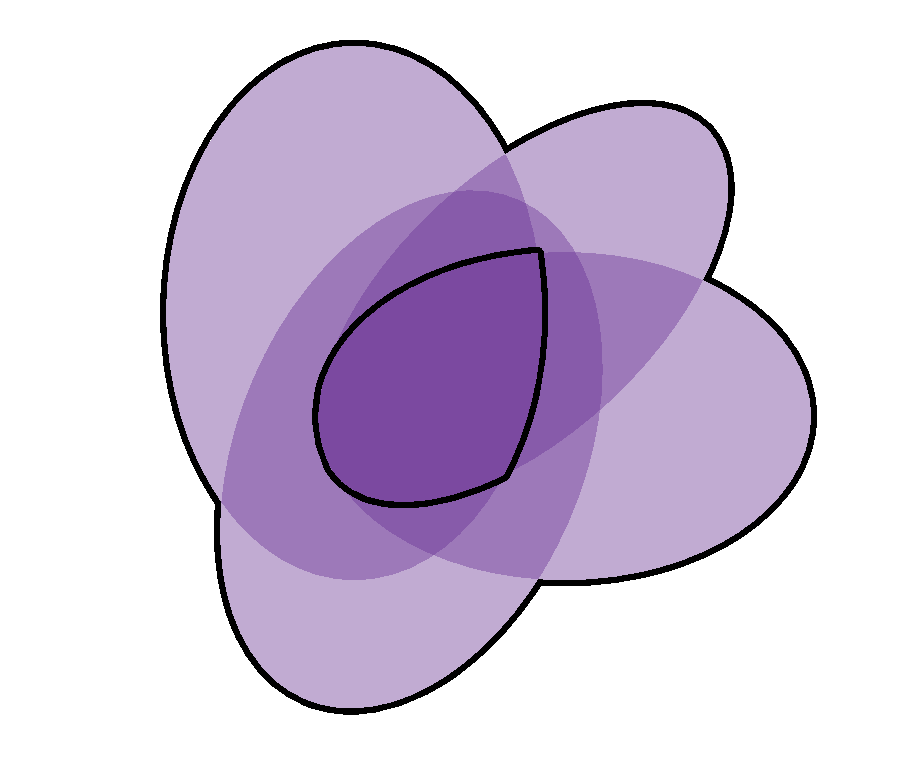
\includegraphics[scale=.45]{assets/intro/venn-soundness-b.pdf}
    \caption{Mathematical ideals $Any(P)$ (union) and $All(P)$ (intersection)}
    \label{fig:soundness-b}
\end{subfigure}
\begin{subfigure}{.47\textwidth}
    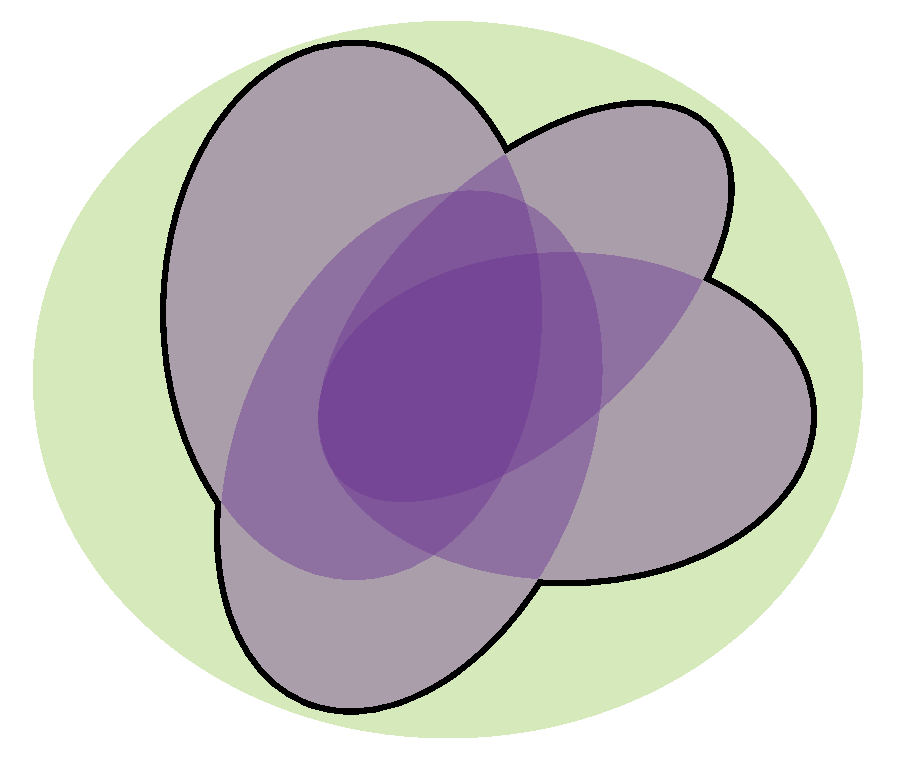
\includegraphics[scale=.45]{assets/intro/venn-soundness-c.pdf}
    \caption{Any sound-may analysis (green) in relation to $Any(P)$}
    \label{fig:soundness-c}
\end{subfigure}
\hfill
\begin{subfigure}{.47\textwidth}
    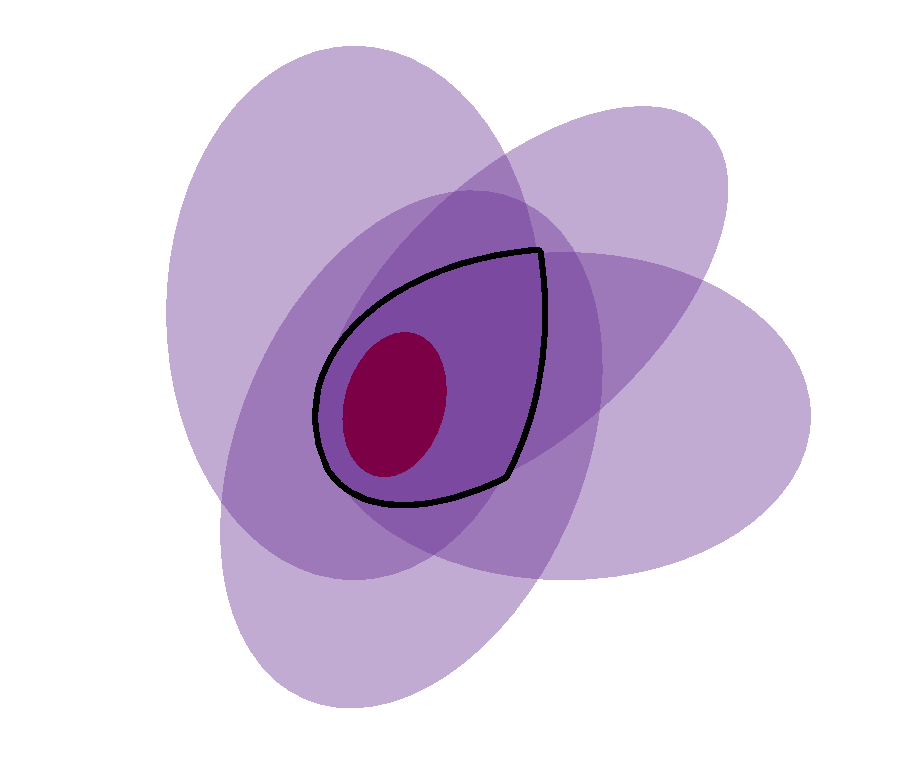
\includegraphics[scale=.45]{assets/intro/venn-soundness-d.pdf}
    \caption{Any sound-must analysis (red) in relation to $All(P)$}
    \label{fig:soundness-d}
\end{subfigure}
\begin{subfigure}{.47\textwidth}
    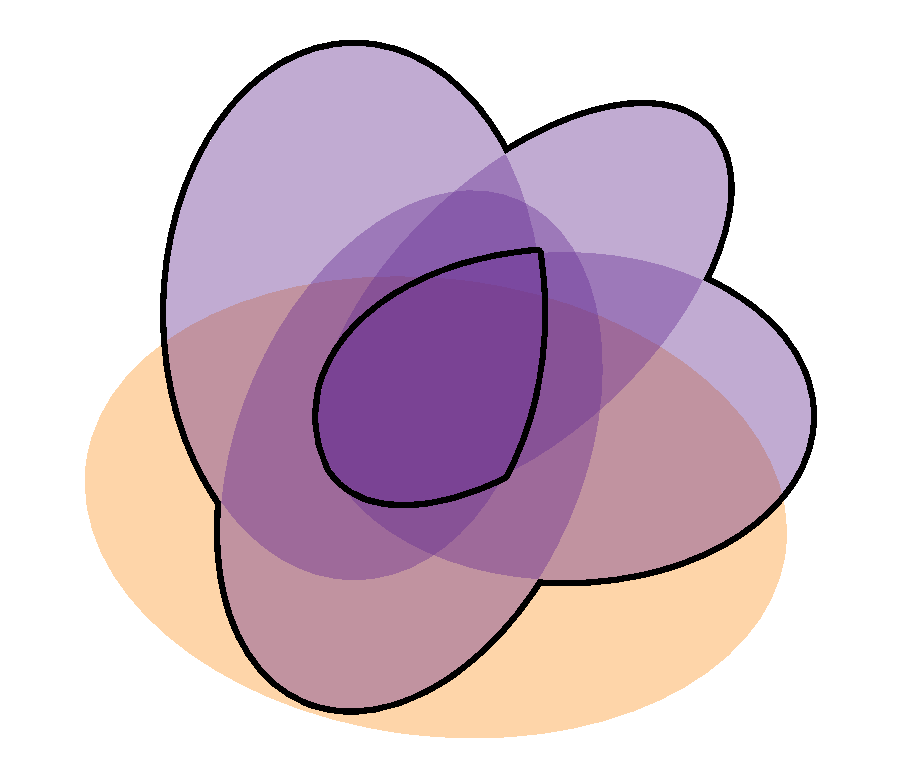
\includegraphics[scale=.45]{assets/intro/venn-soundness-e.pdf}
    \caption{Any unsound analysis (orange) in relation to both ideals}
    \label{fig:soundness-e}
\end{subfigure}
\hfill
\begin{subfigure}{.47\textwidth}
    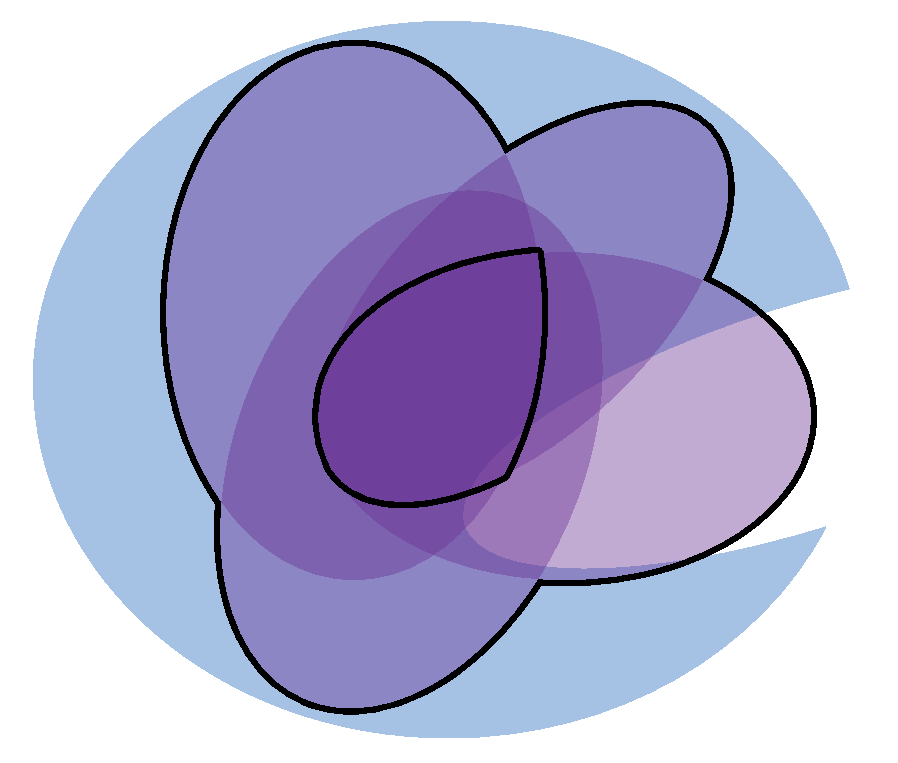
\includegraphics[scale=.45]{assets/intro/venn-soundness-f.pdf}
    \caption{Any \emph{soundy} analysis (blue) in relation to both ideals}
    \label{fig:soundness-f}
\end{subfigure}
\caption{Venn diagrams visualizing the relations of different static program analysis flavors to each other and to real behaviors}
\label{fig:soundness}
\end{figure}

Figure \ref{fig:soundness} attempts to shed some light on how different kinds
of static program analysis relate to each other and to the mathematical ideals.
Each set in figure \ref{fig:soundness-a} represents all behaviors exhibited
under a single actual program execution. Any static program analysis will
collapse different executions into a single set and will make claims about the
given program in general. In figure \ref{fig:soundness-b}, the ideal $Any(P)$
is represented by the union of all sets and that of $Any(P)$ by the
intersection, respectively. Any sound-may analysis will result in a superset of
$Any(P)$ (figure \ref{fig:soundness-c}), whereas any sound-must analysis will
result in a subset of $All(P)$ (figure \ref{fig:soundness-d}). Finally, any
unsound analysis (figure \ref{fig:soundness-e}) will result in a set with no
apparent properties; not entirely covering its appropriate mathematical ideal
but also including unrelated elements. More specifically though, as illustrated
in figure \ref{fig:soundness-f}, a soundy analysis will result in a set that
starts as a superset of $Any(P)$ but misses some hard (i.e., costly) to
overapproximate behaviors in well-known cases.


\section{Scientific Contributions}

In this section, we will briefly explain the main scientific contributions of
this dissertation. The exploration happens in the context of analyzing Java
programs \footnote{More specifically, the soon-to-be presented algorithms
operate on Java Bytecode --the lower-level intermediate representation used in
the Java Virtual Machine-- and thus they could, in theory, be applied to any
programming language that targets the Java VM.}, although it is not that
far-fetched to generalize results to other languages that offer similar
features. Additionally, most of our following contributions are expressed and
evaluated as part of the \doop{} framework [..], which offers several analyses
targeting the Java bytecode using Datalog specifications.

Ever since the introduction of object-sensitivity by Milanova et al. [..],
there has been increasing evidence that it is the superior context choice for
programs expressed in object-oriented languages, yielding a high precision to
cost ratio. Such has been its success that in practice it has almost superseded
the use of more traditional call-site sensitive analyses, when focusing on
object-oriented languages. Nevertheless, a call-site sensitive analysis is not
always inferior as there are language features and code patterns that may
partially favor this kind of context abstraction.

Subsequently, one might consider an approach where both context flavors are
--naively-- combined in every program point with the goal of increasing the
precision of the end result. Truly, such a combination would bear some
precision benefits but in most cases it would be accompanied by an infeasibly
high and disproportionate cost.

\paragraphhead{First contribution.} Our first scientific contribution is a step towards a more sophisticated
handling aiming to achieve a beneficial combination of both context flavors. We
propose a \emph{hybrid} context flavor for defining a family of analyses where
classical contexts are mixed and combined only in those program points where it
is profitable for the analysis. The resulting selective combination of both
context kinds vastly outperforms not only analyses following the naive
non-selective combination approach, but also their ``normal'' object-sensitive
counterparts. This result holds for a large array of analyses (e.g.,
1-object-sensitive, 2-object-sensitive with a context-sensitive heap, etc.)
establishing a new set of performance/precision sweet spots.

\paragraphhead{Second contribution.} The second scientific contribution tries to tackle an oft-reported issue with
context-sensitive analyses, in that they mostly operate in two extremes: either
the analysis is precise enough that it manipulates only manageable sets of
data, and thus scales impressively well, or the analysis gets quickly derailed
at the first sign of --massive-- imprecision and becomes orders-of-magnitude
more expensive than would be expected given the program's size. Currently,
there is no approach for a \emph{precise} context-\emph{sensitive} (of any
context flavor) analysis that would scale across the board at a level
comparable to that of a context-\emph{insensitive} one. Instead, we propose a
two step process by means of \emph{introspective analysis}: the approach
uniformly scales context-sensitive analyses by eliminating the
performance-detrimental behavior, only at a small precision expense.

Introspective analysis employs a common adaptive pattern: it first performs a
context-insensitive analysis and then it uses the results to selectively refine
(i.e., analyze context-sensitively) only those program elements that are
expected not to cause an explosion in running time or memory space. The
technical challenge is to appropriately identify such program elements. We show
that a simple but principled approach can be remarkably effective, achieving
scalability (often with dramatic speedup) for benchmarks previously completely
out-of-reach for deep context-sensitive analyses.

For the last two contributions, we shift our attention towards analyses that
aim for the highest confidence in their claims. Although quite reluctant and
conservative in making a claim, when they actually do they make certain that it
is the correct decision.

\paragraphhead{Third contribution.} The next, third contribution features a different flavor of static program
analysis. Instead of the more commonly researched paradigm of
\emph{may}-analyses, we chose to explore the alternative approach of a
\emph{must}-analysis. More specifically, we focus on an instance of a
\emph{must-alias} (also known as \emph{definite-alias}) analysis that aims to
infer aliasing relationships among program expressions that are guaranteed to
always hold. \footnote{As previously mentioned, a must-analysis will aim to
compute an underapproximation of behaviors that will happen in every possible
program execution.} The applications of a must-alias analysis are manifold:
\begin{inparaenum}[(1)]
\item it is useful for enabling optimizations such as constant folding and
	register allocation,
\item it can increase the precision of bug detectors, e.g. greatly benefiting a
	null-reference detector and a non-termination detector [..], and
\item it can be used internally as part of more complex analyses, e.g. one that
	can reason correctly about ``strong-updates'' at instructions that modify
	the heap.
\end{inparaenum}

Our proposed modeling is \emph{declarative}, expressed in the Datalog language
and thus it has the side effect of being executable out-of-the-box. In order to
compute high-confident results that at the same time are non-trivial, the
analysis needs to be flow-sensitive, i.e., compute information at each program
point and propagate it forward while respecting the control-flow of the
program.

Furthermore, we observe that a must-alias analysis exhibits certain properties
that can be exploited in order to achieve a more efficient algorithm without
any compromise in the precision or the validity of its results. We present a
custom specialized \emph{data structure} that speeds up a must-alias analysis
by nearly two orders of magnitude. The data structure achieves its efficiency
by encoding multiple alias sets in a single linked structure, and compactly
representing the aliasing relations of arbitrarily long program expressions.
Under this approach, must-alias analysis can be performed efficiently, over
large Java benchmarks, in under half a minute, making the analysis cost
acceptable for most practical uses.

\paragraphhead{Fourth contribution.} For our last contribution, we revisit the setting of a may-analysis but this
time while aiming to explore the potential of a truly \emph{sound} --instead of
just soundy-- yet \emph{practical} analysis. We present such an approach in a
\emph{defensive} may-points-to analysis, which can guarantee soundness even in
the presence of arbitrary opaque code \footnote{Code that cannot be analyzed
such as dynamically generated or native code, or dynamic language features such
as reflection, \code{invokedynamic}, etc.}. A key design tenet of our approach
is \emph{laziness}: the analysis computes points-to relationships only for
program expressions that are guaranteed to never escape into opaque code.

The defensive nature of our analysis means that it might miss some valid
inferences, but because of its laziness it will never waste work to compute
sets that are not ``complete'', i.e. that may be missing elements due to opaque
code. This frugal approach is what enables the great efficiency of our
algorithm, allowing for a highly precise points-to analysis (such as a
5-call-site-sensitive, flow-sensitive analysis). Despite its conservative
nature, our analysis yields sound, actionable results for a large subset of the
program code, achieving (under worst-case assumptions) 34-74\% of the program
coverage of an unsound state-of-the-art analysis for real-world programs.


\section{Outline}

The rest of this dissertation is organized as follows:
\begin{itemize}[$\bullet$]
\item Chapter~\ref{chapter:hybrid} examines how a naive combination of object
	sensitivity and call-site sensitivity into a single analysis can be
	massively penalizing in terms of performance. Following that, we
	presents a hybrid context-sensitive approach for implementing points-to
	analyses that leverage the benefits of combining both object- and a
	call-site- sensitivity while avoiding to pay most of the cost of a
	naive combination.

	This chapter presents research previously published in...

\item Chapter~\ref{chapter:introspective} examines a well-known bi-modal nature
	of classical static program points-to analyses in regards to scalability;
	they are either quite scalable or not scalable at all. In order to
	counter that discrepancy, we propose an adaptive approach in
	introspective analysis, where an imprecise analysis is used as a
	stepping stone in order to fine-tune program points in which a more
	precise handling is both beneficial and not detrimental to the overall
	analysis's performance.

	This chapter presents research previously published in...
\end{itemize}

Both aforementioned contributions aim for more scalable analyses that achieve
superior performance without foregoing precision. The next three contributions
aim for analyses that although more restrained on what they report, they do so
with much more confidence in the accuracy of their claims.

\begin{itemize}[$\bullet$]
\item Chapter~\ref{chapter:must-logic} examines how to compose a declarative
	model of a rich family of must-alias analyses, with emphasis on a careful
	and compact modeling, while at the same time exposing the key points
	where the algorithm's inference power can be adjusted.

	This chapter presents research previously published in...

\item Chapter~\ref{chapter:must-data} builds upon the previous chapter and goes
	forth to provide a specialized data structure that by exploiting the nature
	of a must-alias analysis it achieves high performance without any
	sacrifice on the accuracy of its results. We explore the data
	structure's performance in both an imperative (implemented in Java) and
	a declarative (implemented in Datalog) setting and contrast it
	extensively with prior techniques.

	This chapter presents research previously published in...

\item Chapter~\ref{chapter:defensive} examines how a defensive reasoning in the
	presence of opaque code can be combined along with computational laziness
	in order to produce a highly efficient, highly precise and truly sound
	may-points-to analysis.

	This chapter presents research previously published in...
\end{itemize}

\begin{itemize}[$\bullet$]
\item Chapter~\ref{chapter:panda} bla bla (paNda?)

\item Chapter~\ref{chapter:related} first discusses related work that is
	specific to previous chapters, and then expands to various other
	interesting subjects in the broader realm of static analysis.

\item Chapter~\ref{chapter:conclusions} concludes this dissertation by
	assessing our initial thesis and discussing future work.
\end{itemize}


\part{Achieving Scalability}
\chapter{Hybrid-Context Sensitivity}
\label{chapter:hybrid}
\epigraph{If you wanted to know about the Hybrid, why didn’t you just ask me?}{\textit{The 12th Doctor} - Doctor Who}

Although in principle call-site and object sensitivity are incomparable, in practice the story is quite clear. Call-site sensitivity has a long history, dating back to at least the '80s. For a long time, call-site sensitivity was considered synonymous with context sensitivity as a whole. Object sensitivity was later introduced in 2002 \cite{issta:2002:Milanova} and within a decade it has become the overwhelming choice of context sensitivity for object-oriented programs. Multiple studies \cite{pldi:2006:Naik,paste:2005:Liang,thesis:Lhotak,article:2008:tosem:Lhotak,oopsla:2009:Bravenboer} have found object-sensitive analyses to yield excellent precision/cost tradeoffs. Compared to call-site-sensitive analyses, an object-sensitive analysis of the same context depth has always been advantageous, in terms of both speed and performance.

Given such past experimental results, it would seem that exploring combinations of call-site and object sensitivity is futile. There is no tradeoff to exploit. Even though call-site-sensitive analyses are occasionally faster to execute, this only comes at the expense of precision. To achieve the same precision level as an object-sensitive analysis, call-site-sensitive analyses have to suffer much higher cost. Additionally, coarser approximations of object sensitivity, such as type sensitivity \cite{popl:2011:Smaragdakis} have filled the performance gap and offered fast options for cases when a full object-sensitive analysis is too expensive.

The question behind this chapter is whether the two kinds of context can be fruitfully combined, given how dissimilar they are. In order to address this question, we map the design space of \emph{hybrid} call-site- and object-sensitive analyses and describe the combinations that arise. Our work shows that the aforementioned conventional wisdom is false. This is one of the rare occasions when the combination of two ideas supplants both: hybrid-context sensitivity outperforms both object and call-site sensitivity in both precision and speed.

Naive hybrid combinations, such as always maintaining as context \emph{both} call and allocation sites, do not pay off, due to extremely high cost. For instance, keeping one call-site and one allocation site as context, in all places, yields a very expensive analysis, on average 3.9x slower than a simple 1-object-sensitive analysis. Although such a combination will improve precision, it is still lacking in comparison to, for example, a 2-object-sensitive analysis.

However, we find that more sophisticated hybrids are highly beneficial. Specifically, we show that we can switch per-language-feature between a combined context and an object-only context. For instance, contexts for static method calls are computed differently from contexts for dynamic method calls. This approach yields analyses with both low cost and high precision. Furthermore, adapting contexts per program feature defines a complex design space and allows even further optimization. Design choices arise, such as, how should the context adapt when a dynamic method call, or an object allocation are made inside a static method?

The end result is analyses that closely track the precision of a combined call-site-and-object sensitivity while incurring none of the cost. In fact, the cost of the resulting analysis is usually \emph{less} (and occasionally much less) than that of just an object-sensitive analysis, due to increased precision. This effect is shown to apply widely, to several variants of analyses. Accordingly, this outcome establishes new sweet spots for the analyses most relevant for practical applications: 1-object-sensitive, 2-object-sensitive with a 1-context-sensitive heap, and analogous type-sensitive \cite{popl:2011:Smaragdakis} analyses. For all of them, a selective hybrid context is typically both more precise and faster than the original analysis.

In all, this chapter describes the following contributions:

\begin{itemize}
\item We introduce the idea of hybrid call-site and object sensitivity where the two kinds of context are freely mixed and the mix is adjusted in response to analyzing different program features. The goal is to achieve the precision of keeping \emph{both} kinds of context together, but at the same cost as keeping only one.

\item We implement our approach in the \doop{} framework and apply it to a large variety of algorithms with varying context depth.

\item We show experimentally, over large Java benchmarks and the Java JDK, that hybrid-context sensitivity works remarkably well. Our experiments establish that different programming language constructs are best analyzed with different kinds of context. The selective application of a combined context achieves the same \emph{effective} precision as keeping both contexts at all times, at a fraction of the cost, and is typically faster even than keeping only an object context. For instance, in the practically important case of a 2-object-sensitive analysis with a context-sensitive heap, we get an average speedup of \nums{1.53x} \emph{and} a more precise analysis. Similarly, for the simple and popular 1-object-sensitive analysis, we get an average speedup of \nums{1.12x} combined with significant increase in precision.
\end{itemize}


\section{Hybrid-Context-Sensitive Analyses}
\label{sec:hybrid:main}

We can now explore interesting combinations of call-site and object sensitivity. The design space is large and we will be selective in our presentation and later experiments. Our choice of analyses in this space leverages insights from past studies on what kinds of context are beneficial.\footnote{We have validated these insights with extensive measurements on our experimental setup, and have generally explored a much larger portion of the design space than is possible to present in our evaluation section.} Such insights include:

\begin{itemize}
\item A call-site-sensitive heap is far less attractive than an object-sensitive heap. Generally, adding a heap context to a call-site-sensitive analysis increases precision very slightly, compared to the overwhelming cost.

\item When there is a choice between keeping an object-context or a call-site-context, the former is typically more profitable. This is well validated in extensive past measurements by Lhot\'{a}k and Hendren~\cite{article:2008:tosem:Lhotak}, comparing call-site-sensitive and object-sensitive analyses of various depths. In other words, call-site sensitivity is best added as \emph{extra} context over an object-sensitive analysis and will almost never pay off as a replacement context, for an object-oriented language.
\end{itemize}


\subsection{Uniform Hybrid Analyses}

The first kind of context combination is a straightforward one: both kinds of context are kept. We term such combinations \emph{uniform hybrid analyses}. In the variants we describe, a uniform hybrid analysis is guaranteed to be more precise\footnote{We use the term ``more precise'' colloquially. Strictly speaking, the analysis is guaranteed to be ``at least as precise'' and not necessarily ``more''.} than the base analysis being enhanced. The question is whether such precision will justify the added cost.

The insight is that by using every information available at each point we can get more precise analyses. Although that is proved to be true, experimental results also show that this precision gain comes with an infeasibly high cost in most cases. Still, we present some analyses that fully combine call-site and object sensitivity as a middle step for understanding later improvements and also as a baseline when comparing more elaborate ways of context combination.

\paragraph[Uniform 1-object-sensitive]{Uniform 1-object-sensitive hybrid (U-1obj).}
Enhancing a 1-object-sensitive analysis with call-site sensitivity results in an analysis with an empty heap context (\args{HC} = \args{\{$\star$\}}) but with a context that consists of both the allocation site of the receiver object and the invocation site of the method (\args{C} = \args{H $\times$ I}). The following definitions describe the analysis:

\begin{quote}
\cons{Record}{heap, ctx}{$\star$} \\
\cons{Merge}{heap, hctx, invo, ctx}{\bl{pair}(heap, invo)} \\
\cons{MergeStatic}{invo, ctx}{\bl{pair}(\bl{first}(ctx), invo)} 
\end{quote}

In words: a virtual method has as context the abstraction of its receiver object, extended with the method's invocation site.  A static method keeps a context consisting of the most significant part of the caller's context and the method's invocation site. Note that under the above definitions, the context of a U-1obj analysis is always a superset of that of 1obj, hence the analysis is strictly more precise.

\paragraph[Uniform 2-object-sensitive with 1-context-sensitive heap]{Uniform 2-object-sensitive with 1-context-sensitive heap hybrid (U-2obj+H).}
A 2-object-sensitive analysis with a context-sensitive heap can be enhanced in the same way. A heap context consists of an allocation site (\args{HC} = \args{H}) and a method context consists of two allocation sites and one invocation site (\args{C} = \args{H $\times$ H $\times$ I}).  The constructor definitions for the analysis are:

\begin{quote}
\cons{Record}{heap, ctx}{\bl{first}(ctx)} \\
\cons{Merge}{heap, hctx, invo, ctx}{\bl{triple}(heap, hctx, invo)} \\
\cons{MergeStatic}{invo, ctx}{\bl{triple}(\bl{first}(ctx), \bl{second}(ctx), invo)} 
\end{quote}

In words: an object's heap context is the receiver object of the method doing the allocation. A virtual method's context is its receiver object's allocation site and context (the latter being the allocation site of the object that allocated the receiver), followed by the invocation site of the method. On a static call, the heap part (i.e., first two elements) of the method context is kept unchanged, and extended with the invocation site of the call.

This analysis is also strictly more precise than the ``plain'' analysis it is based on, 2obj+H. This is achieved partly by placing the receiver object's allocation site in the most significant position of the context triple. In this way, the \consname{Record} function produces the same heap context as 2obj+H on an object's allocation. Alternative definitions are possible for the same sets of contexts, \args{C} and \args{HC}. For instance, one could choose to place \args{hctx} in the most significant position. Similarly, one could produce a hybrid analysis based on 2obj+H but with a different kind of heap context, e.g., \args{HC} = \args{I}, therefore using the invocation site in a method's context as an allocation context. These definitions make decisively less sense, however, per the insights mentioned earlier: invocation sites are rarely advantageous as heap contexts, and, similarly, it is not reasonable to invert the natural significance order of \args{heap} vs. \args{hctx}. (We have also verified experimentally that such combinations yield bad analyses.)

Note here that in deeper analyses where some elements from the context are used in order to create new heap contexts, it is important which ones we choose to propagate. Different choices might result in analyses that behave quite differently both in terms of performance and precision. We can easily influence which context elements are selected for propagation, by changing their ordering in the context.

\paragraph[Uniform 2-type-sensitive with 1-context-sensitive heap]{Uniform 2-type-sensitive with 1-context-sensitive heap hybrid (U-2type+H).}
Isomorphically to object sensitivity, we can enhance type-sensitive analyses with call-site information in the same way. When applied to a 2-type-sensitive analysis with a context-sensitive heap, this results in an analysis with a heap context of one type (\args{HC} = \args{T}) and a context of two types and an invocation site (\args{C} = \args{T $\times$ T $\times$ I})---mirroring the 2-object-sensitive analysis with a context sensitive heap. The definitions are almost identical:

\begin{quote}
\cons{Record}{heap, ctx}{\bl{first}(ctx)} \\
\cons{Merge}{heap, hctx, invo, ctx}{\bl{triple}($\mathcal{C_A}$(heap), hctx, invo)} \\
\cons{MergeStatic}{invo, ctx}{\bl{triple}(\bl{first}(ctx), \bl{second}(ctx), invo)} 
\end{quote}


\subsection{Selective Hybrid Analyses}

Another approach to hybrid call-site- and object-sensitive analyses is to maintain a context that varies inside the same analysis. We call such analyses \emph{selective hybrid analyses}, as opposed to the earlier ``uniform hybrid'' ones. In a selective hybrid analysis, the sets of contexts, \args{C} and \args{HC}, will be formed as the cartesian product of unions of sets. Depending on the information available at different analysis points where new contexts are formed, we shall create contexts of a different kind, instead of always keeping a combination of rigid form. We have already hinted at such opportunities in Section~\ref{sec:back:model-instances}: at a static method call, an object-sensitive analysis does not have a heap object available to create a new context, hence it can at best propagate the context of the caller. Yet, an invocation site is available and can be used to distinguish different static calls, as long as we are allowed to use it as context. This observation generalizes: static invocations are a language feature that benefits highly from the presence of call-site-sensitive elements in the context. This is not hard to explain: For object-sensitive analyses, when analyzing a static invocation, we do not have much information to use in creating a new context, in contrast to a ``normal'' virtual invocation. Consequently, it is beneficial to be able to use the invocation site as a differentiator of static calls.

Selective hybrid analyses are among the most interesting parts of our work and, to our knowledge, have never before arisen in the literature, far less specified, implemented, and evaluated.

\paragraph[Selective 1-object-sensitive (-A)]{Selective 1-object-sensitive hybrid A (S$_A$-1obj).}
Trying to selectively enhance a 1-object-sensitive analysis (\args{HC} = \args{\{$\star$\}}) with call-site sensitive elements, we are presented with two options, relative to how contexts are created in static invocations. The first option is quite simple: we can keep only a single context element in both virtual and static invocations. Consequently, in virtual invocations the context will be an allocation site, but in static invocations it will be an invocation site (\args{C} = \args{H $\cup$ I}). The definitions needed are the following:

\begin{quote}
\cons{Record}{heap, ctx}{$\star$} \\
\cons{Merge}{heap, hctx, invo, ctx}{heap} \\
\cons{MergeStatic}{invo, ctx}{invo} 
\end{quote}

Note that this analysis is \emph{not} guaranteed to be more precise than the 1obj analysis it is based on. Nevertheless, it should be an excellent reference point for comparison and insights: it will suggest how much precision can be gained or lost by call-site sensitivity as a replacement of object sensitivity in static method calls.

\paragraph[Selective 1-object-sensitive (-B)]{Selective 1-object-sensitive hybrid B (S$_B$-1obj).}
The second option for a selective hybrid enhancement of a 1-object-sensitive analysis is to add extra information to the context of static calls. This means that context in virtual invocations is still an allocation site, but context in static invocations now consists of both the allocation site copied from the caller \emph{and} the invocation site. In this way, \args{C} = \args{H $\times$ (I $\cup$ \{$\star$\})}. That is, the context can be either just an allocation site or an allocation site and an invocation site. (This could also be written equivalently as \args{C} = \args{H $\cup$ (H $\times$ I)}, but the earlier form streamlines the definitions of constructors, as it makes all contexts be pairs, thus avoiding case-based definitions.)  In this way the constructor definitions become:

\begin{quote}
\cons{Record}{heap, ctx}{$\star$} \\
\cons{Merge}{heap, hctx, invo, ctx}{\bl{pair}(heap, $\star$)} \\
\cons{MergeStatic}{invo, ctx}{\bl{pair}(\bl{first}(ctx), invo)}
\end{quote}

This analysis has a context that is always a superset of the 1obj context and, therefore, is guaranteed to be more precise.

\paragraph[Selective 2-object-sensitive with 1-context-sensitive heap]{Selective 2-object-sensitive with 1-context-sensitive heap hybrid (S-2obj+H).}
When dealing with deeper analyses, the possible design decisions start to vary. For example, for a 2-object-sensitive analysis with a context-sensitive heap, an interesting choice is to have allocation sites as heap contexts (\args{HC} = \args{H}), and for method contexts to keep standard object-sensitive information for virtual calls but favor call-site sensitivity for static calls. The constructor definitions for the above analysis are:

\begin{quote}
\cons{Record}{heap, ctx}{\bl{first}(ctx)} \\
\cons{Merge}{heap, hctx, invo, ctx}{\bl{triple}(heap, hctx, $\star$)} \\
\cons{MergeStatic}{invo, ctx}{\bl{triple}(\bl{first}(ctx), invo, \bl{second}(ctx))} 
\end{quote}

(In this way, we have \args{C} = \args{H $\times$ (H $\cup$ I) $\times$ (H $\cup$ I $\cup$ \{$\star$\})}.) Note the interesting behavior of such an analysis: for virtual calls, the context is equivalent to that of 2obj+H. For the first static call (i.e., from inside a virtually called method), the context is a superset of 2obj+H, augmented by an invocation site. For further static calls (i.e., static calls inside statically called methods), however, the analysis favors call-site sensitivity (both the last two elements of context are invocation sites) and otherwise only remembers the most-significant element of the object-sensitive context. (The latter is important for creating high-quality heap contexts, when allocating objects.) It is interesting to see how this analysis fares relative to 2obj+H, since the analyses are in principle incomparable in precision.

\paragraph[Selective 2-type-sensitive with 1-context-sensitive heap]{Selective 2-type-sensitive with 1-context-sensitive heap hybrid (S-2type+H).}
Finally, type-sensitive analyses can be enhanced with call-site sensitive information in much the same way. Mirroring our choices in S-2obj+H, the S-2type+H analysis has heap context \args{HC} = \args{T} and method context \args{C} = \args{T $\times$ (T $\cup$ I) $\times$ (T $\cup$ I $\cup$ \{$\star$\})}. The constructor definitions are isomorphic to the S-2obj+H analysis:

\begin{quote}
\cons{Record}{heap, ctx}{\bl{first}(ctx)} \\
\cons{Merge}{heap, hctx, invo, ctx}{\bl{triple}($\mathcal{C_A}$(heap), hctx, $\star$)} \\
\cons{MergeStatic}{invo, ctx}{\bl{triple}(\bl{first}(ctx), invo, \bl{second}(ctx))} 
\end{quote}

\paragraph[Other analyses]{Other analyses.}
The above discussion does not nearly exhaust the space of hybrid combinations. Consider selective hybrids for a 2obj+H analysis: Many more design choices are possible than the one shown. One could change the heap context into an invocation site, or into a union of invocation and call-site (\args{HC} = \args{H $\cup$ I}). This combination is a bad choice, due to the poor payoff of call-site heap contexts. One could create context structures that let call-site- and object-sensitive context elements freely merge, e.g., \args{C} = \args{(H $\cup$ I) $\times$ (H $\cup$ I) $\times$ (H $\cup$ I $\cup$ \{$\star$\})}. This allows several different definitions of context constructors, but has the drawback of diverging significantly from object sensitivity (i.e., allowing to skip even the most-significant, object-sensitive context element), which misses the well documented precision and performance advantages of object sensitivity, especially as a heap context.


\section{Evaluation}
\label{sec:evaluation}

We implemented and evaluated all aforementioned analyses using the \doop{} framework. There are interesting and subtle aspects in our measurements, but the executive summary is clear: uniform hybrid analyses are typically not good choices in practice: their precision is offset by a very high performance cost. A relative exception is the uniform type-sensitive hybrid analysis, U-2type+H, which, although higher-cost, is not prohibitively expensive and offers a reasonable precision/performance tradeoff.  Selective hybrid analyses, on the other hand, are not just interesting tradeoffs but clear winners: they match or (usually) outperform the object-sensitive analyses they are based on, while offering better precision, closely approaching the precision of the much more costly uniform hybrids. Overall, the best analyses in our evaluation set, both for highest-precision and for high performance with good precision, are selective hybrids.

Our evaluation setting uses the LogicBlox Datalog engine, v.3.9.0, on a Xeon X5650 2.67GHz machine with only one thread running at a time and 24GB of RAM (i.e., ample for the analyses studied). We analyze the DaCapo benchmark programs (v.2006-10-MR2) under JDK 1.6.0\_37. This is a much larger set of libraries than earlier work~\cite{oopsla:2009:Bravenboer,popl:2011:Smaragdakis}, which also results in differences in measurements, since the numbers shown integrate application- and library-level metrics. All runtime numbers are medians of three runs. As in other published work~\cite{popl:2011:Smaragdakis,ecoop:2012:Ali}, jython and hsqldb are analyzed with reflection disabled and hsqldb has its entry point set manually in a special harness.

\begin{figure*}[tb!p]
\begin{center}
\begin{subfigure}[b]{0.45\textwidth}
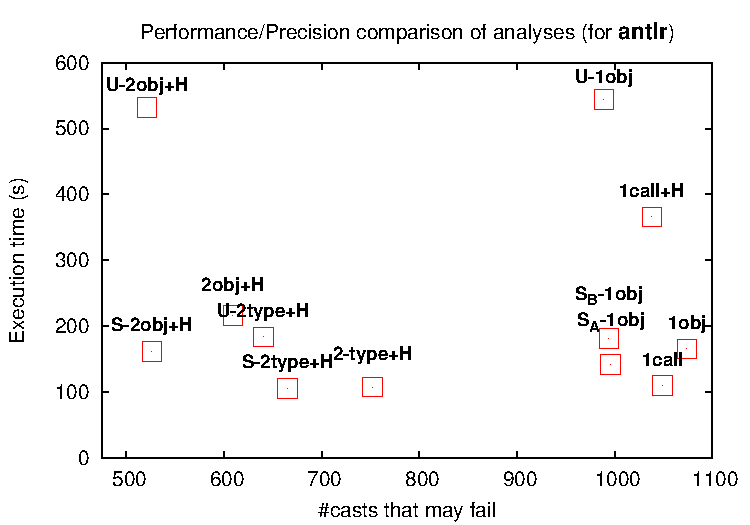
\includegraphics[width=\textwidth]{assets/hybrid/antlr.pdf}
\end{subfigure}\hspace{1cm}%
\begin{subfigure}[b]{0.45\textwidth}
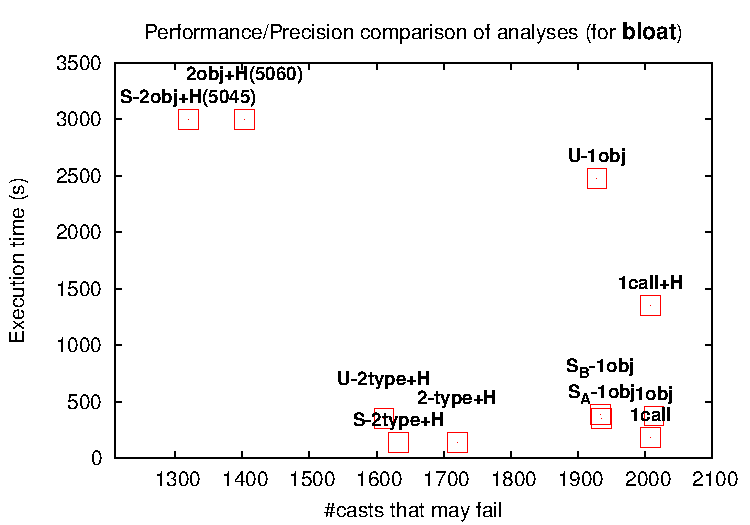
\includegraphics[width=\textwidth]{assets/hybrid/bloat.pdf}
\end{subfigure}

\begin{subfigure}[b]{0.45\textwidth}
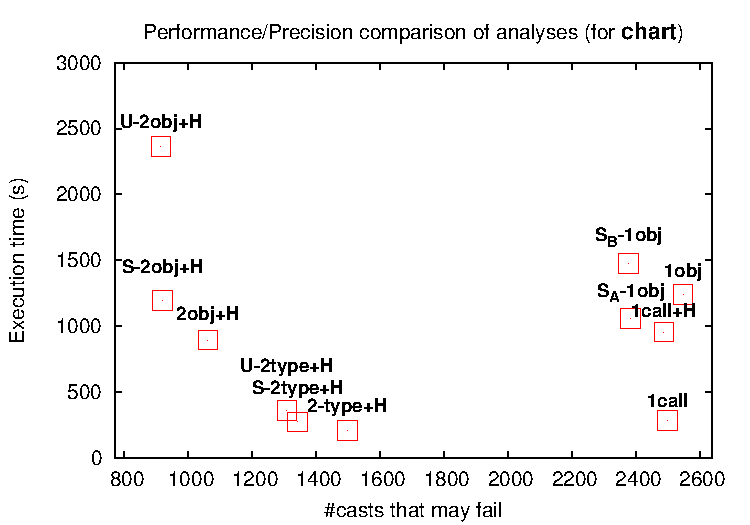
\includegraphics[width=\textwidth]{assets/hybrid/chart.pdf}
\end{subfigure}\hspace{1cm}%
\begin{subfigure}[b]{0.45\textwidth}
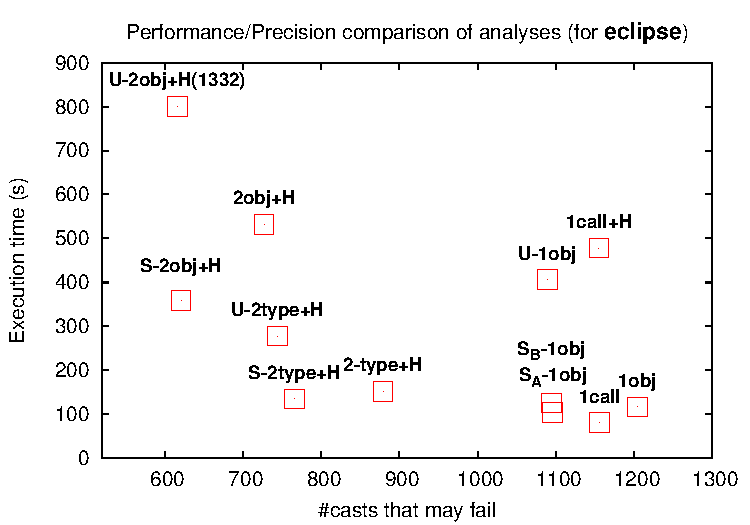
\includegraphics[width=\textwidth]{assets/hybrid/eclipse.pdf}
\end{subfigure}

\begin{subfigure}[b]{0.45\textwidth}
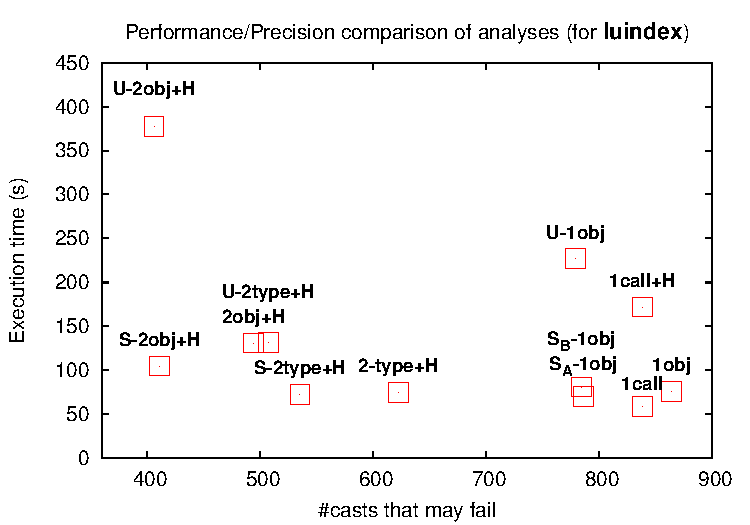
\includegraphics[width=\textwidth]{assets/hybrid/luindex.pdf}
\end{subfigure}\hspace{1cm}%
\begin{subfigure}[b]{0.45\textwidth}
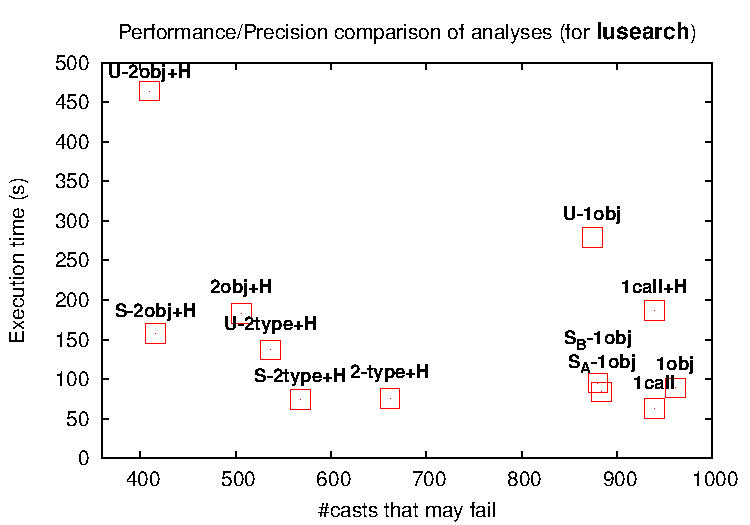
\includegraphics[width=\textwidth]{assets/hybrid/lusearch.pdf}
\end{subfigure}

\begin{subfigure}[b]{0.45\textwidth}
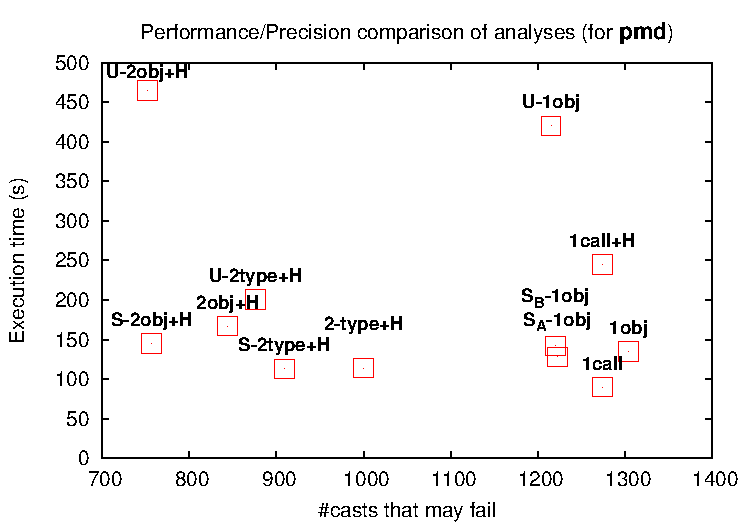
\includegraphics[width=\textwidth]{assets/hybrid/pmd.pdf}
\end{subfigure}\hspace{1cm}%
\begin{subfigure}[b]{0.45\textwidth}
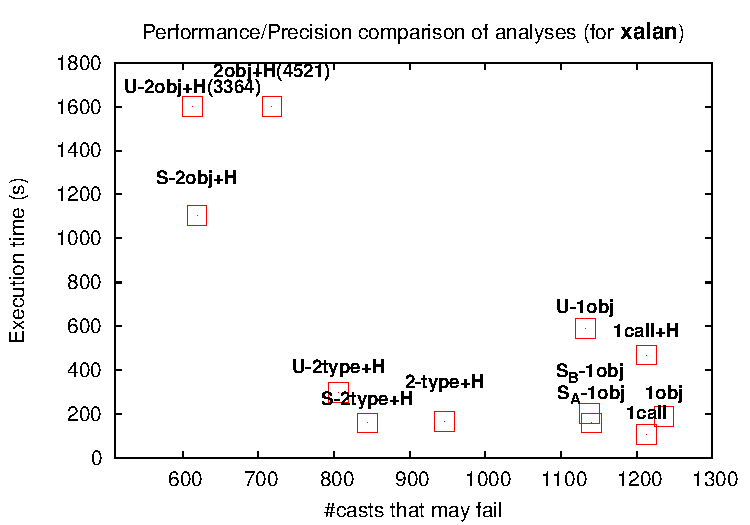
\includegraphics[width=\textwidth]{assets/hybrid/xalan.pdf}
\end{subfigure}
\caption{Graphical depiction of performance vs. precision metrics for eight of our benchmarks over all analyses. Lower is better on both axes. The Y axis is truncated for readability. Out-of-bounds points are included at lower Y values, with their real running time in parentheses.}
\label{fig:hybrid:precision}
\end{center}
\end{figure*}

For an illustration of the precision and performance spectrum, consider Figure~\ref{fig:hybrid:precision}, which plots analyses on precision/performance axes. The figure plots execution time against precision in the ``may-fail casts'' metric, i.e., the number of casts that the analysis cannot statically prove safe. Lower numbers are better on both axes, thus an analysis that is to the \textbf{left and below} another is better in both precision and performance. Values that are disproportionately high on the Y axis (i.e., large execution times) are clipped and plotted at the top of the figure, with the actual number included in parentheses. (Note that the Y axis starts at zero, while the X axis starts at an arbitrary point---we cannot know what is the ``ideal'' reference value for this metric.)

In terms of pre-existing analyses, Figure~\ref{fig:hybrid:precision} illustrates what has been past experience: 2obj+H is the most precise analysis, but often heavy. 1obj and 2type+H are both quite fast, with 2type+H also showing very good precision, often approaching 2obj+H. The two call-site-sensitive analyses (1call, 1call+H) are mostly shown for reference and to demonstrate the insights discussed in Section~\ref{sec:hybrid:main}. 1call is a fast analysis but vastly imprecise, while 1call+H is a bad tradeoff: its cost grows quite significantly relative to 1call without much precision added---call-site sensitivity is a bad choice for heap contexts.

As can be seen, the selective hybrid analyses (S$_A$-1obj, S$_A$-1obj, S-2obj+H, S-2type+H) usually offer an advantage over the corresponding base analysis (1obj, 2type+H, 2obj+H) in both precision and performance. In fact, selective hybrids are typically imperceptibly less precise than the corresponding uniform hybrid, yet much more precise than the base analysis. For instance, the plot points for S-2obj+H are always barely to the right of those for the theoretically more precise U-2obj+H (but significantly lower---uniform hybrids are very expensive), while they are clearly to the left of 2obj+H.


\subsection{Detailed Results}

Detailed results of our experiments are presented in Tables \ref{tab:hybrid:results-a} and \ref{tab:hybrid:results-b}. The tables show precision and performance metrics for all analyses. The precision metrics are:
\begin{inparaenum}[(1)]
\item the average points-to set size (i.e., average over all variables of their
points-to sets sizes),
\item the number of edges in the computed call-graph (which is typically a good proxy for the overall precision of the analysis, in broad strokes), and
the results of two client analyses:
\item the number of virtual calls that could not be de-virtualized, and
\item the number of casts that could not be statically proven safe.
\end{inparaenum}
A combination of these four metrics gives a reliable picture of the precision of an analysis. Note that the average points-to set size alone is not necessarily reliable, because it is influenced by a small number of library variables with enormous points-to sets. For comparison, the \emph{\textbf{median}} points-to set size is 1, for all analyses and benchmarks.

Performance is shown with two metrics:
\begin{inparaenum}[(1)]
\item time and
\item total size of all \emph{context-sensitive} points-to sets.
\end{inparaenum}
Although time is the ultimate performance metric, it is brittle: one can argue that our time measurements are influenced by a multitude of implementation or environment factors, among which are the choice of underlying data structures, indexing, and the overall implementation of the points-to analysis, especially since it is running on a Datalog engine, with its own complex implementation choices hidden. The context-sensitive points-to set size metric does not suffer from any such measurement or implementation bias. It is the foremost internal complexity metric of a points-to analysis, and typically correlates well with time, for analyses of the same flavor. Note that analysis implementations that fundamentally differ from ours also try hard to minimize this metric in order to achieve peak performance: Lhot\'{a}k's \textsc{Paddle} framework~\cite{thesis:Lhotak} is using binary decision diagrams (BDDs) for representing relations. The best BDD variable ordering (yielding ``impressive results'' \cite{pldi:2003:Berndl}) is one that minimizes the total size of context-sensitive points-to sets. In short, it is reasonable to expect that improvements in this internal metric reinforce the verdict of which analysis yields better performance, not just in our setting but generally. Furthermore, the size of context-sensitive points-to sets serves as a valuable indicator of the internally different computation performed by various analyses: Analyses with almost identical precision metrics (e.g., context-insensitive points-to set sizes, call-graph edges) have vastly different context-sensitive points-to set sizes.


\begin{table*}
\scalebox{0.8}{
\begin{tabular}{|r|c|l|p{1cm}|p{1cm}|p{1cm}!{\vrule width 2pt}l|l!{\vrule width 2pt}c|l|p{1cm}|p{1cm}|p{1cm}!{\vrule width 2pt}l|l|}

\cline{3-8}\cline{10-15}
\multicolumn{2}{c|}{} &
\rotatebox{90}{avg. objs per var} &
\rotatebox{90}{call-graph edges} &
\rotatebox{90}{polymorph v-calls} &
\rotatebox{90}{may-fail casts} &
\rotatebox{90}{elapsed time (s)} &
\rotatebox{90}{sensitive VPT (M)} &
\multicolumn{1}{c|}{} &
\rotatebox{90}{avg. objs per var} &
\rotatebox{90}{call-graph edges} &
\rotatebox{90}{polymorph v-calls} &
\rotatebox{90}{may-fail casts} &
\rotatebox{90}{elapsed time (s)} &
\rotatebox{90}{sensitive VPT (M)} \\

\cmidrule[2pt]{3-8}\cmidrule[2pt]{10-15}
\multicolumn{3}{c|}{} &
over 8.8K meths &
over 33K calls &
over 1.7K casts &
\multicolumn{4}{c|}{} &
over 10.2K meths &
over 31K calls &
over 2.8K casts &
\multicolumn{2}{c}{} \\
\cline{1-15}
1call & \multirow{13}{*}{\rotatebox{90}{\mbox{antlr}}} & 29.79 & 60999 & 1994 & 1049 & 110 & 16 & \multirow{13}{*}{\rotatebox{90}{\mbox{bloat}}} & 43.96 & 70506 & 2138 & 2008 & 186 & 32.9 \\
1call+H & & 29.58 & 60999 & 1994 & 1038 & 366 & 54.8 & & 43.94 & 70506 & 2138 & 2008 & 1351 & 150.5 \\
\cline{1-1}\cline{3-8}\cline{10-15}
1obj & & 24.86 & 60194 & 1933 & 1074 & 166 & 14.3 & & 41.26 & 69501 & 2076 & 2013 & 374 & 21.9 \\
U-1obj & & 24.55 & 60194 & 1933 & 989 & 544 & 65 & & 41.16 & 69501 & 2076 & 1928 & 2473 & 287.1 \\
S$_A$-1obj & & 24.90 & 60202 & 1936 & 996 & \best{142} & \best{10.5} & & 41.32 & 69511 & 2080 & 1935 & \best{353} & \best{20.1} \\
S$_B$-1obj & & 24.61 & 60194 & 1933 & 994 & 182 & 17.3 & & 41.18 & 69501 & 2076 & 1933 & 391 & 24 \\
\cline{1-1}\cline{3-8}\cline{10-15}
2obj+H & & 6.42 & 55548 & 1707 & 609 & 217 & 19.9 & & 13.25 & 60726 & 1640 & 1403 & 5060 & 153.5 \\
U-2obj+H & & 6.26 & 55548 & 1707 & 521 & 532 & 39.5 & & \bad{-} & \bad{-} & \bad{-} & \bad{-} & \bad{-} & \bad{-} \\
S-2obj+H & & 6.27 & 55548 & 1707 & 526 & \best{162} & \best{13.9} & & 13.10 & 60726 & 1640 & 1320 & \best{5045} & \best{149.8} \\
\cline{1-1}\cline{3-8}\cline{10-15}
2type+H & & 17.60 & 55850 & 1759 & 752 & 108 & 5.3 & & 16.28 & 62115 & 1888 & 1720 & 142 & 11.4 \\
U-2type+H & & 7.14 & 55765 & 1746 & 640 & 184 & 8.9 & & 14.71 & 61753 & 1827 & 1611 & 353 & 30.3 \\
S-2type+H & & 17.39 & 55850 & 1759 & 665 & \best{106} & \best{4.8} & & 16.10 & 62115 & 1888 & 1633 & \best{140} & \best{11} \\

\cmidrule[2pt]{1-15}
\multicolumn{3}{c|}{} &
over 15K meths &
over 35K calls &
over 3.5K casts &
\multicolumn{4}{c|}{} &
over 9.3K meths &
over 23K calls &
over 2K casts &
\multicolumn{2}{c}{} \\
\cline{1-15}
1call & \multirow{13}{*}{\rotatebox{90}{\mbox{chart}}} & 45.12 & 82156 & 2900 & 2500 & 288 & 49.6 & \multirow{13}{*}{\rotatebox{90}{\mbox{eclipse}}} & 21.84 & 53006 & 1515 & 1156 & 81 & 12.3 \\
1call+H & & 45.11 & 82078 & 2897 & 2488 & 957 & 120.9 & & 21.65 & 53001 & 1514 & 1155 & 478 & 61.5 \\
\cline{1-1}\cline{3-8}\cline{10-15}
1obj & & 40.80 & 81423 & 2821 & 2548 & 1240 & 62.5 & & 18.65 & 52114 & 1429 & 1204 & 117 & 9.4 \\
U-1obj & & \bad{-} & \bad{-} & \bad{-} & \bad{-} & \bad{-} & \bad{-} & & 18.41 & 51935 & 1404 & 1089 & 406 & 42.3 \\
S$_A$-1obj & & 40.72 & 81075 & 2815 & 2385 & \best{1059} & \best{39.7} & & 18.59 & 51958 & 1412 & 1096 & \best{105} & \best{7.6} \\
S$_B$-1obj & & 40.11 & 81012 & 2808 & 2378 & 1477 & 89.7 & & 18.43 & 51936 & 1404 & 1094 & 126 & 10.8 \\
\cline{1-1}\cline{3-8}\cline{10-15}
2obj+H & & 5.30 & 59162 & 1610 & 1062 & \best{896} & 67.6 & & 5.75 & 44900 & 1163 & 727 & 532 & 44.6 \\
U-2obj+H & & 4.99 & 59142 & 1603 & 915 & 2363 & 115.7 & & 5.60 & 44899 & 1163 & 616 & 1332 & 89.8 \\
S-2obj+H & & 5.00 & 59152 & 1610 & 920 & 1199 & \best{53} & & 5.61 & 44900 & 1163 & 621 & \best{359} & \best{32.3} \\
\cline{1-1}\cline{3-8}\cline{10-15}
2type+H & & 7.02 & 62290 & 1775 & 1498 & \best{211} & \best{13.3} & & 7.93 & 45318 & 1233 & 879 & 152 & 13.6 \\
U-2type+H & & 5.89 & 62172 & 1756 & 1309 & 362 & 21.3 & & 6.41 & 45123 & 1202 & 744 & 278 & 24.4 \\
S-2type+H & & 6.57 & 62280 & 1775 & 1343 & 276 & 16.5 & & 7.61 & 45235 & 1229 & 766 & \best{135} & \best{11.5} \\

\cmidrule[2pt]{1-15}
\multicolumn{3}{c|}{} &
over 10K meths &
over 26K calls &
over 2K casts &
\multicolumn{4}{c|}{} &
over 8.5K meths &
over 21K calls &
over 1.9K casts &
\multicolumn{2}{c}{} \\
\cline{1-15}
1call & \multirow{13}{*}{\rotatebox{90}{\mbox{hsqldb}}} & 18.56 & 54619 & 1552 & 1360 & 90 & 9.6 & \multirow{13}{*}{\rotatebox{90}{\mbox{jython}}} & 20.64 & 50494 & 1525 & 1140 & 88 & 10.4 \\
1call+H & & 18.53 & 54619 & 1552 & 1360 & 332 & 39.8 & & 20.57 & 50480 & 1524 & 1140 & 401 & 50.6 \\
\cline{1-1}\cline{3-8}\cline{10-15}
1obj & & 15.41 & 53726 & 1480 & 1385 & 218 & 13.9 & & 18.21 & 49622 & 1448 & 1157 & 119 & 8.7 \\
U-1obj & & 15.30 & 53724 & 1479 & 1302 & 1351 & 74.3 & & 18.01 & 49614 & 1448 & 1087 & 375 & 43.2 \\
S$_A$-1obj & & 15.58 & 53730 & 1482 & 1320 & \best{183} & \best{9.6} & & 18.19 & 49622 & 1453 & 1094 & 138 & \best{6.7} \\
S$_B$-1obj & & 15.32 & 53724 & 1479 & 1308 & 329 & 29.5 & & 18.09 & 49614 & 1448 & 1092 & 138 & 10.8 \\
\cline{1-1}\cline{3-8}\cline{10-15}
2obj+H & & \bad{-} & \bad{-} & \bad{-} & \bad{-} & \bad{-} & \bad{-} & & \bad{-} & \bad{-} & \bad{-} & \bad{-} & \bad{-} & \bad{-} \\
U-2obj+H & & \bad{-} & \bad{-} & \bad{-} & \bad{-} & \bad{-} & \bad{-} & & \bad{-} & \bad{-} & \bad{-} & \bad{-} & \bad{-} & \bad{-} \\
S-2obj+H & & \bad{-} & \bad{-} & \bad{-} & \bad{-} & \bad{-} & \bad{-} & & \bad{-} & \bad{-} & \bad{-} & \bad{-} & \bad{-} & \bad{-} \\
\cline{1-1}\cline{3-8}\cline{10-15}
2type+H & & 7.92 & 49421 & 1276 & 1031 & \best{195} & \best{13.7} & & 8.55 & 43269 & 1268 & 909 & 731 & \best{52} \\
U-2type+H & & 6.71 & 49319 & 1263 & 923 & 583 & 42.9 & & 7.18 & 43138 & 1236 & 822 & 1363 & 118.4 \\
S-2type+H & & 7.74 & 49421 & 1276 & 948 & 238 & 20.5 & & 8.30 & 43269 & 1268 & 840 & \best{676} & 56.5 \\
\cline{1-15}

\end{tabular}
} % end scalebox
\caption[]{Precision and performance metrics for all benchmarks and analyses, grouped by relevance. Continues in Table~\ref{tab:hybrid:results-b}.}
\label{tab:hybrid:results-a}
\end{table*}

\begin{table*}
\scalebox{0.8}{
\begin{tabular}{|r|c|l|p{1cm}|p{1cm}|p{1cm}!{\vrule width 2pt}l|l!{\vrule width 2pt}c|l|p{1cm}|p{1cm}|p{1cm}!{\vrule width 2pt}l|l|}

\cline{3-8}\cline{10-15}
\multicolumn{2}{c|}{} &
\rotatebox{90}{avg. objs per var} &
\rotatebox{90}{call-graph edges} &
\rotatebox{90}{polymorph v-calls} &
\rotatebox{90}{may-fail casts} &
\rotatebox{90}{elapsed time (s)} &
\rotatebox{90}{sensitive VPT (M)} &
\multicolumn{1}{c|}{} &
\rotatebox{90}{avg. objs per var} &
\rotatebox{90}{call-graph edges} &
\rotatebox{90}{polymorph v-calls} &
\rotatebox{90}{may-fail casts} &
\rotatebox{90}{elapsed time (s)} &
\rotatebox{90}{sensitive VPT (M)} \\

\cmidrule[2pt]{3-8}\cmidrule[2pt]{10-15}
\multicolumn{3}{c|}{} &
over 7.9K meths &
over 18K calls &
over 1.4K casts &
\multicolumn{4}{c|}{} &
over 8.4K meths &
over 19K calls &
over 1.5K casts &
\multicolumn{2}{c}{} \\
\cline{1-15}
1call & \multirow{13}{*}{\rotatebox{90}{\mbox{luindex}}} & 17.65 & 41992 & 1180 & 838 & 59 & 7.8 & \multirow{13}{*}{\rotatebox{90}{\mbox{lusearch}}} & 18.64 & 45270 & 1360 & 939 & 63 & 8.7 \\
1call+H & & 17.58 & 41992 & 1180 & 838 & 172 & 26.1 & & 18.47 & 45270 & 1360 & 939 & 187 & 28.5 \\
\cline{1-1}\cline{3-8}\cline{10-15}
1obj & & 14.94 & 41103 & 1119 & 864 & 76 & 5.4 & & 15.71 & 44371 & 1299 & 961 & 89 & 6.2 \\
U-1obj & & 14.81 & 41103 & 1119 & 779 & 227 & 26.3 & & 15.57 & 44365 & 1299 & 874 & 279 & 30.3 \\
S$_A$-1obj & & 14.97 & 41111 & 1122 & 786 & \best{70} & \best{4.1} & & 15.79 & 44379 & 1302 & 884 & \best{84} & \best{5.3} \\
S$_B$-1obj & & 14.83 & 41103 & 1119 & 784 & 81 & 6.4 & & 15.60 & 44371 & 1299 & 880 & 95 & 7.2 \\
\cline{1-1}\cline{3-8}\cline{10-15}
2obj+H & & 4.77 & 36580 & 894 & 494 & 131 & 11.1 & & 4.71 & 39452 & 1065 & 506 & 183 & 13.2 \\
U-2obj+H & & 4.55 & 36580 & 894 & 406 & 377 & 22.4 & & 4.49 & 39446 & 1065 & 410 & 464 & 26.3 \\
S-2obj+H & & 4.55 & 36580 & 894 & 411 & \best{105} & \best{7.2} & & 4.50 & 39452 & 1065 & 416 & \best{158} & \best{10} \\
\cline{1-1}\cline{3-8}\cline{10-15}
2type+H & & 6.20 & 36889 & 949 & 622 & 75 & 4.5 & & 6.13 & 39763 & 1122 & 662 & 76 & 4.2 \\
U-2type+H & & 5.15 & 36796 & 932 & 507 & 132 & 7.6 & & 5.10 & 39662 & 1103 & 537 & 137 & 7.8 \\
S-2type+H & & 5.92 & 36889 & 949 & 535 & \best{73} & \best{3.5} & & 5.86 & 39763 & 1122 & 568 & \best{74} & \best{3.6} \\

\cmidrule[2pt]{1-15}
\multicolumn{3}{c|}{} &
over 9.2K methss &
over 21K calls &
over 2K casts &
\multicolumn{4}{c|}{} &
over 10.5K meths &
over 26K calls &
over 2K casts &
\multicolumn{2}{c}{} \\
\cline{1-15}
1call & \multirow{13}{*}{\rotatebox{90}{\mbox{pmd}}} & 19.94 & 49097 & 1249 & 1274 & 90 & 11.4 & \multirow{13}{*}{\rotatebox{90}{\mbox{xalan}}} & 25.50 & 57168 & 1976 & 1213 & 108 & 14.5 \\
1call+H & & 19.82 & 49097 & 1249 & 1274 & 245 & 35.9 & & 25.38 & 57168 & 1976 & 1213 & 470 & 59.8 \\
\cline{1-1}\cline{3-8}\cline{10-15}
1obj & & 17.36 & 48250 & 1187 & 1304 & 135 & 7.9 & & 21.86 & 56412 & 1920 & 1236 & 189 & 15.5 \\
U1obj & & 17.22 & 48250 & 1187 & 1215 & 420 & 42.6 & & 21.59 & 56158 & 1905 & 1132 & 591 & 67.5 \\
S$_A$1obj & & 17.37 & 48258 & 1190 & 1222 & \best{128} & \best{6.9} & & 21.84 & 56404 & 1921 & 1140 & \best{161} & \best{10.9} \\
S$_B$1obj & & 17.24 & 48250 & 1187 & 1220 & 142 & 9.2 & & 21.69 & 56395 & 1918 & 1138 & 205 & 18.2 \\
\cline{1-1}\cline{3-8}\cline{10-15}
2obj+H & & 4.87 & 43068 & 937 & 844 & 167 & 13.2 & & 5.48 & 50148 & 1619 & 718 & 4521 & 166.6 \\
U2obj+H & & 4.68 & 43067 & 937 & 752 & 465 & 30.5 & & 5.22 & 50054 & 1615 & 613 & 3364 & 171.7 \\
S2obj+H & & 4.68 & 43067 & 937 & 757 & \best{145} & \best{10} & & 5.23 & 50054 & 1615 & 619 & \best{1105} & \best{63.3} \\
\cline{1-1}\cline{3-8}\cline{10-15}
2type+H & & 6.35 & 43401 & 988 & 1000 & 114 & 4.5 & & 7.52 & 50539 & 1677 & 946 & 168 & 10.2 \\
U2type+H & & 5.28 & 43315 & 976 & 876 & 201 & 9.7 & & 6.19 & 50432 & 1660 & 806 & 299 & 17.4 \\
S2type+H & & 6.10 & 43400 & 988 & 909 & \best{113} & \best{3.9} & & 7.16 & 50526 & 1677 & 844 & \best{161} & \best{9} \\
\cline{1-15}
\end{tabular}
} % end scalebox
\caption[]{Precision and performance metrics for all benchmarks and analyses, grouped by relevance. In all cases \textbf{lower is better}. Dash (-) entries are for analyses that did not terminate in 90mins. The 4 precision metrics shown are the average size of points-to sets (how many heap objects are computed to be pointed-to per-var), the number of edges in the computed call-graph, the number of virtual calls whose target cannot be disambiguated by the analysis, and the number of casts that cannot be statically shown safe by the analysis. Reference numbers (e.g., total reachable casts in the program) are shown in parentheses in the metric's heading. These numbers change little per-analysis. Performance is shown as running time and size of context-sensitive var-points-to data (the main platform-independent internal complexity metric). Best performance numbers per-analysis-group are \best{in bold}.}
\label{tab:hybrid:results-b}
\end{table*}

Since Tables~\ref{tab:hybrid:results-a}-\ref{tab:hybrid:results-b} have a high information density, we guide the reader through some of the most important findings below (see also a partial illustration in Figure~\ref{fig:hybrid:precision}).

\begin{itemize}
\item \textbf{\emph{General observations.}}
The analyses shown are in 4 groups of closely related analyses: call-site sensitive, 1-object-sensitive, 2-object-sensitive with a 1-context-sensitive heap, and 2-type-sensitive with a 1-context-sensitive heap. These analyses span a large performance and precision spectrum. For instance, for the chart benchmark, the least precise analysis, 1call, runs for under 5mins and computes an average points-to size of over 45, while the most precise, U-2obj+H, runs for over 53mins and computes an average points-to size of under 5. The difference in precision is also vividly shown in the ``may-fail casts'' metric: the 1call analysis cannot prove 2500 casts safe, while the U-2obj+H fails to prove safe just 915 casts (both numbers from a total of about 3.5K reachable casts---the exact number varies slightly due to method reachability variation per analysis). 

Specifically, 1call, 1obj, and 2type+H are the fastest analyses in our set (for different programs each), with each one offering significant precision enhancements relative to the previous. 2obj+H is typically slower but manageable, and achieves very high precision.

\item \textbf{\emph{Uniform hybrid analyses.}}
Recall that uniform hybrid analyses (U-1obj, U-2obj+H, U-2type+H) were defined to always keep a combination of object-sensitive and call-site-sensitive context. As a result, the analyses are more precise than their respective base analyses (1obj, 2obj+H, 2type+H), especially in the ``may-fail casts'' metric. However, this precision comes at great cost: uniform hybrid analyses are often 3x or more slower than their base analyses with twice as large, or more, context-sensitive points-to sets. U-1obj and U-2obj+H are plainly bad tradeoffs in the design space: for a slight increase in precision, the performance cost is heavy.

U-2type+H is a bit more reasonable: it achieves more significant precision gains and its performance toll is often under \bad{2x} while still terminating comfortably for all our benchmarks. In fact, a surprising finding was that U-2type+H is a tempting alternative to 2obj+H for applications that need very high precision, given its good scalability. A possible explanation is due to the specific nature of type-sensitive analyses: the class in which a receiver object is allocated forms a good differentiator of behavior when combined with a call-site.

\item \textbf{\emph{1obj hybrids.}}
We presented two selective hybrids of a 1-object-sensitive analysis: S$_A$-1obj (which keeps either an allocation site or a call-site as context, but not both) and S$_B$-1obj (which always keeps an allocation site as context and occasionally adds a call-site to it). They both turn out to be interesting analyses from a practical standpoint. The former is consistently faster than the base 1obj analysis, with roughly similar precision and occasionally (for the ``may-fail casts'' metric) higher precision. The size of context-sensitive points-to sets also confirms that this is a ``lighter'' analysis that is likely to cost less in any context. The S$_B$-1obj analysis is always more precise than 1obj (as is statically guaranteed) for a slight extra cost. Indeed, S$_B$-1obj is a good approximation of the uniform hybrid analysis, U-1obj, in terms of precision, for a fraction (typically less than a third) of the cost.

\item \textbf{\emph{2obj+H hybrids.}}
The selective hybrid idea yields even more dividends when applied to the very precise 2obj+H analysis. S-2obj+H is more precise than 2obj+H and only very slightly less precise than the uniform hybrid, U-2obj+H. In terms of performance, however, the analysis is typically well over 3 times faster than U-2obj+H, and significantly faster (an average of \nums{53\%} speedup) than 2obj+H. This is interesting, given the practical value of 2obj+H, since it establishes a new sweet spot in the space of relatively scalable but highly precise analyses: S-2obj+H is both more precise than 2obj+H (especially for ``may-fail casts'') and substantially faster.

\item \textbf{\emph{2type+H hybrids.}}
The 2type+H analysis variations are also highly interesting in practice. This is an analysis space that yields excellent precision relative to its low cost. There are few cases in which one might prefer some other inexpensive analysis over 2type+H given the combination of precision and competitive performance of the latter. As we saw, the uniform hybrid, U-2type+H, is an interesting tradeoff in this space. The selective hybrid, S-2type+H, also performs quite well. It is just as fast or slightly faster than the base analysis 2type+H, while also being more precise.
\end{itemize}


\section{Summary}

This chapter presented a comprehensive map for the exploration of context combinations in points-to analysis, and used it to discover several interesting design points. Object sensitivity and call-site sensitivity had never been fruitfully combined in the past, although the idea is clearly tempting. We speculate that the reasons for the paucity of hybrid-context sensitivity results have been a) the difficulty of having a good enough model for the space of combinations and a convenient implementation to explore it; b) a belief that nothing fruitful will come out of such a combination, because call-site sensitivity incurs a high performance cost, which is more profitably spent on an extra level of object sensitivity. The latter insight is mostly true, but only if one considers uniform hybrid analyses. As we saw, much of the benefit of call-site and object-sensitive hybrids comes from allowing the context to vary between pure object-sensitive and extended. The result of our work has been new sweet spots, in both precision and performance, for some of the most practically relevant analysis variations.

There are several interesting directions for further work that open up. First, our model gives the ability for further experimentation, e.g., with deeper-context analyses. Furthermore, it is interesting to examine if a hybrid context should perhaps change form more aggressively. The \consname{Merge} and \consname{MergeStatic} functions could examine the context passed to them as argument and create different kinds of contexts in return. For instance, the context of a statically called method could have a different form (e.g., more elements) for a call made inside another statically called method vs. a call made in a virtual method. Similarly, objects could have different context, via the \consname{Record} function, depending on the context form of their allocating method. To explore this space without blind guessing, one needs to understand what programming patterns are best handled by hybrid contexts and how. For deep contexts this remains a challenge, as it is hard to reason about how context elements affect precision. (E.g., past work had to offer involved arguments for why the allocator object of the receiver object of a method is a better context element than the caller object  \cite{popl:2011:Smaragdakis}.) This challenge is, however, worth addressing for the next level of benefit in context-sensitive points-to analysis.
\chapter{Introspective Analysis}
\label{chapter:introspective}
\epigraph{Do what I do. Hold tight and pretend it’s a plan!}{\textit{The 11th Doctor} - Doctor Who}
%\epigraph{The problem with introspection is that it has no end.}{\textit{Philip K. Dick}}

Previous chapters already presented \emph{context-sensitivity} as a common way of pursuing precision and scalability in points-to analysis. An oft-remarked fact about context-sensitivity, however, is that even the best algorithms have a common failure mode when they cannot maintain precision. Past literature reports that ``the performance of a deep-context analysis is bimodal'' \cite{popl:2011:Smaragdakis}; ``context-sensitive analyses have been associated with very large numbers of contexts'' \cite{cc:2006:Lhotak}; ``algorithms completely hit a wall after a few iterations, with the number of tuples exploding exponentially''~\cite{pldi:2011:Liang}. The experimental results in chapter~\ref{chapter:hybrid} (Tables~\ref{tab:hybrid:results-a}-\ref{tab:hybrid:results-b}) show a failure to run a 2-object-sensitive analysis in under 90mins for 2 of 10 DaCapo benchmarks, while 2 more benchmarks take more than 1,000sec, although most other benchmarks of similar or larger size get analyzed in under 200sec.

Thus, when context-sensitivity works, it works formidably, in terms of both precision and performance. When it fails, however, it fails miserably, quickly exploding in complexity. In contrast, context-insensitive analyses uniformly scale well, for the same inputs. Figure~\ref{fig:introspect:intro} vividly demonstrates this phenomenon for the DaCapo benchmarks, analyzed with the \doop{} framework~\cite{oopsla:2009:Bravenboer} under a context-insensitive (insens) analysis and a 2-object-sensitive analysis with a context-sensitive heap (2objH). (The chart truncates the analysis time of the longest-running benchmarks. Two of them, hsqldb and jython, timed out after 90mins on a 24GB machine, and would not terminate even for much longer timeouts.) As can be seen, context-insensitive analyses vary relatively little in performance, while context-sensitivity often causes running time (and memory use) to explode.

\begin{figure}[hp]
\begin{center}
\hspace{-2mm}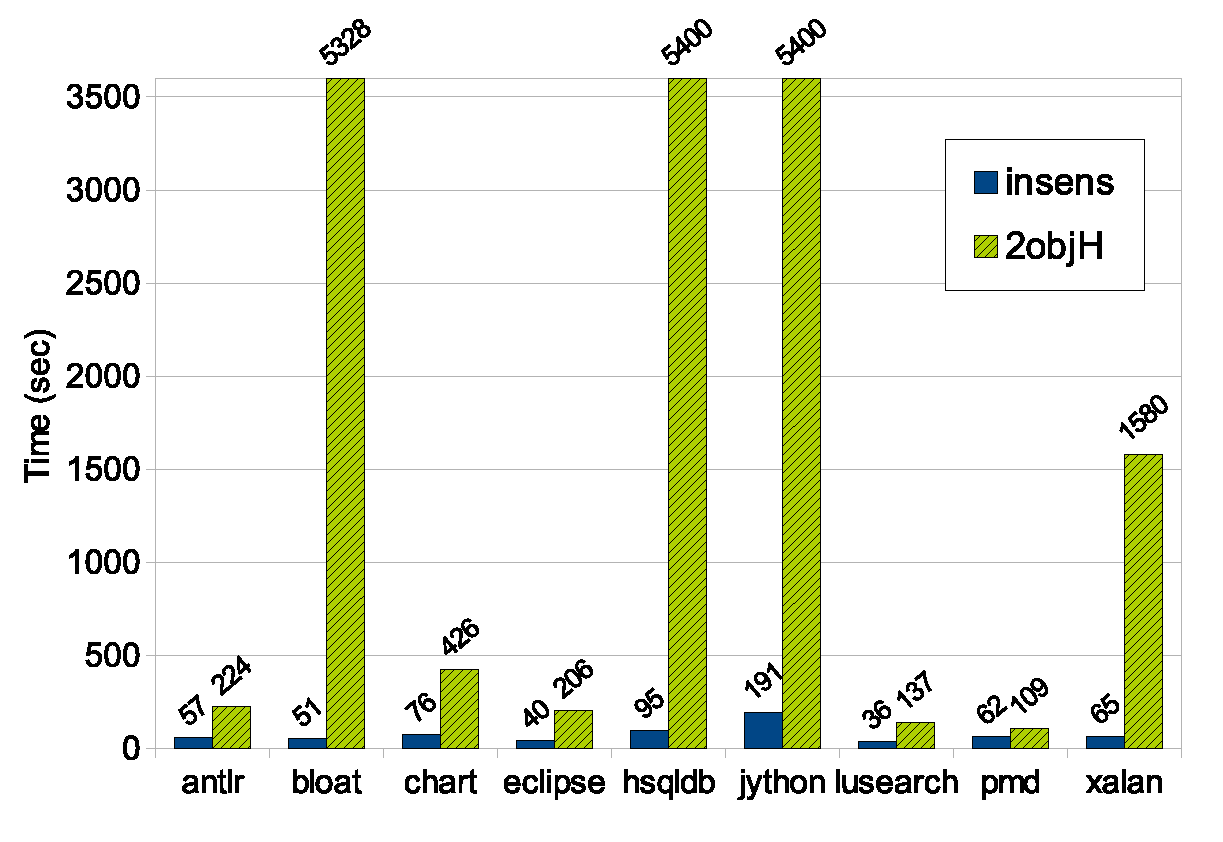
\includegraphics[scale=0.42]{assets/introspective/intro-chart.pdf}
\end{center}
\vspace{-0.6cm}
\caption{Comparison of running times of context-insensitive analysis vs. 2-object-sensitive with context-sensitive heap. The y-axis is truncated to 1hr for readability.}
\label{fig:introspect:intro}
\end{figure}

Faced with this unpredictability of context-sensitivity, a common reaction is to avoid it, favoring context-insensitive analyses, and, consequently, missing significant precision benefits for well-behaved programs. Even worse, for some applications, eschewing expensive context-sensitivity is not an option---a context-insensitive analysis is just not good enough and even an often inexpensive context-sensitive analysis (e.g., 2-type-sensitive with a context-sensitive heap) fails to yield good precision. Reports from industry~\cite{misc:Cifuentes} and academic researchers~\cite{misc:Chong} alike reiterate that precise context-sensitivity is essential for information-flow analysis, taint analysis, and other security analyses.

We can ask ourselves, why does this scalability barrier arise? The core problem is that, for some objects or methods, the points-to information is imprecise enough that more context does not help, while incurring a heavy overhead \cite{popl:2011:Smaragdakis}. Consider a method argument that was found to point to $n$ objects by a less precise analysis. Further analyzing the method in $c$ different contexts (or, equivalently, increasing context depth by 1) will ideally yield $n/c$ points-to facts per context, perfectly splitting the previous $n$-object points-to set, thus yielding both precision and scalability. In the worst case, however, increasing the context depth will result in $c$ copies of $n$ points-to facts each: the extra context depth will not have yielded more precision, but will have multiplied the space and time costs. When this occurs, the analysis cost explodes for greater context depths.

The focus of this chapter is on the detection and prevention of pathological behavior in context-sensitive analyses, with minimal intervention. In this way, we achieve many of the precision benefits of context-sensitivity without sacrificing scalability. It does not seem possible to know in advance (e.g., by identifying syntactic features of the program) which program elements may be responsible for pathological behavior. Nevertheless, we argue that it is possible to identify such elements with a scalable context-insensitive analysis. We introduce the concept of \emph{introspective context-sensitivity}: during a first, context-insensitive, analysis pass, the analysis observes symptoms indicating that the cost may get out of hand for deeper context. This detects exactly the pathology identified above. In its simplest form, the analysis will ask ``which program sites currently have points-to information that may grow too large for an extra level of context?'' Using a configurable second pass\footnote{In theory, this pattern could be repeated for more passes.}, such sites will be re-analyzed with shallow context, even though the rest of the program will be re-analyzed with a deeper context.

In intuitive terms, introspective context-sensitivity performs a cost-benefit calculation, with an emphasis on the potential cost of increasing context depth, since cost can be estimated more reliably. Fairly simple---yet not always obvious---heuristics can estimate this cost well. 

As a general pattern, this approach is familiar. Even in the context of points-to analysis, the pattern of performing a coarse-grained analysis and using it to tune a finer-grained one has been explored before, as in earlier \emph{refinement-based}~\cite{pldi:2006:Sridharan} or \emph{pruning}~\cite{pldi:2011:Liang} techniques. Nevertheless, such past approaches differ from our approach in terms of both external applicability and impact: they fundamentally apply to demand-driven (as opposed to all-points on the entire program) analyses and they either do not target context depth or only apply to specific kinds of context---related work in Section~\ref{sec:related:introspective} includes a detailed discussion.

The net outcome of our work is not a ``first line of defense'' analysis, but an ``if all else fails'' analysis. Users are still better advised to first use traditional context-sensitive algorithms, in the hope that these will scale well and provide good precision. When this fails, however, we show that we can provide a highly reliable knob for filtering out worst-case performance at a small cost in precision. Our experiments demonstrate that the user can ``dial-in'' scalability, to the exact level required. For instance, as seen in Figure~\ref{fig:introspect:intro}, a precise 2objH analysis fails to run in under 90mins on a 24GB machine for 3 of our experimental subjects. However, we can get an introspective context-sensitive analysis to scale to all benchmarks in under 12mins, while still gaining significant precision over a context-insensitive analysis. Yet another introspective analysis scales to all but one benchmark in under 20mins, while sacrificing a fraction of precision (keeping about 2/3 of the precision gains of a full 2objH analysis). For call-site sensitive analyses, the gains are even more pronounced, with several benchmarks exhibiting at least 300\% speedups, without sacrificing nearly any precision.

Overall, this chapter describes the following contributions:

\begin{itemize}
\item We offer an approach to refining a context-sensitive analysis while avoiding its worst-case cost. The approach relies on first running a context-insensitive analysis and using its results to inform the application of context-sensitivity. Much of the challenge concerns the question of \emph{how} to use this information, i.e.,  what heuristics yield good behavior.

\item We encode the approach in a simple form, by incremental modifications of a general declarative analysis pattern. Therefore, our approach works on virtually any algorithm expressed in this manner. Our implementation is on the \doop{} framework and already applies to the over 30 analysis algorithms that the framework has to offer.

\item We show experimentally the benefit of introspective context-sensitivity. We quantify the precision loss and scalability gains for different parameter settings and show that there is a dial that users can tune, to select points in this spectrum. Even our high-precision settings are effective in eliminating behavior outliers, showing that introspective context-sensitivity has core value: previously hopeless analyses suddenly become feasible, for little precision loss. We believe that the result is to give confidence that context-sensitive analyses can be used in virtually any setting and not just in the nebulous ``when they work well'' case.
\end{itemize}

\section{Formulation of Introspective Context-Sensitivity}
\label{sec:introspect:model}

We demonstrate introspective context-sensitivity via incremental changes to the existing model for context-sensitive, flow-insensitive points-to analysis algorithms presented in Section~\ref{sec:back:model}. As previously mentioned, the logical formalism of this model is very close to the core components of our actual analysis implementation.

\paragraphhead{Input relations.}
Two additional input relations are added to those presented in Figure~\ref{fig:back:input} and are used exclusively for the purposes of introspective context-sensitivity. \relname{SiteToRefine} and \relname{ObjectToRefine} encode the program points (invocation site/method combinations, and allocation sites) that will employ a different context abstraction from the rest.

\begin{figure}[hb]
\begin{datalog}
\rel{SiteToRefine}{invo: I, meth: M} \\ 
\rel{ObjectToRefine}{heap: H}
\end{datalog}
\caption[]{Additional input Datalog relations expanding those of Figure~\ref{fig:back:input}.}
\label{fig:introspect:input}
\end{figure}

\paragraphhead{Computed (output) relations.}
No additional output relations need to be added to those of Figure~\ref{fig:back:output}.

\paragraphhead{Constructors for context-sensitivity.}
As previously mentioned, the base rules of any analysis are not concerned with what kind of context-sensitivity is used. The context flavor and depth aspects are completely hidden mainly behind constructor functions \consname{Record} and \consname{Merge}. These functions are sufficient for modeling a very large variety of context-sensitive analyses. In addition to those two, introspective context-sensitivity adds two more constructor functions to act as counterparts---\consname{RecordRefined} and \consname{MergeRefined}. They are directly analogous to \consname{Record} and \consname{Merge} but just apply to different program points. These constructors are the machinery for introspective context-sensitivity: they vary the context-sensitivity of the analysis for a subset of the heap objects and methods.

\begin{figure}[htp]
\begin{datalog}
\cons{RecordRefined}{heap: H, ctx: C}{newHCtx: HC} \\
\cons{MergeRefined}{heap: H, hctx: HC, invo: I, ctx: C}{newCtx: C}
\end{datalog}
\caption[]{Additional constructors of contexts that filter which objects and which call-sites/target methods should have a different (i.e., more precise) context in introspective context-sensitivity.}
\label{fig:introspect:output}
\end{figure}

\paragraphhead{Analysis logic.}
The rules for introspective context-sensitivity supplement the existing logic presented in Section~\ref{sec:back:model}. Out of the core nine rules, only two need to be enhanced with duplicate versions, as shown in Figure~\ref{fig:introspect:rules}. Each rule pair offers a version for the default handling of context and another for the more precise handling. (In the full implementation, there are some two-dozen rules that construct new contexts, instead of the two in the model, and all are duplicated accordingly.)

The first pair considers the handling of object allocation, with the first rule applying when the allocation is to be treated with no additional precision, whereas the second applies a more refined context---whether the \relname{ObjectToRefine} holds or not for the current allocation site. The different handling of context is controlled via the \consname{Record} and \consname{RecordRefined} functions, respectively.

The second pair is somewhat more involved but still follows the same reasoning, applied to method invocations. The filtering is controlled via the \relname{SiteToRefine} relation and the different handling of (calling) context is done via the \consname{Merge} and \consname{MergeRefined} functions.

Therefore, we can effect any change we want to the context-sensitivity of an analysis, on a per-object/per-call-site basis, by supplying the right input relations \relname{ObjectToRefine} or \relname{SiteToRefine} and setting the appropriate constructors, \consname{RecordRefined} and \consname{MergeRefined} to implement a different flavor/depth of context-sensitivity. We discuss such options next.

\begin{figure}[h!tp]
\begin{datalog}
\cons{Record}{heap, ctx}{?hctx}, \\
\commrel{VarPointsTo}{var, ctx, heap, ?hctx} \dlIf{} \\
    \commrel{Reachable}{meth, ctx}, \commrel{Alloc}{var, heap, meth}, \\
    ! \rel{ObjectToRefine}{heap}. \\
\\
\comm{// Duplicate rule, for introspective context-sensitivity} \\
\cons{RecordRefined}{heap, ctx}{?hctx}, \\
\commrel{VarPointsTo}{var, ctx, heap, ?hctx} \dlIf{} \\
    \commrel{Reachable}{meth, ctx}, \commrel{Alloc}{var, heap, meth}, \\
    \rel{ObjectToRefine}{heap}. \\
%
\noindent\rule{\textwidth}{0.5pt}\\
%
\cons{Merge}{heap, hctx, invo, callerCtx}{?calleeCtx}, \\
\commrel{Reachable}{toMeth, ?calleeCtx}, \\
\commrel{VarPointsTo}{this, ?calleeCtx, heap, hctx}, \\
\commrel{CallGraphEdge}{invo, callerCtx, toMeth, ?calleeCtx} \dlIf{} \\
    \commrel{VCall}{base, sig, invo, inMeth}, \\
    \commrel{Reachable}{inMeth, callerCtx}, \\
    \commrel{VarPointsTo}{base, callerCtx, heap, hctx},\\
    \commrel{HeapType}{heap, heapT}, \\
    \commrel{Lookup}{heapT, sig, toMeth},\\
    \commrel{ThisVar}{toMeth, this}, \\
    ! \rel{SiteToRefine}{invo, toMeth}. \\
\\
\comm{// Duplicate rule, for introspective context-sensitivity} \\
\cons{MergeRefined}{heap, hctx, invo, callerCtx}{?calleeCtx}, \\
\commrel{Reachable}{toMeth, ?calleeCtx}, \\
\commrel{VarPointsTo}{this, ?calleeCtx, heap, hctx}, \\
\commrel{CallGraphEdge}{invo, callerCtx, toMeth, ?calleeCtx} \dlIf{} \\
    \commrel{VCall}{base, sig, invo, inMeth}, \\
    \commrel{Reachable}{inMeth, callerCtx}, \\
    \commrel{VarPointsTo}{base, callerCtx, heap, hctx},\\
    \commrel{HeapType}{heap, heapT}, \\
    \commrel{Lookup}{heapT, sig, toMeth},\\
    \commrel{ThisVar}{toMeth, this}, \\
    \rel{SiteToRefine}{invo, toMeth}.
\end{datalog}
\caption[]{Datalog rules for different handling of context creation on a per-object/per-call-site basis.}
\label{fig:introspect:rules}
\end{figure}


\section{How To Selectively Refine}
\label{sec:introspect:heuristics}

The model of the previous section allows to easily configure context-sensitivity in a large variety of ways. For instance, some methods (or some call-sites) can be analyzed with object-sensitivity while others are analyzed with call-site sensitivity, of any depth. One aspect to determine, therefore, is the two analyses that will be used in different program points.

Another question is how to populate the \relname{ObjectToRefine} and \relname{SiteToRefine} input relations. One could attempt to do so by mere syntactic inspection of the program. For example, methods containing cast statements can be analyzed with a higher context depth. In our work, we have failed to identify such syntactic heuristics that would yield benefit.

Instead, our introspective context-sensitivity consists of running the analysis \emph{twice}. The first time, \relname{ObjectToRefine} and \relname{SiteToRefine} are \emph{empty} and the \consname{Merge}/\consname{Record} context constructors are set so that an inexpensive but scalable analysis is performed. In our experimental setting, these constuctor functions return a unique constant value, \args{$\star$}, resulting in a context-insensitive analysis:

\begin{quote}
\cons{Record}{heap,ctx}{$\star$}\\
\cons{Merge}{heap, hctx, invo, ctx}{$\star$} \\
\end{quote}

The \consname{MergeRefined} and \consname{RecordRefined} constructors are set to implement an expensive context-sensitive analysis, following the techniques of Chapter~\ref{chapter:hybrid}. Yet, these constructors are not relevant in the first analysis run, since the rules employing them are predicated on having elements in \relname{SiteToRefine} and \relname{ObjectToRefine}, respectively.

Subsequently, we use the results of the context-insensitive analysis to compute which program elements to refine (i.e., populate the \relname{SiteToRefine} and \relname{ObjectToRefine} relations), and run the analysis a second time. The result is that a subset of the program elements are analyzed context-sensitively, while the rest are analyzed context-insensitively even during the second analysis run. In practical terms, the former set is larger than the latter: we focus on identifying a relatively small number of program elements that may disproportionately affect analysis costs and to analyze them context-insensitively, while the majority of program elements are analyzed context-sensitively.

Therefore, the main challenge is to identify a program client analysis (over the results of a context-insensitive points-to analysis) to predict which program elements should not be refined. Our criterion is based on cost rather than expected benefit, since the latter is very hard to estimate in an all-points (as opposed to demand-driven) program analysis. There are several cost metrics that we can mix-and-match to create introspective analysis heuristics:

\begin{enumerate}
\item \label{metric-arginflow} Compute at every invocation site the cumulative size of all points-to sets of actual arguments to the method call. (This is the argument \emph{in-flow} of the method call.)

\item \label{metric-methvpt} Compute for every method the cumulative (or maximum, for a variant of the metric) size of points-to sets over all local variables. (This is the method's \emph{total points-to volume} or \emph{max var-points-to}.)

\item \label{metric-maxfield} Compute for each object (i.e., allocation site) the maximum (or total, for a variant of the metric) field points-to set over all of its fields (This is the object's \emph{max field points-to}, or \emph{total field points-to}.)

\item \label{metric-methodmaxfield} Compute for every method the maximum max field-points-to (metric~\ref{metric-maxfield}) among objects pointed to by the method's local variables. (This is the method's \emph{max var-field points-to}.)

\item \label{metric-pointedby} Compute for each object (i.e., allocation site) the number of local variables pointing to it. (This is the object's \emph{pointed-by} metric.)
\end{enumerate}

As can be seen, these metrics can vary in sophistication but all of them attempt to estimate the cost that will be incurred if the same method or allocation site were to be analyzed context-sensitively. Indeed, our emphasis is not on the sophistication of the metrics or on their fine-tuning. Instead, it is on their simplicity and ease of composition so that one can create parameterizable analyses: a knob for adjusting the precision/scalability tradeoff. For example, we propose two heuristic combinations of these metrics:

\begin{quote}
\paragraphhead{Heuristic-A.}
% tempH heuristic in the initial source code
Refine all allocation sites except those with a \emph{pointed-by} (Metric~\#\ref{metric-pointedby}) higher than a constant $K$.  Refine all method call-sites except those with either an \emph{in-flow} (Metric~\#\ref{metric-arginflow}) higher than a constant $L$ or a \emph{max var-field points-to} (Metric~\#\ref{metric-methodmaxfield}) higher than a constant $M$.
\end{quote}

\begin{quote}
\paragraphhead{Heuristic-B.}
% tempO heuristic in the initial source code
Refine all method call-sites except those that invoke methods with a \emph{total points-to volume} (Metric~\#\ref{metric-methvpt}) above a constant $P$. Refine all object allocations except those for which the product of \emph{total field points-to} and \emph{pointed-by} (Metrics~\#\ref{metric-maxfield} and \#\ref{metric-pointedby}) exceeds a constant $Q$. The product of these two metrics can be seen as an object's total potential for weighing down the analysis.
\end{quote}

These heuristics are themselves tunable, by adjusting the constant parameters. In the rest of the chapter, when we refer to \emph{Heuristic-A} in measurements, the values of $K$, $L$, $M$ will be 100, 100, and 200, respectively; when we refer to \emph{Heuristic-B}, the values of $P$ and $Q$ will both be 10000. The point of picking clear-cut reference numbers is to argue that the value of the technique does not come from excessive tuning but from the underlying power of the introspective analysis idea---even relatively large variations of these numbers make scarcely any difference in the total picture of results over multiple programs.

\paragraph*{Intuition.} 
The main insight behind our Heuristic-Approach is that there are many program elements whose analysis cost is vastly disproportionate to their importance. If such elements are analyzed less precisely, the analysis will avoid significant burden without incurring large precision losses. The above two heuristics try to estimate ``disproportionate cost'' but have no way of estimating the ``importance'' of a program element. It would be an interesting direction for future work to estimate this importance, i.e., to define metrics that capture the extent of the impact of a program element's precision on all other program elements.

Furthermore, a program element with very large cost, in terms of associated points-to facts, may be hopeless for good enough precision anyway. On the other hand, the above intuition could potentially unfold the other way: it is possible that context-sensitivity can productively distinguish seemingly-imprecise program elements (e.g., methods with large cumulative points-to sets, but also many callers) and maintain precision.

\paragraph*{Implementation.}
The above metrics and heuristics can be easily implemented as short analyses over the result of a context-insensitive points-to analysis. For instance, the implementation of the \emph{in-flow} metric (\#\ref{metric-arginflow}) is the following Datalog rules, which define an intermediate predicate and aggregate over it. (``\args{\_}'' is a nameless variable denoting any value, and ``\texttt{\{...\}}'' denotes an aggregate operation over the relations inside the curly brackets---in our case a total count of matching tuples.)

\begin{figure}[h]
\begin{datalog}
\rel{HeapsPerInvocationPerArg}{invo, arg, heap} \dlIf{} \\
    \rel{CallGraphEdge}{invo, \_, \_, \_},\\
    \rel{ActualArg}{invo, \_, arg},\\
    \rel{VarPointsTo}{arg, \_, heap, \_}.\\
\\
\rel{InFlow}{invo, ?result} \dlIf{} \\
    \aggregate{COUNT}{\rel{HeapsPerInvocationPerArg}{invo, \_, \_}}{?result}.
\end{datalog}
\end{figure}




\section{Evaluation}

Our evaluation setting uses the \todo{} LogicBlox Datalog engine, v.3.9.0, on a Xeon E5530 2.4GHz machine with only one thread running at a time and 24GB of RAM. We analyze the DaCapo benchmark programs (v.2006-10-MR2) with Open JDK 1.6.0\_24. We run all benchmarks with default \doop{} settings, including full reflection support. We selected a priori 6 of the Dacapo benchmarks as our experimental subjects: these are the programs that exhibit scalability problems based on past literature (e.g., Chapter~\ref{chapter:hybrid}). Other benchmarks typically run in half the time of the fastest benchmark of our set for deep context-sensitive analyses. Since our technique is explicitly not a ``first line of defense'', benchmarks that are already certain to scale are out of scope.

\begin{figure*}[h!tp]
\begin{center}
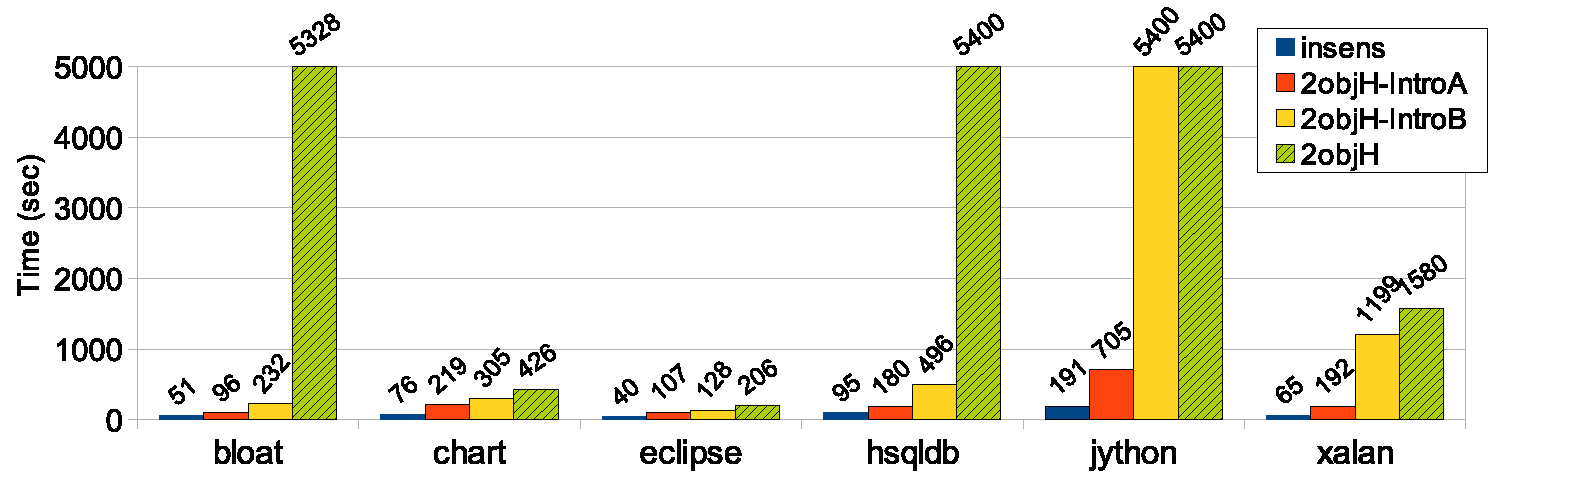
\includegraphics[scale=0.54]{assets/introspective/2objHtime.pdf} \\
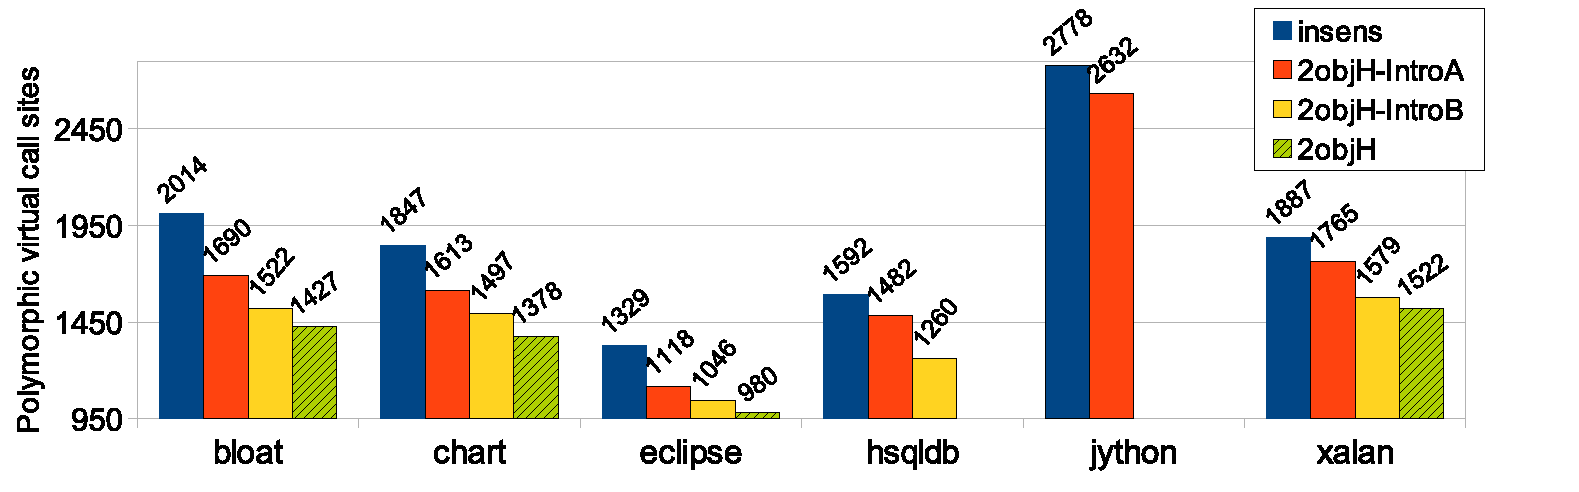
\includegraphics[scale=0.54]{assets/introspective/2objHvcalls.pdf} \\
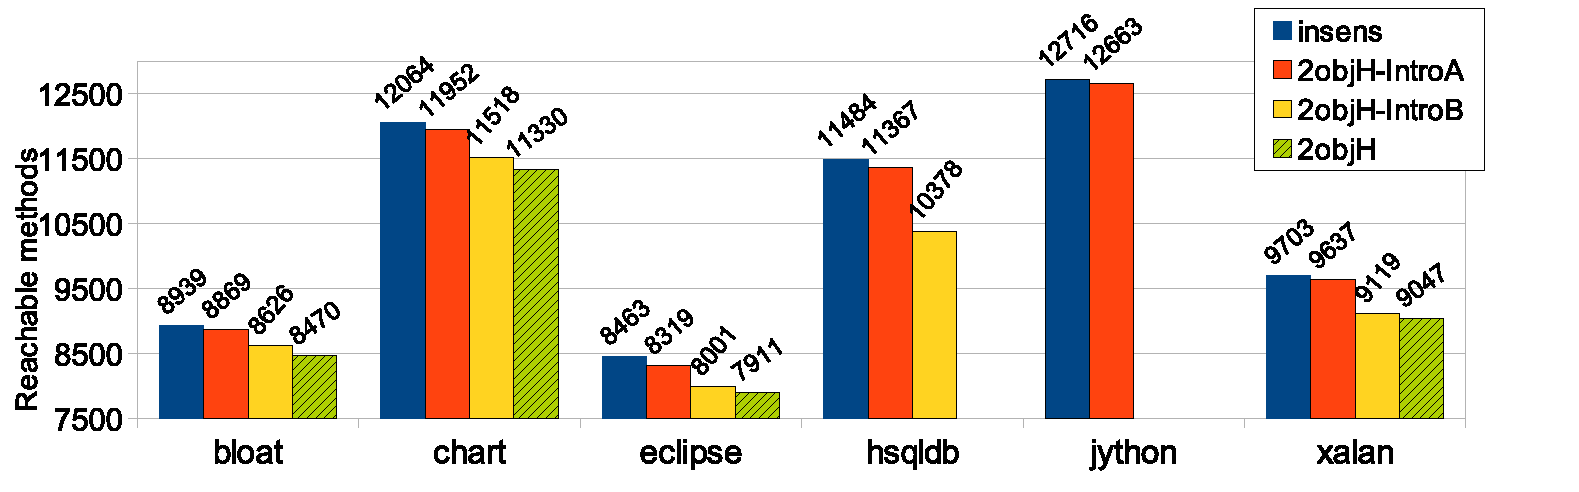
\includegraphics[scale=0.54]{assets/introspective/2objHmeths.pdf} \\
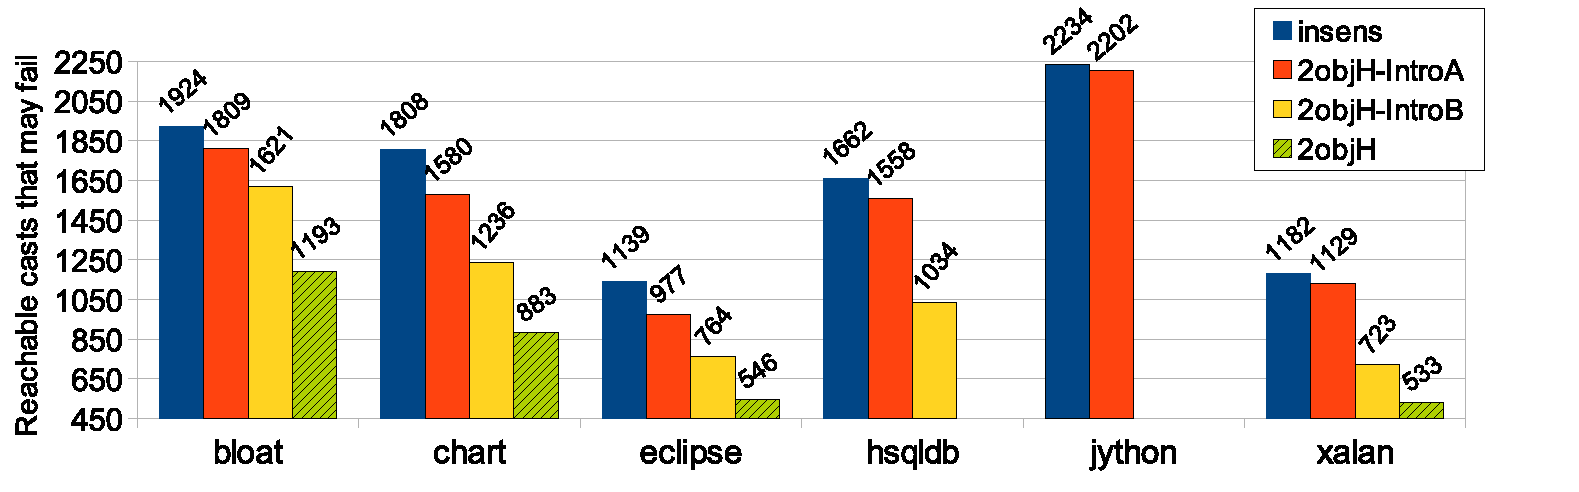
\includegraphics[scale=0.54]{assets/introspective/2objHcasts.pdf}
\end{center}
\caption{Performance and precision (3 separate metrics: calls that cannot be devirtualized, reachable methods, casts that cannot be eliminated) for introspective context-sensitive variants of a \textbf{2objH} analysis, compared with baselines (2objH and insensitive).}
\label{fig:introspect:2objH-chart}
\end{figure*}


\begin{figure*}[h!tp]
\begin{center}
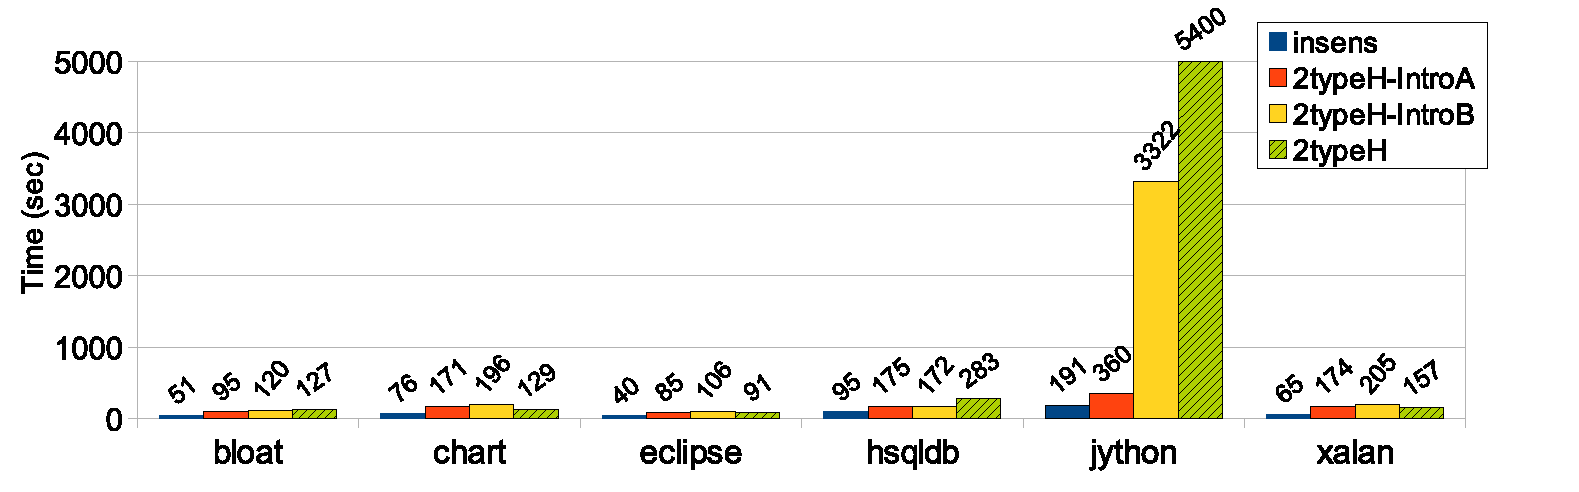
\includegraphics[scale=0.54]{assets/introspective/2typeHtime.pdf} \\
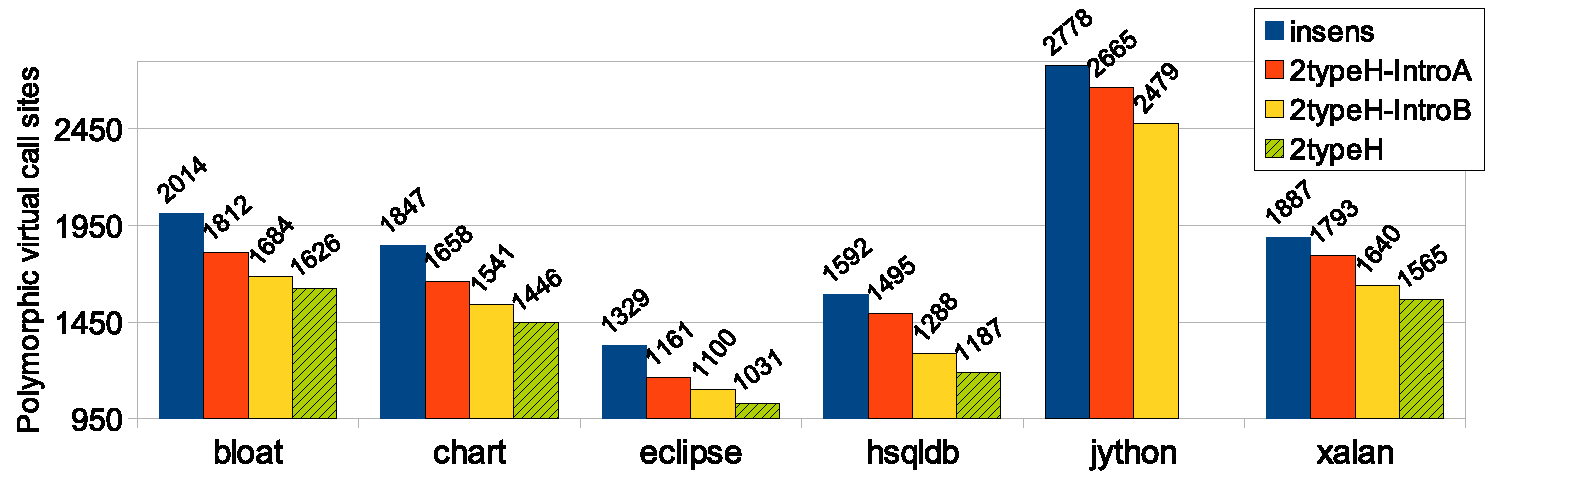
\includegraphics[scale=0.54]{assets/introspective/2typeHvcalls.pdf} \\
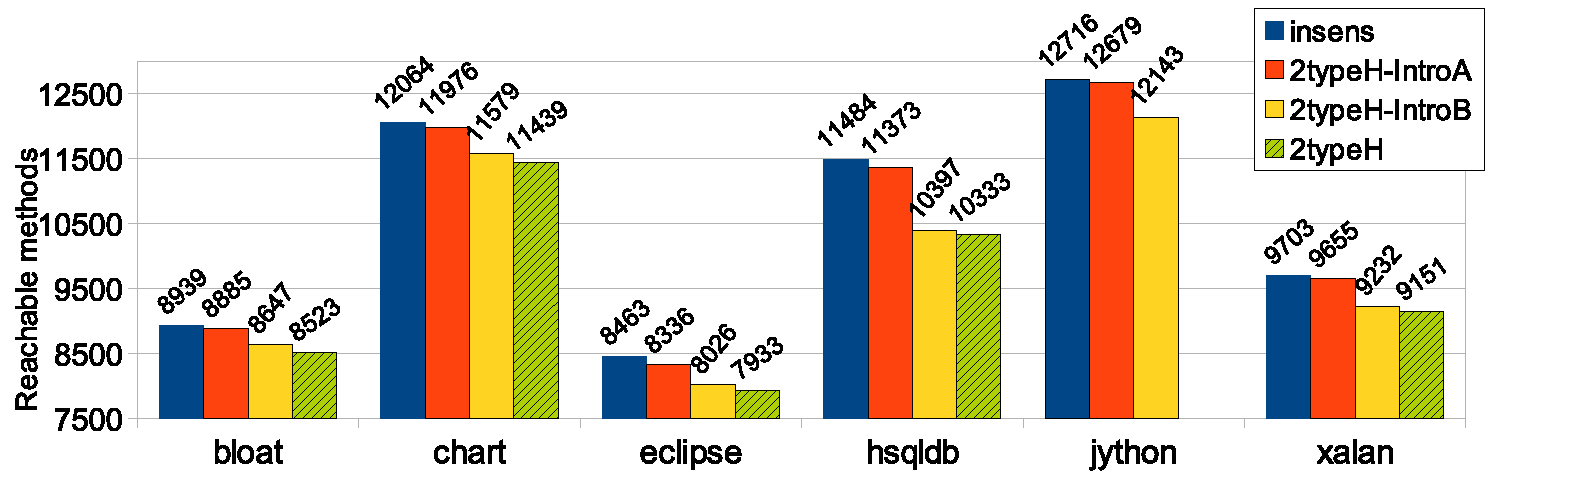
\includegraphics[scale=0.54]{assets/introspective/2typeHmeths.pdf} \\
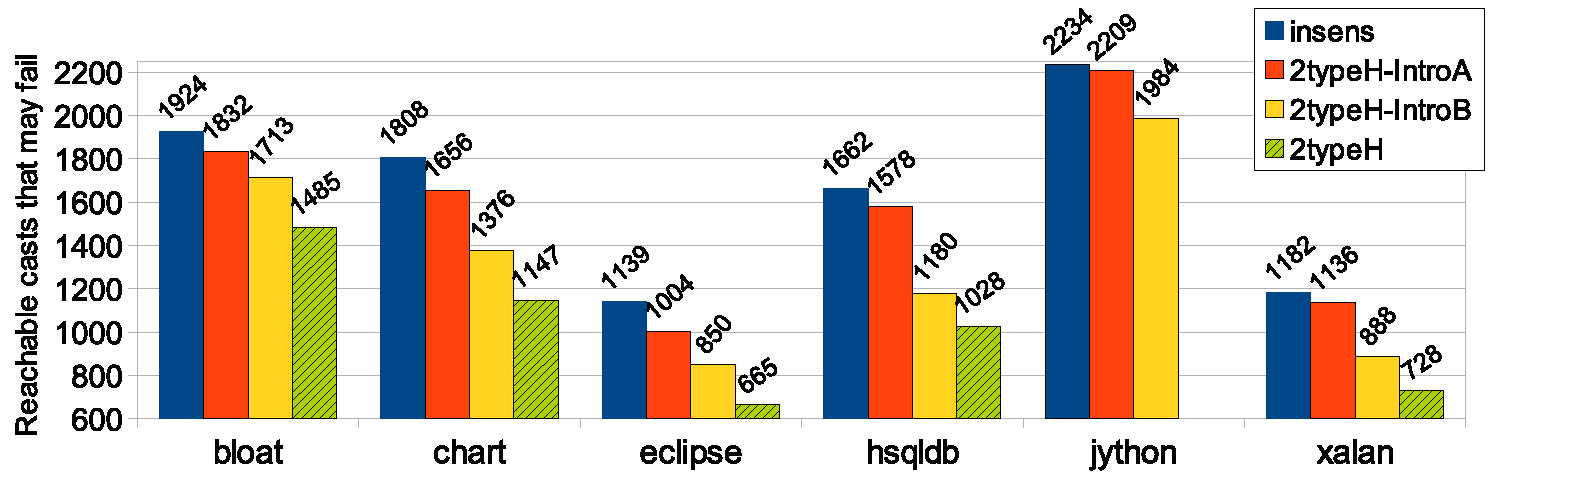
\includegraphics[scale=0.54]{assets/introspective/2typeHcasts.pdf}
\end{center}
\caption{Performance and precision (3 separate metrics: calls that cannot be devirtualized, reachable methods, casts that cannot be eliminated) for introspective context-sensitive variants of a \textbf{2typeH} analysis, compared with baselines (2typeH and insensitive).}
\label{fig:introspect:2typeH-chart}
\end{figure*}


\begin{figure*}[t!bp]
\begin{center}
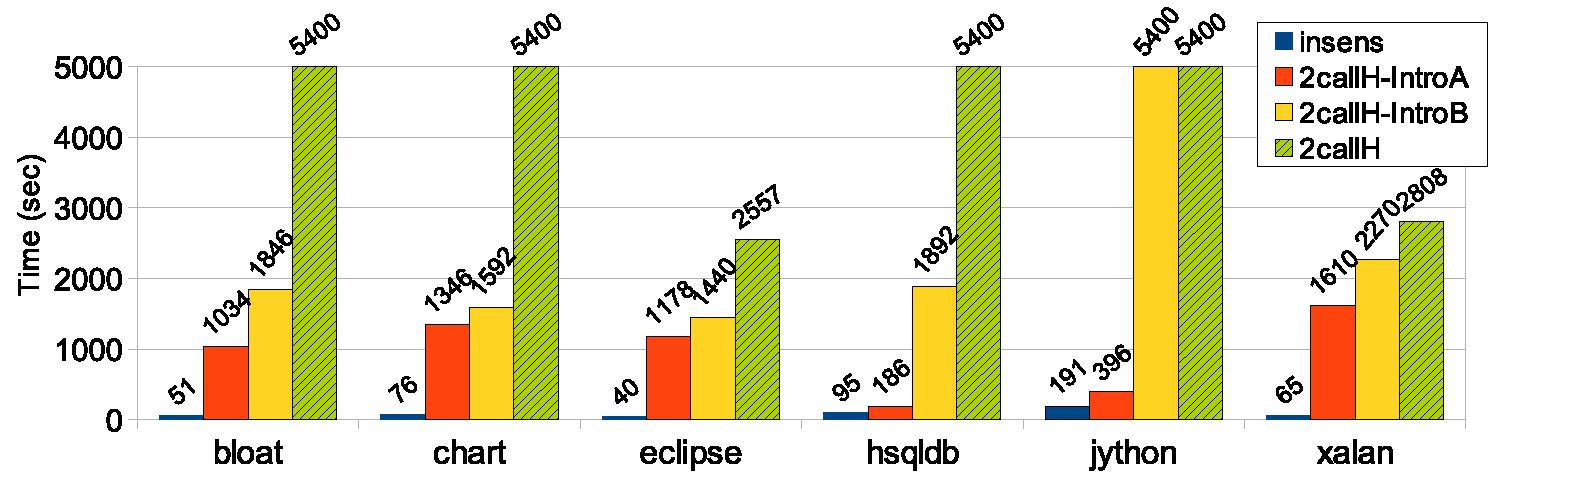
\includegraphics[scale=0.54]{assets/introspective/2callHtime.pdf} \\
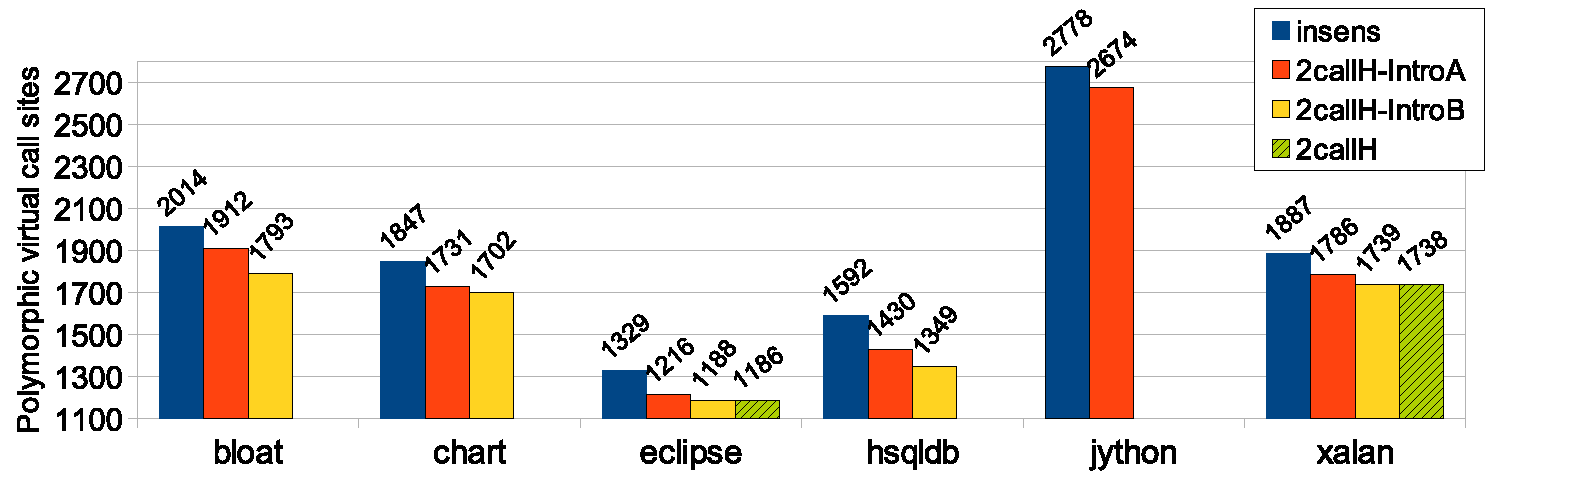
\includegraphics[scale=0.54]{assets/introspective/2callHvcalls.pdf} \\
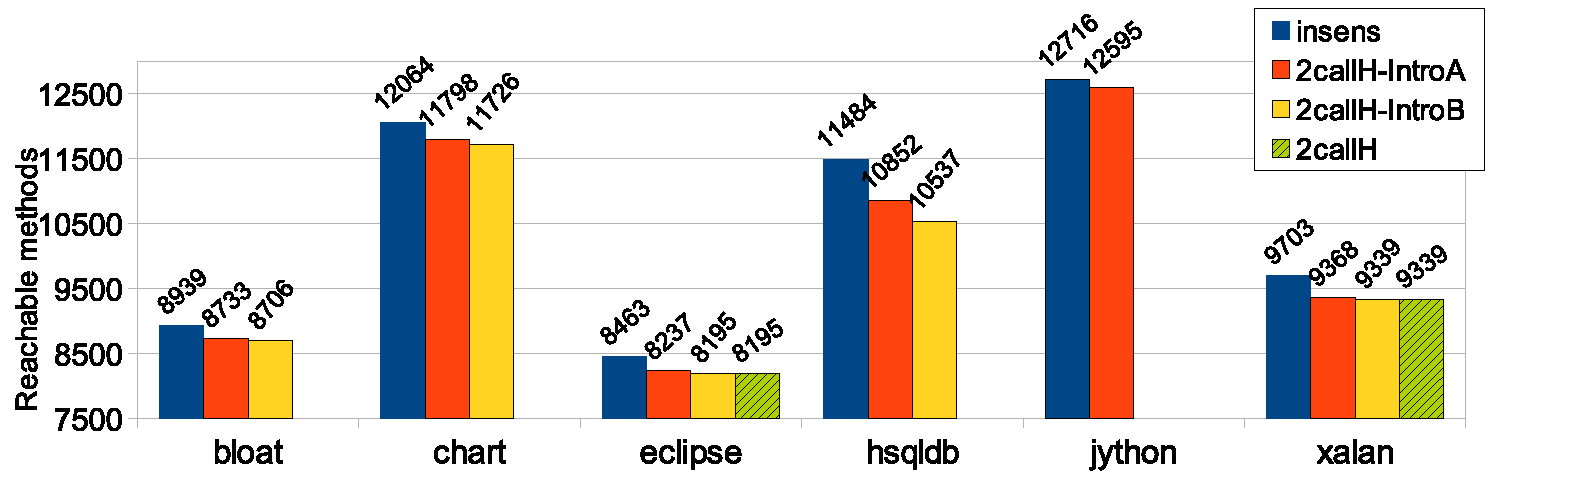
\includegraphics[scale=0.54]{assets/introspective/2callHmeths.pdf} \\
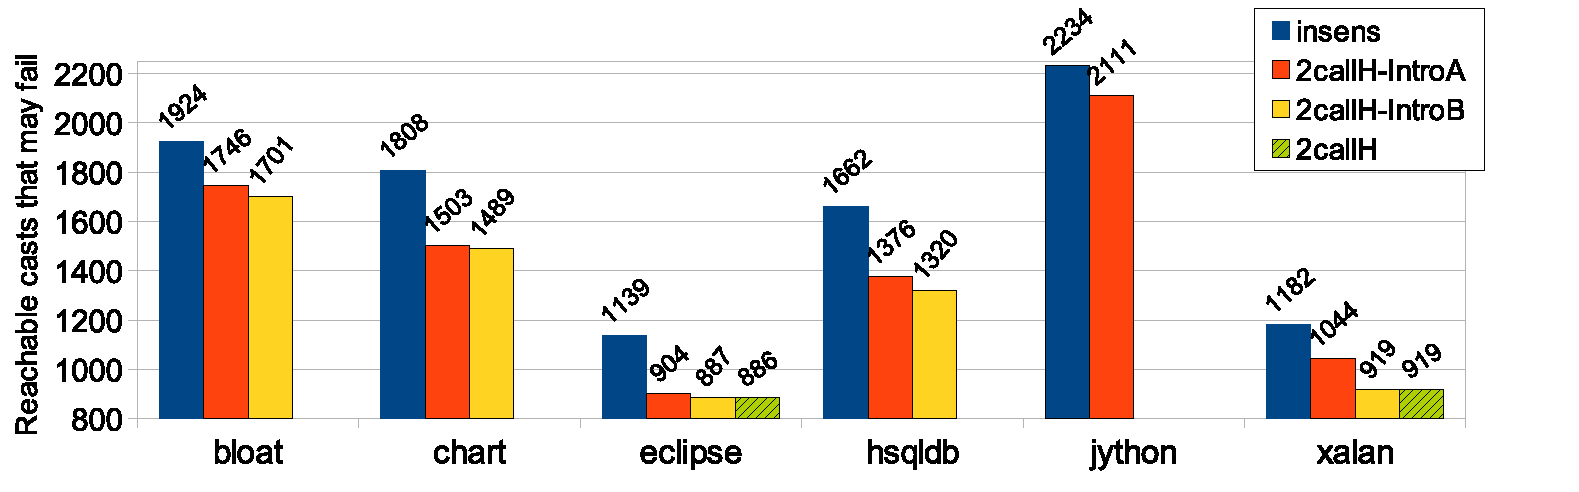
\includegraphics[scale=0.54]{assets/introspective/2callHcasts.pdf}
\end{center}
\caption{Performance and precision (3 separate metrics: calls that cannot be devirtualized, reachable methods, casts that cannot be eliminated) for introspective context-sensitive variants of a \textbf{2callH} analysis, compared with baselines (2callH and insensitive).}
\label{fig:introspect:2callH-chart}
\end{figure*}


The results of our experiments are shown in Figures~\ref{fig:introspect:2objH-chart}, \ref{fig:introspect:2typeH-chart}, and \ref{fig:introspect:2callH-chart}. We evaluate two variants of introspective context-sensitivity corresponding to \emph{Heuristic-A} and \emph{Heuristic-B} from Section~\ref{sec:introspect:heuristics}. We test the three main flavors of context-sensitivity: object-sensitivity \cite{issta:2002:Milanova,article:2005:Milanova}, call-site sensitivity \cite{col:1981:Sharir,thesis:Shivers}, and type-sensitivity~\cite{popl:2011:Smaragdakis}. The three flavors have very different profiles of practical use and scalability, as detailed next.


\subsection{Object-sensitivity}
Deep-context object-sensitive analyses are the most precise in practice, but do not always scale well. Starting from a 2-object-sensitive analysis with a 1-context-sensitive heap (2objH), we define our two introspective versions (2objH-IntroA and 2objH-IntroB for Heuristic-A and Heuristic-B, respectively). Figure~\ref{fig:introspect:2objH-chart} plots first the execution time and then three precision metrics for all analyses. In all cases \emph{lower is better}. There is no real ``metric'' for precision, since each client may have unique needs, but our three metrics together should yield a reasonable projection of precision. Note that since there is no ``ground truth'' for the ideal value of precision metrics, their chart scales are arbitrary (and differences are not as visually pronounced as could be because of plotting multiple benchmarks on a single chart) but the insensitive/2objH analyses serve as upper/lower reference markers in practice. We use a 90min timeout. The jython and hsqldb benchmarks did not terminate for 2objH, and jython did not terminate for 2objH-IntroB either. We indicate non-termination with full bars in the top (time) chart and the absence of bars in the bottom three (precision) charts.

As can be seen in Figure~\ref{fig:introspect:2objH-chart}, the two introspective variants scale much better than the full 2objH analysis. Indeed, IntroA scales to all benchmarks, while showing significant precision gains over an insensitive analysis. IntroB is even more precise: it covers \emph{more than two-thirds} of the precision advantage of 2objH over an insensitive analysis for most benchmarks and precision metrics, while scaling significantly better.


\subsection{Type-sensitivity}
Type-sensitivity is designed with the explicit purpose of providing more scalability than object-sensitivity but in a very different manner: instead of avoiding high context depths, type-sensitivity makes each context element coarser. Thus it is doubly interesting to see if introspection can add benefit to type-sensitive analyses. Type-sensitivity is not immune to the pathologies of object-sensitivity: for instance, in our benchmark set it does not scale to jython. 

Figure~\ref{fig:introspect:2typeH-chart} shows our results, plotting variants of a 2-type-sensitive analysis with a 1-context-sensitive heap (2typeH), and following the same conventions as earlier. (The insensitive baseline is inherited and not re-run.) As can be seen, the IntroB version scales to all programs while typically maintaining very good precision---often close to the full 2typeH. The IntroA version has the desirable feature of near-perfect scalability: its maximum runtime for \emph{any} benchmark is 360sec. At the same time it exhibits precision gains compared to a context-insensitive analysis, although these are noticeably lower than the precision gains of IntroB.


\subsection{Call-site sensitivity}
Call-site sensitivity is the traditional flavor of context-sensitivity---a virtual synonym for the term. In practice, call-site sensitivity is quite good for some analysis clients but almost never scalable at context depths greater than 1. 

As Figure~\ref{fig:introspect:2callH-chart} shows, introspective context-sensitivity performs remarkably well when applied to a 2-call-site-sensitive analysis with a 1-context-sensitive heap (2callH). The base 2callH analysis does not terminate for 4 out of 6 of our benchmarks, while introspective analyses terminate either for all (IntroA) or for nearly all (5 out of 6 for IntroB). Furthermore, IntroB seems to achieve the full precision of 2callH for the two benchmarks for which the latter yields results, and for all different metrics! Combined with the across-the-board scalability gains shown in the timing chart, this confirms the effectiveness of introspection for tuning out extreme analysis costs. IntroA is not far behind in precision, obtaining more than two-thirds of the precision gains of IntroB for most metrics and benchmarks.


\subsection{Discussion}
The above timings of introspective context-sensitivity do not include the cost of first running a context-insensitive analysis, and other timing overheads (relatively constant at about 100sec) related to computing the objects and sites to refine and re-running an analysis (our current implementation saves the first-run database and re-generates it from scratch \todo{}). We did not include these numbers in the timings in order to keep the presentation simpler but also because
\begin{inparaenum}[(a)]
\item our emphasis is on scalability and not on small-scale speed gains---we consider small differences in timings, e.g., in the chart and eclipse benchmarks of Figure~\ref{fig:introspect:2objH-chart}, to be negligible for our purposes; and
\item these constant overheads can be factored out---e.g., with minor engineering we could have incurred them only once per benchmark and not once per run of every introspective analysis variation.
\end{inparaenum}

Based on our experimental results, introspective context-sensitivity achieves its goal: it offers a knob for users to select points in the scalability/precision spectrum. The tradeoffs of cost and precision exhibited by Heuristic-A and Heuristic-B are illustrative. Not only do these heuristics yield different options (more precision vs. more scalability) but they are also very consistent in their tradeoff, throughout multiple benchmarks and analysis flavors.

Finally, note that we used identical introspection heuristics (Heuristic-A and Heuristic-B) with the same constants (see Section~\ref{sec:introspect:heuristics}) for all three context-sensitivity flavors and for all benchmarks. This suggests that there are significant opportunities for further tuning: different heuristics can be used, the constants can be optimized, the constants or the heuristics can be adapted per-benchmark or per-context flavor. However, the goal of our experiments is not to squeeze out a few percentage points of speedup but to show that the simple idea of introspective context-sensitivity can easily offer very useful tradeoffs in scalability and precision.


\section{Summary}

We introduced introspective context-sensitivity: an approach to making context-sensitive analyses scale. The approach consists of defining an analysis with two separate kinds of context. Each program element is analyzed with one kind, selected based on external input. Then, by first running an inexpensive context-insensitive analysis, we can identify program elements that should be treated with a more precise context and others that should be treated less precisely to avoid an explosion in complexity. Our technique applies to any kind of context abstraction and yields scalability \emph{\`{a} la carte}: the user can select a scalability profile and achieve it for a price in precision. As shown in our experiments, this price is not too steep. The precision loss of introspective context-sensitivity can be minuscule (as is for call-site-sensitive analyses), while the scalability gain is substantial.

We believe that introspective context-sensitivity is a big step forward in pointer analysis. It is not just an effective technique, but an effective technique that addresses the major current pain point in practical applications of points-to analyses.

\part{Achieving High-Confidence Results}
\chapter{Must-Alias Analysis: Logical Model}
\label{chapter:must-logic}
\epigraph{Logic, my dear Zoe, merely enables one to be wrong with authority.}{\textit{The 2nd Doctor} - Doctor Who}

As previously mention at the beginning of Chapter~\ref{chapter:intro}, alias analysis is closely related to pointer analysis with the difference being that the main goal of alias analysis is finding aliasing among program expressions whereas the main goal of pointer analysis is to reason about the objects that program expressions may point to. In both case, one can be employed to support the reasoning of the other.

The vast majority of pointer analysis techniques that have appeared in the recent research literature (e.g., \cite{pldi:1999:Yong,pldi:2003:Berndl,cc:2013:Kastrinis,pldi:2007:Hardekopf,article:2005:Milanova,pldi:2004:Whaley,pldi:2006:Sridharan}) are \emph{may}-analyses. That is, the techniques attempt to \emph{over}-approximate an unattainable, fully precise result (recall Section~\ref{sec:back:may-must}). All possible aliasing expressions are guaranteed to be included in the outcome of a may-alias analysis. All possible abstract objects that may be referenced by a variable are included in the variable's may-point-to set. However, spurious inferences---which will never occur in program execution---may also be included in the analysis output.

In contrast, an \emph{under}-approximate, \emph{must}-analysis (or \emph{definite}-analysis) is often desirable. A must-analysis computes aliasing or points-to relationships that are guaranteed to always hold during program execution, at the cost of missing some inferences. In practice, a must-alias analysis is more probable than a must-points-to analysis. Aliasing relationships are more generally provable from local inspection of the program text, whereas points-to facts are harder to establish in a conservative must- fashion. The difficulty is dual: First, the allocation sites of objects are often far from their use sites, making the establishment of must-points-to relationships unlikely. Second, must-points-to reasoning requires careful modeling of abstract vs. concrete objects. For instance, for techniques such as \emph{strong updates} (i.e., replacing the value of an object field at a store instruction) it is not sufficient to know the abstract object that the base expression must-points-to, since the abstract object may conflate many concrete objects during program execution (e.g., in a loop), and only one of them will have its field updated.

A must-alias analysis is typically flow-sensitive, i.e., it computes information per-program-point, respecting the control-flow of the program (recall Section~\ref{sec:back:flowSensitivity}). It offers several applications:

\begin{itemize}
\item It is useful for optimizations---e.g., constant folding, common subexpression elimination, and register allocation;

\item It can increase the precision of bug detectors (that traditionally have a high false-warnings rate): Nikoli\'{c} and Spoto~\cite{ictac:2012:Nikolic} report that a must-alias analysis significantly increases the precision of both a null-reference detector (46\% fewer warnings) and a non-termination detector (11\% fewer warnings). Earlier work has reported similar benefits~\cite{isola:2008:Ma};

\item It can be used as an internal component as part of a more complex analysis. For instance, must-alias results may enable an analysis to perform ``strong updates'' at instructions that modify the heap. Earlier work has used must-alias analysis to similar benefit~\cite{pldi:1994:Emami,popl:1998:Jagannathan};

\item It can be invaluable for better program understanding; the results of a must-inference are guaranteed facts, of immediate value to the human programmer.
\end{itemize}

To illustrate must-alias reasoning, consider the code example in Figure~\ref{fig:must-logic:snippet}. Even at this size, inspecting the program requires human effort. The output consists of must-alias pairs: expressions that are guaranteed to point to the same object---denoted by ``$\sim$''. In this example, \code{a2.next} and \code{a1} form an alias pair after line 8. (Other alias pairs include \{\code{a1.next} $\sim$ \code{null}\} after line 7, \{\code{a2.next.next} $\sim$ \code{a2}\} after line 11, and more.) Alias pairs are established by direct variable assignments---which are plentiful in a compiler intermediate language, although less so in original source code---as well as heap stores and loads. Other aliasing relationships hold throughout the program. Establishing them often requires some inter-procedural reasoning---e.g., to see the aliasing effects of the constructor call on lines 8, 9, or 10. Constructors feature prominently in the example, since they are one of the best sources of must-alias information in a typical program.

A \emph{must}-alias analysis has to report aliases only when they are guaranteed to hold, and needs to invalidate them on store instructions or method calls that may change the fields of objects pointed by sub-expressions in an alias pair.

\begin{figure}[htb!p]
\begin{javacode}
class Node {
	Node next;
	Node(Node next) { this.next = next; }
	void wrap() { next.next = this; }
}

void main() {
	Node a1 = new Node(null);
	Node a2 = new Node(a1);
	Node a3 = new Node(null);
	a1.next = a3;
	a2.wrap();
}
\end{javacode}
\caption{Code snippet for illustrating must-alias reasoning.}
\label{fig:must-logic:snippet}
\end{figure}

For instance, line 10 invalidates the alias pair \{\code{a1.next} $\sim$ \code{null}\}---regardless of whether new alias pairs are established, via inter-procedural reasoning. However, the analysis is sound (i.e., it remains a must-analysis---recall Section~\ref{sec:back:soundness}) if it also invalidates alias pairs for expressions involving \code{a2.next} or \code{a3.next}. The base specification of a must-alias analysis has to integrate such soundness safeguards, while interplay with other analyses (e.g., a may-not-alias analysis) can lead to more inferences.

This chapter presents a simple declarative model of a must-alias analysis over access paths (i.e., expressions of the form ``\texttt{\args{var}(\args{.fld})}*''). The model underlies the implementation of must-alias analysis in \doop{}, in which must-alias analysis is employed as an enhancer of its standard array of may-analyses (e.g., in order to enable ``strong updates''). The model is interesting in a few different ways:

\begin{itemize}
\item It is an instance of a flow-sensitive analysis in Datalog. As such, it introduces idioms and patterns also used in a multitude of other (current or future) analyses in \doop{}.

\item The analysis is minimal, yet models the core features of a general must-alias analysis in a handful of declarative rules.\footnote{The analysis core presented here is the basis of a much larger, full-fledged (over 300 Datalog rules) must-alias analysis implementation in \doop{}.} In this way, the analysis semantics are easily understood and can be further enhanced. The rules allow configurability and employ several techniques for conciseness and power.

\item The use of context, in particular, is crucial: the analysis applies context variables, much like in traditional may analyses (e.g., \cite{pldi:2013:Kastrinis,article:2015:Smaragdakis} and what was presented in previous chapters), yet uses the context highly unconventionally. Context is used as ``fuel'', to guarantee the ``must'' nature of the analysis: must-alias inferences are propagated inter-procedurally, with context extended for every call. When maximum context depth is reached, inferences cannot propagate any further.

\item A major benefit of the analysis is its \emph{incrementality}. In a well-specified must-alias analysis, soundness is not compromised if only a portion of the program-under-analysis or its libraries are available. This key element is emphasized in our declarative model. We control the program points where the full analysis applies and leverage context sensitivity to allow analysis of other program points. In essence, our analysis infers normal alias pairs for a user-selected core part of the program, and infers conditional, context-qualified alias pairs for other parts that interact with the core program.

\item The analysis gives rise to several observations, concerning the representation of equivalence relations in a Datalog engine, and the need for implicit encoding of aliasing.

\end{itemize}


\section{Logical Model}
\label{sec:must-logic:model}

We demonstrate a minimal Datalog model of an inter-procedural must-alias analysis via changes to the existing model for context-sensitive, flow-insensitive points-to analysis algorithms presented in Section~\ref{sec:back:model}. As in previous chapters, the logical formalism of this model is very close to the core components of our actual analysis implementation.

But contrary to previous chapters, we need to model a flow-\emph{sensitive} analysis and this dictates certain alterations on our input language. Mainly, we assume a static single assignment (SSA) form on our intermediate representation. Recall from Section~\ref{sec:back:ssa} that every local variable is assigned exactly once and for variables with multiple assignments in the original source code, the merging of their values is indicated by a \emph{phi-node} in the SSA representation. For the purposes of static analyses that do not track path conditions, it is not relevant which of the two (or more) values is actually picked, but it is important (for flow-sensitive variants) that such merging points are indeed modeled accordingly.


\paragraphhead{Input domain.}
Figure~\ref{fig:must-logic:input-domain} demonstrates the needed alterations in the domain of our input language (presented in Figure~\ref{fig:back:input-domain}).

\begin{figure}[b!htp]
\begin{tabular}{l}
\args{A} is an access path of the form \args{V}.(\args{F})* \\
\end{tabular}
\caption[]{Additions to the domain of our input intermediate language.}
\label{fig:must-logic:input-domain}
\end{figure}


\paragraphhead{Input relations.}
Our input relations, shown in Figure~\ref{fig:must-logic:input}, are similar to those presented in Figure~\ref{fig:back:input} with the main difference that they also encode of the actual instruction they represent, in order to enable a flow-sensitive reasoning. Regarding invocations, we mainly focus on virtual calls (simplified to \relname{Call} instead of \relname{VCall}) and assume a program in a single-return form, for each method. In addition, the \relname{Phi} relation captures phi-node instructions, where values of multiple ``\args{from}'' vars merge into local var \args{to}. The \relname{Next} relation expresses directed edges in the control-flow graph (CFG) meaning that instruction \args{j} is a successor of instruction \args{i}. Relation \relname{InMethod} encodes the obvious semantics of method \args{meth} containing instruction \args{i}.

The last two input relations are somewhat more advanced. \altrelname{Resolved} is a predicate that can be computed by an external call-graph or may-point-to analysis: it holds variables that are determined to only point to objects with a unique dynamic type, so that virtual method calls are resolved. (Note that the form of the predicate is context-insensitive, yet the analysis that computes it may be context-sensitive, for increased precision---the contexts are merely projected out.) Finally, \altrelname{RootMethod} is a predicate over methods, in order to start must-alias reasoning from a user-selected set of methods. As will be explained bellow, our analysis algorithm will venture beyond these root methods only to the extent that its context constructor allows.

\begin{figure}[t!hbp]
\begin{tabular}{l l}
\rel{Move}{i: I, to: V, from: V}             & \comm{// i: to = from} \\
\rel{Load}{i: I, to: V, base: V, fld: F}     & \comm{// i: to = base.fld} \\
\rel{Store}{i: I, base: V, fld: F, from: V}  & \comm{// i: base.fld = from} \\
\rel{Call}{i: I, base: V, sig: S}            & \comm{// i: base.sig(\ldots)} \\
\rel{FormalReturn}{i: I, meth: M, ret: V}    & \comm{// i: return ret;} \\
\\
\rel{Phi}{i: I, to: V, from1: V, \ldots}     & \comm{// i: to = $\phi$(from1, \ldots)} \\
\rel{Next}{i: I, j: I} \\
\rel{InMethod}{i: I, meth: M} \\
\\
\altrel{Resolved}{var: V, type: T} \\
\altrel{RootMethod}{meth: M} \\
\end{tabular}
\caption[]{The (altered) input Datalog relations describing the program under analysis.}
\label{fig:must-logic:input}
\end{figure}


\paragraphhead{Computed (output) relations.}

Figure~\ref{fig:must-logic:output} shows the computed relations of our must-alias analysis. The first relation, \relname{MustAlias}, is the main output of the analysis and is defined on access paths. The semantics are that access path \args{ap1} aliases access path \args{ap2} (i.e., they are guaranteed to point to the same heap object, or to both be \code{null}) right after program instruction \args{i}, executed under context \args{ctx}, provided that the instruction is indeed executed under \args{ctx} at program run-time. The two access paths are said to form an \emph{alias pair}.  
 
The other main computed relation represents intermediate results of the analysis. Relation \relname{MustCallGraphEdge} holds information for fully-resolved virtual calls: invocation site \args{invo} will call method \args{meth} under the given (caller and collee) contexts.

\begin{figure}[hp]
\begin{datalog}
\rel{MustAlias}{i: I, ctx: C, ap1: A, ap2: A} \\
\rel{MustCallGraphEdge}{invo: I, callerCtx: C, meth: M, calleeCtx: C} \\
%
\noindent\rule{\textwidth}{0.5pt}\\
%
\cons{AP}{access path expression}{?ap: A} \\
\cons{PrimeAP}{ap: A}{?newAp: A} \\
\cons{UnprimeAP}{ap: A}{?newAp: A} \\
\cons{NewContext}{invo: I, ctx: C}{?newCtx: C}
\end{datalog}
\caption[]{The core Datalog output relations and constructors of access paths and contexts.}
\label{fig:must-logic:output}
\end{figure}


\paragraphhead{Constructors.}

We assume a constructor function \consname{AP} that produces access paths. For instance, the expression ``\cons{AP}{var.fld1.fld2}{?ap}'' means that the access path \args{?ap} has length 3 and its elements are given by the values of bound logical variables \args{var}, \args{fld1} and \args{fld2}. We shall also use \consname{AP} as a pattern matcher over access paths. For example, the expression ``\cons{AP}{\_.fld}{ap}'' binds the value of logical variable \args{fld} to the last field of access path \args{ap}. (\args{\_} is an anonymous variable that can match any value.)

Additionally, we manipulate access paths with two functions, \consname{PrimeAP} and \consname{UnprimeAP}. \consname{PrimeAP} takes an access path and returns a new one by ``priming'' the base variable of the original. \consname{UnprimeAP} reverses this mapping. For instance, \cons{PrimeAP}{``v.fld''}{``v\textbf{'}.fld''}. \consname{UnprimeAP} only applies to access paths with primed variables as their base---otherwise the rule fails to match. Priming and unpriming of access paths is done at method call and return sites, to mark access paths that arrive from callers. This is necessary for avoiding confusion of variables in recursive calls.

Similarly, we construct new contexts using function \consname{NewContext}. The definition of this constructor serves to configure the analysis for different context settings, as discussed later. If \consname{NewContext} does not return a value (e.g., because the maximum context depth has been reached), the current rule employing the constructor will not produce facts. The constant \ctxAll{} is used to signify the initial context.

Constructors of access paths and contexts are much like other relations. In practical analyses, the space of access paths and contexts is made finite, by bounding their length. Therefore, all possible access paths and contexts could be computed prior to the analysis start and supplied as inputs. However, this is unlikely to be desirable in practice, for efficiency reasons, and is limiting in principle: by separating constructors, our model also allows analyses with unbounded access paths and contexts.


\section{Analysis Logic}

We have broken down our analysis model in four groups of rules. For conciseness, we have employed some syntactic sugar (also recall Section~\ref{sec:back:datalog} regarding disjunction and negation), which straightforwardly maps to more complex Datalog rules:

\begin{itemize}
\item We use the shorthand \relname{P*} for the reflexive, symmetric, transitive closure of relation \relname{P}, which is assumed to be binary. For larger arities, underscore (\args{\_}) variables are used to distinguish variables of a relation that are affected by the closure rule. Specifically, \rel{MustAlias*}{i, ctx, \_, \_} denotes the reflexive, symmetric, transitive closure of relation \relname{MustAlias} with respect to its last two variables.

\item We introduce a for-all syntactic sugar that hides a Datalog pattern for enumerating all members of a set and ensuring that a condition holds universally.\footnote{Emulating universal quantification in Datalog requires ordered domains. In practice, this is not a restriction. An arbitrary ordering relation (e.g., by internal id of input facts as assigned by the implementation) can be imposed on all our domains.} An expression ``\dlforall{} \args{i}: \rel{P}{i} \dlThen{} \rel{Q}{i, \ldots}'' is true if \rel{Q}{i, \ldots} holds for all \args{i} such that \rel{P}{i} holds. Such an expression can be used in a rule body, as a condition for the rule's firing. Multiple variables can be quantified by a \dlforall{}. Variables not bound remain implicitly existentially quantified, as in conventional Datalog. However, the existential quantifier is interpreted as being outside the universal one. For instance, ``\dlforall{} \args{i, j}: \rel{P}{i, j, k} \dlThen{} \rel{Q}{i, j, k, l}'' is interpreted as ``there exist \args{k, l} such that for all \args{i, j} \ldots''.
\end{itemize}


\paragraphhead{Base Rules.}
Figure~\ref{fig:must-logic:baserules} lists six rules: one to initialize interesting analysis contexts and five for must-alias inferences. The former rule employs configuration predicate \altrelname{RootMethod}. This predicate designates methods that are to be analyzed unconditionally: the inference is made under the special context value \ctxAll{}. For a non-root method, aliasing inferences can only be made under a specific context, for which the method has been computed to be reachable. The results can then be used by the caller that produced that context. They are not, however, established as unconditional results (in an \ctxAll{} context), which would be usable independently.

The above mechanism controls the application extent of the analysis. Recall that incrementality is a key benefit of a must-alias analysis. Therefore, it is desirable to be able to apply the algorithm as locally as the user may desire. The context mechanism is then used to explore other code, but only to the extent that such exploration benefits the root methods intended for analysis.

The next four \relname{MustAlias} rules handle one instruction kind each: \relname{Move}, \relname{Phi}, \relname{Load}, and \relname{Store}. The \relname{Move} rule merely establishes an aliasing relationship between the two assigned variables, at the point of the move instruction. The \relname{Phi} rule promotes aliasing relationships that hold for all the right-hand sides of a phi-node instruction to its left hand side. The \relname{Load} and \relname{Store} rules establish aliases between the loaded/stored expression, \args{base.fld}, and the local variable used. Finally, the last \relname{MustAlias} rule makes the \relname{MustAlias} relation symmetrically and transitively closed.

\begin{figure}[htp]
\begin{datalog}
\rel{Reachable}{meth, \ctxAll{}} \dlIf{} \altrel{RootMethod}{meth}. \\
\\
\rel{MustAlias}{i, ctx, \consapp{AP}{from}, \consapp{AP}{to}} \dlIf{} \\
    \rel{Move}{i, to, from}, \\
    \rel{InMethod}{i, meth}, \rel{Reachable}{meth, ctx}. \\
\\
\rel{MustAlias}{i, ctx, ap, \consname{AP}(\args{to})} \dlIf{} \\
    (\dlforall{} \args{from}: \rel{Phi}{i, to, \ldots, from, \ldots} \dlThen{} \rel{MustAlias}{i, ctx, \consapp{AP}{from}, ap}), \\
    \rel{InMethod}{i, meth}, \rel{Reachable}{meth, ctx}. \\
\\
\rel{MustAlias}{i, ctx, \consapp{AP}{to}, \consname{AP}(\args{base.fld})} \dlIf{} \\
    \rel{Load}{i, to, base, fld}, \\
    \rel{InMethod}{i, meth}, \rel{Reachable}{meth, ctx}. \\
\\
\rel{MustAlias}{i, ctx, \consapp{AP}{from}, \consname{AP}(\args{base.fld})} \dlIf{} \\
    \rel{Store}{i, base, fld, from}, \\
    \rel{InMethod}{i, meth}, \rel{Reachable}{meth, ctx}. \\
\\
\rel{MustAlias}{i, ctx, \_, \_} \dlIf{} \rel{MustAlias*}{i, ctx, \_, \_}.
\end{datalog}
\caption[]{The core, base Datalog rules for a model must-alias analysis.}
\label{fig:must-logic:baserules}
\end{figure}


\paragraphhead{Inter-Procedural Propagation Rules.}
Figure~\ref{fig:must-logic:propagationrules} presents four rules responsible for the inter-procedural propagation of access path aliasing.

The first rule continues the handling of program instructions with a treatment of \relname{Call}. At a \relname{Call} instruction, for method signature \args{sig} over receiver \args{base}, if \args{base} has a unique (resolved) type, then the method is looked up in that type, a \relname{MustCallGraphEdge} is inferred from the invocation instruction to the target method and the method is also marked as \relname{Reachable} with a callee context computed using constructor \consname{NewContext}. Recall that the \consname{NewContext} function may fail to return a new context (e.g., because \args{ctx} has already reached the maximum depth and \args{calleeCtx} would exceed it) in which case the rule will not infer new facts.

The other three rules handle aliasing induced at a method invocation site. Despite their rather daunting form, the rules are quite straightforward. The first states that, at the first instruction of a called method, the formal and actual arguments are aliased. In combination with other rules (discussed next, under ``Access Path Extension'') this is sufficient for transferring all alias pairs from the caller to the callee. The actual argument is ``primed'' appropriately, to mark that it is received from a caller. For instance, if the analyzed program contains a call ``\code{foo(x)}'' to a method defined as ``\code{void foo(Object y)}'', the rule will simply infer that \code{x}' and \code{y} are aliased. The rule infers the same aliasing for the base variable of the method call and the pseudo-variable \code{this} inside the receiver method. (Note how the first instruction of the called method is computed as the only instruction in the method that has no CFG predecessors: \dlforall{} \args{k} \dlThen{} !\rel{Next}{k, firstInstr}.  This convention is assumed to hold for our input intermediate language.)

The third rule similarly identifies the first instruction of a called method. It then propagates to it all alias pairs that hold \emph{after all predecessor instructions}, \args{j}, of the calling instruction, \args{i}. The base variables of the alias pairs are ``primed'', as appropriate, to denote that they come from the caller.

The fourth and final rule performs the inverse mapping of access paths from a return instruction to the call site. For alias pairs to propagate back (to the caller, with context \args{callerCtx}), they need to hold either in the appropriate context (\args{calleeCtx}, which matches \args{callerCtx} in the call graph), or unconditionally, i.e., with context \ctxAll{}. Access paths are ``unprimed'' when propagating to the caller. Note that this implies that local alias pairs (e.g., among local variables of the callee) do not propagate to the caller.

Crucially, the handling of a method return is the \emph{only} point where a context can become stronger. \relname{MustAlias} facts that were inferred to hold under the more specific \args{calleeCtx} are now established, modulo unpriming, under \args{callerCtx}.

\begin{figure}[thp]
\begin{datalog}
\rel{MustCallGraphEdge}{i, callerCtx, toMeth, ?calleeCtx}, \\
\rel{Reachable}{?calleeCtx, toMeth} \dlIf{} \\
    \rel{Call}{i, base, sig}, \\
    \rel{InMethod}{i, inMeth}, \rel{Reachable}{inMeth, callerctx}, \\ 
    \altrel{Resolved}{base, type}, \rel{LookUp}{type, sig, toMeth}, \\
    \cons{NewContext}{i, ctx}{?calleeCtx}. \\
\\
\rel{MustAlias}{firstInstr, calleeCtx, ?ap1, ?ap2} \dlIf{} \\
    \rel{MustCallGraphEdge}{i, \_, toMeth, calleeCtx}, \\
    \rel{InMethod}{firstInstr, toMeth}, (\dlforall{} \args{k} \dlIf{} !\rel{Next}{k, firstInstr}), \\
    ((\rel{FormalArg}{toMeth, n, toVar}, \rel{ActualArg}{i, n, fromVar}) ; \\
     (\rel{ThisVar}{toMeth, toVar}, \rel{Call}{i, fromVar, \_})), \\
    \cons{PrimeAP}{\consapp{AP}{fromVar}}{?ap1}, \cons{AP}{toVar}{?ap2}. \\
\\
\rel{MustAlias}{firstInstr, calleeCtx, ?ap1, ?ap2} \dlIf{} \\
    \rel{MustCallGraphEdge}{i, callerCtx, toMeth, calleeCtx}, \\
    \rel{InMethod}{firstInstr, toMeth}, (\dlforall{} \args{k} \dlIf{} !\rel{Next}{k, firstInstr}), \\
    (\dlforall{} \args{j}: \rel{Next}{j, i} \dlThen{} \rel{MustAlias}{j, callerCtx, callerAp1, callerAp2}), \\
    \cons{PrimeAP}{callerAp1}{?ap1}, \cons{PrimeAP}{callerAp2}{?ap2}. \\
\\
\rel{MustAlias}{i, callerCtx, ?ap1, ?ap2} \dlIf{} \\
    \rel{MustCallGraphEdge}{\_, callerCtx, toMeth, calleeCtx}, \\
    \rel{FormalRet}{retInstr, toMeth, \_}, \\
    (\rel{MustAlias}{retInstr, calleeCtx, calleeAp1, calleeAp2} ; \\
     \rel{MustAlias}{retInstr, \ctxAll{}, calleeAp1, calleeAp2}), \\
    \cons{UnprimeAP}{calleeAp1}{?ap1}, \cons{UnprimeAP}{calleeAp2}{?ap2}.
\end{datalog}
\caption[]{Datalog rules for inter-procedural propagation of alias pairs.}
\label{fig:must-logic:propagationrules}
\end{figure}


\paragraphhead{Access Path Extension.}
Figure~\ref{fig:must-logic:accesspathext} contains a straightforward, yet essential, rule. This rule allows access path extension: if two access paths alias, extending them by the same field suffix also produces aliases. It is important to note that the constructor \consname{AP} is not used in the head of the rule, thus the extended access paths are not generated but assumed to exist. Therefore, the rule does not spur infinite creation of access paths.

This powerful rule is responsible for much of the simplicity of our must-alias analysis specification. For instance, recall how earlier we handled the mapping of actual to formal method arguments quite simply: we merely added an alias between the (primed) actual argument variable and the formal argument. It is the access path extension rule that takes care of also generalizing this mapping to longer access paths whose base variable is the actual argument of the call.

\begin{figure}[htp]
\begin{datalog}
\rel{MustAlias}{i, ctx, ?ap3, ?ap4} \dlIf{} \\
    \rel{MustAlias}{i, ctx, ap1, ap2}, \\
    \cons{AP}{ap1.fld}{?ap3}, \cons{AP}{ap2.fld}{?ap4}.
\end{datalog}
\caption[]{Datalog rule for access path extension.}
\label{fig:must-logic:accesspathext}
\end{figure}


\paragraphhead{Frame Rules: From One Instruction To The Next.}
The rule in Figure~\ref{fig:must-logic:framerules} determines how must-alias facts can propagate from one instruction to its successors. The rule simply states that all aliases are propagated if the instruction is not a store or a call. (Because of SSA, access paths cannot be invalidated via move instructions.)

\begin{figure}[htp]
\begin{datalog}
\rel{MustAlias}{i, ctx, ap1, ap2} \dlIf{} \\
    !\rel{Store}{i, \_, \_, \_}, !\rel{Call}{i, \_, \_}, \\
    (\dlforall{} \args{j}: \rel{Next}{j, i} \dlThen{} \rel{MustAlias}{j, ctx, ap1, ap2}).
\end{datalog}
\caption[]{Datalog frame rule propagating alias pairs from one instruction to the next.}
\label{fig:must-logic:framerules}
\end{figure}


\paragraphhead{Comments.}
The model we just presented is carefully designed to encompass a minimal, highly-compact but usefully representative must-alias analysis. There are several extensions that can apply, but all of them are analogous to features shown. For instance, we are missing a rule for propagating back to the caller complex access paths (i.e., of length greater than 1) that are based on the formal return variable. Similarly, store or call instructions do not invalidate aliasing between local variables---an extra rule could allow further propagation. Furthermore, it is not always necessary for an alias pair to hold in all predecessors: it could hold in one and others may be dominated by the instruction and not invalidate the alias pair. Our actual implementation contains the handling of such cases, but these complexities do not affect the discussion of our model.

These rules liberally employ negation. They establish that must-alias facts are propagated if some disabling conditions do \emph{not} hold. Therefore, for a full-fledged analysis, the rules need to be enriched with more preconditions, to cover all different kinds of program instructions that may invalidate access paths.


\section{Discussion}

There are several parts of the model and its implementation that are worth emphasizing.

\paragraphhead{Access Path Creation.}
Our access path constructor, \consname{AP}, hides the details of the space of access paths and their construction. There are several different policies that an analysis can pick. In theory, we could up-front populate the entire combinatorial space of ``\texttt{\args{var}(\args{.fld})}*'') up to a certain depth. However, the large sizes of the domains of variables and fields make this prohibitive. An efficient way to create access paths lazily (also used in our full implementation) is to initially generate all primitive access paths (variables and variable-single-field combinations) that appear explicitly in the program text, and then close the set of access paths by employing the rule:

\begin{datalog}
\cons{AP}{ap2.fld}{?newAp} \dlIf{} \rel{MustAlias}{\_, \_, ap1, ap2}, \cons{AP}{ap1.fld}{\_}.
\end{datalog}

Note that one use of the constructor \consname{AP} is in the head of the rule (thus generating new access paths on the fly) and one in the body (checking that the access path already exists). That is, extended access paths (\args{base.field}) are generated only if their base access path is found to be aliased with another path, which already exists with the \args{field} suffix.


\paragraphhead{Context Sensitivity in Must-Alias.}
The use of context in our must-alias analysis is subtle. Context in a pointer analysis is used to distinguish different dynamic execution flows when analyzing a method. That is, the same method gets analyzed once per each applicable context, under different information. The context effectively encodes different scenarios under which the method gets called, allowing more faithful analysis in the specialized setting of the context.

Yet, the use of context in a must-alias analysis has been explored very little in the past. The reason is that there is little benefit to be gained from specializing incoming information (i.e., alias pairs) for a must-alias analysis. Pairs of aliasing access paths already offer a symbolic summary of a function's behavior, so that there is less need to analyze the function separately for different contexts: the access paths can be merely returned to the caller and they will be specialized there. Our analysis model employs context to transmit alias pairs from a caller to a callee, yet qualify them with the context identifier to which they pertain. This enables producing more alias pairs, however, their validity is conditional on the context used.

Still, this conditional information can be used for further inferences. For instance, \relname{MustAlias} inferences could be combined with allocation instructions (allocation sites can be viewed as global access paths) in order to determine, when possible, which objects an access path must point to. In turn, this can inform virtual method resolution, which our current rules (Figure~\ref{fig:must-logic:propagationrules}) only perform via a may-analysis by use of relation \altrelname{Resolved}. In this way, specialized alias relations for a given context can result in more inferences (since a method call may now have a known target). These inferences can be propagated back to the caller, where they hold unconditionally. (Recall that the rules handling returns can remove access path assumptions.)

Generally, the use of a deeper context in a must-analysis can extend its reach (or recall as discussed in Section~\ref{sec:back:precision-recall}), allowing \emph{more inferences}, i.e., a larger result, whereas deeper context in a may-analysis it results in \emph{more precision}, i.e., a smaller result. 

What can our context be, however? In previous chapters, or typical context-sensitive pointer analyses in the literature, a variety of context creation functions can be employed. There are context flavors such as call-site sensitivity \cite{col:1981:Sharir,thesis:Shivers}, object sensitivity \cite{issta:2002:Milanova,article:2005:Milanova}, or type sensitivity \cite{popl:2011:Smaragdakis}. Our \consname{NewContext} constructor (employed at method calls) could be set appropriately to produce such context variety. However, the current form of our rules restricts our options to call-site sensitivity, with potential extra information adding to, but not replacing, call sites. Given the signature of constructor \consname{NewContext} the assumption is that the new context produced uniquely identifies both invocation site \args{invo} and \emph{its} context, \args{ctx}. Effectively, if \consname{NewContext} produces a \args{?newCtx} at all, it can do little other than push \args{invo} onto \args{ctx} and return the result.

The analysis then propagates \relname{MustAlias} pairs from (all predecessors of) call site \args{invo} under context \args{ctx} to the first instruction of a called method, \args{toMeth}, under context \args{?newCtx}. Thus, \args{?newCtx} should be enough to establish that these inferences \emph{must} hold. There is no room for conflating information from multiple execution paths (i.e., callers and calling contexts).\footnote{One could imagine doing so under the premise that all such calling contexts agree on the aliases they establish at the beginning of the callee function. However, this is unlikely to arise often in practice.}

The requirement that \consapp{NewContext}{invo, ctx} produce contexts that uniquely identify both \args{invo} and \args{ctx} means that context can only grow from an original source in our analysis. Consider a set of three methods, \code{meth1}, \code{meth2}, and \code{meth3}, each calling the next. If we allow \consname{NewContext} to produce contexts that are stacks of invocation sites, \args{i}, each starting with \ctxAll{} and growing up to depth 2, then starting from \code{meth1} we will propagate its aliases to \code{meth2}, which will propagate the resulting combined aliases to \code{meth3}. The propagation will stop there, i.e., the aliases of \code{meth1} cannot influence inferences for callees of \code{meth3}. However, \code{meth3} (assuming it is included in the root methods) will itself also be analyzed with a context of \ctxAll{}, allowing its own aliases (independently derived from those of \code{meth1} or \code{meth2}) to be a source of a similar propagation.


\paragraphhead{Representation of Equivalence Classes.}
\label{sec:must-logic:equivalence}
Relation \relname{MustAlias} encodes equivalence classes on access paths. Datalog inherently has no such notion and any attempt to compute a must-alias relation has to explicitly encode all aliasing pairs. E.g., if variable \code{v1} is an alias for variable \code{v2}, and \code{v2} of variable \code{v3}, we have to explicitly record the following pairs: \{\code{v1} $\sim$ \code{v2}\}, \{\code{v2} $\sim$ \code{v1}\}, \{\code{v2} $\sim$ \code{v3}\}, \{\code{v3} $\sim$ \code{v2}\}, \{\code{v1} $\sim$ \code{v3}\}, \{\code{v3} $\sim$ \code{v1}\}. This effect is exacerbated for longer access paths.

In theory, this redundancy will greatly hinder performance. In practice, it is often affordable because of keeping access paths short and computing must-alias information where needed, due to the locality of such information. (Aliasing pairs rarely propagate much deeper than the point in code where they were first established.) The analysis is fully modular and can be applied to any subset of the program code. Still, future work should address this shortcoming in the general setting of Datalog computation of equivalence relations.


\section{Summary}

The literature on must-alias analyses is sparse and the distance of specification to implementation is typically large. In our literature survey we have not found a single must-alias analysis publication that concretely refers to another and shows how its approach differs. Thus, we believe that our declarative model can offer a reference point for future work.

We believe that our model is clear yet concrete enough to spur further development and a better understanding of the comparative features of different must-alias analysis algorithms. In practical terms, must-alias analysis is valuable and woefully under-exploited in the literature. Our experiments show concrete value for (human) program understanding and (automatic) optimization.
%\chapter{Must-Alias Analysis: Data Structures}
\label{chapter:must-data}
\epigraph{I love humans. Always seeing patterns in things that aren’t there.}{\textit{The 8th Doctor} - Doctor Who}

The previous chapter presented an elegant minimal model of a must-alias analysis in the declarative setting of Datalog (and the \doop{} framework). Although attractive in its expressiveness, if the model is to be implemented as is it will incur serious performance penalties. As mentioned in the discussion Section~\ref{sec:must-logic:equivalence}, an important prerequisite for a must-alias analysis is that of encoding equivalence classes on access paths. Datalog inherently offers no feature to support such notion and thus, in the previous chapter, we had to resort to an explicit representation of all alias pairs.

In this chapter, we present a data structure that can dramatically speed up the performance of must-alias analysis. The insights behind the data structure are quite general. First, the fact that must-alias sets are equivalence classes and the need to avoid explicitly computing each alias pair. In contrast, an optimized implementation will encode aliasing implicitly: as membership in the same sub-structure. This is a technique also employed in past static analysis approaches in different settings (e.g., in the use of union-find trees in Steensgaard-style~\cite{popl:1996:Steensgaard} points-to analysis). Additionally, aliasing can be implicitly extended to longer access paths and this inference should be readily computable in the course of the analysis. For instance, if two program expressions \code{x} and \code{y.next} are aliases, then so are all their extensions (e.g., \code{x.prev} and \code{y.next.prev}). Such ``derivative'' relationships should be represented compactly. In our data structure, we represent complex program expressions implicitly until expansion is needed and up to the extent that must-alias information exists for them.

Our data structure is effectively a symbolic abstraction of the program's heap---as a directed graph. We invent for each variable a graph node: an abstract object that represents ``the object that the variable points to''. Although several abstractions of the heap have appeared in the literature, ours is distinguished by several elements---e.g., a mere ``load'' operation introduces a new abstract object. An abstract object in our structure represents at most one concrete object, unlike traditional abstractions that map multiple concrete objects to one abstract. Whenever a must-alias inference is made, the corresponding abstract objects are merged: the two abstract objects have to correspond to the same concrete one. Access paths are represented implicitly, as regular paths that follow object fields through our symbolic heap. All operations over the graph arising during a must-alias analysis (especially the intersection of graphs) are performed highly efficiently.

We implement the data structure in two settings: imperatively, in Java, with destructive updates (upon aliasing, abstract objects are collapsed together) and purely functionally (upon aliasing, abstract objects are related in an associative structure). The latter is suitable for a declarative implementation, in the Datalog language. We show that the data structure yields large performance improvements compared to an explicit representation of alias pairs. The imperative version achieves a speedup of up to two orders of magnitude, with the declarative implementation nearly matching it in most cases. As a result, the running time of a realistic must-alias analysis becomes small---a few tens of seconds for large benchmarks and the full Java library.

Overall, in this chapter we:

\begin{itemize}
\item Describe the primitive operations (e.g., set intersection) that a must-alias analysis needs to perform.
\item Present an efficient data structure for representing must-alias analysis inferences and efficiently encode operations over that structure.
\item Apply the new data structure on an must-alias analysis implemented in an existing framework and quantify the benefits in different implementation settings.
\end{itemize}


\section{Must-Alias Analysis Needs}
\label{sec:must-data:needs}

Before presenting our optimized data structure for a must-alias analysis, it is important to ponder upon the properties of such an analysis and the algorithmic needs that arise if one is to implement it with performance in mind. The previous section offered a minimal yet representative Datalog model of a must-alias analysis. A great benefit of a distilled declarative model is the ability to reason about its properties. Directly executing the Datalog rules of Section~\ref{sec:must-logic:model} is a realistic proposition. Indeed, the must-alias analysis in the \doop{} framework is well-captured by the model. However, several inefficiencies arise from the rules. We next examine the model and discuss how it leads to an optimized data structure, and its associated algorithms, for must-alias analysis.


\paragraphhead{Representing Equivalence Relations.}
We have already commented on the effects of a naive implementation of the must-alias relation in previous sections. For instance, four program expressions aliasing with each other would require the explicit representation of twelve alias pairs (ignoring the trivial pairs of each expression aliasing with itself) in order for the relation to stay reflexive, symmetric and transitively closed.

Since must-alias is an equivalence relation, it induces a partitioning of the space of access paths: every access path can only belong in one alias (equivalence) class. This means that we can represent the contents of each class compactly, by grouping together all aliased access paths. An access path can denote that it belongs in a certain alias class, e.g., by having a unique identifier, or by being a member in a linked data structure. The goal is to represent an alias class using linear space and time (in the number of its access paths) instead of enumerating all pairs of aliased access paths (and taking up quadratic space and time).

It is important to note that the concrete (i.e., dynamic) ``alias'' relation is also an equivalence relation, but most \emph{may}-alias relations in the static analysis literature are \emph{not}. For instance, in a typical subset-based pointer analysis, access path \code{ap1} may-alias \code{ap2} by pointing to the same abstract object (among others). Similarly, \code{ap2} may-alias \code{ap3}. However, it may not be the case that \code{ap1} and \code{ap3} may-alias: the common elements in the points-to sets of \code{ap1} and \code{ap2} may not be among the common elements in the points-to sets of \code{ap2} and \code{ap3}. This highly influences all data structure operations. Notably, the main algorithm that we will describe (intersection of data structures when joining control-flow paths) is not present in a may analysis.


\paragraphhead{Extending Access Paths.}
A less obvious observation concerns the representation of aliasing in extended access paths. A naive implementation would, once again, have to represent aliases explicitly. For instance, two aliased program variables \code{x} and \code{y} will also induce alias pairs \code{x.f} and \code{y.f}, as well as \code{x.g} and \code{y.g}, \code{x.f.g} and \code{y.f.g}, etc., up to the maximum access path length (and modulo valid field accesses). This is an exponential number, $\Omega(c^k)$, of aliased access paths, for $c$ valid fields and access path length limit of $k$. The access path length can be easily limited (e.g., $k = 3$ does not restrict the vast majority of useful alias inferences), so the burden is not insurmountable, but it can still be significant.

Ideally, we would like a data structure that only explicitly maintains the initial aliasing relationship and can implicitly derive the aliasing of all extended access paths.


\paragraphhead{Algorithms.}
Once we have a data structure that satisfies the above requirements, what algorithms should we implement efficiently on this data structure? The basic algorithms behind most must-alias analysis inferences are straightforward. The analysis needs to copy alias classes (equivalence classes), add a single access path, remove a single access path, or rename variables in a set of alias classes. The only case that introduces some complexity is the one dealing with multiple predecessors of an instruction in the control-flow graph.

In a must-alias analysis setting, in order for an alias pair to be valid at the instruction where multiple control-flow paths meet, it should hold in each path. The operation we need here is that of taking the intersection of alias classes from many different sets (one for each predecessor instruction). For instance, in the code snippet of Figure~\ref{fig:must-data:snippet}, on line 19, we can infer that \{\code{a2.member} $\sim$ \code{b1}\} since it holds in both paths, but not that \{\code{a2.next} $\sim$ \code{a1}\}.

\begin{figure}[htb!p]
\begin{subfigure}{.45\textwidth}
\begin{javacode}
class A { 
    A next;
    B member;
    A(A next, B member) {
        this.next = next;
        this.member = member; } }
class B {
    A container;
    B(A container) {
        this.container = container; } }
\end{javacode}
\end{subfigure}%
\hfill
\begin{subfigure}{.45\textwidth}
\begin{javacode*}{firstnumber=11}
void main(String[] args) {
    B b1 = new B(null);
    A a1 = new A(null, b1);
    A a2;
    if (args != null) 
        a2 = new A(null, b1);
    else
        a2 = new A(a1, b1);
    b1.container = a2;
}
\end{javacode*}
\end{subfigure}
\caption{Code snippet to illustrate certain points of our algorithms.}
\label{fig:must-data:snippet}
\end{figure}


\paragraphhead{More than a Union-Find.}
Before describing our data structure in full detail, it is important to note how it differs from an implementation of the well known \emph{Union-Find} data structure. First, it extends on the idea of keeping sets of equivalent elements, by connecting equivalence classes in order to form complex access paths in a compact way. Secondly, it allows for deletions of elements from an equivalence class, potentially producing sets without elements (but significantly different to an empty set---as explained later). Thirdly, and more importantly, our data structure introduces an additional operation on equivalence classes---that of \emph{intersection}---in supplement to that of \emph{union}.

Notably, in contrast to a typical data structure for equivalence classes, unions of (non-singleton) equivalence classes do not arise: if an expression is newly aliased with others, it is because it is no longer aliased with its previous aliases. The corresponding operation is a single access path addition and removal (from a different class). Conversely, intersections of alias classes are central to our structure.


\section{An Optimized Data Structure and Algorithms}

Based on the above requirements, we propose an \emph{alias graph} data structure (and associated algorithms) for representing all alias sets of access paths that hold at a certain program point. In a typical must-alias analysis, a program point is a possibly context-qualified instruction. Each such \emph{instruction-and-context} combination maintains an alias graph and the analysis updates it until fixpoint. An updated alias graph depends on the earlier graph for the same program point, on the graphs of its predecessor instructions, and on the current instruction's semantics.

We begin with a description of the easier case: how the current instruction affects the alias graph. This will also help illustrate the data structure.

The intuition is that an alias graph abstractly represents local variables and the heap, with abstract objects as placeholders for concrete objects. Nodes (abstract objects) are alias classes, edges are field-points-to relationships. Every abstract object, however, corresponds to (at most) a single concrete object at the current program point: our data structure is isomorphic with a part of the concrete heap. This property is true only because the data structure represents definite (must) aliasing.

We illustrate with simple examples. It is worth noting once again that every program instruction will maintain a different alias graph. The following examples focus on the situation at a certain instruction.

All variables conceptually begin with their own node in the graph. (In practice, such nodes need not be represented, unless connected to others.) The node represents ``the object that the variable points to at this program point''.

\begin{figure*}[ht]
\centering
% left bottom right top
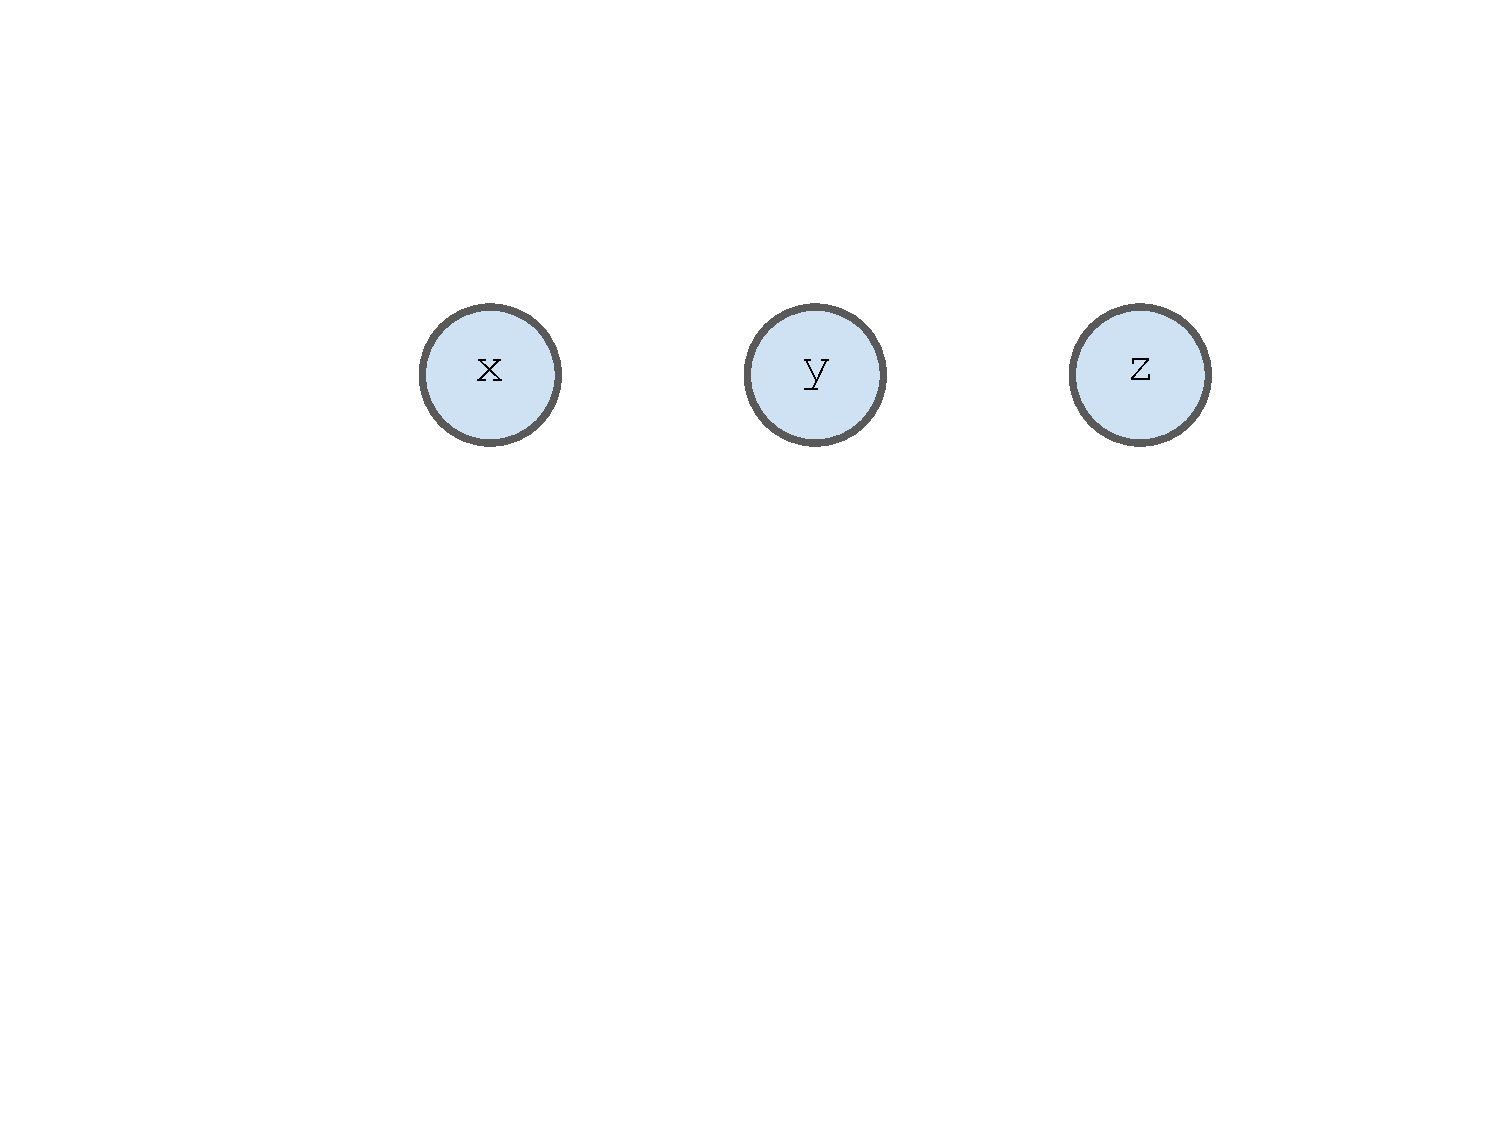
\includegraphics[trim={35mm 115mm 35mm 51mm},clip,width=0.8\linewidth]{assets/must-data/alias-graph0.pdf}
\end{figure*}

Aliasing can be induced by various program operations (e.g., \relname{Move}, \relname{Load}, and \relname{Store}), as seen in our earlier model. Since we are interested in must-alias, two aliased variables have to point to the same object---their nodes can be merged if a \relname{Move} instruction, \code{x = y}, is encountered:

\begin{figure*}[ht]
\centering
% left bottom right top
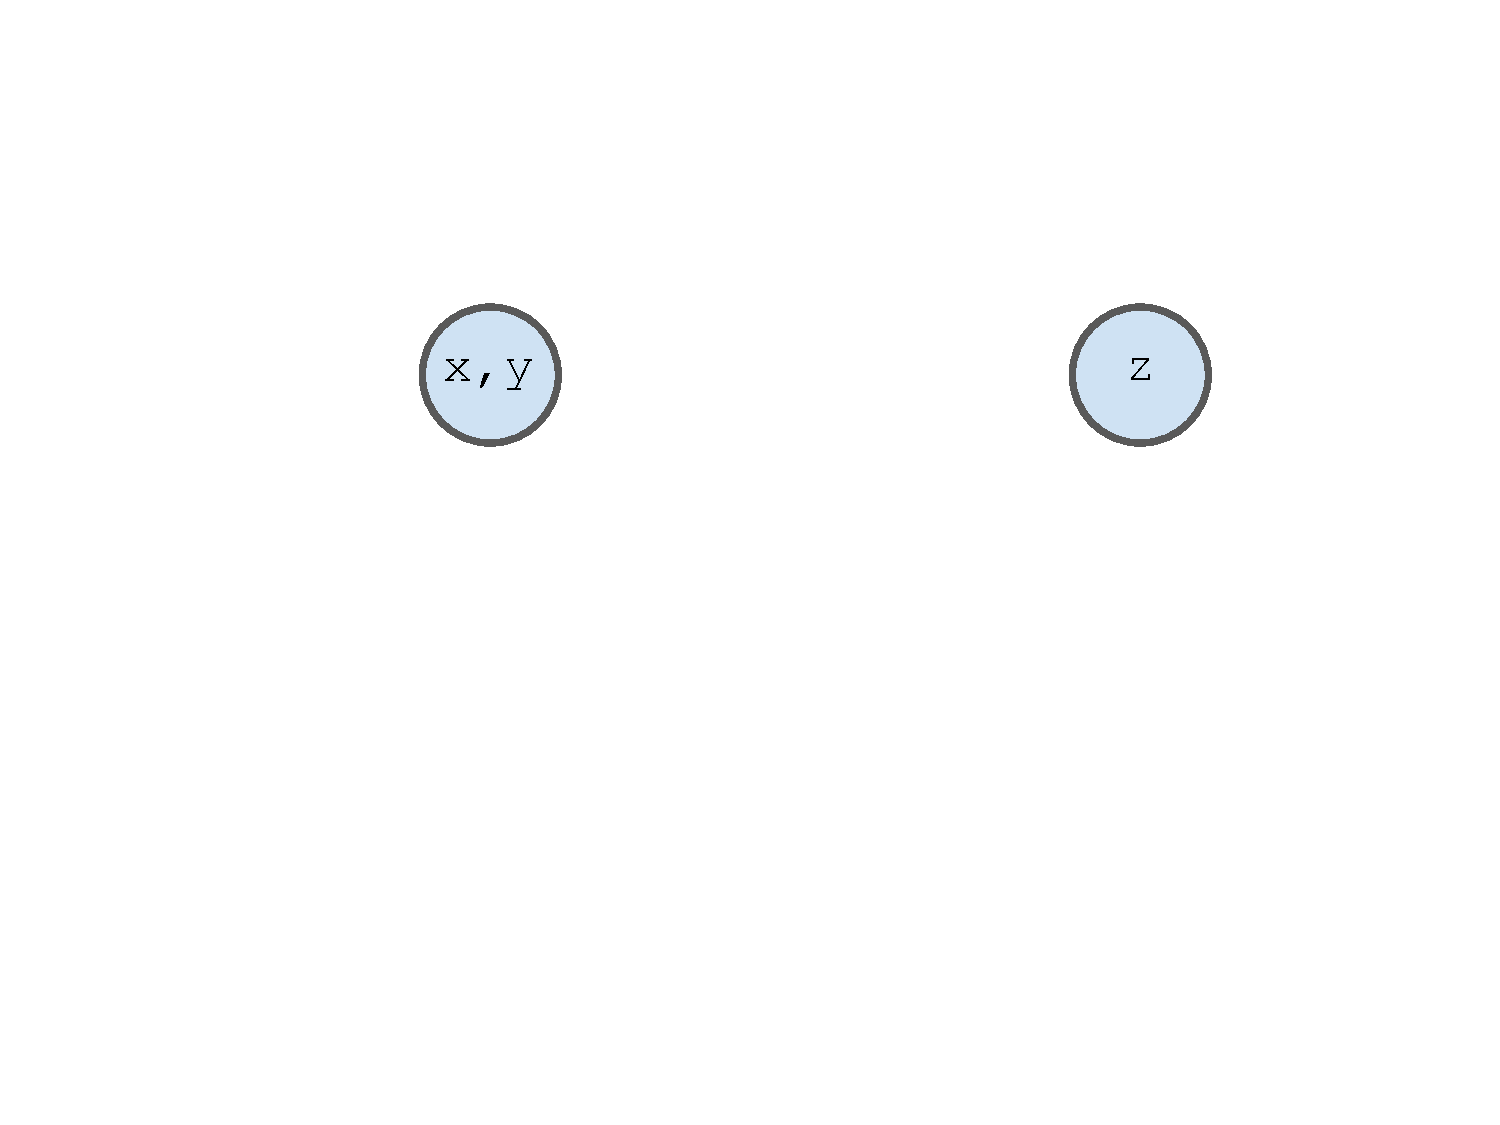
\includegraphics[trim={35mm 115mm 35mm 51mm},clip,width=0.8\linewidth]{assets/must-data/alias-graph1.pdf}
\end{figure*}

This collapsing of nodes is responsible for compact encoding of equivalence relations: two variables are computed to be aliases iff\footnote{The statement refers to the must-alias analysis results, not to actual aliasing during program execution.} they belong in the same node of the alias graph.

If the next instruction is a \relname{Store}, \code{x.f = z}, the previous graph will get propagated---i.e., copied. Subsequently, the \relname{Store} will add an edge to the graph, signifying that the field, \code{f}, of the object pointed by \code{x} will point to the object that \code{z} points to:

\begin{figure*}[ht]
\centering
% left bottom right top
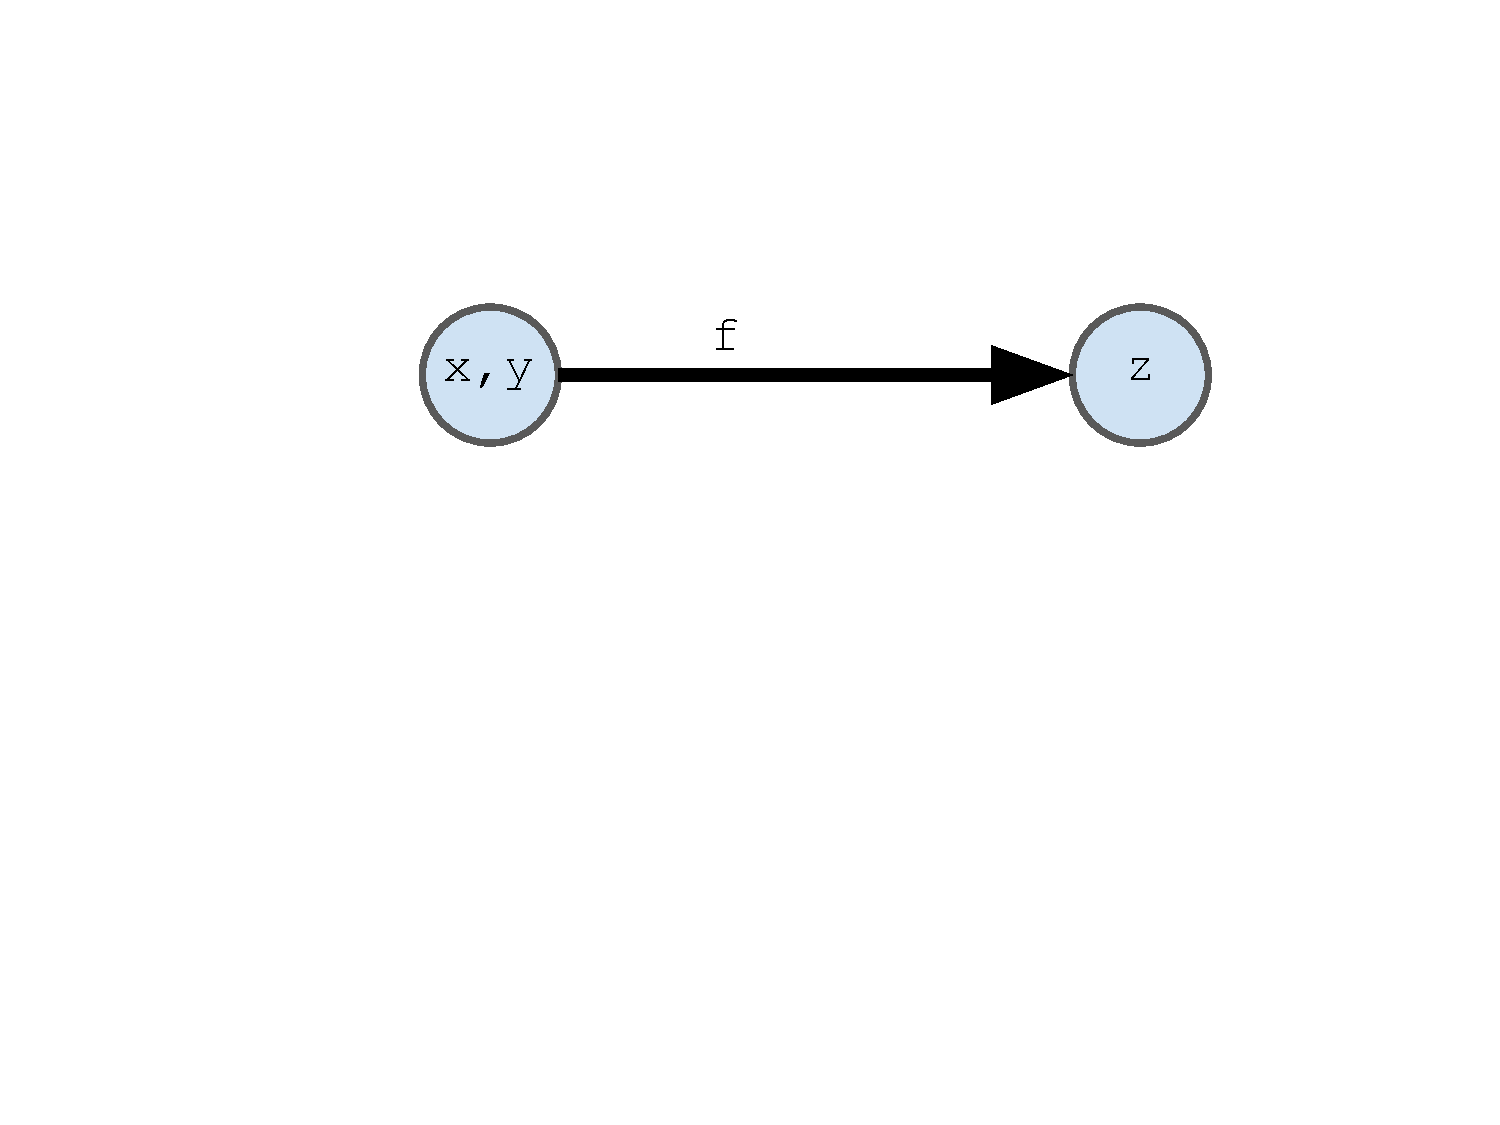
\includegraphics[trim={35mm 115mm 35mm 51mm},clip,width=0.8\linewidth]{assets/must-data/alias-graph2.pdf}
\end{figure*}

A subsequent \relname{Load} operation, \code{z = y.g},\footnote{The example sequence of actions described is contracted for brevity. Our implementation works on a static single assignment (SSA) intermediate form, so this exact scenario will never arise, since \code{z} has had its value read earlier and its single assignment has to dominate its use.} will inherit the alias graph of its predecessor and will modify it. Variable \code{z} is removed from its old node (\code{z} no longer points to this abstract object), a new node for \code{z} is created, and the nodes are linked, to indicate that \code{z} now points to the same object as \code{y.g}. The empty, former node of \code{z} will be garbage collected if no other paths can reach it in the alias graph.

On the other hand, when an access path can still reach the empty node, the empty node provides useful information. It represents ``the object that an access path points to at this program point''. Empty here doesn't describe the lack of information---just the lack of a \emph{local variable} pointing to this abstract object.

\begin{figure*}[ht]
\centering
% left bottom right top
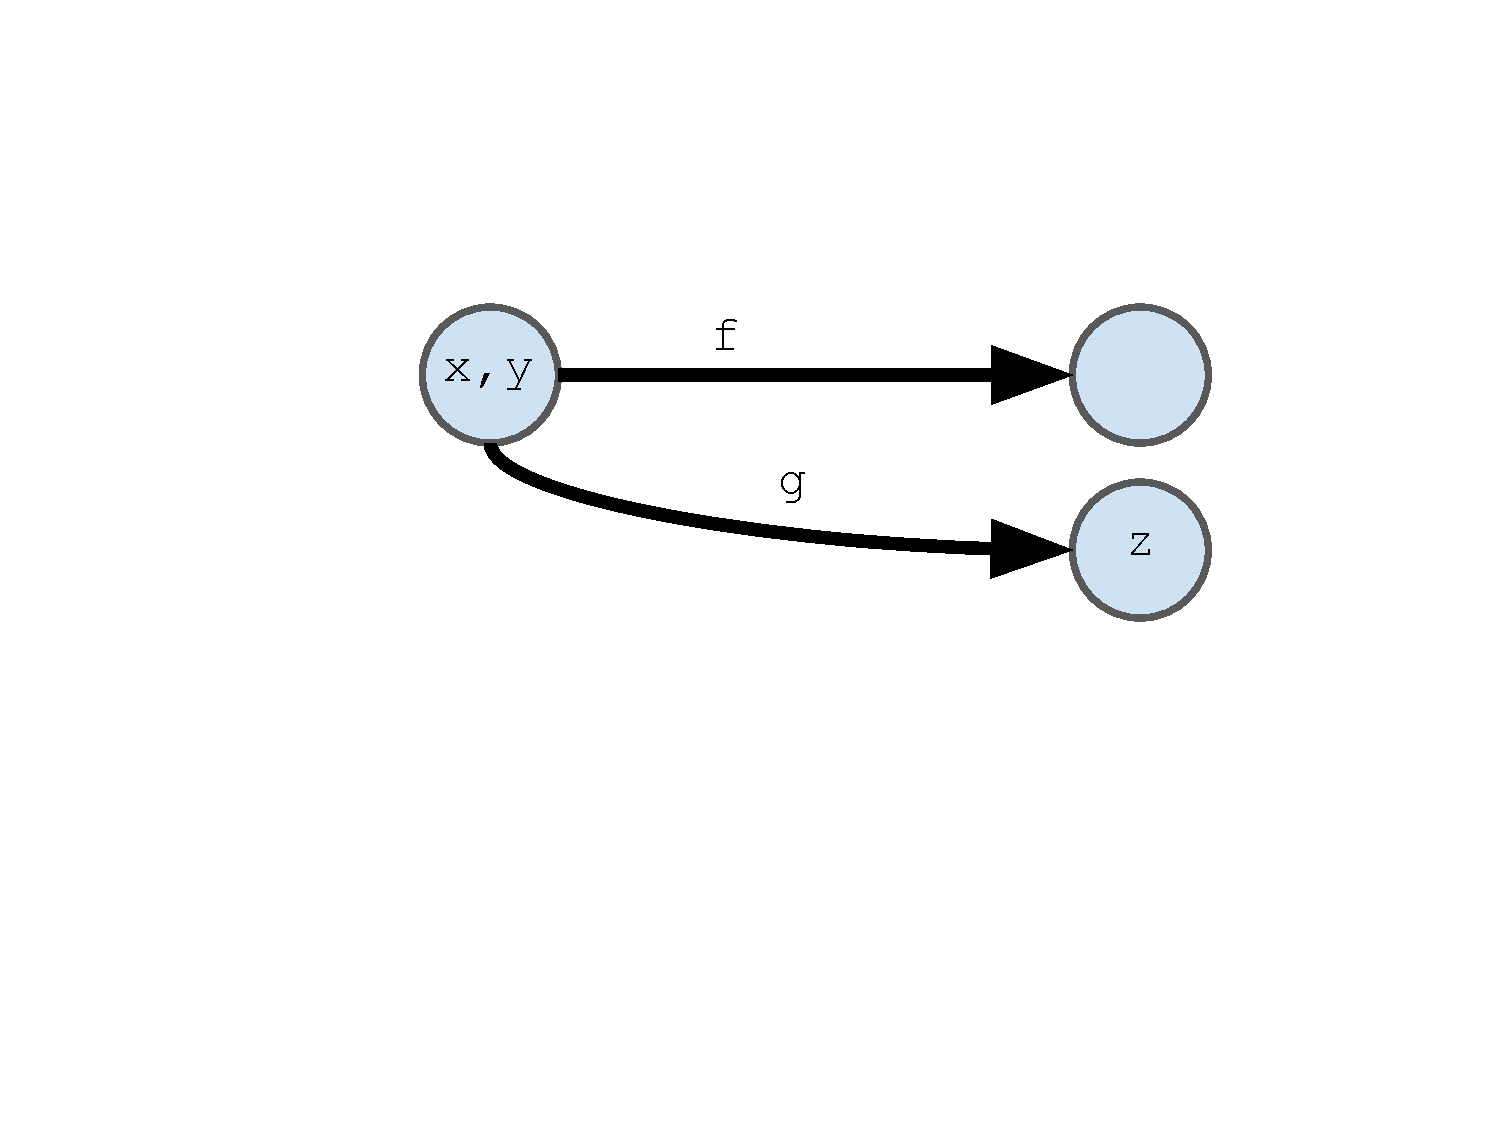
\includegraphics[trim={35mm 85mm 35mm 51mm},clip,width=0.8\linewidth]{assets/must-data/alias-graph3.pdf}
\end{figure*}

The \relname{Load} operation shows that our alias graph, although intended to abstractly represent a real heap, behaves quite differently: a load from a field can introduce new objects, as well as update fields of existing objects.

Generally, the alias graph captures compactly all aliasing relationships among access paths. Maintaining the graph across program instructions is simple, as in the above examples. Graph manipulation merely has to observe some invariants:

\begin{itemize}
\item Two variables are in the same graph node iff the analysis reports them to be aliased. (Since alias classes are disjoint, the variables in different nodes are also disjoint.)

\item A path in the graph represents a set of access paths, starting from a non-empty node (that denotes the base variables of the access paths) and extended with the field labels along the path's edges. If two paths in the graph reach the same node, all access paths they represent must be aliased.
\end{itemize}

For illustration, consider Figure~\ref{fig:must-data:alias-graph}, which shows the alias graph after line 19 of our code example in Figure~\ref{fig:must-data:snippet}.

\begin{figure}[ht]
\centering
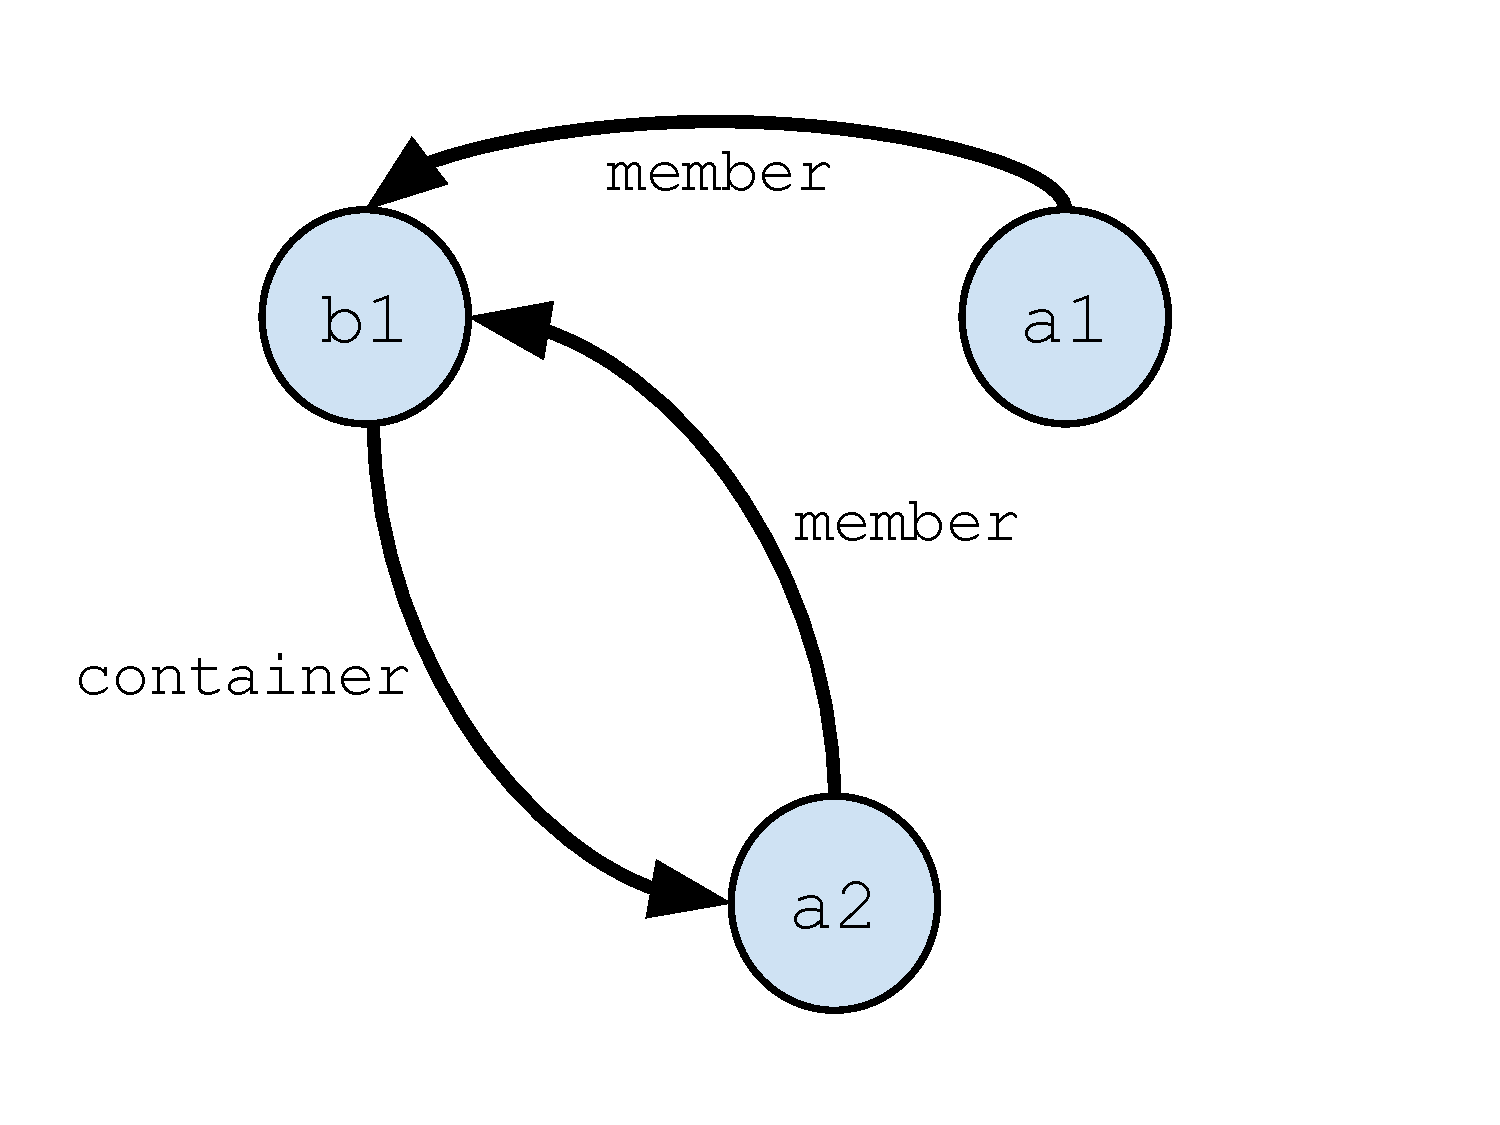
\includegraphics[trim={13mm 15mm 10mm 10mm},clip,width=0.7\linewidth]{assets/must-data/alias-graph.pdf}
\caption{Example alias graph data structure.}
\label{fig:must-data:alias-graph}
\end{figure}

The graph concisely represents a set of alias relationships that hold at that program point: \{\code{b1.container} $\sim$ \code{a2}\}, \{\code{a1.member} $\sim$ \code{b1}\}, and \{\code{a2.member} $\sim$ \code{b1}\}. An infinite number of other alias pairs are represented implicitly: \{\code{a1.member} $\sim$ \code{a2.member}\}, \{\code{a1.member.container} $\sim$ \code{a2}\}, \{\code{a1.member.container.member} $\sim$ \code{b1}\}, \{\code{a1.member.container.member} $\sim$ \code{a1.member}\}, etc.

Overall, the alias graph satisfies both of our requirements of Section~\ref{sec:must-data:needs} for an efficient representation. Equivalence relations are represented compactly: an alias class with $n$ members does not need $O(n^2)$ space and time for its computation. Instead, it is represented implicitly, as all the variables in a node ($O(n)$ space) and all alias graph paths that can reach a node. Similarly, long (and even infinite) access paths are represented implicitly as graph paths. The implicit representation is sufficient for any specific queries (i.e., ``are two given program expressions aliases?'') and for subsequent aliasing computations, per the algorithms we detail next.


\subsection{Main Algorithms}

Most of the required must-alias analysis actions (per the discussion of Section~\ref{sec:must-data:needs}) over our data structure are straightforward, consisting of copying, additions and removals of variables and edges, and variable renamings. Standard mappings for efficient indexing are required: each target of a directed edge needs to be able to quickly retrieve its source, and each program variable needs to quickly map to the node in which it appears. 

For instance, according to the earlier definition of the data structure, finding all aliases of an access path is simple (but requires a transitive computation---our graph is a condensed representation of alias classes):


\paragraph{Algorithm: \rel{all-aliases}{ap}}
\begin{itemize}
\item Find the node for the base variable of access path \args{ap}, traverse in the forward direction the labeled edges that match each of the fields of \args{ap} to reach a target node.

\item Any graph path that reaches the same node corresponds to an aliased access path, from a base variable adding the fields labeling the edges. (I.e., traverse $k-1$ directed edges backwards to find access paths of length up to $k$.)
\end{itemize}

For instance, in Figure~\ref{fig:must-data:alias-graph}, we can find all aliases of length 3 of access path \code{a2.member} by traversing edge \code{member} from node \code{a2} (thus reaching the node containing \code{b1}) and finding all paths of length 2 that can reach the same node, also including the variable(s) in the starting node of the path (e.g., \code{b1.container.member}).

The more interesting algorithm, as suggested earlier, is that of intersecting alias graphs---necessary for merging alias information from predecessor instructions. This is easy to see as a repeated intersection of two graphs (which is then iterated by intersecting a third with the result, then a fourth, and so on). Note that the graphs do not need to contain a single connected component.


\paragraph{Algorithm: \rel{intersect}{g1, g2}}
\begin{itemize}
\item The domain of possible nodes for the result of the intersection is the cartesian product of nodes of \args{g1} and \args{g2}. For every two nodes $i$, $j$ of \args{g1} and \args{g2}, respectively, node $(i,j)$, if it exists in the intersection result, will contain the intersection of the variables of $i$ and $j$.

\item Nodes are materialized incrementally, according to the rules below.
\begin{enumerate}
    \item For every two nodes $i$, $j$ of \args{g1} and \args{g2}, if the intersection of the variables of $i$ and $j$ is non-empty, add to the intersection result a new node $(i,j)$.

    \item (Repeatedly) If node $(i,j)$ exists in the intersection result, then for every label $f$, if \args{g1} has an edge $i \rightarrow k$ with label $f$, and \args{g2} has an edge $j \rightarrow l$, also with label $f$, then add to the intersection result (if not already present):
    \begin{itemize}
        \item[-] a node $(k,l)$ (possibly empty);
        \item[-] an edge $(i,j) \rightarrow (k,l)$ with label $f$.
    \end{itemize}
\end{enumerate}
\end{itemize}

Note that the first step is of linear complexity in the number of nodes, since empty nodes can be eagerly skipped and indexing from a variable to the, up to one, node that may contain it in a different graph is constant-time.

The algorithm considers all possible pair-wise node combinations and all possible edges out of node intersections. It maintains the property that any aliasing relationship (either variables belonging in the same node, or paths reaching the same node) in the result also exists in both input alias graphs.

Notably, the intersection of two alias graphs can produce nodes with empty variable sets, due to the second step of the algorithm. Empty nodes with no in-edges can be eliminated eagerly. Empty nodes with in-edges are meaningful in the output and need to be maintained. To illustrate, consider the example in Figure~\ref{fig:must-data:intersection}.

\begin{figure}[ht]
\centering
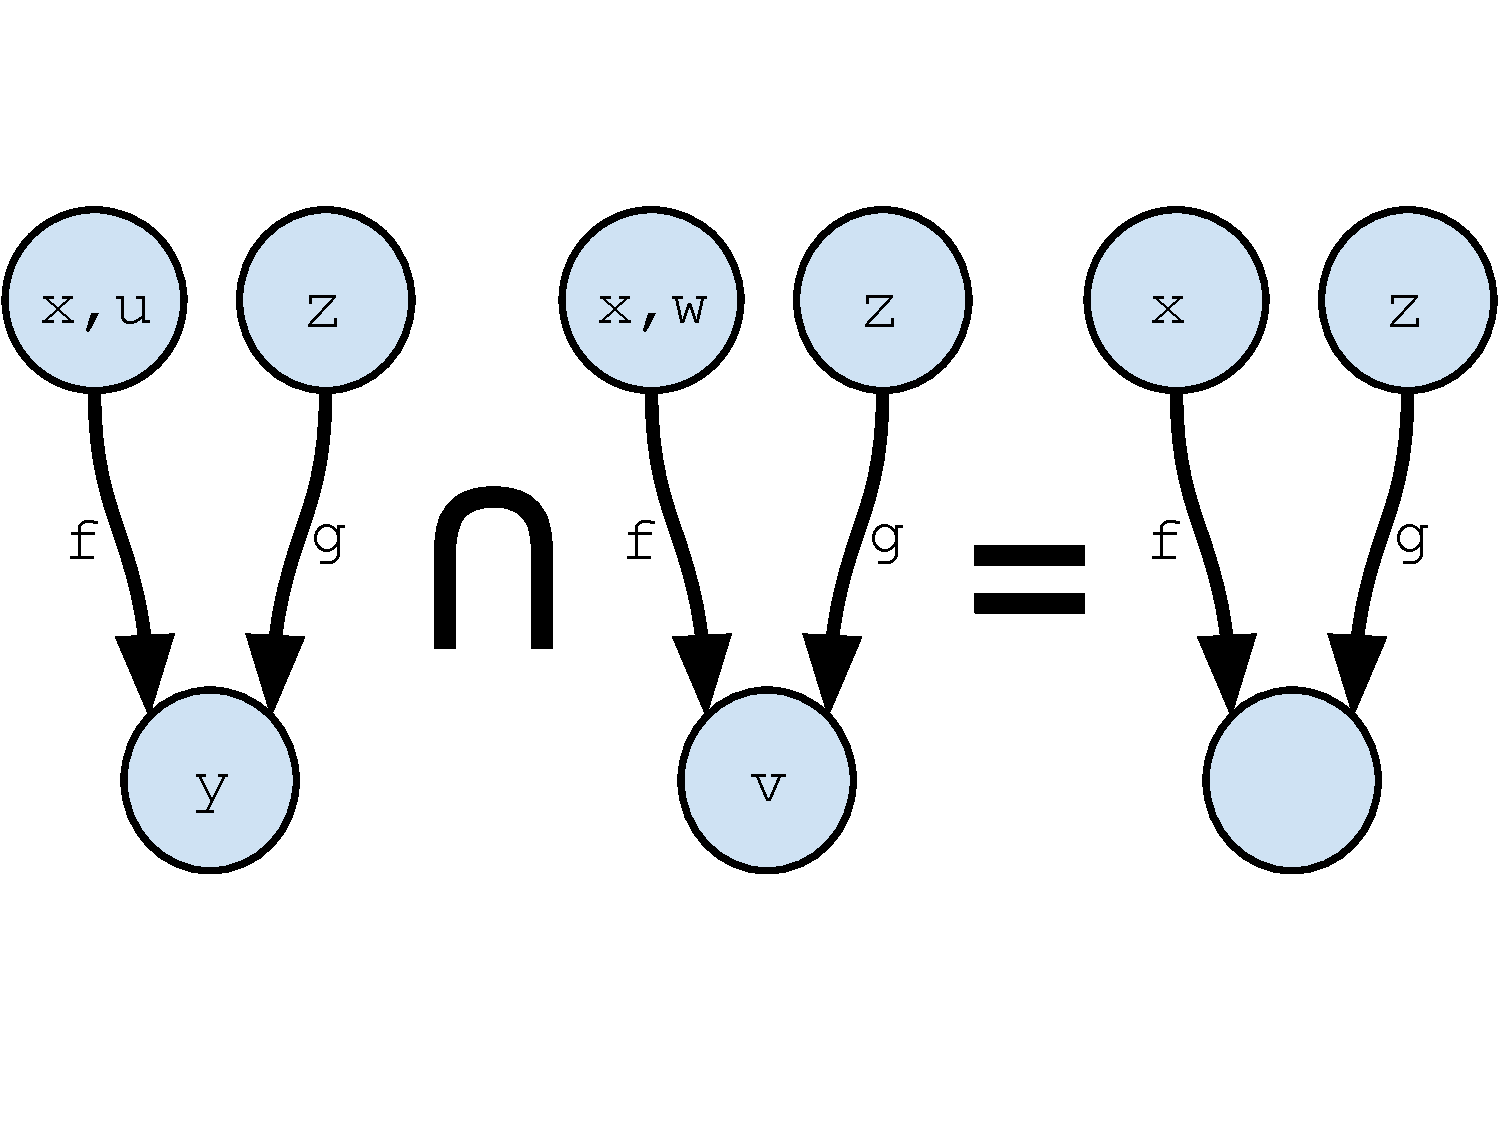
\includegraphics[trim={0mm 40mm 0mm 30mm},clip,width=0.9\linewidth]{assets/must-data/intersecting-alias-graphs.pdf}
\caption{Intersecting alias graphs.}
\label{fig:must-data:intersection}
\end{figure}

In this case, the empty note denotes that access paths \code{x.f} and \code{z.g} are still aliased in the intersection alias graph, even though they are no longer aliased with any single-variable access path.

For upper bounds $n$, $v$, $e$ in the number of nodes, variables, and edges in the input alias graphs, respectively, the algorithm has a running time asymptotic bound of $O(n + v + e)$, i.e., linear in all
quantities, if one assumes a practically constant-time indexing scheme from a variable to its node. (\textbf{Proof sketch}: Non-empty nodes are fewer than variables and only linear cost is incurred when combining non-empty nodes pair-wise, since each node has a distinct set of variables, used to index into any node that may intersect that set in the other alias graph. Empty nodes arise in the result and are only examined in the input if there is an edge into or out of them, therefore their number is below $e$. The number of edges in the output is at most that in the input---taken as the union of both input graphs).

Empty nodes with no in-edges are only one instance of nodes that no longer encode useful access path aliasing. Such nodes should be garbage-collected for maximum efficiency, producing a normalized input. The node collection algorithm is as follows:


\paragraph{Algorithm: \rel{gc}{g}}
\begin{itemize}
\item Any node in \args{g} containing a single variable and with no incoming or outgoing edges is eliminated.

\item Any node in \args{g} containing no variables and with either zero in-edges or one in-edge and zero out-edges is eliminated.
\end{itemize}

In all cases covered by the above algorithm, the node does not encode alias pairs that would disappear with the node's removal: either there are no two paths (or variable names) that reach the node, or the node does not extend other paths beyond the implicit extension with the same field names that is already captured by the data structure.


\subsection{Use in Practice}

Having described the individual steps of an analysis using a must-alias data structure, we turn our attention to how it is used in the context of a realistic analysis. Consider the must-alias analysis of the \doop{} framework, discussed in Chapter~\ref{chapter:must-logic}. This computes a \rel{MustAlias}{i, ctx, ap1, ap2} relation, i.e., aliased access paths at each program point and calling context. That is, each instruction-and-context combination is associated with an alias graph. Initially, conceptually every possible variable has its own node. (Implementation-wise, this is represented as an empty graph, requiring no initialization.) Every program instruction is visited and its alias graph is updated based on the instruction semantics and the operations that we described earlier. Specifically, every variable-aliasing instruction merges nodes (creating them if they only existed implicitly, i.e., they were single-variable nodes), every load and store instruction creates nodes and/or edges, every instruction also integrates the alias graphs of its predecessors, intersecting them if the instruction is a control-flow merge point. The visit order is not important for correctness, though it might affect performance (i.e., the number of steps needed before convergence is achieved).

At a call instruction, the analysis creates a new instruction-and-context pair (unless it exists already) for the first instruction of the callee method and the given context. Maximum context depth is a parameter of the analysis and if reached the call instruction will not be further analyzed. This is a sound approach for a must-alias analysis, since the aim is to compute an \emph{under}-approximation of the alias relationships that are guaranteed to hold. With our data structure, the alias graph at the call site is copied to the first instruction in the callee method and then the usual operations are applied.

The above are repeated until a fixpoint is met. At any given alias graph, the number of non-empty nodes is bounded by the number of local variables in the program text. Empty nodes can arise but \relname{gc} ensures that the intersection operation, where merging of states takes place, can never produce more modes than the union of its inputs graphs: if an empty node is kept, it is because an incident edge existed in the input, hence a corresponding node appeared in the input.


\subsection{Declarative Implementation}

As discussed earlier, the alias graph data structure can be employed in a must-alias analysis by maintaining alias graphs per-program-point (i.e., per context-qualified instruction), and updating them (to incorporate information from their predecessor instructions) until fixpoint.

The data structure description we have seen so far considers this update to be a destructive operation. For instance, after a \relname{Move} instruction, we saw the nodes of two variables getting merged. Similar merging can be induced by information that the analysis discovers while it is executing (i.e., not directly induced by the semantics of the current instruction)---e.g., propagated from predecessors.

We have also designed and implemented a declarative/purely functional version of the data structure. The main reason for the declarative implementation has been fairness in experimental comparisons. We will compare our optimized implementation against the must-alias analysis of the \doop{} framework, implemented in Datalog. Thus, it is desirable to also implement a, perhaps not as optimal, declarative version of the data structure in Datalog. This will allow us to isolate the effect of destructive updates from the inherent properties of the data structure.

In the declarative version of the structure, aliased abstract objects are not merged, but instead associated with each other. Schematically, we can consider that each variable has its own node and points to at least one abstract object---at first the abstract object signifying ``whichever object the variable got assigned to'' (at its single-assignment site):

\begin{figure*}[ht]
\centering
% left bottom right top
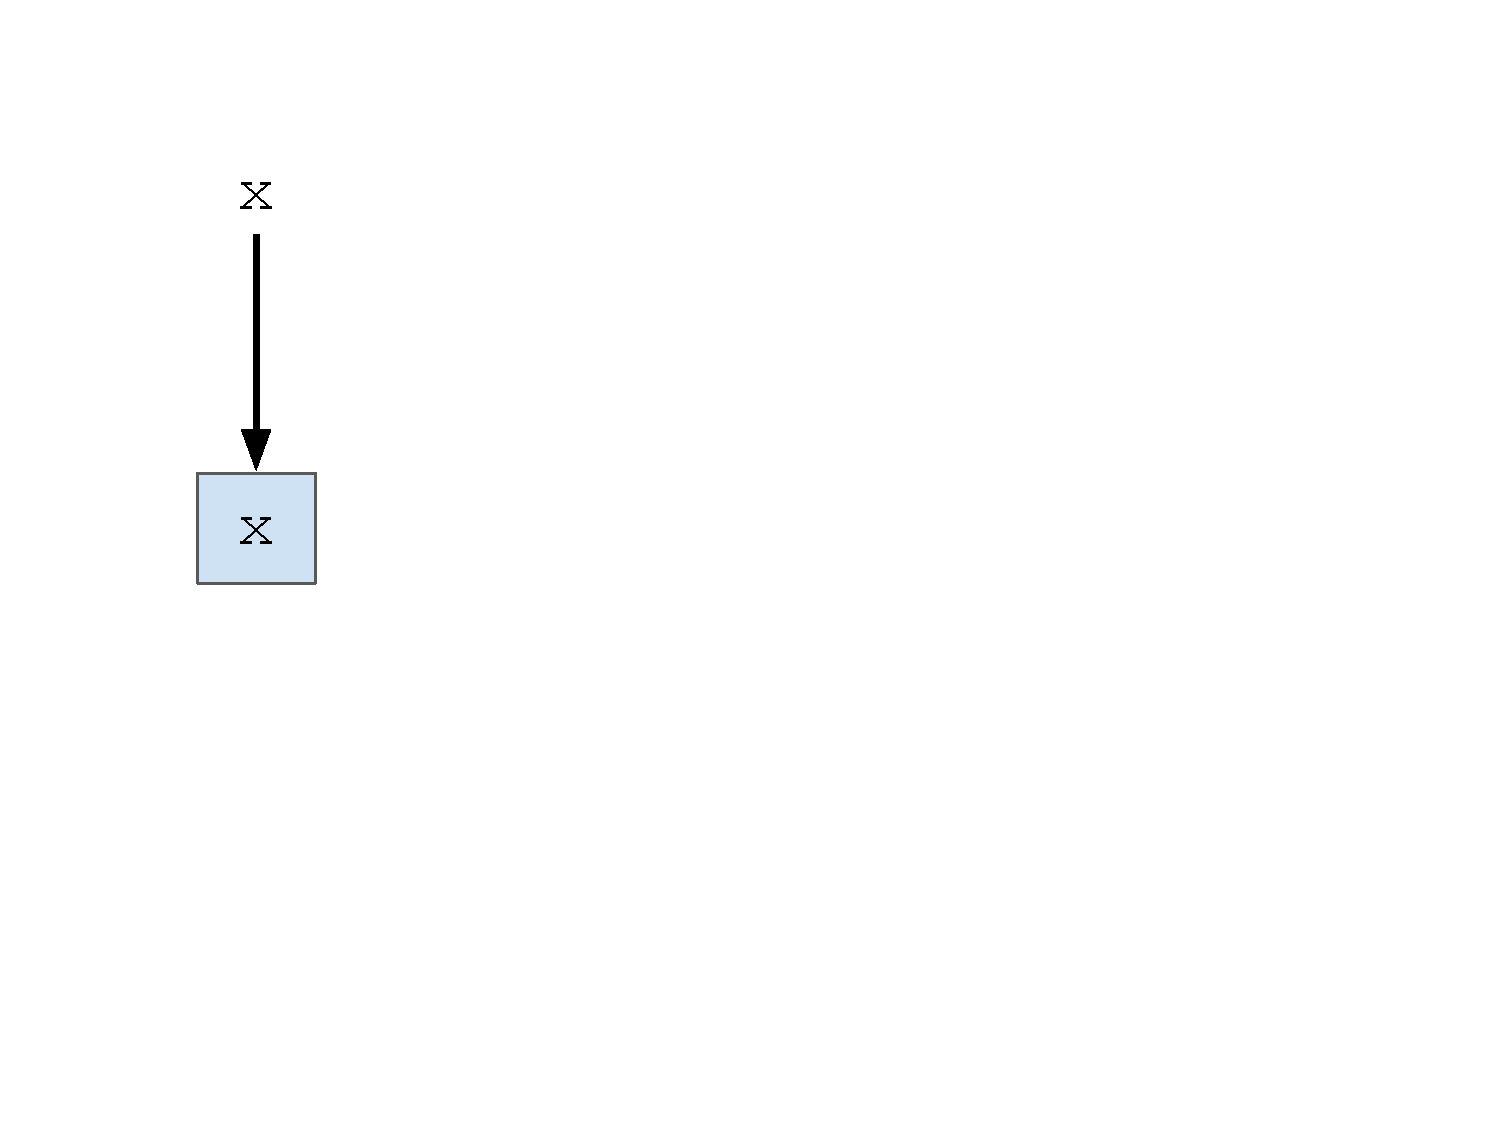
\includegraphics[trim={25mm 90mm 190mm 25mm},clip,width=0.15\linewidth]{assets/must-data/decl-alias-graph0.pdf}
\end{figure*}

(For the declarative implementation, we will represent abstract objects as squares, to avoid confusion.)

Since we no longer have destructive updates, variables can point to multiple abstract objects. For instance, after a \relname{Move} instruction, \code{x = y}, we have:

\begin{figure*}[ht]
\centering
% left bottom right top
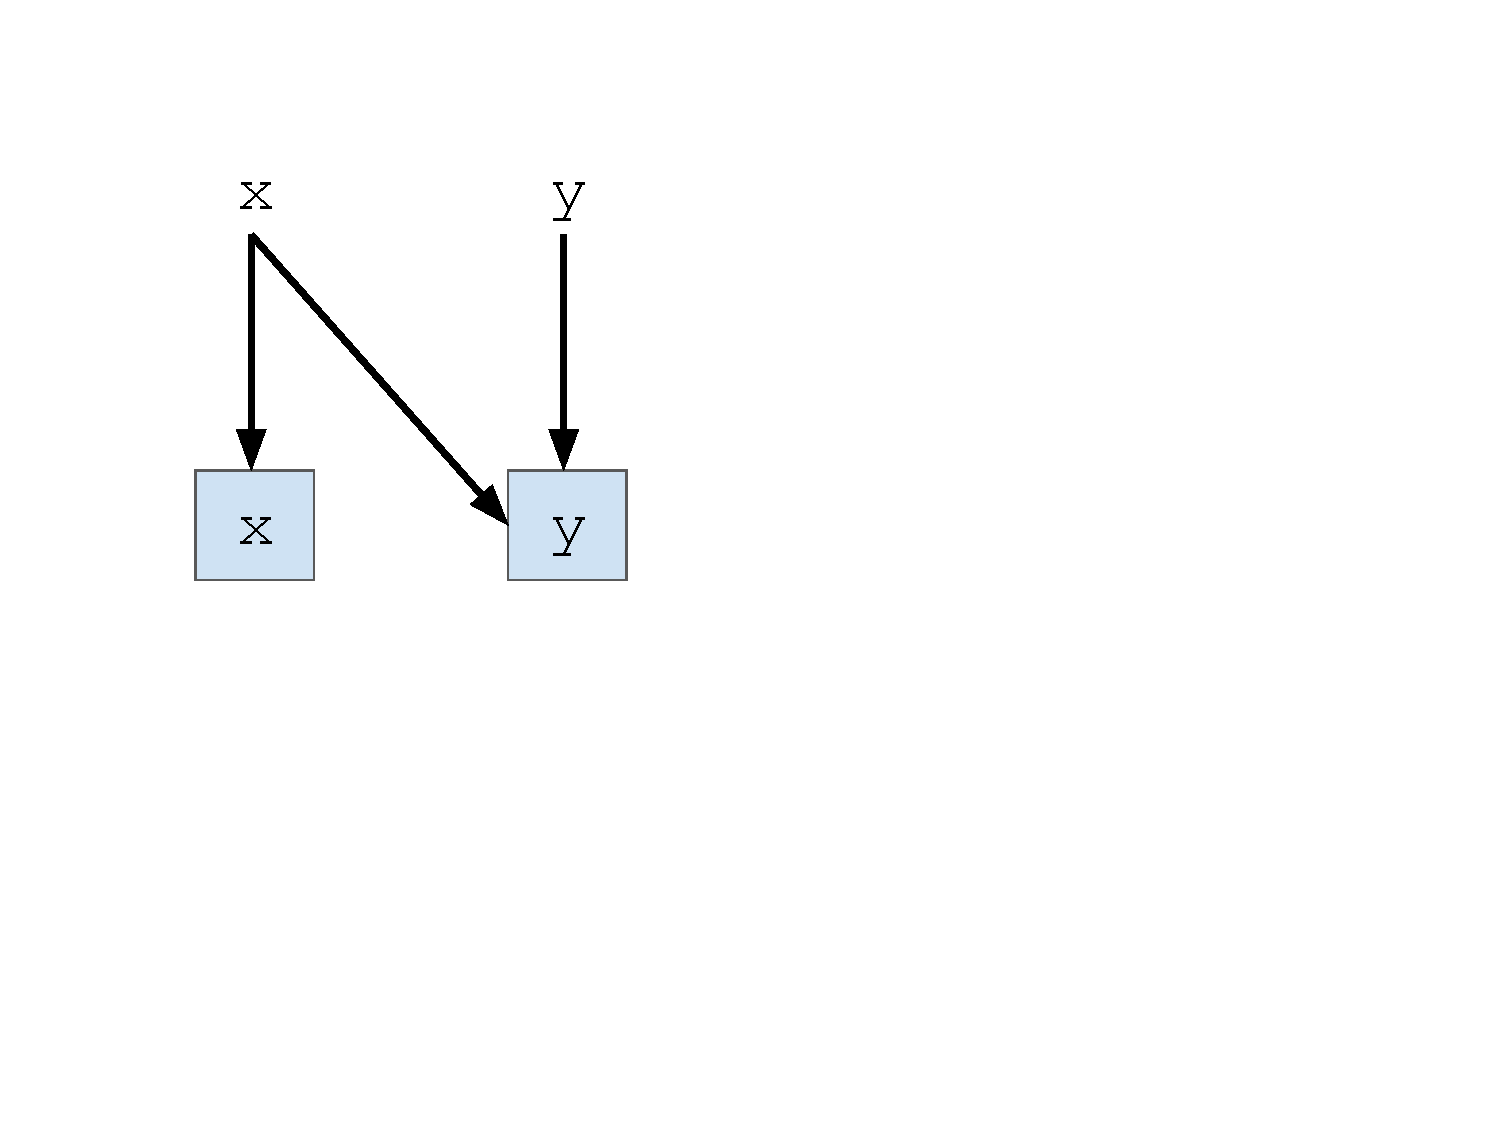
\includegraphics[trim={30mm 90mm 140mm 25mm},clip,width=0.32\linewidth]{assets/must-data/decl-alias-graph1.pdf}
\end{figure*}

As before, however, a variable can really point to a single concrete object. Therefore, the two abstract objects that \code{x} points to have to be different abstractions of the same concrete object---their equivalence is encoded, but implicitly. It is easy to check that variables \code{x} and \code{y} are aliased, in the usual sense: they both point to the same abstract object.

If the next operation is another \relname{Move}, \code{z = x}, variable \code{z} is made to point to both abstract objects that \code{x} points to:

\begin{figure*}[ht]
\centering
% left bottom right top
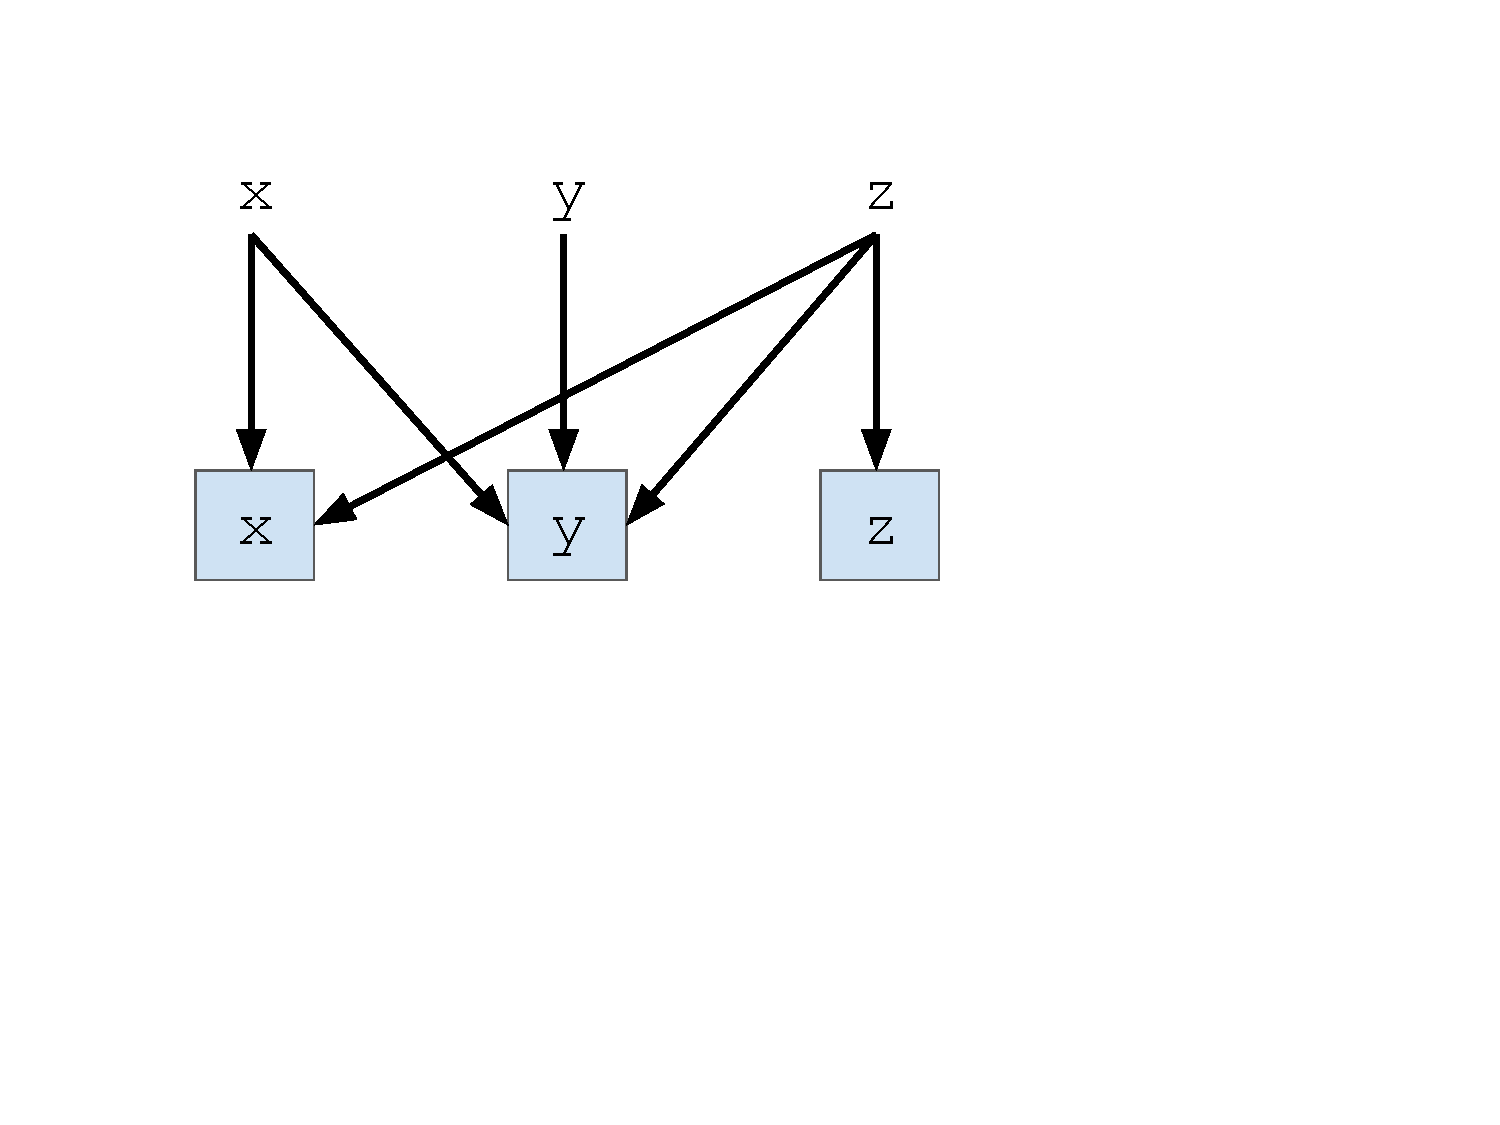
\includegraphics[trim={25mm 85mm 70mm 25mm},clip,width=0.6\linewidth]{assets/must-data/decl-alias-graph2.pdf}
\end{figure*}

Thus, the declarative data structure is less efficient than its imperative counterpart: a quadratic representation of an alias set cannot be precluded, and depends on the order of alias-inducing instructions. In our example, we could then assign \code{z}, the variable with the most out-edges, to a new variable, \code{w}, then assign \code{w} (which now has the most out-edges) to a new variable, and so on. In practice we expect that this effect will be mitigated. If the next instruction assigns \code{y} to a new variable, \code{u}, then \code{u} receives only a single extra edge, maintaining a more compact representation of the alias set. The cost, much as in the imperative structure, is that the alias set is not fully explicit and requires a transitive closure computation to be materialized.


\section{Evaluation}

We implemented an analysis that functionally matches the one present in the \doop{} framework that is implemented in Datalog (whose core ideas are aptly captured in the model of the previous chapter). In contrast, our implementation is in Java, since our optimized alias graph data structure has imperative features in its full form. Finally, to also eliminate language-level factors of the Datalog-vs-Java implementations, we also produced an optimized Datalog implementation, based on our purely functional data structure.

The three implementations are functionally equivalent, with very minor variations, due to clear engineering differences: The original Datalog analysis has to bound the access path length for aliases to a finite number, while the optimized data structure implicitly stores aliases for longer access paths. This may allow inferring more aliases even for shorter access paths. Also, for engineering simplicity, the Java implementation incorporates just a naive fixpoint computation. In each fixpoint iteration, it keeps track of a set of instructions whose alias graphs might be affected by the current changes, and those are the instructions that will be inspected in the next iteration. This process is repeated until there are no further instructions for consideration. The fixpoint computation is only crudely tuned for performance and the algorithm is eager to mark an instruction as a candidate for the next iteration.

Since the analyses are virtually equivalent, we next compare them only on speed. (For context, however: the analysis is quite effective and computes far from trivial results. It produces enough must-alias inferences to determine unique points-to targets for 20-40\% of local variables in all benchmarks. Its current main uses inside \doop{} are to enable strong updates in a may-point-to analysis, as well as to produce results for inspection by humans, to aid program comprehension.)

We use a 64-bit machine with an Intel(R) Xeon(R) E5-2687W v4 (24-cores) CPU at 3.00GHz. The machine has 512GB of RAM. All measurements are single-threaded (though, as is common, Java runs its garbage collector in extra threads) and all executions occupy only a small fraction of the available RAM. We experiment with the DaCapo benchmark programs~\cite{oopsla:2006:Blackburn} v.2006-10-MR2 and v.9.12-bach under JDK 1.7.0\_45.  We use the LogicBlox Datalog engine, v.3.10.14.


\paragraphhead{Speed across benchmarks.}
Figure~\ref{fig:must-data:time-chart} shows the performance effect of our optimized data structure on analyzing the benchmark programs. We bounded the access path length (for the original Datalog analysis) to 3 and the analysis context depth to 2.

\begin{figure*}[htp]
\centering
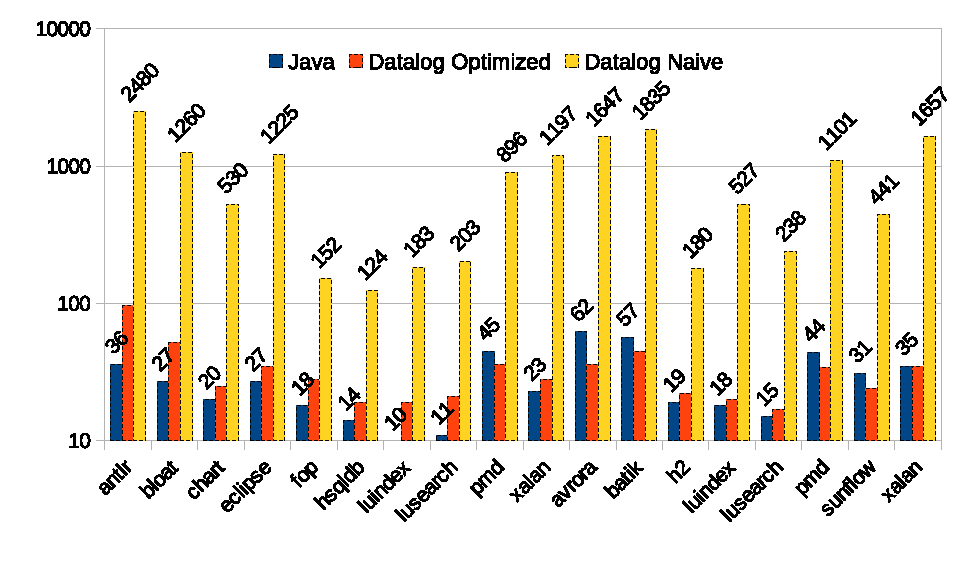
\includegraphics[clip,width=0.77\linewidth, height=0.4275\linewidth]{assets/must-data/time.eps}
\caption{Execution time (sec.) of the analysis. We only show the numbers for the Java and Datalog naive versions, to avoid crowding the chart.}
\label{fig:must-data:time-chart}
\end{figure*}

Note that the figure is log-scale. Across all benchmarks, the difference between the optimized implementations and the original is typically at least an order of magnitude and often close to two.  The speedup of the two optimized implementations (vs. the original) is also shown more explicitly in Figure~\ref{fig:must-data:speedup-chart}: over half the benchmarks enjoy speedups of over 20x for both the Java and the Datalog optimized implementation. The Java version of the data structure achieves a median speedup of 25.7x (min. 8.4x, max. 68.9x), while the Datalog version has a median speedup of 24.6x (min. 5.4x, max. 47.3x).  The analysis time typically drops from over ten minutes to under half a minute. 

\begin{figure*}[htp]
\centering
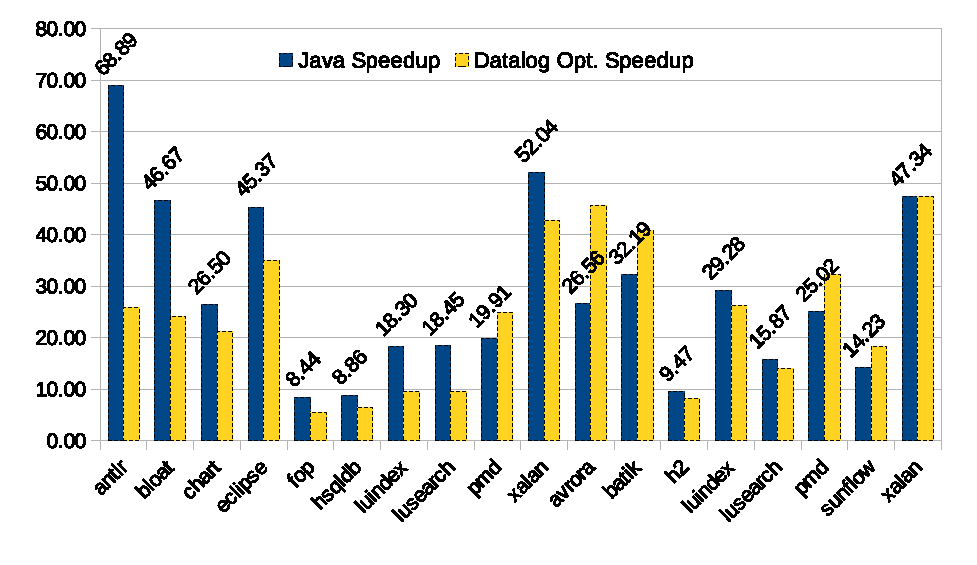
\includegraphics[clip,width=0.77\linewidth, height=0.4275\linewidth]{assets/must-data/speedup.eps}
\caption{Speedup of the two analyses employing optimized data structure.}
\label{fig:must-data:speedup-chart}
\end{figure*}

It is not hard to see why the explicit representation is not competitive. Figure~\ref{fig:must-data:pairs-chart} correlates the number of aliased access-path pairs (computed by the original analysis) and execution time. (This applies to context-qualified access paths, in the application and libraries alike, as long as the library code is reachable from application code with the given context depth.) This metric reflects the size (in tuples) of the corresponding relation in the Datalog database. It clearly suggest that maintaining access path relationships explicitly can prove quite costly.

\begin{figure*}[htp]
\centering
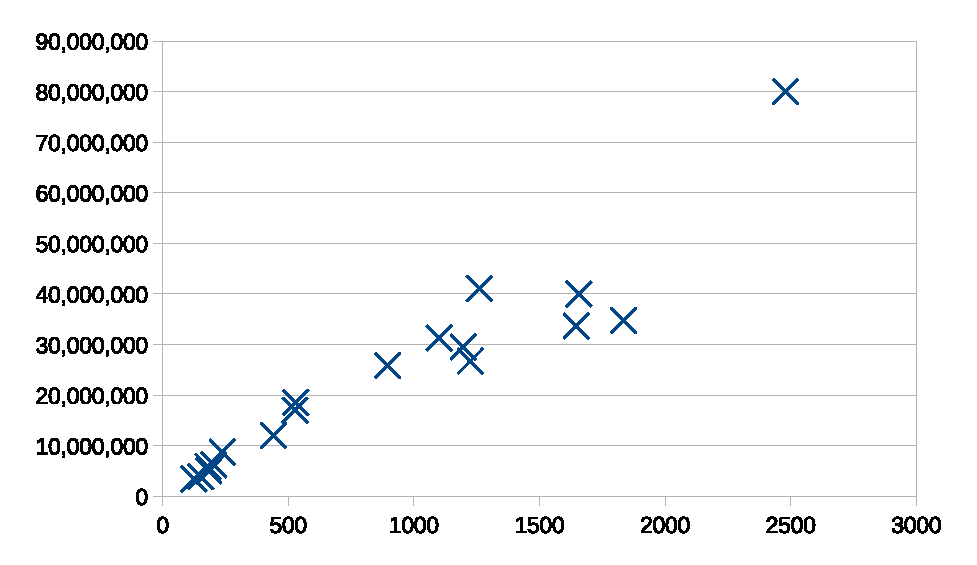
\includegraphics[clip,width=\linewidth]{assets/must-data/pairs.eps}
\caption{Number of pairs of (instruction-and-context qualified) access paths that must alias vs. analysis time.}
\label{fig:must-data:pairs-chart}
\end{figure*}

Furthermore, the setup explicitly downplays the benefits of our optimized data structure: First, the ``optimized'' running time also includes import time and computing must-point-to results for checking the equivalence of analyses. The latter is quite costly, since it requires re-expanding the compactly-preserved access paths. The true computation times of the optimized analysis are about one-third of the times listed in Figure~\ref{fig:must-data:time-chart}. Second, the configuration parameters (context depth of 1 and access paths of at most length 2) are very modest, to present the explicit representation in the best possible (while still realistic) light. Changing these parameters can incur dramatic slowdowns for the explicit representation, as we examine next.


\paragraphhead{Varying access-path length.}
To further see the performance advantage of the optimized representation of must-alias information, one can vary the maximum access path length allowed for computations of the original, explicit (Datalog) implementation. Figure~\ref{fig:must-data:aplength-chart} shows how running time varies for maximum access path lengths of 2, 3 (same as in Figure~\ref{fig:must-data:time-chart}), 4 and 5. The numbers are for the xalan benchmark. The speedup readily grows to over 75x for an allowed access path length of 5. The optimized Datalog implementation is shown as a baseline although it should be (and is) largely unaffected by the change of maximum access path length.

\begin{figure*}[htp]
\centering
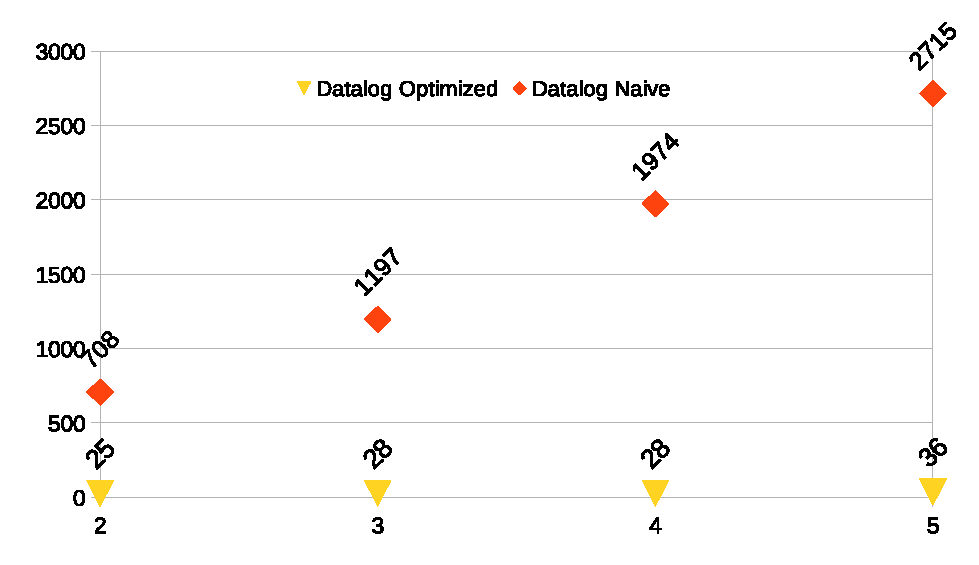
\includegraphics[clip,width=\linewidth]{assets/must-data/length.eps}
\caption{Execution time when varying maximum access-path length. Optimized Datalog running time given as a baseline.}
\label{fig:must-data:aplength-chart}
\end{figure*}


\paragraphhead{Varying context depth.}

\begin{figure*}[h!tp]
\centering
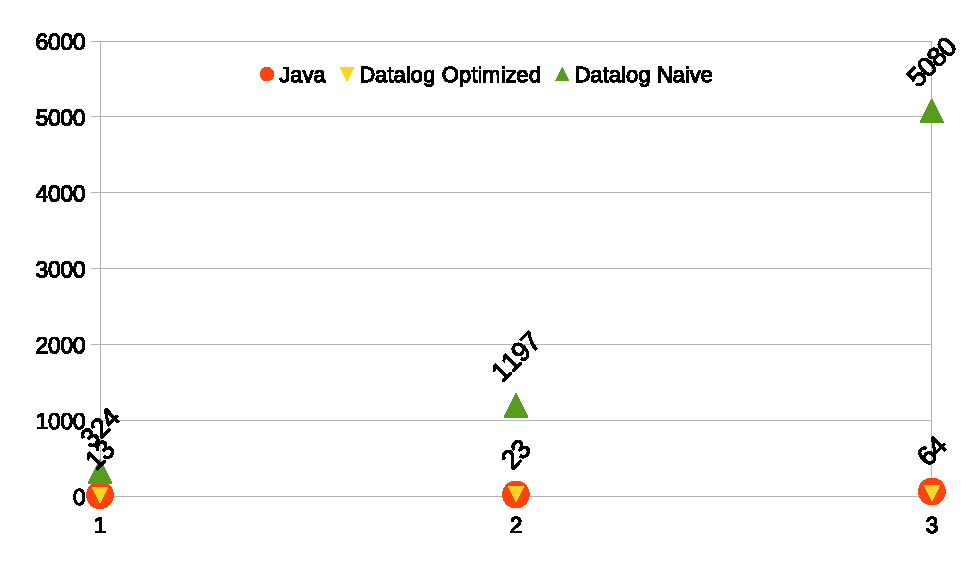
\includegraphics[clip,width=\linewidth]{assets/must-data/depth.eps}
\caption{Execution time when varying maximum context depth.}
\label{fig:must-data:ctxdepth-chart}
\end{figure*}

Similar observations can be made by varying the context depth of the analysis. As seen in Figure~\ref{fig:must-data:ctxdepth-chart}, although the running time of the optimized implementation grows slowly, the running time of the explicit representation of alias relationships gets dramatically higher. For a context depth of 4, the explicit representation did not terminate after one-and-a-half hour.

Recall the two claimed benefits of the optimized representation: long access paths are represented implicitly, and equivalence classes are represented with linear space and time complexity, instead of quadratic. It is the latter factor that comes into play when context depth increases: alias sets grow in size, by exploiting inter-procedural inference (e.g., aliasing established at the caller and propagated through formal arguments) in addition to local instructions.


\section{Summary}

We presented a data structure for the its optimized implementation of must-alias analysis over access paths. In all, the optimized representation fulfills its promise of a much more economical representation of must-alias (equivalence) relations. The algorithmic improvements afforded by the specialized data structure yield a large performance advantage, often approaching two orders of magnitude.
%\chapter{Defensive Points-To Analysis}
\label{chapter:defensive}
\epigraph{You don’t just give up. You don’t just let things happen. You make a stand!}{\textit{Rose Tyler} - Doctor Who}
%\epigraph{Progress isn't made by early risers. It's made by lazy men trying to find easier ways to do something.}{\textit{Robert Heinlein}}

\emph{Soundness} is a coveted property of static analyses, to the extent that the term is often colloquially used as a synonym for ``correctness''. For a may-analysis, soundness means that the analysis abstraction over-approximates all concrete executions. A sound value-flow or points-to analysis is one that computes, per program point or per variable, value sets that represent (at least) all values that could possibly arise at the respective point during any possible execution.

Full soundness is hard to achieve in practice due to code that cannot be analyzed (e.g., dynamically generated/loaded code, binary/native code) or dynamic language features (e.g., reflection, \code{eval}, \code{invokedynamic}). We collectively refer to such features as \emph{opaque code}. For instance, the Java code below invokes an unknown method, identified by string \code{methodName}, over an object, \code{obj}.

\begin{javaBox}
Method m = obj.getClass().getMethod(methodName);
m.invoke(obj);  
\end{javaBox}

String \code{methodName} could be a true run-time value---e.g., read from a file or external resource. Object \code{obj} could itself be of a type not available during analysis---e.g., \code{obj} could be obtained through the network and statically typed using a vague interface or root-of-hierarchy type.

Faced with such complications, all past analyses that claim soundness have done so under \emph{a priori} qualifications. Prominently, abstract-interpretation-based~\cite{popl:1977:Cousot} approaches, such as Astr\'{e}e~\cite{sas:2007:Delmas}, have long emphasized soundness. The conceptual form of such a soundness result is as follows:\footnote{This formulation is due to Xavier Rival of the Astr\'{e}e project (e.g., \cite{misc:Xavier}).}

\begin{quote}
An $Analysis$ of programs in language $Lang$ is sound relative to language subset $Lang'$ and executions set $Exec'$ iff:

\hspace{8 mm} $\forall$ program $P \in Lang$: $P \in Lang' \land e \in Exec' \implies e \in \gamma(Analysis(P))$

(where $\gamma$ is the concretization function that maps abstractions in the output domain of $Analysis$ to concrete executions in a universe $Exec$, superset of $Exec'$).
\end{quote}

The problem with this formulation of soundness is that, although it yields provable theorems, the \emph{a priori} qualification excludes virtually all realistic programs. The $Lang'$ or $Exec'$ of published proofs disqualify the vast majority of modern programs ``in the wild''. Language subset $Lang'$ will typically exclude all dynamic features (e.g., reflection) and/or executions subset $Exec'$ will disqualify all behaviors that are deemed too-dynamic (e.g., invoking dynamically-loaded code). Reflection alone disqualifies \bad{$\sim$80\%} of Java programs in the 461-program corpus of the recent Landman et al. study~\cite{icse:2017:Landman}.

The above issues have led several members of the static analysis community to proclaim that ``\emph{all published whole-program analyses are unsound}''~\cite{article:2015:Livshits}, i.e., their soundness guarantee does not apply to realistic programs, and similarly that ``\emph{[there is not] a single realistic whole-program analysis tool [...] that does not purposely make unsound choices}''. The problem is, therefore, both theoretical and practical. Soundness theorems do not give guarantees for realistic programs. Implementations of analyses in tools happily perpetuate the illusion: they handle soundly the language features one can prove theorems about, while cutting corners in the sound handling of all \emph{other} features, in order to demonstrate greater scalability or precision. For instance, in our earlier Java code fragment, even if the type of \code{obj} is known, many implemented static analyses will not consider all its methods (which now form a small finite set) as possible values of \code{m}, but will instead ignore the code altogether. This phenomenon has led to the introduction of the term \emph{soundy}~\cite{article:2015:Livshits} to characterize such analyses (recall Section~\ref{sec:back:soundiness}). Despite the derogatory tone, ``soundy'' analyses are the current \emph{good} case of static analyses! They are realistic analyses that handle all ``normal'' language features soundly.

In this work, we propose \emph{defensive analysis}: a static analysis architecture that addresses the above soundness shortcomings. The basis of defensive analysis can be seen as a different conceptual formulation of soundness.

\begin{quote}
An $Analysis$ of program $P$ in language $Lang$ computes results, $Analysis(P)$, together with soundness marker sets, $Claim(P)$. The $Analysis$ is sound iff:

\hspace{8 mm} $\forall$ program $P \in Lang$, execution $e$: $e[Claim(P)] \in \gamma(Analysis(P))[Claim(P)]$

(where $\gamma$ is as before, and $e[Claim(p)]$ is the restriction of an execution $e$ to program points with soundness claims, and the definition is similarly lifted to sets of executions).
\end{quote}

In other words, the analysis imposes no (or very liberal) \emph{a priori} restrictions to its soundness claims, but instead \emph{computes} the claimed domain of its soundness: the program parts for which the analysis result is sound. The soundness theorem applies to all (or most) programs, under all execution conditions---instead of eagerly disqualifying the vast majority of real-world programs. The extent of soundness is now defined over program points and becomes an experimentally measurable quantity: the size of $Claim(P)$ (which we term the \emph{coverage} of the analysis) can be measured to quantify for which percentage of a program's points the analysis is guaranteed to produce sound results.

The challenge of defensive analysis is, thus, to distinguish parts of the program that are certain to not be affected by opaque code. Delineating ``safe'' from ``unsafe'' parts of the program is an ambitious goal, since opaque code can do virtually anything: it can add dynamically-generated subclasses with never-seen methods that get called (via dynamic dispatch or first-class functions) at unsuspecting program points; it can call any existing method or alter any field via reflection; it can interpose its own implementations at every place where the program uses a reflective lookup; worst of all, it can wreak havoc on all parts of the heap reachable from any reference that escapes into opaque code.

To achieve the goal of distinguishing ``safe'' inferences, defensive analysis has a different logical form from past analyses. Instead of adding sophisticated handling of opaque code, defensive analysis redefines the analysis logic for regular, common language features, to defensively protect against the possibility that the analysis information potentially depends on opaque code. In essence, a defensive analysis produces inferences only when these are guaranteed to hold because of existing code and language features, and cannot possibly be violated by other, unknown code. Although this seems like a straightforward mode of operation, applying it to yield a realistic static analysis with useful coverage is a challenge.

We designed and implemented a defensive may-point-to (henceforth just ``points-to'') analysis for Java. The analysis follows the above form, explicitly designating points-to sets that are sound, i.e., that contain at least all the values that may ever arise in actual executions. Soundness guarantees carry over to the implementation: the soundness proof explicitly models all other language features as \unknown{} instructions and makes only weak, semantically-justified assumptions (e.g., a type-safe heap) about them. Soundness reasoning is defensive in that it establishes when the analysis can be certain to know the full contents of a points-to set, no matter what opaque code can do (within the stated weak assumptions).

In our effort to implement defensive analysis in a realistic package, we found \emph{laziness} to be an essential feature---the analysis cannot scale without it for real-world programs. Laziness means that the analysis does not compute points-to sets unless it can also claim their soundness. That is, program points outside of the $Claim(P)$ set do not get populated at any point---they remain empty throughout the analysis. Consequently, all points-to sets with a potentially unbounded number of objects (e.g., sets that depend on reflection or dynamic loading) are represented as the \emph{empty set}: the analysis never computes any contents for them. An empty analysis result merely means ``I don't know'', which could signify that the points-to set is affected by opaque code, or simply that the analysis cannot establish that it is \emph{not} affected by opaque code. Laziness yields high efficiency: the analysis can fall-back to an empty set (i.e., implicitly unbounded) without performing any computation or occupying space. 

The defensive nature of the analysis combined with laziness result in a very simple specification. The analysis does not need to integrate complex escape or alias reasoning (i.e., ``can this object \emph{ever} escape into opaque code?''), but only best-effort logic (i.e., ``here are simple, safe cases, when the object cannot possibly be affected by opaque code''). Failure to establish non-escaping merely means that the points-to set remains empty, to denote ``I don't know'' or ``potentially unbounded''.

In terms of applications, soundness is a requirement for ambitious clients, such as automatic optimization or semantics-preserving refactoring. Such clients are simply not feasible with past approaches. In particular, inter-procedural automatic optimization has long been hindered by the absence of sound points-to analysis information. Thus, our work has significant potential for wide practical application.

Concretely, in this chapter we describe the following:

\begin{itemize}
\item We offer a general static may-point-to analysis that yields sound results for realistic programs in the presence of opaque code. (Arguably other approaches \cite{ecoop:2004:Hirzel,article:2007:Hirzel,pldi:2007:Lattner} achieve soundness, but not for the full problem. Additionally, an analysis can be nominally sound by rejecting wholesale any program that employs features that the analysis does not handle. This is also not a solution. We compare more thoroughly in Section~\ref{sec:related:defensive} of related work.)

\item The analysis is efficient, leveraging its lazy representation of points-to sets. As a result, it can be made precise, beyond the limits of standard whole-program points-to analyses---e.g., for a 5-call-site-sensitive and flow-sensitive analysis. The analysis is also modular: it can be applied to any subset of the program, and will merely leave more points-to sets empty if other parts are unknown.
  
\item We show that the analysis, though quite defensive, yields useful coverage. In measurements over large Java benchmarks, our analysis computes guaranteed over-approximate points-to sets ($Claim(P)$) for \nums{34-74\%} of the local variables of a conventional unsound analysis. (This number is much higher than that of a conventional sound but intra-procedural analysis.) Similar effectiveness is achieved for other metrics (e.g., number of calls de-virtualized), again with actionable, guaranteed-sound outcomes.

\item The work brings some clarity to the domain of static analysis of opaque code. The approach allows, for the first time, to quantitatively weigh the benefits of sound inter-procedural analysis against its costs.
\end{itemize}


\section{Analysis Illustration}

We next describe the setting of defensive analysis and illustrate its principles and behavior.

\subsection{Soundness and Design Decisions}

Defensive analysis is a may-point-to analysis based on access paths, i.e., expressions of the form ``\texttt{\args{var}(\args{.fld})}*''). That is, the analysis computes \emph{the abstract objects} (i.e., allocation sites in the program text) \emph{that an access path may point to}. The analysis is flow-sensitive, hence we will be computing separate points-to information per program point. Both of these design decisions are integral elements of the analysis, as we will justify in Section~\ref{sec:sound:principles}.

Soundness in this setting means that the analysis computes an over-approximation of any points-to set---i.e., the analysis computes (abstractions of) all objects that may occur in an actual execution. However, since not all allocation sites are statically known (due to dynamically loaded code), such an over-approximation cannot be explicit: not all possible values in a points-to set can be listed. Thus, there needs to be a special value, $\top$, to denote ``unknown'', i.e., that the analysis cannot bound the contents of a points-to set.

Defensive analysis takes the above observation one step further, by employing a \emph{lazy} approach: it never populates a points-to set if it cannot guarantee that it is bounded. Thus, an empty points-to set for an access path signifies that (as far as the analysis knows) the access path can point to anything.\footnote{We use an explicit abstract value for \code{null}, therefore a points-to set that only contains \code{null} is not empty. This is standard in flow-sensitive analyses, anyway. (In flow-\emph{insensitive analyses}, \code{null} is typically a member of every points-to set, so it is profitable to not represent it, and hence have an empty set mean a \code{null}-only reference. No such benefit would arise in our flow-sensitive setting.)}

In other words, an empty set can be thought to represent a bottom ($\bot$) value during the analysis computation: it just marks a set as having no known values---yet. A set stops being empty only when all the possible ways (in known or unknown code) to contribute values to it have been examined and are found to have bounded contents. At the end of the analysis, all sets that have remained empty signify that the analysis could not bound their contents, i.e., they do not belong in the set $Claim(P)$ of program points with soundness claims. Therefore an empty set after termination of the analysis is conceptually equivalent to a top ($\top$) value: the set could contain anything. This is consistent with the defensive nature of the analysis: not knowing all the values of a set is considered just as bad as knowing it can point to anything.

With this representation choice, the analysis does not need to expend effort in order to be sound. All points-to sets (for any valid access path, of any length) start off empty, i.e., if the analysis were to stop at that point it would report them as having $\top$ values, meaning ``the set can contain anything''. This is a sound answer, and is only subsequently refined.

This lazy evaluation means that defensive analysis does not need to employ sophisticated mechanisms to simply be sound. For instance, instead of a precise over-approximate escape analysis, defensive analysis can use a simple analysis (including none at all) to compute straightforward cases when an object is guaranteed to never escape into opaque code.



\subsection{Background and Illustrating Design Decisions}
\label{sec:sound:principles}

We can see the rationale behind our design decisions through simple examples.

\paragraphhead{Baseline intra-procedural resoning.}
It is easy for an analysis to be sound locally, in an \emph{intra-procedural} setting. For instance, when a variable is freshly assigned with a newly allocated object, we are guaranteed to soundly know its points-to set:

\begin{javaBox}
x = new A();  // abstract object a1, x points-to set is {a1}
\end{javaBox}

We can also propagate such information transitively through local assignments, as long as no opaque code can interfere. In the case of local variables, standard concurrency models (for Java, C++, etc.) do not allow interference from other threads, hence points-to sets remain sound, as long as the code itself does not call out to opaque code:

\begin{javaBox}
x = new A();  // abstract object a1, x points-to set is {a1}
y = x;        // y points-to set is {a1}
z = y;        // z points-to set is {a1}
\end{javaBox}

This approach is one often taken by traditional compilers (ahead-of-time or just-in-time alike) in order to perform intra-procedural optimizations, such as those based on traditional data-flow analysis. (Later, in our experimental evaluation, we compare against such a baseline ``intra-procedural sound'' analysis.)

However, the challenge is to also reason soundly about \emph{inter-procedural} behavior. This includes reasoning about the heap (i.e., reading fields of objects) and about method calls and returns, whose resolution may be dynamic. This will be the focus of the defensive analysis specification.


\paragraphhead{Inter-procedural elements.}
The large potential for opaque code to affect inter-procedural analysis results has prevented past analyses from being sound. For instance, consider a simple heap load instruction:

\begin{javaBox}
x = y.fld;
\end{javaBox}

Imagine that the analysis has (somehow) soundly computed all the objects that \code{y} may point to. It may also know all the places in the code where field \code{fld} is assigned and what is assigned to it. However, the analysis still cannot compute soundly the points-to set of \code{x} unless it also knows that all objects referenced by \code{y} can never escape to opaque code. This is hard to establish: not only do all sites of opaque code (reflection, unknown instructions, potential dynamic code generation sites, and more) need to be marked, but the analysis needs to know an over-approximation of which objects these sites can reach. This requires to have pre-computed an over-approximate (i.e., sound) points-to analysis, which is the problem we are trying to solve in the first place. Past work has dealt with this problem with unrealistic assumptions. For instance, Sreedhar et al.~\cite{pldi:2000:Sreedhar} present a call-specialization analysis that can handle dynamic class loading, but only if given the results of a sound may-point-to analysis as input.

Instead, defensive analysis pessimistically computes that a points-to set is $\top$ (i.e., can contain anything) unless it is certain that its contents are bounded. When can the analysis know this, however? Such a guarantee of bounded contents typically comes from having precisely tracked the contents of a variable or field all the way from its last assignment, and having established that no other code could have interfered. For instance, let us expand our earlier example:

\begin{javaBox}
y.fld = new A(); // abstract object a1, y.fld points-to set is {a1}
...              // analyzable, non-interfering code
x = y.fld;
\end{javaBox}

The analysis can now know that the points-to set of \code{x} is \codeRAW{\{a1\}}, i.e., the singleton containing the allocation site for \code{A} objects on line 1. For this to be true, the analysis has to establish that all code between the store instruction to \code{y.fld} and the subsequent load does not interfere with the value of \code{y.fld}. For example, we can be certain of such non-interference if the code does not contain a store to field \code{fld} of \emph{any} object, does not call any methods, and no other thread can change the heap at that segment of the program. These are simple, local conditions that the analysis may well be able to establish.

In practice, our defensive analysis will do a lot more: it will track method calls, up to a maximum context depth, to ascertain when they can interfere with points-to sets. (If any interference is detected, the points-to set propagated forward is empty.) For instance, in the example code below, the analysis can know with certainty the points-to set of \code{x} on line 6, whenever method \code{foo} is called from line 3 of the program fragment.

\begin{javaBoxLn}
y.fld = new A(); // abstract object a1, y.fld points-to set is {a1}
z.otherFld = new B();
foo(y);

void foo(W w) {
    x = w.fld;   // x-for-call-site-3 points-to set is {a1}
}
\end{javaBoxLn}

Note the elements that contribute to such reasoning: The result holds soundly only when \code{foo} is called from the specific call site. This result is established only by tracking the value of \code{y.fld} (renamed to \code{w.fld} inside method \code{foo}) instruction-by-instruction all the way to line 6. The heap store instruction on line 2 is guaranteed to not affect \code{y.fld} (regardless of whether \code{z} and \code{y} alias or not), since Java guarantees object isolation and the reference is to a different field. (More on language model assumptions in Section~\ref{sec:sound:assumptions}.)

The above example helps illustrate the design choices of defensive analysis: it is a flow-sensitive, context-sensitive analysis because it needs to track all points-to information that is guaranteed to hold, per-instruction, following closely all possible control-flow of the program, even across calls. It is also an analysis computing points-to information on access paths because this gives significantly more ability to reason about the heap locally. For instance, in the above program fragment, we may not know which objects \code{y} may point to.\footnote{In fact, even if we did know, these would be abstract objects. Static analysis would almost never be able to establish soundly what their \code{fld} field points to, because this information needs to capture the \code{fld} values of all \emph{concrete} objects (not just the latest one) represented by the same abstract object.} However, we do know that \code{y.fld} certainly points to abstract object \code{a1} after line 1!


\paragraphhead{Laziness.}
Finally, consider the design choice of representing unbounded points-to sets as empty, i.e., to lazily compute the contents of points-to sets only if they can be proven to be finite. Defensive analysis requires laziness for scalability. (Experimentally, a non-lazy analysis does not scale for any non-zero context depth, i.e., cannot be effective inter-procedurally.)

Laziness means skipping an explicit representation of $\top$, in favor of keeping points-to sets empy ($\bot$ in the usual lattice of sets) as long as possible. (As mentioned earlier, at the end of the analysis, all sets that stayed $\bot$ become implicitly $\top$.) This has the minor benefit of avoiding storage of $\top$ values, since empty sets are represented without consuming memory. More majorly, however, it enables the analysis to give a convenient meaning to any finite points-to sets that arise. Instead of ``\emph{this set currently has bounded contents, but may become $\top$ during the course of the analysis}'', a non-empty set of values implies ``\emph{this set has bounded contents and is guaranteed to always have bounded contents}''. By making this distinction, the analysis never wastes effort computing points-to sets with explicit (non-$\top$) contents only to later discover that the points-to set is $\top$. For an example of how much wasted effort can be saved by being lazy, consider an example program involving a heap load and a virtual call:

\begin{javaBoxLn}
y.fld = new A();  // abstract object a1
while (...) {    
    x = y.fld;
    x.foo(y);
}
\end{javaBoxLn}

An analysis may have computed all the abstract objects that \code{y.fld} may point to at line 3. One of these computed objects may induce a different resolution of the call instruction (line 4), which can suddenly lead to the discovery that an object aliased with \code{y.fld} can enter opaque code (while this was not true based on what the analysis had computed earlier). Since the object referenced by \code{y.fld} can change in code that is not analyzed, the points-to set of \code{x} at the load instruction will need to be augmented with the implicit over-approximation special value, $\top$. This means that all previously computed values for the points-to sets of \code{x} and \code{y.fld} are subsumed by the single $\top$ value. Computing these values and all others that depend on them constitutes wasted effort. To make matters worse, this is more likely to happen for \emph{large} points-to sets, i.e., the more work the analysis has performed on computing an explicit points-to set, the larger (and less precise) the set will be, and the more likely it is that the work will be wasted because the set will revert to $\top$.

The design principle of ``laziness in order to avoid wasted effort'' is responsible for the scalability of defensive analysis. As we show in our experiments, defensive analysis scales to be flow-sensitive, 5-call-site sensitive over large Java benchmarks and the full JDK. In standard past literature for all-program-points analyses, even a flow-insensitive, 2-call-site-sensitive analysis has been
infeasible over these benchmarks~\cite{pldi:2014:Smaragdakis}.\footnote{It is worth emphasizing that, although defensive analysis is lazy, this is a very different form of laziness than that of \emph{on-demand} points-to analysis (e.g., \cite{ecoop:2016:Spath,popl:1997:Biswas}). An on-demand analysis only computes points-to information for program points that may affect a particular site of interest, instead of the entire program. The defensive analysis we describe is an all-program-points analysis: it computes points-to information for the entire program, i.e., for all possible points-to queries, including ones potentially devised in the future. Yet the analysis is lazy in that it only computes values for points-to sets that it can prove to have bounded contents.}

The alternative to using empty sets to represent ``anything'' would be to use a special $\top$ value. However, this would necessitate (non-monotonic) negative judgments of the form ``if the set does not include the value $\top$ then ...''. Instead, with the empty set representation, the logic becomes monotonic---``if the set includes some value then ...''---allowing for its efficient implementation with generic fixpoint machinery, such as a Datalog engine.


\subsection{Soundness Assumptions}
\label{sec:sound:assumptions}

The soundness claims of defensive analysis are predicated on assumptions about the environment. These assumptions reflect well the setting of safe languages, such as Java:

\begin{itemize}
\item \textbf{Object isolation.} Objects can only be accessed via high-level references. This means that objects and fields are isolated: an object can be referenced outside the dynamic scope of a method or by a different thread only if a reference to the object has escaped the method or current thread. (This restriction also implies that objects are not contained in one another, though they can contain references to each other.) A field can only be accessed via a base object pointer and a unique field signature.

\item \textbf{Stack frame isolation.} Local variables are isolated from each other, thread-private and private to their allocating method. No external code can access the local variables of a method, even if the code is executed (i.e., is a callee) under the dynamic scope of the method.

\item \textbf{Concurrency model.} In the simplified model of this chapter, soundness is predicated on the assumption that standard mutexes (or operations on volatile variables) are used to protect all shared memory data. We later discuss how our implementation removes this assumption.{The reason for the simplified concurrency model is that it allows presenting the analysis in its purest form, dealing with core language features such as heap loads/stores and calls, but unencumbered by auxiliary considerations (e.g., computing objects that do not escape into other threads).}
\end{itemize}

Thus, our setting is clearly that of a safe language with near-unlimited potential for dynamic behavior. Notably, we can have unknown instructions; calls to native code with arbitrary behavior (over a well-typed, isolated heap); generation and loading of unknown code (which may also be called, via dynamic dispatch, by unsuspecting \emph{known} code); arbitrary access to existing or unknown objects (both field read/writes and method calls) via reflection, i.e., without such access being identifiable in the program text; and more.


\section{Defensive Analysis, Informally}
\label{sec:sound:analysis-informally}

The discussion of analysis principles in the previous sections gives the main tenets of defensive analysis. However, these need to be concretely applied over all complex language features affecting points-to information: control-flow merging, heap manipulation, and method calls. We give informal examples next. Following these examples should significantly facilitate understanding the formal specification of the analysis, in later sections.

\paragraphhead{Control-flow merging.}
Consider a branching example:

\begin{javaBoxLn}
if (complexCondition())
    x = new A();            // abstract object a1, x points-to set is {a1}
else
    x = notFullyAnalyzed(); // x points-to set is {} 
// x points-to set is {} 
\end{javaBoxLn}

The first branch of the above \code{if} expression establishes that the points-to set of variable \code{x} is \codeRAW{\{a1\}}. For a conventional analysis, this would result in adding \code{a1} to the points-to set of \code{x} at the merge point (at line 5). The defensive analysis, however, has to be conservative and not compute values that may later become $\top$. Therefore, it will add \code{a1} to the final points-to set of \code{x} only if it can also prove that the points-to set of \code{x} in the second branch is bounded, i.e., non-empty. If the analysis is not certain of this, the points-to sets of \code{x}, both in the second branch and at the merge point, stay empty. Inability to bound the points to set of \code{x} in the second branch can be due a variety of reasons: e.g., there can be opaque code inside \code{notFullyAnalyzed}, or the analysis may reach its maximum context depth, so that the return value of the method is not tracked precisely.


\paragraphhead{Heap manipulation.}
Similar treatment applies to all cases of points-to sets (e.g., for complex access paths) when information is merged: the analysis yields a non-empty result only if it is certain that the result could not have been invalidated by any other code, available or not. For instance, consider the following example of heap store
instructions:

\begin{javaBox}
x.fld = new A();            // abstract object a1, x.fld points-to set is {a1}
y.fld = notFullyAnalyzed(); // x.fld points-to set is {}
\end{javaBox}

After the first instruction, the points-to set of access path \args{x.fld} is computed to be \codeRAW{\{a1\}}. However, in most cases, the analysis will not be able to ascertain that \code{x} and \code{y} are not aliased. Therefore, after the second instruction, the points-to set of \args{x.fld} will be empty, i.e., unknown. This reflects well the defensive nature of the analysis: whenever uncertain, points-to sets will default to empty, i.e., undetermined.

Generally, since the analysis is flow-sensitive and access-path based, store instructions certain to operate on the same object perform \emph{strong updates}, while store instructions that \emph{possibly} operate on the same object perform \emph{weak updates}:

\begin{javaBox}
x.fld = new A();  // abstract object a1, x.fld points-to set is {a1}
x.fld = new B();  // abstract object b1, x.fld points-to set is {b1} 
y.fld = new B();  // abstract object b2, x.fld points-to set is {b1, b2}
\end{javaBox}

In this case, the points-to information of access path \args{x.fld} is set to \codeRAW{\{b1\}} after the second store instruction, ignoring the previous contents. (The example assumes that types \code{A} and \code{B} are both compatible with the static type of \args{x.fld}.) After the third store instruction, however, a new element is added to the points-to set---again, under the assumption that the analysis cannot determine whether \code{x} and \code{y} are aliased.

The different element in defensive analysis is that if any of the involved points-to sets is empty, both strong and weak updates yield an empty points-to set. For instance, replacing either of the last two allocations (\code{new B()}) above with a call to opaque (or not fully analyzed) code would make all subsequent points-to sets of \args{x.fld} be empty.


\paragraphhead{Method calls.}
Defensive analysis computes sound may-point-to information simultaneously with sound call-graph information. The analysis employs the same principles for the call-graph representation as for points-to: a finite set of method call targets means that the set is guaranteed bounded, while an empty set of method call targets means that the analysis cannot (yet) establish that all target methods are known.

To compute a sound over-approximation of method call targets, one needs a bounded may-point-to set for the receiver. Otherwise, the receiver object could be unknown---e.g., an instance of a dynamically loaded class---resulting in an unsound call-graph.

When the set of method call targets is not bounded, dynamic calls cannot be resolved and the analysis has to be conservative. For instance, in the example below, a conventional unsound analysis would resolve the virtual call \code{x.foo()} to, at least, the method \code{A::foo}, i.e., \code{foo} in class \code{A}.

\begin{javaBox}
if (complexCondition())
    x = new A();  // abstract object a1
else
    x = notFullyAnalyzed();
x.foo();
\end{javaBox}

In contrast, recall that for a defensive analysis the points-to set of \code{x} at the point of the call to \code{foo} is empty. Accordingly, the defensive analysis does \emph{not} resolve the virtual call at all: per the lazy evaluation principle, there is no point of computing what \emph{one} target of the call will do, when other targets are unknown and full soundness (i.e., guaranteed over-approximation) is required. This means that all heap information (i.e., all access-path points-to information, except for \emph{trivial} access paths consisting of a single local variable and no fields) that held before the method call ceases to hold after it! (There are notable exceptions---e.g., for access paths with final fields, or for cases when an escape analysis can establish that some part of the heap does not escape into the called method. Section~\ref{sec:sound:discussion} discusses such intricacies.)

When method calls \emph{can} be resolved, the target methods have to be analyzed under a context uniquely identifying the callee. A defensive analysis may know all methods that can get called at a certain point, but \emph{it cannot know all callers of a method}. Consider the following example:

\begin{javaBoxLn}
void caller() { 
    A x = new A(); // abstract object a1
    callee(x);
}

void callee(A y) {
    ...
}
\end{javaBoxLn}

Assume that there is no other discernible call to \code{callee} anywhere in the program. An unsound analysis would establish that variable \code{y} in \code{callee} (i.e., immediately after line 6) points to abstract object \code{a1}. A defensive analysis, however, cannot do the same unconditionally. The points-to set of \code{y} without context information has to be the empty set. The reason is that there may be completely unknown callers of \code{callee}---e.g., in existing code, via reflection, or in dynamically loaded code. Such callers could pass different objects as arguments to \code{callee} and the analysis cannot upper-bound the set of such arguments. Thus, the only safe answer for a defensive analysis is ``undetermined''---i.e., an empty set.

Thus, in order to propagate analysis results inter-procedurally, a defensive analysis has to leverage context information. In the above example, what the analysis will establish is that \code{y} points to \code{a1} \emph{conditionally}, under context \code{3}, signifying the call-site instruction (line 3 in the code snippet). 

The above implies that the use of context in a defensive analysis is rather different than in a traditional unsound points-to analysis. Contexts in standard points-to analysis can be \emph{summarizing}: a single context can merge arbitrary concrete (dynamic) executions, as long as any single concrete execution maps uniquely to a context. For instance, a 1-object-sensitive analysis \cite{article:2005:Milanova} merges all calls to a method as long as they have the same abstract receiver object, independently of call sites.

Context in a conventional analysis only adds \emph{precision}, relative to a context-insensitive analysis. In contrast, context in a defensive analysis is necessary for \emph{correctness}: since information is collected per-program-point, propagating points-to sets from a call site to a callee can only be done under a context that identifies the call-site program point. Contexts cannot freely summarize multiple invocation instructions, because there may be others, yet unknown, invocations that would result in the same context.

Therefore, a context-sensitive defensive analysis has to be, at a minimum, \emph{call-site sensitive}~\cite{col:1981:Sharir,thesis:Shivers}: the call site of an analyzed method has to be part of the context (as will, for deeper context, the call site of the caller, the call site of the caller's caller, etc.). Other kinds of context (e.g., object-sensitive context \cite{article:2005:Milanova,popl:2011:Smaragdakis}) can be added for extra precision.


\section{A Model of Defensive Analysis}
\label{sec:sound:model}

We next present a rigorous model of our defensive analysis. The model is based upon the input domain and the minimal intermediate language presented in previous chapters---also presented here for clarity. The language can be straightforwardly enhanced with features such as arrays, static members and calls, exceptions, etc. The input program is assumed to be in a single-return-per-method form. We will use the following formalism, auxiliary functions and predicates throughout:

\begin{figure}[htp]
\begin{subfigure}{.45\textwidth}
\begin{tabular}{l|l}
\args{V} is a set of variables          & \code{v}, \code{u} \\
\args{T} is a set of types              & \code{T}, \code{S} \\
\args{F} is a set of fields             & \code{f} \\
\args{M} is a set of methods            & \code{meth} \\
\args{I} is a set of instruction labels & $i$, $j$, $k$ \\
\args{C} is a set of contexts           & $c$, $d$ \\
\args{O} is a set of abstract objects   & \obj{o} \\
\args{P} is a set of access paths       & \code{ap} \\
\args{$\mathbb{N}$} is the set of natural numbers & $n$ \\
\end{tabular}
\end{subfigure}%
\hfill
\begin{subfigure}{.45\textwidth}
\begin{tabular}{l|l}
\instr[i]{v = new T()} & object allocation \\
\instr[i]{v = u}       & move (or assignment) \\
\instr[i]{v = u.f}     & field load \\
\instr[i]{v.f = u}     & field store \\
\instr[i]{v.meth(*)}   & virtual call \\
\instr[i]{return}      & method return \\
\unknown[i]{}          & anything else \\
\end{tabular}
\end{subfigure}
\caption[Input domains and instruction set of the intermediate language]{Input domains and common meta-variables used, as well as the instruction set of the intermediate language.}
\end{figure}


\begin{itemize}
\item Instructions are linked into a control-flow graph, via relation \nextinstr{i}{j}.

\item Objects can potentially identify their allocation instruction, e.g., \obj{o_{i}}.

\item $\code{meth}_\codeRAW{T}$ is the result of looking up method signature \code{meth} in type \code{T}.

\item $\code{meth}[n]$ is the $n$-th instruction of method \code{meth}.

\item We overload the ``$\in$'' operator to more than set membership, in unambiguous contexts, namely: $i \in \code{meth}$ (instruction is in method), $\code{f} \in \code{ap}$ (field is in access path), \(\obj{o} \in \code{T}\) (abstract object is of type), $\code{v} \in \code{T}$ (variable is of type).

\item $\formalarg{meth}{n}$ and $\actualarg{i}{n}$ denote the $n$-th formal or actual arg of a method and invocation instruction, respectively. (By convention, the \code{this}/base variable of a method invocation is assumed to be the 0-th argument.)

\item $\code{ap}\subst{\code{v}}{\code{u}}$ is the access path \args{ap} after substituting the base \code{v} to \code{u} (if applicable).
\end{itemize}


\subsection{Analysis Structure}

Figure~\ref{fig:sound:rules} shows the analysis specification, in terms of constraints. Any solution satisfying these constraints has the desired soundness property and in Section~\ref{sec:sound:reasoning} we discuss extra considerations so that the constraints can also be used to \emph{compute} a solution. We recommend following the figure together with our text explaining the rules: although the rules are precise (transcribed from a mechanized logical specification) some are hard to follow without explanation of their intent beforehand. The analysis constraints define the following relations:

\begin{itemize}
\item The \relname{AccessPathPointsTo} relation, in two varieties, before and after an instruction: \apin{i}{\code{ap}}{c}{\obj{o}} and \apout{i}{\code{p}}{c}{\obj{o}} (\code{ap} may point to \obj{o} before/after instruction $i$ executed under context $c$). This is our sound may-point-to relation: if, at the end of the analysis, the set of \obj{o} for given $i, p, c$ is not empty, it will be a superset of the abstract objects \obj{o} pointed by \code{ap} at the given program point and context during any dynamic execution.\footnote{To be precise, concrete objects arise during execution but we are considering their standard mapping to abstract objects, per allocation site.}

\item The \relname{MayCall} relation, i.e., our sound call-graph representation: \calls{i}{c}{c'}{\code{meth}} (instruction $i$ executed under context $c$ may call method \code{meth} and the resulting context will be $c'$).

\item The \relname{Reachable} relation, \reachable{\code{meth}}{c}, denoting that method \code{meth} is reachable under context $c$, and should, thus, be analyzed. This relation is partially populated when the analysis starts: it holds an initial set of methods, under the empty context \ctxInit{}, that should be analyzed.
\end{itemize}


\begin{figure}[htp]
\centering
    \begin{math}
    \inferrule* [left=(\infer{Alloc})\,]
    { \instr[i]{v = new T()} \\ i \in \code{meth} \\ \reachable{\code{meth}}{c} }
    { \apout{i}{\code{v}}{c}{\obj{o_{i}}} }
    \end{math}
\hspace{1cm}
    \begin{math}
    \inferrule* [left=(\infer{Move})\;]
    { \instr[i]{v = u} \\ \apin{i}{\code{ap}}{c}{\obj{o}} }
    { \apout{i}{\code{ap}\subst{\code{u}}{\code{v}}}{c}{\obj{o}} }
    \end{math}
\\[2\baselineskip]
    \begin{math}
    \inferrule* [left=(\infer{Load})\;]
    { \instr[i]{u = v.f} \\ \apin{i}{\code{v.f}}{c}{\obj{o}} }
    { \apout{i}{\code{u}}{c}{\obj{o}} }
    \end{math}
\hspace{1cm}
    \begin{math}
    \inferrule* [left=(\infer{Store-1})\;]
    { \instr[i]{u.f = v} \\ \apin{i}{\code{v}}{c}{\obj{o}} }
    { \apout{i}{\code{u.f}}{c}{\obj{o}}}
    \end{math}
\\[2\baselineskip]
    \begin{math}
    \inferrule* [left=(\infer{Store-2})\;]
    { \instr[i]{u.f = v} \\ \apin{i}{\code{v}}{c}{\obj{o}} \\ \apin{i}{\code{w.f}}{c}{\obj{o'}} \\ \code{w} \neq \code{u} }
    { \apout{i}{\code{w.f}}{c}{\obj{o}} \\ \apout{i}{\code{w.f}}{c}{\obj{o'}} }
    \end{math}
\\[2\baselineskip]
    \begin{math}
    \inferrule* [left=(\infer{CFG-Join})\;]
    { \nextinstr{j}{i} \\ \apout{j}{\code{ap}}{c}{\obj{o}} \\ \forall k: (\nextinstr{k}{i}) \implies (\apout{k}{\code{ap}}{c}{\code{*}}) }
    { \apin{i}{\code{ap}}{c}{\obj{o}}}
    \end{math}
\\[2\baselineskip]
    \begin{math}
    \inferrule* [left=(\infer{Frame-1})\;]
    { \apin{i}{\code{v}}{c}{\obj{o}} \\ \neg (\instr[i]{v = *}) \\ \neg (\unknown[i]{}) } 
    { \apout{i}{\code{v}}{c}{\obj{o}} }
    \end{math}
\\[2\baselineskip]
    \begin{math}
    \inferrule* [left=(\infer{Frame-2})\;]
    { \apin{i}{\code{ap}}{c}{\obj{o}} \\ \code{ap} = \code{v.*} \\
    \hspace{0.3cm} \neg (\instr[i]{*.meth(*)})
    \hspace{0.3cm} \neg (\instr[i]{*.f = *})
    \hspace{0.3cm} \neg (\instr[i]{v = *})
    \hspace{0.3cm} \neg (\unknown[i]{}) } 
    { \apout{i}{\code{ap}}{c}{\obj{o}} }
    \end{math}
\\[2\baselineskip]
    \begin{math}
    \inferrule* [left=(\infer{Frame-3})\;]
    { \instr[i]{*.f = *} \\ \apin{i}{\code{ap}}{c}{\obj{o}} \\ \code{f} \notin \code{ap} }
    { \apout{i}{\code{ap}}{c}{\obj{o}} }
    \end{math}
\\[2\baselineskip]
    \begin{math}
    \inferrule* [left=(\infer{Call})\;]
    { \instr[i]{v.meth(*)} \\ \apin{i}{\code{v}}{c}{\obj{o}} \\ \obj{o} \in \code{T} \\ c' = \mathcal{NC}(i, c, \obj{o}) }
    { \reachable{\code{meth}_{\code{T}}}{c'} \\ \calls{i}{c}{c'}{\code{meth}_{\code{T}}} }
    \end{math}
\\[2\baselineskip]
    \begin{math}
    \inferrule* [left=(\infer{Args})\;]
    { \calls{i}{c}{c'}{\code{meth}} \\ \apin{i}{\code{ap}}{c}{\obj{o}} \\ j = \code{meth}[0]}
    { \apin{j}{\code{ap}\subst{\actualarg{i}{n}}{\formalarg{meth}{n}}}{c'}{\obj{o}} }
    \end{math}
\end{figure}%
\begin{figure}[ht]\ContinuedFloat
\centering
    \begin{math}
    \inferrule* [left=(\infer{Ret})\;]
    { \instr[j]{return}
    \hspace{0.5cm} j \in \code{meth}
    \hspace{0.5cm} \calls{i}{c}{d}{\code{meth}}
    \hspace{0.5cm} \apin{j}{\code{ap}}{d}{\obj{o}}
    \hspace{0.5cm} \code{ap} = \code{v.*}
    \\
    \hspace{12cm}
    \\
    \hspace{3cm} \Big\{
    \forall \; \code{meth}', c': (\calls{i}{c}{c'}{\code{meth'}}) \implies \Big(\exists \; j', \code{ap}': \hspace{3cm}
    \\
    \hspace{12cm}
    \\
    (\instr[j']{return})
    \land (j' \in \code{meth}') 
    \land (\code{ap} = \code{ap}'\subst{\formalarg{meth'}{n}}{\actualarg{i}{n}})
    \land (\apin{j'}{\code{ap}'}{c'}{*})
    \Big)\Big\}
    }
    { \apout{i}{\code{ap}\subst{\formalarg{meth}{n}}{\actualarg{i}{n}}}{c}{\obj{o}} }
    \end{math}
\caption[Inference Rules for Defensive Points-to Analysis]{Inference Rules for Defensive Points-to Analysis.}
\label{fig:sound:rules}
\end{figure}


\paragraphhead{Alloc, Move, Load, Store-1.}
The first four rules of the analysis are rather straightforward. The \infer{Alloc} rule is the only one with some minimal subtlety: if an object is freshly allocated, we know that the variable it is directly assigned to points to it. This inference is valid in any reachable context, even the initial, making-no-assumptions, \ctxInit{} context. Therefore this rule is responsible for kickstarting the analysis, producing the first points-to inferences (valid locally) that will then propagate.


\paragraphhead{Store-2.}
The \infer{Store-2} rule is the first one exhibiting the defensive and lazy features of the analysis. The rule performs a ``weak update'' on points-to sets of possibly affected access paths, as long as they are guaranteed to be bounded, i.e., they are non-empty. At a store instruction, \code{u.f = v}, if an access path \args{w.f} has a base explicitly different from \code{u} (with \code{f} being the same), then its points-to set is augmented with any element (\obj{o}) of the points-to set of \code{v}, while maintaining its original elements (\obj{o'}). This rule defensively adds more information to guarantee an over-approximation in the case of access paths that may be aliases for the same object. The subtlety of the rule lies in its handling of empty points-to sets. If \emph{either} of the points-to sets (of \code{v} or of \code{w.f}) is empty before the instruction, the rule does not match, hence the points-to set of \code{w.f} after the instruction does not acquire any contents. This is consistent with our sound handling: if the earlier contents or the update cannot be upper-bounded, then the resulting points-to set cannot be, either.

Note the contrast between rules \infer{Store-1} and \infer{Store-2}. We do not need to determine precisely the aliasing relationship between base variables \code{u} and \code{w}. If there is a chance that the variables are aliased, it is safe to conservatively add more possible values to the points-to set of \code{w.f}. In the case of \infer{Store-1}, however, we could do better than the conservative treatment and perform a strong update.


\paragraphhead{CFG-Join.}
The next rule deals with merging information from an instruction's predecessors (or merely propagating it, in the case of a single predecessor).

Informally, the rule states that if \emph{some} predecessor instruction, $j$, has established that \args{ap} can point to \obj{o}, \emph{and} if all other predecessors, $k$, establish that \args{ap} points to \emph{something} (so that its points-to set is non-empty, i.e., bounded) then the information is propagated to the points-to relation of the successor instruction. (We use * to mean ``any value'', throughout the rules.) Note the defensive handling: if even a single predecessor has an unbounded (i.e., empty) points-to set for \args{ap}, then the rule is not triggered and the resulting points-to set remains empty. (This conservative handling can be relaxed, to ignore predecessors that are guaranteed to not affect a certain access path, as will be discussed in Section~\ref{sec:sound:discussion}.)


\paragraphhead{Frame-1, Frame-2, Frame-3.}
The next three rules are \emph{frame rules}, responsible for the propagation of unchanged information.  

Informally, the first rule merely says that points-to information for local variables (i.e., an access path consisting of just ``\code{v}'') is maintained after an instruction, if it existed before it, as long as the instruction does not directly assign the local variable (as is the case for a load, move, or allocation directly into this local variable). The soundness of this rule is predicated on our earlier assumption of \emph{stack frame isolation}: local variables are isolated from each other, thread-private, and private to their allocating method. Therefore their points-to set cannot change, except with instruction such as the above.

This is the first time we see a treatment of \unknown{} instructions, which can encode any richer instruction set than our basic intermediate language. The analysis conservatively avoids propagating any points-to information over an unknown instruction. This is also used to handle concurrency, under our simplified model: both \code{monitorenter}/\code{monitorexit} instructions and all accesses to \code{volatile} variables in the input program are represented simply as \unknown{} instructions in our intermediate language. (The treatment of \unknown{} collectively by the analysis rules ensures that all heap information is dropped at that program point, i.e., points-to sets are empty after the instruction.)

The next two rules apply in the case of complex access paths, i.e., of length 2 or more. (Actually rule \infer{Frame-3} also applies to variable-only access paths, but not meaningfully: that case is subsumed by \infer{Frame-1}.) First, similarly to the earlier rule, points-to information for the access path is maintained after an instruction (assuming it held before it) unless the instruction assigns the same base variable (again via a load, move, or allocation), or is a call, store, or unknown. Second, points-to information for complex access paths is propagated over all store instructions that affect fields not participating in the access path.

The soundness of these rules is predicated on the \emph{object isolation} and \emph{concurrency model} assumptions of Section~\ref{sec:sound:assumptions}. Under these assumptions, the only way to change the points-to set of an access path is via store instructions (on the same field), changing the base of the access path, invoking (potentially opaque) methods, and executing unknown instructions (including \code{monitorenter}/\code{monitorexit}). The rules have strong preconditions to preclude these cases. At the level of the model, we only care about soundness under the given assumptions, no matter how strict. In Section~\ref{sec:sound:discussion} we will discuss practical enhancements---e.g., when method calls are fine because the analysis has computed the full potential of their effects on the heap.


\paragraphhead{Call.}
The next rule uses points-to information to establish a sound call-graph. The \calls{i}{c}{c'}{\code{meth}} relation over-approximates information using the same approach as points-to sets: for a given invocation site, $i$, and context, $c$, the relation holds either an empty set (i.e., no matching values exist for $(i, ctx)$---denoting an unbounded set of destinations---or an over-approximation (i.e., a superset) of all possible targets of the invocation at $i$ under $c$.

The rule is mostly a straightforward lookup of the target method, based on the receiver object's type. There are a couple of subtleties, however. The receiver object needs to have an upper-bounded (i.e., non-empty) points-to set, a new context is constructed using function $\mathcal{NC}$, and the target method is considered reachable under the new context. The exact definition of $\mathcal{NC}$ will determine the context sensitivity of the analysis. (We will return to this point promptly in Section~\ref{sec:sound:discussion}.)


\paragraphhead{Args.}
The \infer{Args} rule handles points-to information propagation over calls, from caller to callee. Points-to information for rebased access paths is established for the first instruction ($j$ = \code{meth}[0]) of a called method, under the callee's established context. The rule examines all access paths whose base variable is an actual argument of the call, as long as they have some points-to information (before the invocation).

Recall our discussion of Section~\ref{sec:sound:analysis-informally} regarding method calls and the use of context. The points-to information established at a callee cannot be conflating different callers---there may be unknown callers for the same method, either in existing code (e.g., via reflection) or in dynamically loaded code. Therefore, if we might mix callers, the only sound inference for local points-to sets is $\top$: we cannot bound the values that all callers may pass. Instead, we need to have contexts that uniquely identify the caller, so that we can safely propagate bounded points-to sets.

A straightforward way to ensure that the pair (\code{meth}, $c'$) uniquely identifies invocation instruction $i$ and context $c$ is to use \emph{call-site sensitivity}: $c'$ is formed by combining $i$ and $c$---that is, $\mathcal{NC}(i, c, \obj{o}) = \emph{cons}(i, c)$. (Contexts can typically grow only up to a pre-determined depth, at which point the $\mathcal{NC}$ function will not return anything, the \infer{Call} rule will fail to make an inference, hence the current rule will not fire, leaving points-to sets at the callee empty, i.e., undetermined.)


\paragraphhead{Ret.}
The final rule performs a similar propagation of values, this time from callee to caller. The rule is significantly complicated by its last condition (the forall-exists implication), which is key for soundness. The rule states that if some callee has points-to information for complex access path \args{ap} at a return point, then this information is propagated to the caller, provided that \emph{all other callees} for the same instruction, $i$, and caller context, $c$, also have \emph{some} (i.e., non-empty) points-to information for the same access path \code{p} at their return point. A further complication is that access path \args{ap} will appear rebased differently for each one of the callees---e.g., access path \code{actual.field} may appear as \code{formalA.fld} and \code{formalB.fld} in two callees \code{A} and \code{B}. The rule has to also account for such rebasing.

Note also the earlier condition that access path \args{ap} be complex, i.e., to have length greater than 1. This reflects call-by-value semantics for references: for a call \code{meth(actual)} to a method with signature \code{meth(F formal)}, the points-to information of access path \code{formal} is not reflected back to the caller, yet the points-to information of longer access paths, e.g., \code{formal.fld}, is.

The handling of a method return is the only point where a context can become stronger. Facts that were inferred to hold under the more specific context, $c'$, are now established, modulo rebasing, under $c$. Since $c'$ has to uniquely identify $c$, typically $c$ will be shorter by one context element.


\subsection{Reasoning}
\label{sec:sound:reasoning}

We prove the soundness of the analysis under an informal language model. We do not attempt to formalize the full effects of opaque code (e.g., what reflection or native code can or cannot do). Such a formalization would be tedious and partial, as new capabilities are added to reflection or dynamic loading APIs with every JDK version. Instead, we establish that the analysis rules always compute over-approximate finite points-to sets (or empty sets), and that this property cannot be affected by opaque code under the common informal understanding of the assumptions of Section~\ref{sec:sound:assumptions}. For instance, it is clear from the ``stack frame isolation'' assumption that local variables cannot change values except by action of the current instruction, i.e., that rule \infer{Frame-1} is alone responsible for soundly transferring such points-to information from the program point before an instruction to after.

A detailed model that formally captures ``stack frame isolation'' is perhaps desirable assurance (in the vein of verified compilers) but adds nothing to the effort to \emph{invent} a realistic, sound points-to analysis. By analogy, sound compiler optimizations (i.e., ones that do not break the program) exist in virtually all mainstream compilers, but a minuscule fraction of those have been formally verified.

There are two main properties of the defensive analysis: 

\begin{itemize}
\item Soundness: the analysis computes an over-approximation of points-to sets that may arise during any program execution. Any non-empty set contains a superset of its dynamic contents under any possible execution. Any empty set is considered trivially ``over-approximate'', to avoid special-casing all our statements. In effect, the analysis produces a set of soundness markers, $Claim(P)$, which coincide with the non-empty points-to sets. No claims are made about empty points-to sets.

\item Laziness: the analysis does not waste work; elements that enter a points-to set are never removed (by reverting the set to the $\top$ value---i.e., an empty set).
\end{itemize}


\begin{theorem}
There exists an evaluation order of the rules, such that the defensive analysis model is sound: all points-to sets computed are over-approximate, i.e., are either empty or contain all possible values arising during program execution, under the assumptions of Section~\ref{sec:sound:assumptions}.

\begin{proof}
The proof is inductive. Initially, all points-to/call-target sets encoded in relations \apinRAW{}, \apoutRAW{}, \calls{}{}{}{} are empty. (We treat relation \apin{i}{\code{ap}}{c}{\obj{o}} as encoding a set of \obj{o}s for given $i,\code{ap},c$; relation \calls{i}{c}{c'}{\code{meth}} as encoding a set of \code{meth}s for given $i, c, c'$, etc.)

Therefore, we start from a trivially over-approximate state.

Importantly, the inductive step does \emph{not} hold for a single application of a rule. Intermediate states of evaluation may not be over-approximate: an element may enter a set before the rest of its contents. (For instance, consider a statement \instr{v = u} and prior points-to set \{\obj{o_1}, \obj{o_2}\} for \code{u}. A single application of the \relname{Move} rule for \obj{o_1} will leave the points-to set of \code{v} in a non-over-approximate state: the set will be missing the \obj{o_2} value.)

Thus, the inductive step applies to states after past rules have been evaluated fully. Consider a rule $R$ as a monotonic update to a set of values $s$. That is, $R(s) \supseteq s$. A rule has been fully evaluated at fixpoint, i.e., when $R(s) = s$. The next inductive step considers the state after a full evaluation of any rule.

The inductive step of the proof is captured in a lemma:

\begin{lemma}
The analysis rules preserve soundness under full single-rule evaluation. That is, if relations \apinRAW{}, \apoutRAW{}, and \calls{}{}{}{} encode over-approximate points-to/call-target sets before a full evaluation of a rule, they will encode over-approximate sets after a full evaluation.
\label{lemma:sound:rule}
\end{lemma}

\begin{proof}[Proof sketch of Lemma~\ref{lemma:sound:rule}]
The lemma is established by exhaustive examination of the rules. We mentioned key parts of the reasoning in our earlier presentation of the rules. All rules over complex access paths (i.e., of length $\geq 2$) affect the heap and require the ``concurrency model'' and ``object isolation'' assumptions of Section~\ref{sec:sound:assumptions}. Rules on plain-variable access paths use the ``stack-frame isolation'' assumption. Every rule is careful to produce values for points-to/call-target sets only if all input sets are non-empty (i.e., guaranteed over-approximate and bounded), and to consider all possible such values.  For rules \infer{Call}, \infer{Args}, and \infer{Ret} the lemma holds only under the previously-stated assumption on the $\mathcal{NC}$ constructor: the pair $(\code{meth}, c')$ needs to uniquely identify invocation instruction $i$ and context $c$. Consider, for example, rule \infer{Args}. We need to establish that the points-to set \apin{j}{\args{ap}\subst{\actualarg{i}{n}}{\formalarg{meth}{n}}}{c'}{} is over-approximate given that \apin{i}{\args{ap}}{c}{} is. (The rule form makes the former be a superset of the latter, we need to reason that they are actually the same set.) Instruction $j$ uniquely identifies method \code{meth} and actual-to-formal access-path rebasing can never merge access paths (since different formal variables cannot have the same names). If $c'$ and \code{meth} arise for only a single call-site and caller-context pair, $(i, c)$, then the property holds.
\end{proof}

The lemma establishes the inductive step of our proof. The sets computed by the analysis are initially over-approximate and remain over-approximate after every full evaluation of a single rule. At fixpoint, when full evaluation of any rule no longer changes the output sets, the property holds,  concluding the theorem's proof.
\end{proof}
\end{theorem}

An interesting question is whether \emph{any} evaluation order of the rules is guaranteed to yield sound points-to sets at fixpoint. The answer is ``almost yes''. All but one of the analysis rules are monotonic (in the usual domain of sets, i.e., with the empty set at the bottom), therefore yield a confluent evaluation: any order will yield the same result at fixpoint. (We have a machine-checked proof of the latter property, by encoding the rules in the Datalog language, which allows only recursion through monotonic inferences.) The single exception is the \infer{Ret} rule. There is hidden non-monotonicity in the $\forall$ iteration over call-graph edges, which contains an implication. If the \infer{Call} rule is not fully evaluated when the \infer{Ret} rule applies, it is possible to produce points-to sets that will later be invalidated, because more callees will be discovered (for whom the points-to relationship does not hold for the given access path). Therefore, for soundness to hold, the analysis rules have to always apply in such a fashion that the \infer{Call} rule is fully evaluated (not globally but on its own, per the earlier definition) before the \infer{Ret} rule is considered. This evaluation order should be enforced by any sound implementation of the rules of Figure~\ref{fig:sound:rules}.

Based on the above observation on the rules' monotonicity, we also establish our laziness result.

\begin{theorem}
A points-to set encoded in our analysis relations grows monotonically, as long as the \infer{Ret} rule is applied only during local fixpoints (i.e., after full evaluation) of the \infer{Call} rule.
\end{theorem}


\section{Implementation and Discussion}
\label{sec:sound:discussion}

We have implemented defensive analysis in the Datalog language and integrated it with \doop{}. The full implementation consists of over 400 logical rules, yet the minimal model of Section~\ref{sec:sound:model} captures well its essential features. We also completed a second, largely equivalent, implementation on the Souffl\'{e} Datalog engine~\cite{cc:2016:Scholz}. Both implementations are publicly available in the \doop{} repository.

The defensive analysis model admits several enhancements and refinements, as well as gives rise to observations. We discuss such topics next, especially noting those that pertain to our full-fledged implementation of the analysis.


\paragraphhead{Observations.}
A defensive analysis is naturally modular, yet the question is whether it can produce useful results. The analysis can be applied to any subset of the code of an application or library and it will produce sound inferences. Omitting code merely means that more points-to sets will end up being empty: the analysis only infers points-to sets when an upper-bound of their contents is known based on the current code under analysis. This defensive approach, however, may end up computing too many empty points-to sets. Therefore, the key quality metric is that of the analysis's \emph{coverage}: for how many program elements (e.g., local variables) can the analysis produce non-empty points-to information? Coverage has similarly been used as a key metric in other work that infers specifications modularly~\cite{popl:2009:Calcagno}.

Additionally, a defensive analysis is not in competition with a conventional, unsound analysis, but instead complements it. The defensive analysis computes which of the points-to sets have known upper bounds and which are potentially undetermined. If, instead of an empty set, a client desires to receive the (incomplete) subset of known contents for non-bounded points-to sets, the results of the two analyses can be trivially combined.


\paragraphhead{Pragmatics.}
With minor adaptation, the analysis logic can work on static single assignment (SSA) input.  Our implementation is indeed based on an SSA intermediate language. The benefit is that for trivial access paths (just a single variable) points-to information does not need to be kept per-instruction: the points-to set remains unchanged, since the variable is not re-assigned.

A full-fledged analysis should cover more language features than the model of Section~\ref{sec:sound:model}. Our implementation handles, in a manner similar to the earlier rules, features such as static and special method invocations, static fields, final fields, constructors (also implicitly initializing fields to \code{null}), and more. Of particular note are \code{final} instance and static fields, which allow propagating information in a lot more settings (e.g., even when the analysis context depth has been reached and points-to sets would normally default to empty after a call).


%% \paragraphhead{Stratification and two-stage analysis.}
%% The last rule shown in Section~\ref{sec:model} violates the
%% requirements of pure Datalog. It uses $\forall$ over the
%% \relname{CallGraphEdge} relation, even though the latter is being
%% computed simultaneously with the \relname{PointsTo} relation. (As
%% mentioned earlier, $\forall$ quantifiers are expressible in Datalog
%% under the assumption that the relations in the expression body are
%% computed in a previous stratum, during a static stratification of the
%% program.)  Intuitively, the problem is that we cannot know whether a
%% \relname{PointsTo} inference using this rule will not cause its own
%% invalidation, because it introduces
%% % (e.g., because of circular data flow in the program) 
%% a new \relname{CallGraphEdge} tuple that represents a call to a
%% function with an unbounded (i.e., empty) points-to set for the access
%% path in question.

%% To address this problem, we need to use in this rule not the
%% \relname{CallGraphEdge} relation currently being computed, but one
%% (soundly) computed earlier. For instance, we can run our analysis
%% twice, once without this rule, once with the rule, but with the
%% \relname{CallGraphEdge} computed by the first run, only for this
%% rule. (This is the approach currently taken in the
%% implementation. Note that the first run computes the same sound
%% superset of the callees as the full analysis, but for a subset of the
%% call sites---the rest stay empty, i.e., trivially over-approximate.)

%% In principle, this iteration could be repeated: any run of the
%% may-point-to analysis can build a call-graph that is used to
%% instantiate the next run of the analysis, etc.


%The pre-analysis models local assignments (allocations and move
%instructions) as well as specific inter-procedural assignments (e.g.,
%of actual arguments to formals) but does not handle the heap. Based on
%this analysis,
%we determine call sites that are already fully resolved with less than
%our full logic. This subset of the full call-graph results is only
%used in the rule for back-propagating points-to information from
%callee to caller. 

%However, the cost is high, for little extra benefit from iterating.

%-combine with must: must-point-to, sound-may, then must, then sound-may 


\paragraphhead{Expanding the Analysis Reach.}
Defensive analysis is naturally pessimistic. Its key feature is that it will populate points-to sets only when it can establish that they are bounded. However, the analysis uses simplistic techniques to establish such boundedness, i.e., it recognizes guaranteed-safe cases.

There are several sound inferences that the analysis could make but the model of Section~\ref{sec:sound:model} does not. However, the principle remains: when the analysis errs in modeling something precisely (as all static analyses will do, for different cases), it will err on the side of being conservative, i.e., compute nothing. Although defensive analysis will never reach the inferences of an unsound analysis (even without any opaque code), it can be enhanced to approach it. Arbitrarily complex mechanisms can be added to increase the coverage of the analysis (i.e., the true properties it can infer precisely):

\begin{itemize}
\item
The rule shown earlier for control-flow merge points is conservative. Information propagates at control-flow merge points if all of the predecessors have some points-to information for the access path in question. This condition is too strict: several predecessors will not have points-to information for an access path simply because the access path is not even assigned in the predecessor branch (e.g., it is based on a local variable that is set on a different branch only). Consider a program fragment:

\begin{javaBox}
x.f = new A();
while (...) {
    y = x.f;
}
\end{javaBox}

The head of the loop has two control-flow predecessors: one due to linear control flow and one due to the loop back-edge. However, the loop itself does not change the points-to set of \code{x.f}. It is too conservative to demand that the back-edge also have a bounded points-to set for \code{x.f} before considering the linear control-flow edge.

%By utilizing the first stage of the analysis, we can soundly detect
%when there is no path on which a predecessor may have affected the
%value of an access path. (In the above example, this is clear by
%intra-procedural reasoning. In the general case, method calls and heap
%instructions may be involved, hence the need for an earlier analysis
%stage.)
In our implementation we have special support for detecting that a program path does not affect an access path. We use this to limit the $\forall$ quantification of the rule to range over ``relevant'' predecessors. We note that this scenario only applies to complex access paths in practice, due to the SSA form of our input.
%We similarly use
%the pre-analysis to detect when methods do not change an access path,
%so that we can propagate information over method calls.


\item When an unknown method call is encountered, the analysis assumes worst-case behavior with respect to its heap information. This can be relaxed arbitrarily by modeling system methods and annotating them appropriately. Possible information about calls includes ``this library call does not affect user-level objects'', ``this method only affects its arguments'', ``this method does not affect static variables'', etc. Additional manual modeling includes library collections (including arrays) which can be represented as abstract objects.

Our current implementation does some minimal modeling of library collections and annotates only a handful of methods, as a proof-of-concept. A representative example is that of method \code{Float.floatToRawIntBits}. This native method is called by the implementation of the \code{put} operation in Java \code{HashMap}s and, since it is opaque, would prevent all propagation of points-to information beyond a \code{put} call.


\item The analysis coverage can be expanded by employing it jointly with a \emph{must-alias} analysis~\cite{popl:1998:Jagannathan,popl:1993:Choi,popl:2008:Zheng}, an \emph{escape} analysis~\cite{popl:1998:Blanchet,popl:1996:Deutsch}, and a \emph{thread-escape} analysis. A must-alias analysis will increase the applicability of the rule for heap loads, and can be combined with the rule for heap stores to enable more strong updates. An escape analysis will result in less conservativeness in the propagation of information to further instructions (i.e., in frame rules). A thread-escape analysis can help relax our concurrency model. We currently support simple, conservative versions of all three analyses in our implementation, but do not enable them by default.
\end{itemize}


\paragraphhead{Why access paths?}
Our defensive analysis is access-path based, as opposed to instance-field based. That is, instead of inferences of the form ``abstract object \obj{o_1} points to \obj{o_2} via field \code{f}'' our analysis makes inferences of the form ``program expression \code{v.f} points to \obj{o_2}''. We conjecture that this is a necessity for a sound analysis. The issue is one of logical quantification. What is the meaning of the sentence ``abstract object \obj{o_1} points to \obj{o_2} via field \code{f}''? A natural definition is ``\emph{some} concrete object mapping to abstract object \obj{o_1} points via field \code{f} to some concrete object mapping to \obj{o_2}.'' However, this definition is too weak to allow sound inferences at the point of a load instruction. An alternative definition is ``\emph{all} concrete objects mapping to abstract object \obj{o_1} point via field \code{f} to some concrete object mapping to \obj{o_2}.'' However, this inference is impossible to establish soundly at any program point: even if all concrete instances of the abstract object satisfy this property somewhere (e.g., at the end of a constructor), there is virtually never a single point at which all past concrete objects (mapping to the same abstract one) simultaneously satisfy the inference. It is possible that, in future work, an analysis can distinguish the most recent instance of an object~\cite{sas:2006:Balakrishnan}. At present, however, the access path abstraction seems like a particularly good fit for our defensive analysis logic.

The analysis formulation of Section~\ref{sec:sound:model} assumes that all access paths exist in advance. In the implementation, we instead create access paths lazily, as needed (an idea already explored in previous chapters). The formulation is suitable for integration with other analyses that use access paths. A particularly good fit is the must-alias analysis on access paths of Chapter~\ref{chapter:must-logic}. Such an analysis improves our may-point-to analysis in several ways: it helps analyze more load instructions; it helps perform strong updates at store instructions (when the base variable of the store is a must-alias with the base of an access path). The may-point-to and must-alias analyses can benefit from each other when run in iteration: a sound must-alias analysis requires a sound call-graph over-approximation and vice versa. We have integrated such a must-alias analysis in the implementation, but do not enable it by default due to currently high cost.


\paragraphhead{Context depth.}
As seen earlier, a defensive analysis may compute empty (undetermined) points-to sets because it has reached its maximum context depth. It is worth pointing out, however, that method calls \emph{further away} than the maximum context depth can influence the points-to inferences of a method. For an easy example, consider the case of a large number, $N$, of methods that form a call chain and unconditionally return to their callers what their callee returns to them. If the final ($N$-th) method returns a new object, then that object will propagate all the way back to the first method of the call chain, regardless of the maximum context depth, $D$. The limitation of context depth only concerns properties that \emph{depend on} conditions established more than $D$ calls back in the call-stack.


\section{Evaluation}

There are five research questions that our evaluation seeks to answer:
\begin{itemize}
\item \textbf{RQ1:} Does defensive analysis produce coverage for large parts of realistic programs? Or do points-to sets overwhelmingly stay empty?

\item \textbf{RQ2:} Does the coverage of defensive analysis benefit from its advanced features (i.e., inter-procedural handling, as well as handling of control-flow merging)? 

\item \textbf{RQ3:} Does defensive analysis have an acceptable running time, given that it is flow-sensitive and context-sensitive?

\item \textbf{RQ4:} Does defensive analysis yield results that can benefit a client that requires soundness, such as an optimization?

\item \textbf{RQ5:} Can benefits be obtained for a fully relaxed concurrency model, as opposed to the model of Section~\ref{sec:sound:assumptions}?
\end{itemize}


\paragraphhead{Setup.}
Since defensive analysis is a unique beast, it is indeed an interesting question to ask what it can be compared against. As closest comparable (though still a very dissimilar analysis) we chose to compare to a highly-precise conventional analysis with state-of-the-art best-effort soundness: a 2-object-sensitive/heap-sensitive analysis (2objH) with reflection support. This is the most precise analysis in the \doop{} framework that still manages to scale to the majority of the DaCapo benchmarks. We use static best-effort reflection handling (\code{--enable-reflection-classic} flag), i.e., the analysis tries to statically resolve all reflection calls based on string matching.
  
We analyze, under JDK 1.7.0\_75, the DaCapo benchmark programs~\cite{oopsla:2006:Blackburn} v.2006-10-MR2 as well as v.9.12-Bach. The 9.12-Bach version contains several different programs, as well as more recent versions of some of the same programs. (We show results for all of the v.2006-10-MR2 benchmarks and for those of the v.9.12-Bach benchmarks that could be analyzed by the \doop{} framework in under 3 hours.) We also use the two non-Android benchmarks (NTI, jFlex) from the Julia set by Nikoli\'{c} and Spoto~\cite{ictac:2012:Nikolic}. We use the LogicBlox Datalog engine, v.3.10.14, on a Xeon E5-2667 v.2 3.3GHz machine with only one thread running at a time and 256GB of RAM.

Defensive analysis is run with a 5-call-site-sensitive context (\emph{5def} for short). \bad{3} instances (of \nums{44} total) did not finish with the default precision in 3 hours: the 2objH baseline did not finish for jython and h2; xalan did not finish for the 5def analysis. In these cases we used lower precision: context-insensitive for the unsound analysis and 4-call-site-sensitive (\emph{4def}) for defensive. We use diacritical marks (* and \^{}) in the figures to remind the reader of the different analysis setting for these benchmarks.


\paragraphhead{Coverage.}
Figure~\ref{fig:sound:coverage} shows the coverage of defensive analysis, i.e., the number of non-empty points-to sets (for local variables) computed for all benchmarks. The input program is in SSA form, therefore the points-to sets for variables are a normalized representation of all points-to information in the program: they reflect the analysis-computed values for all program expressions, separately for each control-flow point.

The analysis yields non-empty points-to sets for a significant portion of each program---the median benchmark has \nums{45.6\%} of variables with points-to information for \emph{some} context, while \best{35.5\%} have points-to information for a context \ctxInit{} (i.e., unconditionally).\footnote{If a variable has a points-to value for context \ctxInit{}, then it also has that value under every specific context that arises for the variable. Therefore, points-to sizes for \ctxInit{} are always lower than conditional, context-specific sizes.} It is worth emphasizing that conditional points-to guarantees (under \emph{some} context) are valuable in a defensive analysis: they are often the best any analysis can ever do! Recall our earlier discussion of Section~\ref{sec:sound:analysis-informally}: many of the useful inferences of a defensive analysis will be under \emph{some} context even when the inference holds under \emph{all known} contexts in existing code. No analysis can preclude the existence of other callers in opaque, and possibly not yet existing, code. Such callers can arise in dynamically generated code and can invoke existing methods, e.g., using reflection.

\begin{figure}[tbh]
\centering
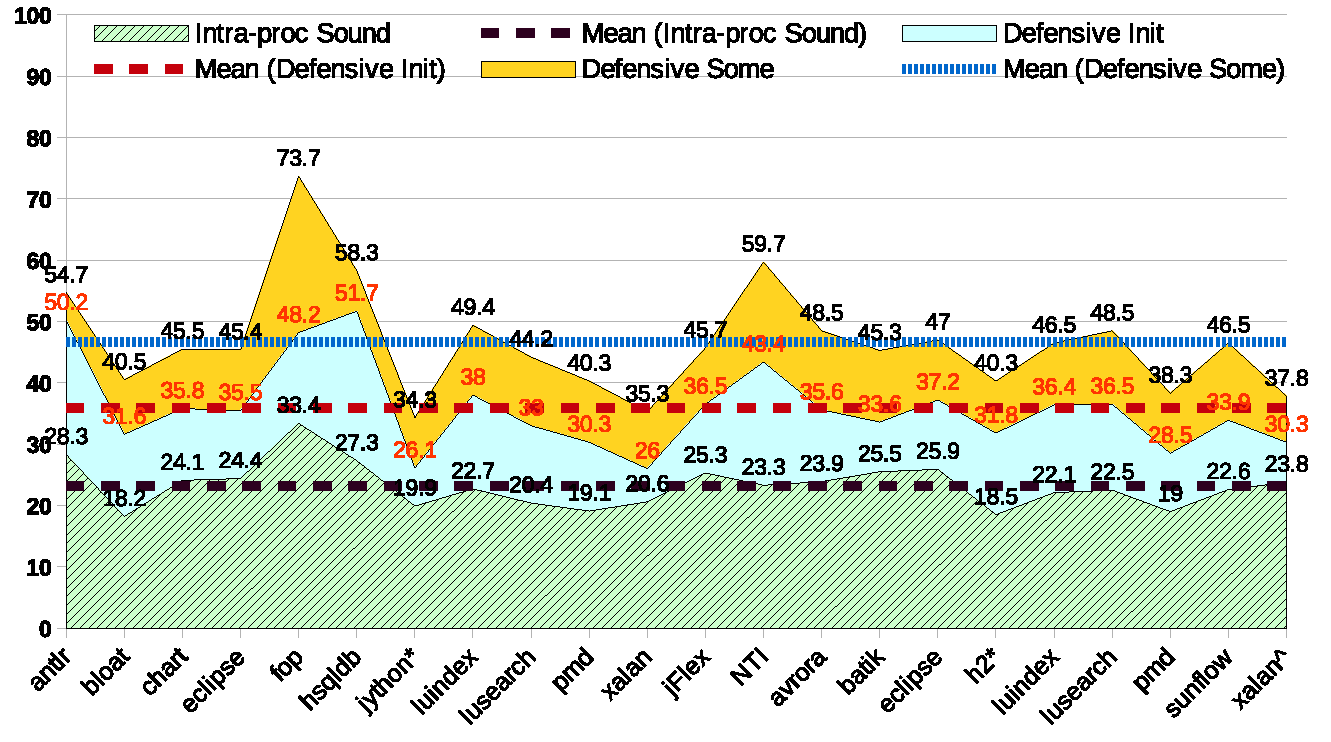
\includegraphics[width=\linewidth]{assets/defensive/vars.pdf}
\caption[Percentage of application variables that have non-empty points-to sets]{Percentage of application variables (deemed reachable by baseline 2objH analysis) that have non-empty points-to sets for defensive analysis under some context and \ctxInit{} context (no assumptions). Intra-procedural sound points-to analysis (defensive minus the complex cases) shown as baseline. Arithmetic means are plotted as lines.}
\label{fig:sound:coverage}
\end{figure}

Thus, the defensive analysis achieves a large proportion of the benefits of an unsound analysis, while guaranteeing these results against uses of opaque code. We can answer \textbf{RQ1} affirmatively: defensive analysis covers a large part of realistic programs (over one-third unconditionally; close to one half under specific calling conditions), despite its conservative nature.


\paragraphhead{Comparison with intra-procedural.}
We have earlier referred to the ``easy'', intra-procedural parts of the analysis reasoning: what a compiler or VM would likely do to perform sound local data-flow analysis. This is the subject of \textbf{RQ2}, also answered by Figure~\ref{fig:sound:coverage}. The figure includes results for an intra-procedural baseline analysis that captures the low-hanging fruit of sound reasoning: local variables that directly or transitively (via ``move'' instructions) get assigned an allocated object. That is, the ``Intra-proc Sound'' analysis is otherwise the same as the full ``defensive'' logic, with the exception of the new ``interesting'' cases (control-flow merging, heap manipulation, and inter-procedural propagation). 

The result answers \textbf{RQ2} affirmatively: defensive analysis has significantly higher coverage than the baseline intra-procedural analysis. (And the difference only grows when considering an actual client, in later experiments.) Although the benefit is not broken down further in the figure, the handling of method calls alone (i.e., rules \infer{Call}, \infer{Args} and \infer{Ret}) is responsible for the lion's share of the difference between the full defensive analysis and the intra-procedural sound analysis.


%%% SPACE
%% Two data points in the experiment require further explanation. The
%% hsqldb benchmark is analyzed only partially by the underlying 2objH
%% analysis with the given reflection settings. Less than 10\% of the
%% statically available application code is deemed reachable.
%% % by 2objH, and is consequently also analyzed by 5def. 
%% The comparison of 2objH and 5def in this subset is still
%% meaningful, but may not be representative of the full complexity.
%% % of the hsqldb code. 
%% Also, for jython, 5def seems to cover 34.5\% of the application
%% variables produced by 2objH. However, this number is likely biased
%% (lowered) by the \emph{imprecision} of the unsound analysis: jython is
%% analyzed with a context-insensitive analysis, resulting in many
%% variables with spurious points-to sets.
%% % (See also later metrics on precision for jython.)
%% %
%% %If we allowed the 2objH
%% %analysis to complete (beyond a 3hr timeout) the real coverage of 5def
%% %would likely be higher for this benchmark. 

\paragraphhead{Running time.} 
Figure~\ref{fig:sound:time} shows the running times of the analysis, plotted next to that of 2objH, for reference. Although the two analyses are dissimilar, 2objH is qualitatively the closest one can get to defensive analysis with the current state of the art: it is an analysis with high precision, run with best-effort soundness support. Therefore, 2objH can serve as a realistic point of reference. As can be seen, the running times of defensive analysis are realistically low, although its flow-sensitive and 5-call-site-sensitive nature suggests it would be a prohibitively heavy analysis. This answers \textbf{RQ3} and confirms the benefits of laziness: a defensive analysis that only populates points-to sets once they are definitely bounded, achieves scalability for deep context.

\begin{figure}[tbh]
\centering
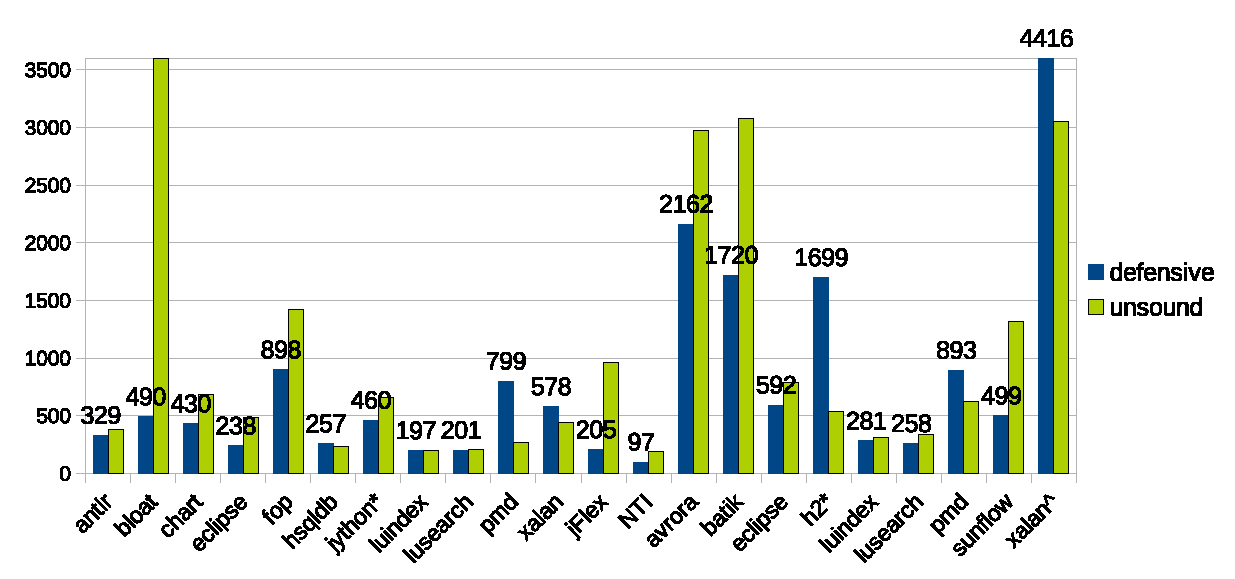
\includegraphics[width=\linewidth]{assets/defensive/time.pdf}
\caption[Execution time of defensive analysis vs. unsound baseline]{Execution time (in seconds) of defensive analysis, with running time of 2objH (with unsound reflection handling) shown as a baseline. Labels are shown for defensive analysis only to avoid crowding the plot.}
\label{fig:sound:time}
\end{figure}


\paragraphhead{Client analysis: devirtualization.}
Our baseline analysis, 2objH, is highly precise and effective in challenges such as devirtualizing calls (resolving virtual calls to a single target method). On average, it can devirtualize \nums{89.3\%} of the calls in the benchmarks studied (min \bad{78.5\%}, max \best{95.2\%}). However, these results are unsound and a compiler cannot act upon them. For optimization clients, such as devirtualization, soundness is essential. Using sound results, a JIT compiler can skip dynamic tests (of the inline caching optimization) for all calls that the analysis soundly covers.

Figure~\ref{fig:sound:devirt1} shows the virtual calls that defensive analysis devirtualizes, as a percentage of those devirtualized by the unsound analysis.

\begin{figure}[tbh]
\centering
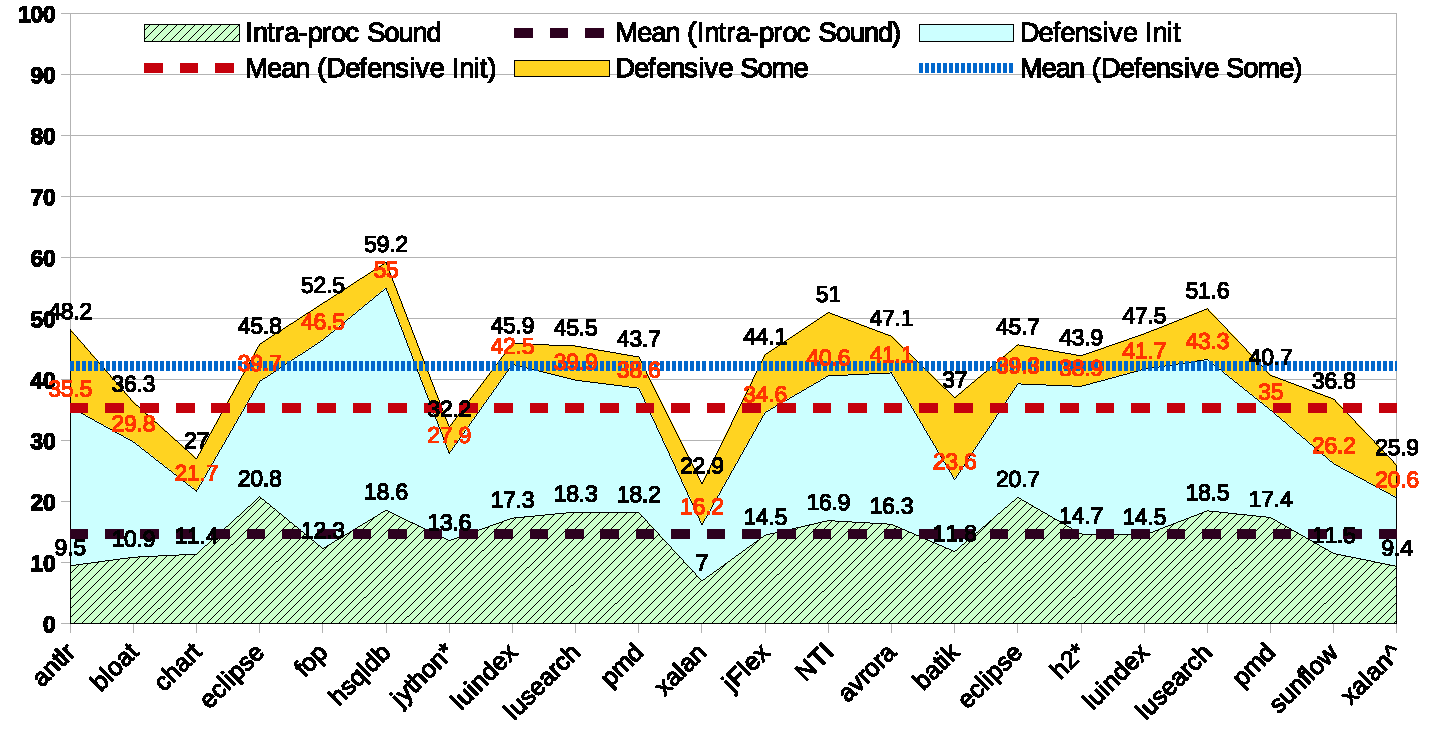
\includegraphics[width=\linewidth]{assets/defensive/devirt1.pdf}
\caption[Virtual call sites found with a single typed receiver objects]{Virtual call sites that are found to have receiver objects of a single type. These call sites can be soundly devirtualized. Numbers are shown as percentages of devirtualization achieved by unsound 2objH analysis.}
\label{fig:sound:devirt1}
\end{figure}

As can be seen, defensive analysis manages to recover a large part of the benefit of an unsound analysis (median \nums{44.8\%} for optimization under a context guard, \best{38.7\%} for unconditional, \ctxInit{} context, optimization), performing much better than the baseline intra-procedural must-analysis (at \bad{14.6\%}). This answers \textbf{RQ4} affirmatively: the coverage of defensive analysis translates into real benefit for realistic clients.


\paragraphhead{Concurrency model.}
A compiler (JIT or AOT) author may (rightly) remark that the concurrency model of Section~\ref{sec:sound:assumptions} is not appropriate for automatic optimizations. The Java concurrency model permits a lot more relaxed behaviors, so the analysis is not sound for full Java as stated. However, the benefit of defensive analysis is that it starts from a sound basis and can add to it conservatively, only when it is certain that soundness cannot possibly be violated. Accordingly, we can remove the assumption that all shared data are accessed while holding mutexes, by applying the load/store rules only when objects trivially do not escape their allocating thread. We show the updated numbers for the devirtualization client (now fully sound for Java!) in Figure~\ref{fig:sound:devirt2}. The difference in impact is minimal: \nums{43\%} of virtual call sites can be devirtualized conditionally, under some context, while \best{36\%} can be devirtualized unconditionally. This helps answer \textbf{RQ5}: defensive analysis can yield actionable results for a well-known optimization, under the Java memory model, for a large portion of realistic programs.

\begin{figure}[tbh]
\centering
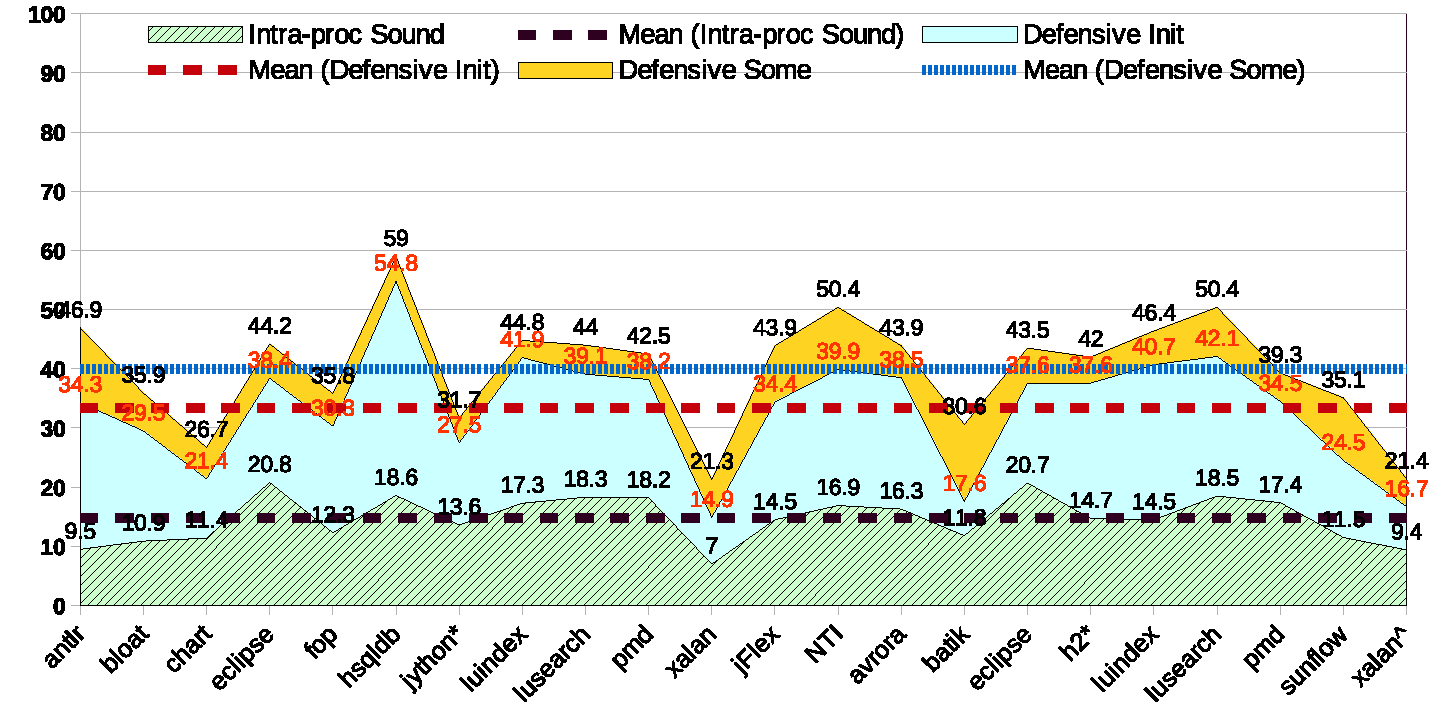
\includegraphics[width=\linewidth]{assets/defensive/devirt2.pdf}
\caption[Single typed, virtual call sites under a relaxed memory model]{Virtual call sites (percentage of 2objH) that are found to have receiver objects of a single type. Updates Figure~\ref{fig:sound:devirt1}, this time with soundness under a relaxed memory model.}
\label{fig:sound:devirt2}
\end{figure}


\paragraphhead{Points-to set sizes.}
Finally, it is interesting to quantify the precision of the defensive analysis, for the points-to sets it covers. This precision is expected to be high, since defensive analysis is flow- and context-sensitive, but exact figures help put it in perspective.

\begin{table*}[h!t]
\centering
\begin{tabular}{|c|l|cc!{\vrule width 2pt}cc|r|c|}
\cline{3-6}
\multicolumn{2}{c|}{} & defensive & 2objH & 2objH & defensive & \multicolumn{2}{c}{} \\
\cline{1-8}
\multirow{11}{0.4cm}{\rotatebox{90}{\mbox{DaCapo 2006-10-MR2}}}
& antlr     & 1.01  & 1.10  & 3.04  & 1.05  & avrora & \multirow{9}{0.4cm}{\rotatebox{90}{\mbox{DaCapo 9.12-Bach}}} \\
& bloat     & 1.02  & 2.12 	& 1.05  & 1.04  & batik & \\
& chart     & 1.09  & 1.09 	& 1.53  & 1.07  & eclipse & \\
& eclipse   & 1.06  & 1.31 	& 2.07  & 1.04  & h2* & \\
& fop       & 1.00  & 1.03 	& 1.04  & 1.01  & luindex & \\
& hsqld     & 1.01  & 1.04  & 1.08  & 1.03  & lusearch & \\
& jython*   & 1.01  & 6.05 	& 1.04  & 1.01  & pmd & \\
& luindex   & 1.02  & 1.02  & 1.08  & 1.05  & sunflow & \\
& lusearch  & 1.04  & 1.06 	& 1.19  & 1.04  & xalan\^ & \\
\cmidrule[2pt]{5-8}
& pmd       & 1.01  & 1.05 	& 1.02  & 1.01  & jFlex & \\
& xalan     & 1.05  & 1.12 	& 1.03  & 1.03  & NTI & \\
\cmidrule[2pt]{1-8}
\multicolumn{4}{|r|}{\textbf{``defensive'' mean}} & \multicolumn{4}{c|}{\best{1.03}} \\
\multicolumn{4}{|r|}{\textbf{``2objH'' mean}} & \multicolumn{4}{c|}{1.51} \\
\cline{1-8}
\end{tabular}
\caption[Avg. number of abstract objects pointed-by per variable]{Average number of abstract objects pointed-by per variable, for variables for which both analyses compute results.}
\label{tab:sound:precision}
\end{table*}

Table~\ref{tab:sound:precision} shows average points-to set sizes for the defensive analysis vs. the 2objH analysis. The sets (excluding null values) are computed over variables covered by both analyses, for non-empty defensive analysis sets and under context \ctxInit{} of the defensive analysis, i.e., unconditionally. (The numbers are for the simplistic concurrency model, but remain unchanged to two significant digits for the relaxed concurrency model.)

As can be seen, the defensive analysis is highly precise when it produces non-empty points-to sets, typically yielding points-to set sizes very close to 1. 2objH is also a very precise analysis (for variables with bounded points-to sets), so it remains competitive, yet clearly less precise. Notably, points-to set sizes close to 1 are the Holy Grail of points-to analysis: such precision is actionable for nearly all conceivable clients of a points-to analysis.


\section{Summary}

Static analysis has long suffered from unsoundness for perfectly realistic language features, such as reflection, native code, or dynamic loading. We presented a new analysis architecture that achieves soundness by being \emph{defensive}. Despite its conservative nature, the analysis manages to yield useful results for a large subset of the code in realistic Java programs, while being efficient and scalable. Additionally, the analysis is modular, as it can be applied to any subset of a program and will yield sound results.

We expect this approach to open significant avenues for further work. The analysis architecture can serve as the basis of other sound analysis designs. The defensive analysis itself can be combined with several other analyses (may-escape, must-alias) that have so far been hindered by the lack of a sound substrate.

\part{Epilogue}
%\chapter{paNda: a Datalog compiler}\label{chapter:panda}

\epigraph{Always take a banana to a party.}{\textit{The 10th Doctor} - Doctor Who}
%\chapter{Related Work}\label{chapter:related}

\section{Hybrid}

We have discussed directly related work throughout the paper. Here we
selectively mention a few techniques that, although not directly
related to ours, offer alternative approaches to sweet spots in the
precision/performance tradeoff.

Special-purpose combinations of context-sensitivity have been used in
the past, but have required manual identification of classes to be
treated separately (e.g., Java collection classes, or library factory
methods). An excellent representative is the TAJ work for taint
analysis of Java web applications
\cite{pldi:2009:Tripp}. In contrast, we have sought to
map the space and identify interesting hybrids for general application
of context-sensitivity, over the entire program.

The analyses we examined are context-sensitive but flow-insensitive.
We can achieve several of the benefits of flow-sensitivity by applying
the analysis on the static single assignment (SSA) intermediate form
of the program. This is easy to do with a mere flag setting on the
\doop{} framework. However, the impact of the SSA transformation
on the input is minimal. The default intermediate language used as
input in \doop{} (the Jimple representation of the Soot
framework \cite{cascon:1999:Vall,cc:2000:Vall}) is already close to
SSA form, although it does not guarantee that every variable is
strictly single-assignment without requesting it explicitly.  Recent
work by Lhot\'{a}k and Chung \cite{popl:2011:Lhotak} has shown that
much of the benefit of flow-sensitivity derives from the ability to do
strong updates of the points-to information. Lhot\'{a}k and Chung then
exploited this insight to derive analyses with similar benefit to a
full flow-sensitive analysis at lower cost.

A demand-driven evaluation strategy reduces the cost of an analysis by
computing only those results that are necessary for a client program
analysis~\cite{oopsla:2005:Sridharan,pldi:2006:Sridharan,popl:2008:Zheng,pldi:2001:Heintze}. This is a useful
approach for client analyses that focus on specific locations in a
program, but if the client needs results from the entire program, then
demand-driven analysis is typically slower than an exhaustive
analysis.

Reps~\cite{cc:1994:Reps} showed how to use the standard magic-sets
optimization to automatically derive a demand-driven analysis
from an exhaustive analysis (like ours). This optimization
combines the benefits of top-down and bottom-up evaluation of
logic programs by adding side-conditions to rules that limit
the computation to just the required data.

An interesting recent approach to demand-driven analyses was
introduced by Liang and Naik \cite{pldi:2011:Liang}.
Their ``pruning'' approach consists of first computing a coarse
over-approximation of the points-to information, while keeping the
provenance of this derivation, i.e., recording which input facts have
affected each part of the output. The input program is then pruned so
that parts that did not affect the interesting points of the output
are eliminated. Then a precise analysis is run, in order to establish
the desired property.


\section{Introspective}

The effort to tune the context-sensitivity of an analysis is pervasive
in the literature. Nevertheless, most approaches fundamentally differ
from ours, either by trying to vary context-sensitivity based on
syntactic properties or by trying to focus on only a part of the program
that matters for answering a given query.
In contrast, we attack the context-sensitive scalability problem 
head-on, in the all-points points-to analysis setting, with context
used all over the program and library.

Typical scalable points-to analysis frameworks such as
Wala~\cite{www:wala} and Doop~\cite{oopsla:2009:Bravenboer} employ a multitude of
low-level heuristics for tuning the precision and scalability of an
analysis. These include using extra context for collection classes,
using a heap context for arrays in an analysis without a
context-sensitive heap, allocating strings or exceptions
context-insensitively, treating library factory methods with deeper
context, etc. Such heuristics are typically user-selected and
prominent in the documentation of the respective frameworks, and have
also appeared in the literature (e.g.,
\cite{pldi:2009:Tripp,cc:2013:Kastrinis}).  However, all
such approaches are mere hard-wired heuristics and do not address the
major scalability problem that our approach aims to solve. The
scalability issues identified in earlier literature and discussed
throughout this paper are present after all such heuristics have been
employed.
% These
%heuristics are already implemented in the baseline framework that we
%use for our analysis. 

A more general approach is \emph{hybrid} context-sensitivity, which
consists of treating virtual and static method calls differently
\cite{pldi:2013:Kastrinis}. Such a hybrid analysis attempts to emulate
call-site sensitivity for static method calls and object-sensitivity
for dynamic calls. The approach becomes interesting when context is
deep (e.g., how are context elements merged when a dynamic call is
made inside a static call?). Nevertheless, the hybrid
context-sensitivity approach does not change the essence of the
problem we are trying to solve. For hard-to-analyze applications,
hybrid context-sensitive algorithms are equally unscalable as their
component algorithms. For the purposes of our experimental study,
which only tests the scalability of heavyweight benchmarks, hybrid
context-sensitivity is virtually indistinguishable from object-
sensitivity.

More interesting applications of selective context-sensitivity have
been explored in the context of \emph{demand-driven} pointer analysis.
A demand-driven evaluation strategy reduces the cost of an analysis by
computing only those results that are necessary for a client program
analysis~\cite{oopsla:2005:Sridharan,pldi:2006:Sridharan,popl:2008:Zheng,pldi:2001:Heintze}. This is a useful
approach for client analyses that focus on specific locations in a
program, but if the client needs results from the entire program, then
demand-driven analysis is typically slower than an exhaustive
analysis.

In the demand-driven space, refinement-based analyses have been used
primarily in the work of Sridharan and Bod\'{\i}k~\cite{pldi:2006:Sridharan} and
of Liang and Naik~\cite{pldi:2011:Liang}.  Sridharan
and Bod\'{\i}k~\cite{pldi:2006:Sridharan} introduce refinement-based analysis as a
way to adaptively increase the precision characteristics of an
existing analysis algorithm when a client analysis is not satisfied
with the result. The approach allows turning on field-sensitivity, as
well as higher call-site sensitivity for an analysis algorithm. Yet,
unlike ours, it is not a general approach that can apply to any kind
of context and a large number of different algorithms.  Liang and
Naik's ``pruning'' approach \cite{pldi:2011:Liang}
consists of first computing a coarse over-approximation of the
points-to information, while keeping the provenance of this
derivation, i.e., recording which input facts have affected each part
of the output. The input program is then pruned so that parts that did
not affect the interesting points of the output are eliminated. Then a
highly context-sensitive precise analysis is run, in order to
establish the desired property. This approach is similar to
introspective context-sensitivity in that the analysis is run twice
and a separate query over the first-run result determines the second
run's characteristics.  Nevertheless, our approach requires no
provenance computation (which is unlikely to scale for an all-points
analysis) and works even when we want answers for the entire
program---i.e., when pruning is not possible.

Both of the above demand-driven approaches can be viewed as
complements of our introspective context-sensitivity. In the
demand-driven world, it is possible to estimate the \emph{benefit}
that a more precise analysis may yield: either the client is happy
with the current level of precision (which implies there is no further
benefit to be obtained) or it is not, in which case more precision
should be added. In our all-points pointer analysis problem we have no
such information. This motivates our \emph{cost}-based heuristics,
which attempt to estimate ``what can go wrong'' when more precision
gets added, as opposed to ``what can be gained'', as in demand-driven
techniques.


\section{Must-Analysis: Logic}

There are several approaches in the literature that present
must-analyses in the pointer analysis setting or employ them in a
may-analysis. Our approach is a must-alias analysis applied to Java
bytecode, but conceptually it is distinguished by its minimizing the
distance between the implementation and the declarative specification.
%% and by its leveraging of a highly-efficient data structure for sets of
%% alias classes.

%% Ma et al.~\cite{isola:2008:Ma} present an algorithm for
%% null-pointer dereference detection using a
%% context-insensitive may-alias and a must-alias analysis; the latter is
%% used to increase the precision of the former, by enabling strong
%% updates when possible.

Nikoli\'{c} and Spoto~\cite{ictac:2012:Nikolic} present a
must-alias analysis that tracks aliases between program expressions
and local variables (or stack locations, since they analyze Java
bytecode%% , which is a stack-based representation
).  The analysis
%itself does not expose any clear configuration points but it 
is related to ours both because of its application to Java bytecode
and because it is constraint-based: the analysis is a generator of
constraints, which are subsequently solved to produce the analysis
results.
% Abstractly,
%this is a relative of our Datalog-based approach, but it is unclear
%how the two may compare in terms of engineering tradeoffs.

Hind et al. \cite{article:1999:Hind} present a collection of pointer
analysis algorithms. Among them, the most relevant to this work is a
flow-sensitive interprocedural pointer alias analysis. The authors
optimistically produce \emph{must} information for pointers to single
non-summary objects.

Emami et al.~\cite{pldi:1994:Emami} present an approach that
simultaneously calculates both must- and may-point-to information for
a C analysis. Their empirical results ``show the existence of a
substantial number of definite points-to relationships, which forms
very valuable information''---much in line with our own
experience.

Must- information is often computed in conjunction with a
client analysis. One of the best examples is the typestate
verification of Fink et al.~\cite{issta:2006:Fink}, which demonstrates the value of
a must-analysis and the techniques that enable it.

The analysis of \cite{ecoop:2012:De} is essentially a
flow-sensitive may-point-to analysis that performs strong updates, as
it maps \emph{access paths} to \emph{heap objects} (abstracted by
their allocation sites). 
The approach uses a flow-insensitive
may-point-to analysis to bootstrap the main analysis. However, it
provides no \emph{definite} knowledge of any sort, since the aim is to
increase the precision of the may-analysis. For instance, even if an
access path points to a single heap object, according to the De and
D'Souza analysis, there is no \emph{must} point-to information
derived, since this object could be a summary object (i.e., one that
abstracts many objects allocated at the same allocation site). To
reason about such cases, other approaches, such as the more expensive
shape analysis algorithms \cite{article:2002:Sagiv},
additionally maintain summary information per heap object. In this
way, they allow must point-to edges to exist only if the target is
definitely not a summary node.

%An alternative approach to handle this shortcoming is to propagate
%% An approach for integrating \emph{must} point-to reasoning in an
%% analysis is to propagate such
%% %\emph{must}-point-to 
%% information only at instructions where we know that the given heap
%% allocation target still refers to the last object allocated at that
%% site \cite{Altucher:1995:EFM:199448.199466}. Thus, an execution path
%% that may create another object at the same site (such as when reaching
%% the end of the loop) would invalidate any previous must-point-to facts
%% (i.e., it will stop them from propagating any further).

Generally, must-analyses can vary greatly in sophistication and can be
employed in an array of different combinations with may-analyses.  The
analysis of Balakrishnan and Reps~\cite{sas:2006:Balakrishnan}, which
introduces the \emph{recency abstraction}, distinguishes between the
most recently allocated object at an allocation site (a concrete
object, allowing strong updates) and earlier-allocated objects
(represented as a summary node). The analysis additionally keeps
information on the size of the set of objects represented by a summary
node. At the extreme, one can find full-blown shape analysis
approaches, such as that of Sagiv et
al.~\cite{article:2002:Sagiv}, which explicitly maintains must-
and may- information simultaneously, by means of three-valued truth
values, in full detail up to predicate abstraction: a
relationship can definitely hold (``must''), definitely not hold
(``must not'', i.e., negation of ``may''), or possibly hold
(``may''). Summary and concrete nodes are again used to represent
knowledge, albeit in full detail, as captured by arbitrary predicates
whose value is maintained across program statements, at the cost of a
super-exponential worst-case complexity.

%% Jagannathan et al.~\cite{popl:1998:Jagannathan} present
%% an algorithm for must-alias analysis of functional languages. The
%% algorithm adapts must-alias insights to the setting of captured
%% variables.
%% %captured in closures.  
%% For instance, must-alias information for
%% non-summary objects permits strong updates, which the authors find to
%% improve analysis precision. We employ must-alias analysis results
%% quite similarly in applications of our model analysis.


%% Our optimized data structure is (partly) based on the observation that
%% must-alias sets are equivalence classes. This is not the first time
%% that a data structure that efficiently implements equivalence classes
%% has been used to speed up pointer analysis. Most notably, a
%% Steensgaard-style (or \emph{unification-based})
%% \cite{steensgard:1996:PointsTo} analysis computes may-point-to sets
%% that are equivalence classes. This means that points-to sets are
%% disjoint---if two points-to sets are found to possibly overlap, they
%% get unified. This loses precision (relative to a standard subset-based
%% points-to analysis) but enables the algorithm to use union-find trees
%% for a very efficient representation.

%% Another optimized data structure often used in pointer analysis is the
%% \emph{constraint graph}: a graph with nodes denoting pointer variables
%% and an edge between nodes \code{p} and \code{q} denoting flow (e.g., a
%% direct assignment) from variable \code{p} to variable \code{q}.  Online
%% cycle elimination by F\"{a}ndrich et al.
%% \cite{pldi/FahndrichFSA98} detects cycles in the
%% constraint graph and collapses all nodes in a cycle into a
%% representative node, since such nodes will have identical points-to
%% information. The technique of Nasre
%% \cite{ismm/Nasre12} extends such constraint graph
%% reasoning based on the observation that if two nodes have the same
%% dominator in the constraint graph, then they are clones: the values
%% flowing to them are (only) those of the dominator node. Several other
%% constraint graph optimizations are applied off-line (i.e., before the
%% points-to analysis runs).  Prime examples of such techniques are
%% Rountev and Chandra's \cite{rountevOffline} and Hardekopf and Lin's
%% \cite{hardekopfOffline}. (Hardekopf and Lin have also applied similar
%% ideas in a hybrid online/offline setting \cite{antgrasshopper}.)  Both
%% of these techniques perform an off-line detection of equivalent
%% points-to sets and use this knowledge to eliminate redundant work in
%% subsequent points-to computations. Our data structure can be seen as
%% somewhat analogous to constraint-graph techniques, in the sense that
%% we do not compute the flow of objects or the fully expanded set of all
%% possible alias pairs. Instead, we compute the ``wiring'' (i.e., the
%% alias relationships, locally, that the program induces) and keep the
%% alias information in condensed form, until it needs to be queried by a
%% client analysis.

%% %Hardekopf and
%% %Lin's approach is impressively general, computing hash codes that
%% %encode all the logical processing of a points-to set that is induced
%% %by the current program and, thus, detecting equivalent points-to sets
%% %even through complex program patterns.

%% % \citep{Heintze:2001:UAA:378795.378855} ; pre-transitive constraint-graph and reachability caching


\section{Must-Analysis: Datastructure}

There are several approaches in the literature that present
must-analyses in the pointer analysis setting or employ them in a
may-analysis. Additionally, there are several approaches that
integrate efficient data structures in the representation of
points-to information.


\paragraph{Data Structures and Heap Abstractions.}
Our optimized data structure is (partly) based on the observation that
must-alias sets are equivalence classes. This is not the first time
that a data structure that efficiently implements equivalence classes
has been used to speed up pointer analysis. Most notably, a
Steensgaard-style (or \emph{unification-based})
\cite{popl:1996:Steensgaard} analysis computes may-point-to sets
that are equivalence classes. This means that points-to sets are
disjoint---if two points-to sets are found to possibly overlap, they
get unified. This loses precision (relative to a standard subset-based
points-to analysis) but enables the algorithm to use union-find trees
for a very efficient representation.

Another optimized data structure often used in pointer analysis is the
\emph{constraint graph}: a graph with nodes denoting pointer variables
and an edge between nodes \code{p} and \code{q} denoting flow (e.g., a
direct assignment) from variable \code{p} to variable \code{q}.  Online
cycle elimination by F\"{a}ndrich et al.
\cite{pldi:1998:Fahndrich} detects cycles in the
constraint graph and collapses all nodes in a cycle into a
representative node, since such nodes will have identical points-to
information. The technique of Nasre
\cite{ismm:2012:Nasre} extends such constraint graph
reasoning based on the observation that if two nodes have the same
dominator in the constraint graph, then they are clones: the values
flowing to them are (only) those of the dominator node. Several other
constraint graph optimizations are applied off-line (i.e., before the
points-to analysis runs).  Prime examples of such techniques are
Rountev and Chandra's \cite{pldi:2000:Rountev} and Hardekopf and Lin's
\cite{sas:2007:Hardekopf}. (Hardekopf and Lin have also applied similar
ideas in a hybrid online/offline setting \cite{pldi:2007:Hardekopf}.)  Both
of these techniques perform an off-line detection of equivalent
points-to sets and use this knowledge to eliminate redundant work in
subsequent points-to computations. Our data structure can be seen as
somewhat analogous to constraint-graph techniques, in the sense that
we do not compute the flow of objects or the fully expanded set of all
possible alias pairs. Instead, we compute the ``wiring'' (i.e., the
alias relationships, locally, that the program induces) and keep the
alias information in condensed form, until it needs to be queried by a
client analysis.

Another conceptual relative of our data structure is the model
presented by Madhavan et al. \cite{article:2015:Madhavan} for modular \emph{may}
analyses. That model is similar in that it invents abstract nodes for
heap objects that resemble ours (without the equivalence-class
nature). The Madhavan et al. approach aims to achieve modular
reasoning, i.e., to model the heap effects of a method without knowing
its calling environment. To do so, the approach creates abstract
nodes that represent concepts such as ``whichever object variable
\code{x} may point to''. Our data structure has nodes with a similar
meaning, however we also take advantage of the ``must'' nature of
the analysis to merge nodes, every time the same access path can
reach both.


\paragraph{Must-Analyses for Aliasing.}
There are several instances of past work that apply must reasoning in
pointer analysis. These mostly serve to paint the landscape of
potential applicability of our data structure.

Ma et al.~\cite{isola:2008:Ma} present an algorithm for
null-pointer dereference detection using a context-insensitive
may-alias and a must-alias analysis; the latter is used to increase
the precision of the former, by enabling strong updates when possible.

Nikoli\'{c} and Spoto~\cite{ictac:2012:Nikolic} present a
must-alias analysis that tracks aliases between program expressions
and local variables (or stack locations, since they analyze Java
bytecode, which is a stack-based representation).  The analysis is a
generator of constraints, which are subsequently solved to produce the
analysis results.
% Abstractly,
%this is a relative of our Datalog-based approach, but it is unclear
%how the two may compare in terms of engineering tradeoffs.

Hind et al. \cite{article:1999:Hind} present a collection of pointer
analysis algorithms. Among them, the most relevant to this work is a
flow-sensitive interprocedural pointer alias analysis. The authors
optimistically produce \emph{must} information for pointers to single
non-summary objects.

Emami et al.~\cite{pldi:1994:Emami} present an approach that
simultaneously calculates both must- and may-point-to information for
a C analysis. Their empirical results ``show the existence of a
substantial number of definite points-to relationships, which forms
very valuable information''---much in line with our own
experience.

Must- information is often computed in conjunction with a
client analysis. One of the best examples is the typestate
verification of Fink et al.~\cite{issta:2006:Fink}, which demonstrates the value of
a must-analysis and the techniques that enable it.

%% The analysis of \cite{ecoop:2012:De} is essentially a
%% flow-sensitive may-point-to analysis that performs strong updates, as
%% it maps \emph{access paths} to \emph{heap objects} (abstracted by
%% their allocation sites). 
%% The approach uses a flow-insensitive
%% may-point-to analysis to bootstrap the main analysis. However, it
%% provides no \emph{definite} knowledge of any sort, since the aim is to
%% increase the precision of the may-analysis. For instance, even if an
%% access path points to a single heap object, according to the De and
%% D'Souza analysis, there is no \emph{must} point-to information
%% derived, since this object could be a summary object (i.e., one that
%% abstracts many objects allocated at the same allocation site). To
%% reason about such cases, other approaches, such as the more expensive
%% shape analysis algorithms \cite{article:2002:Sagiv},
%% additionally maintain summary information per heap object. In this
%% way, they allow must point-to edges to exist only if the target is
%% definitely not a summary node.

%An alternative approach to handle this shortcoming is to propagate
An approach for integrating \emph{must} point-to reasoning in an
analysis is to propagate such
%\emph{must}-point-to 
information only at instructions where we know that the given heap
allocation target still refers to the last object allocated at that
site \cite{popl:1995:Altucher}. Thus, an execution path
that may create another object at the same site (such as when reaching
the end of the loop) would invalidate any previous must-point-to facts
(i.e., it will stop them from propagating any further).

Generally, must-analyses can vary greatly in sophistication and can be
employed in an array of different combinations with may-analyses.  The
analysis of Balakrishnan and Reps~\cite{sas:2006:Balakrishnan}, which
introduces the \emph{recency abstraction}, distinguishes between the
most recently allocated object at an allocation site (a concrete
object, allowing strong updates) and earlier-allocated objects
(represented as a summary node). The analysis additionally keeps
information on the size of the set of objects represented by a summary
node. At the extreme, one can find full-blown shape analysis
approaches, such as that of Sagiv et
al.~\cite{article:2002:Sagiv}, which explicitly maintains must-
and may- information simultaneously, by means of three-valued truth
values, in full detail up to predicate abstraction: a
relationship can definitely hold (``must''), definitely not hold
(``must not'', i.e., negation of ``may''), or possibly hold
(``may''). Summary and concrete nodes are again used to represent
knowledge, albeit in full detail, as captured by arbitrary predicates
whose value is maintained across program statements, at the cost of a
super-exponential worst-case complexity.

Jagannathan et al.~\cite{popl:1998:Jagannathan} present
an algorithm for must-alias analysis of functional languages. The
algorithm adapts must-alias insights to the setting of captured
variables.
%captured in closures.  
For instance, must-alias information for
non-summary objects permits strong updates, which the authors find to
improve analysis precision. We employ must-alias analysis results
quite similarly in applications of our model analysis.



%Hardekopf and
%Lin's approach is impressively general, computing hash codes that
%encode all the logical processing of a points-to set that is induced
%by the current program and, thus, detecting equivalent points-to sets
%even through complex program patterns.

% \citep{Heintze:2001:UAA:378795.378855} ; pre-transitive constraint-graph and reachability caching


\section{Defensive Analysis}

There is certainly past work that attempt to ensure a sound
whole-program analysis, but none matches the generality and
applicability of our approach. We selectively discuss representative
approaches.

The standard past approach to soundness for a careful static analysis
has been to ``bail out'': the analysis detects whether there are
program features that it does not handle soundly, and issues warnings,
or refuses to produce answers. This is a common pattern in
abstract-interpretation~\cite{popl:1977:Cousot} analyses,
such as Astr\'{e}e~\cite{sas:2007:Delmas}, which have traditionally
emphasized sound handling of conventional language features. However,
this is far from a solution to the problem of being sound for opaque
code: refusing to handle the vast majority of realistic programs can
be argued to be sound, but is not usefully so. In contrast, our work
handles \emph{all} realistic programs, but returns partial (but sound)
results, i.e., produces non-empty points-to sets for a subset of the
variables. It is an experimental question to determine whether
this subset is usefully large, as we do in our evaluation.

%\citet{ecoop:2004:Hirzel,article:2007:Hirzel}
Hirzel et al. \cite{ecoop:2004:Hirzel,article:2007:Hirzel} use an
online pointer analysis to deal with reflection and dynamic loading by
monitoring their run-time occurrence, recording their results, and
running the analysis again, incrementally. However, this is hardly a
\emph{static} analysis and its cost is prohibitive for precise
(context-sensitive) analyses, if applied to all reflection
actions. 

%\citet{pldi:2007:Lattner}
Lattner et al. \cite{pldi:2007:Lattner} offer an algorithm that can apply to incomplete
programs, but it assumes that the linker can know all callers (i.e.,
there is no reflection---the analysis is for C/C++) and the approach
is closely tied to a specific flow-insensitive, unification-based
analysis logic~\cite{popl:1996:Steensgaard}, necessary
for simultaneously computing inter-related points-to, may-alias, and
may-escape information.

%\citet{pldi:2000:Sreedhar}
Sreedhar et al. \cite{pldi:2000:Sreedhar} present the
only past approach to explicitly target dynamic class loading,
although only for a specific client analysis (call
specialization). Still, that work ends up making many statically
unsound assumptions (requiring, at the very least, programmer
intervention), illustrating well the difficulty of the problem, if not
addressed defensively. The approach assumes that only the public API
of a ``closed world'' is callable, thus ignoring many uses of
reflection. (With reflection, any method is callable from unknown
code, and any field is accessible.) It ``[does] not address the Java
features of reloading and the Java Native Interface''. It
``optimistically assumes'' that ``[the extant state of statically
  known objects] remains unchanged when they become reachable from
static reference variables''. It is not clear whether the technique is
conservative relative to adversarial native code (in system libraries,
since the JNI is ignored). Finally, the approach assumes the existence
of a sound may-point-to analysis, even though none exists in practice!
% (i.e., the points-to analysis may miss
%objects when asked ``what objects can this variable point to'', as it is
%in the Sreedhar et al. paper).

Traditional conservative call-graph construction (\emph{Class
  Hierarchy Analysis (CHA)} \cite{ecoop:1995:Dean} or
\emph{Rapid Type Analysis (RTA)} \cite{oopsla:1996:Bacon}) is
unsound.  Such algorithms explore the entire class hierarchy for
matching (overriding) methods and consider all of them to be potential
virtual call targets. However, even this is not sufficient for a sound static
analysis of opaque code: classes can be generated and loaded
dynamically during program execution. CHA cannot find target methods
that do not even exist statically, yet modeling them is precisely what
is needed for soundness in real-world conditions. For instance, Java
applications, especially in the enterprise (server-side) space, employ
dynamic loading heavily, and patterns such as \emph{dynamic proxies}
have been standardized and used widely since the early Java days.

Furthermore, such heuristic ``best-effort'' over-approximation is
detrimental to analysis precision and performance. CHA is an example
of a loose over-approximation in an effort to capture most dynamic
behaviors.
%(Similar loose over-approximations have been proposed, for
%instance, for reflection analysis~\cite{aplas:2015:Smaragdakis}.) 
Loose over-approximations compute many more possible targets than
those that realistically arise. This yields vast points-to sets that
render the analysis heavyweight and useless due to imprecision.
(Avoiding such costs is exactly why past analyses have often opted for glaringly
unsound handling of opaque code features.)
Our lazy representation of ``don't know''/''cannot bound'' values as empty
sets addresses the problem, by keeping all points-to sets compact.


The conventional handling of reflection in may-point-to analysis
algorithms for
Java~\cite{www:wala-reflection,ecoop:2014:Li,aplas:2005:Livshits,thesis:Livshits,aplas:2015:Smaragdakis,sas:2015:Li}
is unsound, instead relying on a ``best-effort'' approach.  Such past
analyses attempt to statically model the result of reflection
operations, e.g., by computing a superset of the strings that can be
used as arguments to a \code{Class.forName} operation (which accepts a
name string and returns a reflection object representing the class
with that name).
The analyses are unsound when faced with a completely unknown string:
instead of assuming that \emph{any} class object can be returned, the
analysis assumes that \emph{none} can. The reason is that
over-approximation (assuming any object is returned) would be
detrimental to the analysis performance and precision. Even with an
unsound approach, current algorithms are heavily burdened by the use
of reflection analysis. For instance, the documentation of the
\textsc{Wala} library directly blames reflection analysis for
scalability shortcomings
\cite{www:wala-reflection},\footnote{The \textsc{Wala} documentation
  is explicit: ``\emph{Reflection usage and the
    size of modern libraries/frameworks make it very difficult to
    scale flow-insensitive points-to analysis to modern Java
    programs. For example, with default settings, WALA's pointer
    analyses cannot handle any program linked against the Java 6
    standard libraries, due to extensive reflection in the
    libraries.}''~\cite{www:wala-reflection}} and enabling reflection
on the \textsc{Doop} framework slows it down by an order of magnitude
on standard benchmarks~\cite{aplas:2015:Smaragdakis}.
% SPACE
Furthermore, none
of these approaches attempt to model dynamic loading---a ubiquitous
feature in Java enterprise applications.

%Most importantly,
%however, no such approach can possibly ever be sound purely
%statically. Even if the analysis could feasibly assume that \emph{any}
%class object is returned by a \code{forName} operation, this
%%over-approximation 
%cannot account for dynamically generated and loaded
%classes---a ubiquitous feature in Java enterprise
%applications.%
%\chapter{Conclusions and Future Work}
\label{chapter:conclusions}
\epigraph{Everything’s got to end sometime. Otherwise nothing would ever get started.}{\textit{The 11th Doctor} - Doctor Who}

In this final chapter, we assess our initial thesis and conclude, while also considering interesting directions for future work.

The first part of our dissertation thesis states that it is possible to obtain \emph{precise} yet \emph{scalable} static pointer analysis algorithms by carefully employing different policies for different parts of the program.

In Chapter~\ref{chapter:hybrid}, we presented an analysis that combines call-site sensitivity and object sensitivity in a non-trivial manner. Instead of keeping both context flavors at all times, we alter an object-sensitive analysis so that it uses call-site sensitive elements in places where it would be more beneficial (e.g., in handling static call invocations). We show that this approach not only bears the precision benefits of combining the two flavors, but also avoids incurring the accumulated cost. For instance, in our experiments we observed an average speedup of \best{1.53x} alongside a more precise analysis. Additionally, we provide a concise way to formulate variations of both a uniform and a selective approach, in order to experiment with different flavor combinations and context depths.

In Chapter~\ref{chapter:introspective}, \emph{introspective analysis} examines another approach to a precise and scalable analysis. Our two-phase algorithm allows for a cheap, yet imprecise, analysis to run as a first step in order to gather crucial metrics that gauge the potential effect that a more precise context might have on various program elements (e.g., object allocations or method invocations). Subsequently, a more precise analysis is applied only on those elements that were deemed to benefit from the additional precision, without at the same time imposing a significant penalty on performance.

We employ various heuristics for deciding which program elements are worth the extra effort of a more precise handling, and show experimentally that although it is not a ``first line of defense'' kind of analysis, introspective analysis can be a valuable ``if all else fails'' alternative. Users can ``dial-in'' scalability (by parametrizing the heuristics that decide which elements are to be handled more accurately) to the exact level required, without having to sacrifice a significant fraction of precision. Previously hopeless analyses now become feasible. For instance, a variation of our analysis scales to all but one benchmark in under \best{20 minutes}, while keeping about \nums{2/3} of the precision gains that a more precise, yet ``heavy'' analysis would achieve.

The second part of our thesis stipulates that analyses can be designed to offer novel, strong guarantees on the soundness of results, but only for specific parts of the program.

In Chapters~\ref{chapter:must-logic} and \ref{chapter:must-data}, we model an instance of a \emph{must}-alias analysis, a conservative analysis that \emph{under}-approximates results but can guarantee that what is reported is actually correct. The nature of the analysis makes it valuable for compiler optimizations, program understanding, the improvement of bug detectors, and even as an internal component in more sophisticated analyses.

The analysis we present is minimal, yet it models core features in a handful of declarative rules. This makes reasoning about the analysis semantics less arduous. For instance, this partially led to the insights that called for the introduction of a specialized data structure in Chapter~\ref{chapter:must-data}. Additionally, the analysis highlights a non-conventional use of context; instead of a beneficial add-on, it is a crucial part of the analysis that guarantees that interprocedural propagation of information remains valid. Another benefit stemming from our analysis is its \emph{incrementality}. Soundness is not compromised if only a portion of the program-under-analysis or its libraries are available; only completeness. The availability of more code simply implies more inferences for our analysis. Precomputed facts are guaranteed to always hold, independently of what new parts of the code are analyzed in the future.

Following our insights from Chapter~\ref{chapter:must-logic}, we introduce a specialized data structure that exploits the fact that must-alias sets are equivalence classes, and as such there is no need to explicitly compute each alias pair. This ``laziness'' in computation is further exploited to implicitly encode the extension of alias information to longer access paths. Our data structure is in the form of a alias graph that abstractly represents local variables and the heap. Nodes (abstract objects) are alias classes, edges are field-points-to relationships.

In a complementary fashion, we describe all the algorithms on our alias graph required by a must-alias analysis. We implemented our data structure both imperatively, in Java, with destructive updates, and purely functionally, in Datalog. Both implementations yield large performance improvements compared to an explicit representation of all alias pairs. The imperative version achieves a speedup of up to \best{two orders} of magnitude, with the declarative implementation nearly matching it in most cases. As a result, the running time of a realistic must-alias analysis becomes small---\best{a few tens of seconds} for large benchmarks and the full Java library.

Finally, in Chapter~\ref{chapter:defensive}, we conclude our contributions with another conservative and \emph{fully sound} may-analysis. Soundness in our \emph{defensive analysis} means that it has to (correctly) over-approximate all concrete executions. This proves quite challenging in practice due to code that cannot be analyzed (e.g., dynamically generated code, or native code) or dynamic language features (e.g., reflection).

The analysis employs a different logical approach from past analyses, in order to successfully distinguish ``safe'' inferences (i.e., certain to not be affected by unknown code, and hence correct).  In essence, our analysis produces inferences only when these are guaranteed to hold because of existing code, and cannot possibly be violated by other, unknown code. In our effort to implement defensive analysis in a realistic package, we found that \emph{laziness} is an essential feature---the analysis cannot scale without it for real-world programs.

Experiments show that the analysis is efficient, leveraging its lazy representation of points-to sets. As a result, it can be made precise, beyond the limits of standard whole-program points-to analyses (e.g., achieving a 5-call-site-sensitive and flow-sensitive analysis). The analysis is also modular since it can be applied to any subset of the program. Although quite defensive, the analysis yields useful coverage over large Java benchmarks. In our experimental setup, the analysis computes guaranteed over-approximate points-to set for \nums{34-74\%} of the local variables of a conventional unsound analysis. Similar effectiveness is achieved for other metrics, again with actionable, guaranteed-sound outcomes.


To summarize, we advocate that modern, sophisticated, static pointer analyses need not make a sacrifice over precision or scalability, to achieve the other. Both properties are achievable with appropriate tuning and design choices, for different parts of the program. Complementary, it is possible for analyses to compute results alongside with strong soundness guarantees, again focusing at specific parts of the program. To conclude, a static pointer analysis algorithm doesn't have to use a one-size-fits-all handling of every language feature and program point, but instead it is favorable to methodically differentiate its policies for different parts of the code, towards different desired outcomes.


\section{Future Work}

Finally, we will discuss some interesting future directions to tackle existing limitations of our approaches.

\paragraph{Hybrid-Context Sensitivity.}
Our approach in hybrid analysis showed that it is beneficial to combine different kind of context flavors when dealing with different program elements. Our work focused on the handling of static call invocations, and also only examined two alternatives of contexts (in a given analysis). Future work can explore the existence of other language features that would benefit from a different context, as well as the potential variation of context depth itself. An example of an interesting program element that might benefit from a different context is the handling of collections (e.g., lists, maps, sets, etc.) that the Java library offers. Maybe an analysis can keep its context depth limited in ``normal'' code, and push for higher precision (via allowing for more context depth) when analyzing the code of a collection class. 

\paragraph{Introspective Analysis.}
Future work in the context of our introspective analysis, first includes the examination of more sophisticated and highly tuned heuristics. Our heuristics, were good enough to gauge potential program elements that would benefit from a more precise handling, but there is always room for improvement. Especially, in picking more fined-tuned values for the parameters of each heuristic, one might examine an approach in which the actual values depend on other metrics specific to the program at hand. For instance, whether the program is heavy on reflection or the use of static call, etc. Another potential direction to explore is whether a more sophisticated strategy in the refinement steps is favorable. In our current implementation, the first step is a cheap and crude analysis, and the second step is the fully-fledged precise analysis. Maybe a multi-staged approach that slowly increases precision, while in interleaved steps re-evaluates which program elements need more accurate handling, bears significant precision and scalability gains.

\paragraph{Must-Alias Analysis.}
The main venue of exploration in our must-alias analysis is that of expanding our minimal model. The presented model captures the core elements that an analysis of this nature has to handle, but still misses many more language features. Improvements towards that end will server in inferring more alias pairs, thus increasing the analysis coverage. An additional direction, is that of modeling specific library code that is too hard to manually analyze but could potentially be crucial in improving the analysis reasoning. For example, such modeling might include important ``low-level'' methods such as \code{equals} or \code{clone} that have clear and ``safe'' semantics.

\paragraph{Defensive Points-To Analysis.}
Finally, regarding our last contribution, future work includes directions similar to those of our must-alias analysis. A potential modeling of crucial methods, such as access to collections and core native functions could significantly increase the coverage of the analysis. Those methods are hard to automatically analyze in a sound manner, but have clear semantics offered by the language specification. Furthermore, another future approach includes the modeling of a more refined concurrency model. The simplified concurrency model we presented allowed us to describe the analysis in its purest form, starting from a sound basis, with the potential of adding to it conservatively.

\backmatter

\cleardoublepage
\phantomsection
\addcontentsline{toc}{chapter}{REFERENCES}
\printbibliography[title={References}]

\end{document}